\documentclass[twoside]{book}

% Packages required by doxygen
\usepackage{fixltx2e}
\usepackage{calc}
\usepackage{doxygen}
\usepackage[export]{adjustbox} % also loads graphicx
\usepackage{graphicx}
\usepackage[utf8]{inputenc}
\usepackage{makeidx}
\usepackage{multicol}
\usepackage{multirow}
\PassOptionsToPackage{warn}{textcomp}
\usepackage{textcomp}
\usepackage[nointegrals]{wasysym}
\usepackage[table]{xcolor}

% Font selection
\usepackage[T1]{fontenc}
\usepackage[scaled=.90]{helvet}
\usepackage{courier}
\usepackage{amssymb}
\usepackage{sectsty}
\renewcommand{\familydefault}{\sfdefault}
\allsectionsfont{%
  \fontseries{bc}\selectfont%
  \color{darkgray}%
}
\renewcommand{\DoxyLabelFont}{%
  \fontseries{bc}\selectfont%
  \color{darkgray}%
}
\newcommand{\+}{\discretionary{\mbox{\scriptsize$\hookleftarrow$}}{}{}}

% Page & text layout
\usepackage{geometry}
\geometry{%
  a4paper,%
  top=2.5cm,%
  bottom=2.5cm,%
  left=2.5cm,%
  right=2.5cm%
}
\tolerance=750
\hfuzz=15pt
\hbadness=750
\setlength{\emergencystretch}{15pt}
\setlength{\parindent}{0cm}
\setlength{\parskip}{3ex plus 2ex minus 2ex}
\makeatletter
\renewcommand{\paragraph}{%
  \@startsection{paragraph}{4}{0ex}{-1.0ex}{1.0ex}{%
    \normalfont\normalsize\bfseries\SS@parafont%
  }%
}
\renewcommand{\subparagraph}{%
  \@startsection{subparagraph}{5}{0ex}{-1.0ex}{1.0ex}{%
    \normalfont\normalsize\bfseries\SS@subparafont%
  }%
}
\makeatother

% Headers & footers
\usepackage{fancyhdr}
\pagestyle{fancyplain}
\fancyhead[LE]{\fancyplain{}{\bfseries\thepage}}
\fancyhead[CE]{\fancyplain{}{}}
\fancyhead[RE]{\fancyplain{}{\bfseries\leftmark}}
\fancyhead[LO]{\fancyplain{}{\bfseries\rightmark}}
\fancyhead[CO]{\fancyplain{}{}}
\fancyhead[RO]{\fancyplain{}{\bfseries\thepage}}
\fancyfoot[LE]{\fancyplain{}{}}
\fancyfoot[CE]{\fancyplain{}{}}
\fancyfoot[RE]{\fancyplain{}{\bfseries\scriptsize Generated by Doxygen }}
\fancyfoot[LO]{\fancyplain{}{\bfseries\scriptsize Generated by Doxygen }}
\fancyfoot[CO]{\fancyplain{}{}}
\fancyfoot[RO]{\fancyplain{}{}}
\renewcommand{\footrulewidth}{0.4pt}
\renewcommand{\chaptermark}[1]{%
  \markboth{#1}{}%
}
\renewcommand{\sectionmark}[1]{%
  \markright{\thesection\ #1}%
}

% Indices & bibliography
\usepackage{natbib}
\usepackage[titles]{tocloft}
\setcounter{tocdepth}{3}
\setcounter{secnumdepth}{5}
\makeindex

% Custom commands
\newcommand{\clearemptydoublepage}{%
  \newpage{\pagestyle{empty}\cleardoublepage}%
}

\usepackage{caption}
\captionsetup{labelsep=space,justification=centering,font={bf},singlelinecheck=off,skip=4pt,position=top}

%===== C O N T E N T S =====

\begin{document}

% Titlepage & ToC
\pagenumbering{alph}
\begin{titlepage}
\vspace*{7cm}
\begin{center}%
{\Large P\+So\+C5 firmware \\[1ex]\large v. 1.\+9 }\\
\vspace*{1cm}
{\large Generated by Doxygen 1.8.13}\\
\end{center}
\end{titlepage}
\clearemptydoublepage
\pagenumbering{roman}
\tableofcontents
\clearemptydoublepage
\pagenumbering{arabic}

%--- Begin generated contents ---
\chapter{Firmware}
\label{index}Those functions allows to use the board through a serial port\begin{DoxyAuthor}{Author}
{\itshape Centro \char`\"{}\+E.\+Piaggio\char`\"{}} 
\end{DoxyAuthor}
\begin{DoxyCopyright}{Copyright}
(C) 2012-\/2016 qbrobotics. All rights reserved. 

(C) 2017-\/2021 Centro \char`\"{}\+E.\+Piaggio\char`\"{}. All rights reserved.
\end{DoxyCopyright}
\begin{DoxyDate}{Date}
February 19th, 2021
\end{DoxyDate}
This is a set of functions that allows to use the boards via a serial port. 
\chapter{Data Structure Index}
\doxysection{Data Structures}
Here are the data structures with brief descriptions\+:\begin{DoxyCompactList}
\item\contentsline{section}{\textbf{ st\+\_\+adc\+\_\+meas} }{\pageref{structst__adc__meas}}{}
\item\contentsline{section}{\textbf{ st\+\_\+calib} \\*Hand calibration structure }{\pageref{structst__calib}}{}
\item\contentsline{section}{\textbf{ st\+\_\+counters} \\*Usage counters structure }{\pageref{structst__counters}}{}
\item\contentsline{section}{\textbf{ st\+\_\+data} \\*Data sent/received structure }{\pageref{structst__data}}{}
\item\contentsline{section}{\textbf{ st\+\_\+device} \\*Device related parameters structure }{\pageref{structst__device}}{}
\item\contentsline{section}{\textbf{ st\+\_\+eeprom} \\*Memory variables }{\pageref{structst__eeprom}}{}
\item\contentsline{section}{\textbf{ st\+\_\+emg} \\*EMG related parameters structure }{\pageref{structst__emg}}{}
\item\contentsline{section}{\textbf{ st\+\_\+encoder} \\*Encoder related parameters structure }{\pageref{structst__encoder}}{}
\item\contentsline{section}{\textbf{ st\+\_\+expansion} \\*Expansion board related parameters structure }{\pageref{structst__expansion}}{}
\item\contentsline{section}{\textbf{ st\+\_\+fb\+\_\+meas} }{\pageref{structst__fb__meas}}{}
\item\contentsline{section}{\textbf{ st\+\_\+\+FB\+\_\+spec} \\*Feedback mode specific parameters structure }{\pageref{structst___f_b__spec}}{}
\item\contentsline{section}{\textbf{ st\+\_\+filter} \\*Filter structure }{\pageref{structst__filter}}{}
\item\contentsline{section}{\textbf{ st\+\_\+imu} \\*IMU related parameters structure }{\pageref{structst__imu}}{}
\item\contentsline{section}{\textbf{ st\+\_\+imu\+\_\+data} \\*IMU data structure }{\pageref{structst__imu__data}}{}
\item\contentsline{section}{\textbf{ st\+\_\+\+JOY\+\_\+spec} \\*Joystick specific parameters structure }{\pageref{structst___j_o_y__spec}}{}
\item\contentsline{section}{\textbf{ st\+\_\+\+MASTER\+\_\+spec} \\*Master mode specific parameters structure }{\pageref{structst___m_a_s_t_e_r__spec}}{}
\item\contentsline{section}{\textbf{ st\+\_\+meas} \\*Measurements structure }{\pageref{structst__meas}}{}
\item\contentsline{section}{\textbf{ st\+\_\+motor} \\*Motor related parameters structure }{\pageref{structst__motor}}{}
\item\contentsline{section}{\textbf{ st\+\_\+ref} \\*Motor Reference structure }{\pageref{structst__ref}}{}
\item\contentsline{section}{\textbf{ st\+\_\+\+SH\+\_\+spec} \\*Soft\+Hand specific related parameters structure }{\pageref{structst___s_h__spec}}{}
\item\contentsline{section}{\textbf{ st\+\_\+user} \\*User related parameters structure }{\pageref{structst__user}}{}
\item\contentsline{section}{\textbf{ st\+\_\+\+WR\+\_\+spec} \\*Wrist specific parameters structure }{\pageref{structst___w_r__spec}}{}
\end{DoxyCompactList}

\chapter{File Index}
\section{File List}
Here is a list of all documented files with brief descriptions\+:\begin{DoxyCompactList}
\item\contentsline{section}{\textbf{ definitions.\+h} \\*Definitions for board commands, parameters and packages }{\pageref{definitions_8h}}{}
\item\contentsline{section}{\textbf{ nmmi\+\_\+param.\+c} \\*Command line tools file }{\pageref{nmmi__param_8c}}{}
\item\contentsline{section}{\textbf{ nmmi\+\_\+param\+\_\+imu.\+c} \\*Command line tools file }{\pageref{nmmi__param__imu_8c}}{}
\item\contentsline{section}{\textbf{ qbadmin.\+c} \\*Command line tools file }{\pageref{qbadmin_8c}}{}
\item\contentsline{section}{\textbf{ qbparam.\+c} \\*Command line tools file }{\pageref{qbparam_8c}}{}
\end{DoxyCompactList}

\chapter{Data Structure Documentation}
\section{st\+\_\+adc\+\_\+meas Struct Reference}
\label{structst__adc__meas}\index{st\+\_\+adc\+\_\+meas@{st\+\_\+adc\+\_\+meas}}
\subsection*{Data Fields}
\begin{DoxyCompactItemize}
\item 
int32 \textbf{ emg} [\textbf{ N\+U\+M\+\_\+\+O\+F\+\_\+\+I\+N\+P\+U\+T\+\_\+\+E\+M\+GS}]
\item 
int32 \textbf{ add\+\_\+emg} [\textbf{ N\+U\+M\+\_\+\+O\+F\+\_\+\+A\+D\+D\+I\+T\+I\+O\+N\+A\+L\+\_\+\+E\+M\+GS}]
\item 
int32 \textbf{ joystick} [\textbf{ N\+U\+M\+\_\+\+O\+F\+\_\+\+M\+O\+T\+O\+RS}]
\end{DoxyCompactItemize}


\subsection{Field Documentation}
\mbox{\label{structst__adc__meas_aae2276f2b05661a37072d1b95a17774f}} 
\index{st\+\_\+adc\+\_\+meas@{st\+\_\+adc\+\_\+meas}!add\+\_\+emg@{add\+\_\+emg}}
\index{add\+\_\+emg@{add\+\_\+emg}!st\+\_\+adc\+\_\+meas@{st\+\_\+adc\+\_\+meas}}
\subsubsection{add\+\_\+emg}
{\footnotesize\ttfamily int32 add\+\_\+emg[\textbf{ N\+U\+M\+\_\+\+O\+F\+\_\+\+A\+D\+D\+I\+T\+I\+O\+N\+A\+L\+\_\+\+E\+M\+GS}]}

Additional E\+MG sensors values. \mbox{\label{structst__adc__meas_ae0da72aee09f1465400d8af30b55c1b1}} 
\index{st\+\_\+adc\+\_\+meas@{st\+\_\+adc\+\_\+meas}!emg@{emg}}
\index{emg@{emg}!st\+\_\+adc\+\_\+meas@{st\+\_\+adc\+\_\+meas}}
\subsubsection{emg}
{\footnotesize\ttfamily int32 emg[\textbf{ N\+U\+M\+\_\+\+O\+F\+\_\+\+I\+N\+P\+U\+T\+\_\+\+E\+M\+GS}]}

E\+MG sensors values. \mbox{\label{structst__adc__meas_a83286bdeeb6c218e012edc6ae9030aed}} 
\index{st\+\_\+adc\+\_\+meas@{st\+\_\+adc\+\_\+meas}!joystick@{joystick}}
\index{joystick@{joystick}!st\+\_\+adc\+\_\+meas@{st\+\_\+adc\+\_\+meas}}
\subsubsection{joystick}
{\footnotesize\ttfamily int32 joystick[\textbf{ N\+U\+M\+\_\+\+O\+F\+\_\+\+M\+O\+T\+O\+RS}]}

Joystick measurements. 

The documentation for this struct was generated from the following file\+:\begin{DoxyCompactItemize}
\item 
\textbf{ globals.\+h}\end{DoxyCompactItemize}

\doxysection{st\+\_\+calib Struct Reference}
\label{structst__calib}\index{st\_calib@{st\_calib}}


Hand calibration structure.  




{\ttfamily \#include $<$globals.\+h$>$}

\doxysubsection*{Data Fields}
\begin{DoxyCompactItemize}
\item 
uint8 \textbf{ enabled}
\item 
uint8 \textbf{ direction}
\item 
int16 \textbf{ speed}
\item 
int16 \textbf{ repetitions}
\end{DoxyCompactItemize}


\doxysubsection{Detailed Description}
Hand calibration structure. 

\doxysubsection{Field Documentation}
\mbox{\label{structst__calib_a99283a3fa628676ec7ca1edcba1fea6a}} 
\index{st\_calib@{st\_calib}!direction@{direction}}
\index{direction@{direction}!st\_calib@{st\_calib}}
\doxysubsubsection{direction}
{\footnotesize\ttfamily uint8 direction}

Direction of motor winding. \mbox{\label{structst__calib_a2333939d3e81212884efcaa5bb1c1ec1}} 
\index{st\_calib@{st\_calib}!enabled@{enabled}}
\index{enabled@{enabled}!st\_calib@{st\_calib}}
\doxysubsubsection{enabled}
{\footnotesize\ttfamily uint8 enabled}

Calibration enabling flag. \mbox{\label{structst__calib_a6d03a0b0677c33357a5d3b49bc296205}} 
\index{st\_calib@{st\_calib}!repetitions@{repetitions}}
\index{repetitions@{repetitions}!st\_calib@{st\_calib}}
\doxysubsubsection{repetitions}
{\footnotesize\ttfamily int16 repetitions}

Number of cycles of hand closing/opening. \mbox{\label{structst__calib_a61c8268d27aa01100c1e6eebc6903acc}} 
\index{st\_calib@{st\_calib}!speed@{speed}}
\index{speed@{speed}!st\_calib@{st\_calib}}
\doxysubsubsection{speed}
{\footnotesize\ttfamily int16 speed}

Speed of hand opening/closing. 

The documentation for this struct was generated from the following file\+:\begin{DoxyCompactItemize}
\item 
\textbf{ globals.\+h}\end{DoxyCompactItemize}

\section{st\+\_\+counters Struct Reference}
\label{structst__counters}\index{st\+\_\+counters@{st\+\_\+counters}}


Usage counters structure.  




{\ttfamily \#include $<$globals.\+h$>$}

\subsection*{Data Fields}
\begin{DoxyCompactItemize}
\item 
uint32 \textbf{ emg\+\_\+counter} [2]
\item 
uint32 \textbf{ position\+\_\+hist} [10]
\item 
uint32 \textbf{ current\+\_\+hist} [4]
\item 
uint32 \textbf{ rest\+\_\+counter}
\item 
uint32 \textbf{ wire\+\_\+disp}
\item 
uint32 \textbf{ total\+\_\+time\+\_\+on}
\item 
uint32 \textbf{ total\+\_\+time\+\_\+rest}
\end{DoxyCompactItemize}


\subsection{Detailed Description}
Usage counters structure. 



\subsection{Field Documentation}
\mbox{\label{structst__counters_a5fbf9566abdebf78712e7986d399e749}} 
\index{st\+\_\+counters@{st\+\_\+counters}!current\+\_\+hist@{current\+\_\+hist}}
\index{current\+\_\+hist@{current\+\_\+hist}!st\+\_\+counters@{st\+\_\+counters}}
\subsubsection{current\+\_\+hist}
{\footnotesize\ttfamily uint32 current\+\_\+hist[4]}

Current histogram -\/ 4 zones. \mbox{\label{structst__counters_a4f0e42865ba18f09c8cd90f8cd36534c}} 
\index{st\+\_\+counters@{st\+\_\+counters}!emg\+\_\+counter@{emg\+\_\+counter}}
\index{emg\+\_\+counter@{emg\+\_\+counter}!st\+\_\+counters@{st\+\_\+counters}}
\subsubsection{emg\+\_\+counter}
{\footnotesize\ttfamily uint32 emg\+\_\+counter[2]}

Counter for E\+MG activation -\/ both channels. \mbox{\label{structst__counters_ab6a7872da6e5008df9709e4d0a57b7ab}} 
\index{st\+\_\+counters@{st\+\_\+counters}!position\+\_\+hist@{position\+\_\+hist}}
\index{position\+\_\+hist@{position\+\_\+hist}!st\+\_\+counters@{st\+\_\+counters}}
\subsubsection{position\+\_\+hist}
{\footnotesize\ttfamily uint32 position\+\_\+hist[10]}

Positions histogram -\/ 10 zones. \mbox{\label{structst__counters_ac3b4a645a1b680f6f03e6efdf9d7a2df}} 
\index{st\+\_\+counters@{st\+\_\+counters}!rest\+\_\+counter@{rest\+\_\+counter}}
\index{rest\+\_\+counter@{rest\+\_\+counter}!st\+\_\+counters@{st\+\_\+counters}}
\subsubsection{rest\+\_\+counter}
{\footnotesize\ttfamily uint32 rest\+\_\+counter}

Counter for rest position occurrences. \mbox{\label{structst__counters_afb43d3b7ca83fb698b54d4b6f52d8b45}} 
\index{st\+\_\+counters@{st\+\_\+counters}!total\+\_\+time\+\_\+on@{total\+\_\+time\+\_\+on}}
\index{total\+\_\+time\+\_\+on@{total\+\_\+time\+\_\+on}!st\+\_\+counters@{st\+\_\+counters}}
\subsubsection{total\+\_\+time\+\_\+on}
{\footnotesize\ttfamily uint32 total\+\_\+time\+\_\+on}

Total time of system power (in seconds). \mbox{\label{structst__counters_ace38ca6ca20492e8f6cc0f4684d6dd44}} 
\index{st\+\_\+counters@{st\+\_\+counters}!total\+\_\+time\+\_\+rest@{total\+\_\+time\+\_\+rest}}
\index{total\+\_\+time\+\_\+rest@{total\+\_\+time\+\_\+rest}!st\+\_\+counters@{st\+\_\+counters}}
\subsubsection{total\+\_\+time\+\_\+rest}
{\footnotesize\ttfamily uint32 total\+\_\+time\+\_\+rest}

Total time of system while rest position is maintained. \mbox{\label{structst__counters_a0286ab74bf93202e73bd343c1d340e42}} 
\index{st\+\_\+counters@{st\+\_\+counters}!wire\+\_\+disp@{wire\+\_\+disp}}
\index{wire\+\_\+disp@{wire\+\_\+disp}!st\+\_\+counters@{st\+\_\+counters}}
\subsubsection{wire\+\_\+disp}
{\footnotesize\ttfamily uint32 wire\+\_\+disp}

Counter for total wire displacement measurement. 

The documentation for this struct was generated from the following file\+:\begin{DoxyCompactItemize}
\item 
\textbf{ globals.\+h}\end{DoxyCompactItemize}

\doxysection{st\+\_\+data Struct Reference}
\label{structst__data}\index{st\_data@{st\_data}}


Data sent/received structure.  




{\ttfamily \#include $<$globals.\+h$>$}

\doxysubsection*{Data Fields}
\begin{DoxyCompactItemize}
\item 
uint8 \textbf{ buffer} [128]
\item 
int16 \textbf{ length}
\item 
int16 \textbf{ ind}
\item 
uint8 \textbf{ ready}
\end{DoxyCompactItemize}


\doxysubsection{Detailed Description}
Data sent/received structure. 

\doxysubsection{Field Documentation}
\mbox{\label{structst__data_ae690fc5f3d08456a861f43937912613d}} 
\index{st\_data@{st\_data}!buffer@{buffer}}
\index{buffer@{buffer}!st\_data@{st\_data}}
\doxysubsubsection{buffer}
{\footnotesize\ttfamily uint8 buffer[128]}

Data buffer [CMD $\vert$ DATA $\vert$ CHECKSUM]. \mbox{\label{structst__data_a5d76dba8ca72d027d149ffcf8760f2ca}} 
\index{st\_data@{st\_data}!ind@{ind}}
\index{ind@{ind}!st\_data@{st\_data}}
\doxysubsubsection{ind}
{\footnotesize\ttfamily int16 ind}

Data buffer index. \mbox{\label{structst__data_a3fb0e45fa764ccedd2dd8c0654c2e743}} 
\index{st\_data@{st\_data}!length@{length}}
\index{length@{length}!st\_data@{st\_data}}
\doxysubsubsection{length}
{\footnotesize\ttfamily int16 length}

Data buffer length. \mbox{\label{structst__data_ac24f07ab21d61d7af9cb3a49d102e0ac}} 
\index{st\_data@{st\_data}!ready@{ready}}
\index{ready@{ready}!st\_data@{st\_data}}
\doxysubsubsection{ready}
{\footnotesize\ttfamily uint8 ready}

Data buffer flag to see if the data is ready. 

The documentation for this struct was generated from the following file\+:\begin{DoxyCompactItemize}
\item 
\textbf{ globals.\+h}\end{DoxyCompactItemize}

\section{st\+\_\+device Struct Reference}
\label{structst__device}\index{st\+\_\+device@{st\+\_\+device}}


Device related parameters structure.  




{\ttfamily \#include $<$globals.\+h$>$}

\subsection*{Data Fields}
\begin{DoxyCompactItemize}
\item 
uint8 \textbf{ id}
\item 
uint8 \textbf{ hw\+\_\+maint\+\_\+date} [3]
\item 
uint8 \textbf{ stats\+\_\+period\+\_\+begin\+\_\+date} [3]
\item 
uint8 \textbf{ right\+\_\+left}
\item 
uint8 \textbf{ reset\+\_\+counters}
\item 
uint8 \textbf{ use\+\_\+2nd\+\_\+motor\+\_\+flag}
\item 
uint8 \textbf{ baud\+\_\+rate}
\item 
uint8 \textbf{ user\+\_\+id}
\item 
uint8 \textbf{ dev\+\_\+type}
\item 
uint8 \textbf{ unused\+\_\+bytes} [3]
\end{DoxyCompactItemize}


\subsection{Detailed Description}
Device related parameters structure. 



\subsection{Field Documentation}
\mbox{\label{structst__device_a1a2b3002580421effeca67955a862580}} 
\index{st\+\_\+device@{st\+\_\+device}!baud\+\_\+rate@{baud\+\_\+rate}}
\index{baud\+\_\+rate@{baud\+\_\+rate}!st\+\_\+device@{st\+\_\+device}}
\subsubsection{baud\+\_\+rate}
{\footnotesize\ttfamily uint8 baud\+\_\+rate}

Baud Rate setted. \mbox{\label{structst__device_a1208f1e877bd873eff225b2b1779f386}} 
\index{st\+\_\+device@{st\+\_\+device}!dev\+\_\+type@{dev\+\_\+type}}
\index{dev\+\_\+type@{dev\+\_\+type}!st\+\_\+device@{st\+\_\+device}}
\subsubsection{dev\+\_\+type}
{\footnotesize\ttfamily uint8 dev\+\_\+type}

Device type identificator. \mbox{\label{structst__device_a28d2448d9b665e8d81a015546d512772}} 
\index{st\+\_\+device@{st\+\_\+device}!hw\+\_\+maint\+\_\+date@{hw\+\_\+maint\+\_\+date}}
\index{hw\+\_\+maint\+\_\+date@{hw\+\_\+maint\+\_\+date}!st\+\_\+device@{st\+\_\+device}}
\subsubsection{hw\+\_\+maint\+\_\+date}
{\footnotesize\ttfamily uint8 hw\+\_\+maint\+\_\+date[3]}

Date of last hardware maintenance. \mbox{\label{structst__device_a492bfda30c3852a68b2cbfba9531e3d1}} 
\index{st\+\_\+device@{st\+\_\+device}!id@{id}}
\index{id@{id}!st\+\_\+device@{st\+\_\+device}}
\subsubsection{id}
{\footnotesize\ttfamily uint8 id}

Device id. \mbox{\label{structst__device_aa3174a5c2f1351b0da08cd82d84a5a5e}} 
\index{st\+\_\+device@{st\+\_\+device}!reset\+\_\+counters@{reset\+\_\+counters}}
\index{reset\+\_\+counters@{reset\+\_\+counters}!st\+\_\+device@{st\+\_\+device}}
\subsubsection{reset\+\_\+counters}
{\footnotesize\ttfamily uint8 reset\+\_\+counters}

Reset counters flag. \mbox{\label{structst__device_a95ebb9bb0592170f336cd2815aa63fa9}} 
\index{st\+\_\+device@{st\+\_\+device}!right\+\_\+left@{right\+\_\+left}}
\index{right\+\_\+left@{right\+\_\+left}!st\+\_\+device@{st\+\_\+device}}
\subsubsection{right\+\_\+left}
{\footnotesize\ttfamily uint8 right\+\_\+left}

Right/\+Left hand. \mbox{\label{structst__device_a116eb9d6e180571155caabeebcb8ffb8}} 
\index{st\+\_\+device@{st\+\_\+device}!stats\+\_\+period\+\_\+begin\+\_\+date@{stats\+\_\+period\+\_\+begin\+\_\+date}}
\index{stats\+\_\+period\+\_\+begin\+\_\+date@{stats\+\_\+period\+\_\+begin\+\_\+date}!st\+\_\+device@{st\+\_\+device}}
\subsubsection{stats\+\_\+period\+\_\+begin\+\_\+date}
{\footnotesize\ttfamily uint8 stats\+\_\+period\+\_\+begin\+\_\+date[3]}

Date of begin of usage statistics period. \mbox{\label{structst__device_aa1537c1e30116f5e2ee8dee11239a067}} 
\index{st\+\_\+device@{st\+\_\+device}!unused\+\_\+bytes@{unused\+\_\+bytes}}
\index{unused\+\_\+bytes@{unused\+\_\+bytes}!st\+\_\+device@{st\+\_\+device}}
\subsubsection{unused\+\_\+bytes}
{\footnotesize\ttfamily uint8 unused\+\_\+bytes[3]}

Unused bytes to fill row. \mbox{\label{structst__device_a0fccac3f6be3d4a46e0165630c61915c}} 
\index{st\+\_\+device@{st\+\_\+device}!use\+\_\+2nd\+\_\+motor\+\_\+flag@{use\+\_\+2nd\+\_\+motor\+\_\+flag}}
\index{use\+\_\+2nd\+\_\+motor\+\_\+flag@{use\+\_\+2nd\+\_\+motor\+\_\+flag}!st\+\_\+device@{st\+\_\+device}}
\subsubsection{use\+\_\+2nd\+\_\+motor\+\_\+flag}
{\footnotesize\ttfamily uint8 use\+\_\+2nd\+\_\+motor\+\_\+flag}

Use 2nd motor (2 powers). \mbox{\label{structst__device_ad9392e6d3c353068737d39075256a397}} 
\index{st\+\_\+device@{st\+\_\+device}!user\+\_\+id@{user\+\_\+id}}
\index{user\+\_\+id@{user\+\_\+id}!st\+\_\+device@{st\+\_\+device}}
\subsubsection{user\+\_\+id}
{\footnotesize\ttfamily uint8 user\+\_\+id}

User identificator (if usual user). 

The documentation for this struct was generated from the following file\+:\begin{DoxyCompactItemize}
\item 
\textbf{ globals.\+h}\end{DoxyCompactItemize}

\section{st\+\_\+eeprom Struct Reference}
\label{structst__eeprom}\index{st\+\_\+eeprom@{st\+\_\+eeprom}}


Memory variables.  




{\ttfamily \#include $<$globals.\+h$>$}



Collaboration diagram for st\+\_\+eeprom\+:
% FIG 0
\subsection*{Data Fields}
\begin{DoxyCompactItemize}
\item 
uint8 \textbf{ flag}
\item 
uint8 \textbf{ unused\+\_\+bytes} [15]
\item 
struct \textbf{ st\+\_\+counters} \textbf{ cnt}
\item 
uint8 \textbf{ unused\+\_\+bytes1} [\textbf{ E\+E\+P\+R\+O\+M\+\_\+\+B\+Y\+T\+E\+S\+\_\+\+R\+OW} $\ast$4]
\item 
struct \textbf{ st\+\_\+device} \textbf{ dev}
\item 
struct \textbf{ st\+\_\+motor} \textbf{ motor} [\textbf{ N\+U\+M\+\_\+\+O\+F\+\_\+\+M\+O\+T\+O\+RS}]
\item 
struct \textbf{ st\+\_\+encoder} \textbf{ enc} [\textbf{ N\+\_\+\+E\+N\+C\+O\+D\+E\+R\+\_\+\+L\+I\+N\+E\+\_\+\+M\+AX}]
\item 
struct \textbf{ st\+\_\+emg} \textbf{ emg}
\item 
struct \textbf{ st\+\_\+imu} \textbf{ imu}
\item 
struct \textbf{ st\+\_\+expansion} \textbf{ exp}
\item 
struct \textbf{ st\+\_\+user} \textbf{ user} [N\+U\+M\+\_\+\+O\+F\+\_\+\+U\+S\+E\+RS]
\item 
struct \textbf{ st\+\_\+\+S\+H\+\_\+spec} \textbf{ SH}
\end{DoxyCompactItemize}


\subsection{Detailed Description}
Memory variables. 



\subsection{Field Documentation}
\mbox{\label{structst__eeprom_a0ffc8a85c87e768e5f0f4682ad738f47}} 
\index{st\+\_\+eeprom@{st\+\_\+eeprom}!cnt@{cnt}}
\index{cnt@{cnt}!st\+\_\+eeprom@{st\+\_\+eeprom}}
\subsubsection{cnt}
{\footnotesize\ttfamily struct \textbf{ st\+\_\+counters} cnt}

Statistics Counters. \mbox{\label{structst__eeprom_a0d9bfa887343b9469fc02391208359ff}} 
\index{st\+\_\+eeprom@{st\+\_\+eeprom}!dev@{dev}}
\index{dev@{dev}!st\+\_\+eeprom@{st\+\_\+eeprom}}
\subsubsection{dev}
{\footnotesize\ttfamily struct \textbf{ st\+\_\+device} dev}

Device information. \mbox{\label{structst__eeprom_a423333afbc7d0ab697d1f8e12ef8271f}} 
\index{st\+\_\+eeprom@{st\+\_\+eeprom}!emg@{emg}}
\index{emg@{emg}!st\+\_\+eeprom@{st\+\_\+eeprom}}
\subsubsection{emg}
{\footnotesize\ttfamily struct \textbf{ st\+\_\+emg} emg}

E\+MG variables. \mbox{\label{structst__eeprom_aa275bd5d24411d272636769852d7ccdc}} 
\index{st\+\_\+eeprom@{st\+\_\+eeprom}!enc@{enc}}
\index{enc@{enc}!st\+\_\+eeprom@{st\+\_\+eeprom}}
\subsubsection{enc}
{\footnotesize\ttfamily struct \textbf{ st\+\_\+encoder} enc[\textbf{ N\+\_\+\+E\+N\+C\+O\+D\+E\+R\+\_\+\+L\+I\+N\+E\+\_\+\+M\+AX}]}

Encoder variables (1 line). \mbox{\label{structst__eeprom_a928bf130fc931f6623a2ae15be1f7b18}} 
\index{st\+\_\+eeprom@{st\+\_\+eeprom}!exp@{exp}}
\index{exp@{exp}!st\+\_\+eeprom@{st\+\_\+eeprom}}
\subsubsection{exp}
{\footnotesize\ttfamily struct \textbf{ st\+\_\+expansion} exp}

SD and A\+DC variables. \mbox{\label{structst__eeprom_af11e40d15a1361229a78e772af5b3c94}} 
\index{st\+\_\+eeprom@{st\+\_\+eeprom}!flag@{flag}}
\index{flag@{flag}!st\+\_\+eeprom@{st\+\_\+eeprom}}
\subsubsection{flag}
{\footnotesize\ttfamily uint8 flag}

If checked the device has been configured. \mbox{\label{structst__eeprom_a5587b913fbf50df4c3a5148dd8aab649}} 
\index{st\+\_\+eeprom@{st\+\_\+eeprom}!imu@{imu}}
\index{imu@{imu}!st\+\_\+eeprom@{st\+\_\+eeprom}}
\subsubsection{imu}
{\footnotesize\ttfamily struct \textbf{ st\+\_\+imu} imu}

I\+MU general variables. \mbox{\label{structst__eeprom_abe01764856595b55e98fe187ae4c9b54}} 
\index{st\+\_\+eeprom@{st\+\_\+eeprom}!motor@{motor}}
\index{motor@{motor}!st\+\_\+eeprom@{st\+\_\+eeprom}}
\subsubsection{motor}
{\footnotesize\ttfamily struct \textbf{ st\+\_\+motor} motor[\textbf{ N\+U\+M\+\_\+\+O\+F\+\_\+\+M\+O\+T\+O\+RS}]}

Motor variables. \mbox{\label{structst__eeprom_a48c2a3988657edd4d6b92f84a0d9d2d0}} 
\index{st\+\_\+eeprom@{st\+\_\+eeprom}!SH@{SH}}
\index{SH@{SH}!st\+\_\+eeprom@{st\+\_\+eeprom}}
\subsubsection{SH}
{\footnotesize\ttfamily struct \textbf{ st\+\_\+\+S\+H\+\_\+spec} SH}

Soft\+Hand specific variables. \mbox{\label{structst__eeprom_a23db079f0c6d3e264be3fb547f32403c}} 
\index{st\+\_\+eeprom@{st\+\_\+eeprom}!unused\+\_\+bytes@{unused\+\_\+bytes}}
\index{unused\+\_\+bytes@{unused\+\_\+bytes}!st\+\_\+eeprom@{st\+\_\+eeprom}}
\subsubsection{unused\+\_\+bytes}
{\footnotesize\ttfamily uint8 unused\+\_\+bytes[15]}

Leave bytes to align structures to memory rows. \mbox{\label{structst__eeprom_a0299e605ae8eb46c7aa7886e6b302a0f}} 
\index{st\+\_\+eeprom@{st\+\_\+eeprom}!unused\+\_\+bytes1@{unused\+\_\+bytes1}}
\index{unused\+\_\+bytes1@{unused\+\_\+bytes1}!st\+\_\+eeprom@{st\+\_\+eeprom}}
\subsubsection{unused\+\_\+bytes1}
{\footnotesize\ttfamily uint8 unused\+\_\+bytes1[\textbf{ E\+E\+P\+R\+O\+M\+\_\+\+B\+Y\+T\+E\+S\+\_\+\+R\+OW} $\ast$4]}

Leave for rows free for further uses. \mbox{\label{structst__eeprom_a59282a1a28a7fc333cd680c9a8988b93}} 
\index{st\+\_\+eeprom@{st\+\_\+eeprom}!user@{user}}
\index{user@{user}!st\+\_\+eeprom@{st\+\_\+eeprom}}
\subsubsection{user}
{\footnotesize\ttfamily struct \textbf{ st\+\_\+user} user[N\+U\+M\+\_\+\+O\+F\+\_\+\+U\+S\+E\+RS]}

User variables. 

The documentation for this struct was generated from the following file\+:\begin{DoxyCompactItemize}
\item 
\textbf{ globals.\+h}\end{DoxyCompactItemize}

\doxysection{st\+\_\+emg Struct Reference}
\label{structst__emg}\index{st\_emg@{st\_emg}}


EMG related parameters structure.  




{\ttfamily \#include $<$globals.\+h$>$}

\doxysubsection*{Data Fields}
\begin{DoxyCompactItemize}
\item 
uint16 \textbf{ emg\+\_\+threshold} [\textbf{ NUM\+\_\+\+OF\+\_\+\+INPUT\+\_\+\+EMGS}]
\item 
uint32 \textbf{ emg\+\_\+max\+\_\+value} [\textbf{ NUM\+\_\+\+OF\+\_\+\+INPUT\+\_\+\+EMGS}]
\item 
uint8 \textbf{ emg\+\_\+speed} [\textbf{ NUM\+\_\+\+OF\+\_\+\+INPUT\+\_\+\+EMGS}]
\item 
uint8 \textbf{ emg\+\_\+calibration\+\_\+flag}
\item 
uint8 \textbf{ switch\+\_\+emg}
\end{DoxyCompactItemize}


\doxysubsection{Detailed Description}
EMG related parameters structure. 

\doxysubsection{Field Documentation}
\mbox{\label{structst__emg_a78f0b0c6db2a7118cd15ec0aa38ccdb9}} 
\index{st\_emg@{st\_emg}!emg\_calibration\_flag@{emg\_calibration\_flag}}
\index{emg\_calibration\_flag@{emg\_calibration\_flag}!st\_emg@{st\_emg}}
\doxysubsubsection{emg\_calibration\_flag}
{\footnotesize\ttfamily uint8 emg\+\_\+calibration\+\_\+flag}

Enable emg calibration on startup. \mbox{\label{structst__emg_ad35fe7496b3455cdaf034ddc2c157163}} 
\index{st\_emg@{st\_emg}!emg\_max\_value@{emg\_max\_value}}
\index{emg\_max\_value@{emg\_max\_value}!st\_emg@{st\_emg}}
\doxysubsubsection{emg\_max\_value}
{\footnotesize\ttfamily uint32 emg\+\_\+max\+\_\+value[\textbf{ NUM\+\_\+\+OF\+\_\+\+INPUT\+\_\+\+EMGS}]}

Maximum value for EMG. \mbox{\label{structst__emg_a66c08e905054b65a7e2a25a8780eb59b}} 
\index{st\_emg@{st\_emg}!emg\_speed@{emg\_speed}}
\index{emg\_speed@{emg\_speed}!st\_emg@{st\_emg}}
\doxysubsubsection{emg\_speed}
{\footnotesize\ttfamily uint8 emg\+\_\+speed[\textbf{ NUM\+\_\+\+OF\+\_\+\+INPUT\+\_\+\+EMGS}]}

Maximum closure speed when using EMG. \mbox{\label{structst__emg_aa406dc76b9d1c8741dc42db9ac4dab51}} 
\index{st\_emg@{st\_emg}!emg\_threshold@{emg\_threshold}}
\index{emg\_threshold@{emg\_threshold}!st\_emg@{st\_emg}}
\doxysubsubsection{emg\_threshold}
{\footnotesize\ttfamily uint16 emg\+\_\+threshold[\textbf{ NUM\+\_\+\+OF\+\_\+\+INPUT\+\_\+\+EMGS}]}

Minimum value for activation of EMG control. \mbox{\label{structst__emg_a90c7b59f97a26bf3da8b26b145b32919}} 
\index{st\_emg@{st\_emg}!switch\_emg@{switch\_emg}}
\index{switch\_emg@{switch\_emg}!st\_emg@{st\_emg}}
\doxysubsubsection{switch\_emg}
{\footnotesize\ttfamily uint8 switch\+\_\+emg}

EMG opening/closure switch. 

The documentation for this struct was generated from the following file\+:\begin{DoxyCompactItemize}
\item 
\textbf{ globals.\+h}\end{DoxyCompactItemize}

\doxysection{st\+\_\+encoder Struct Reference}
\label{structst__encoder}\index{st\_encoder@{st\_encoder}}


Encoder related parameters structure.  




{\ttfamily \#include $<$globals.\+h$>$}

\doxysubsection*{Data Fields}
\begin{DoxyCompactItemize}
\item 
uint8 \textbf{ Enc\+\_\+raw\+\_\+read\+\_\+conf} [\textbf{ N\+\_\+\+ENCODERS\+\_\+\+PER\+\_\+\+LINE\+\_\+\+MAX}]
\item 
uint8 \textbf{ res} [\textbf{ NUM\+\_\+\+OF\+\_\+\+SENSORS}]
\item 
int32 \textbf{ m\+\_\+off} [\textbf{ NUM\+\_\+\+OF\+\_\+\+SENSORS}]
\item 
float32 \textbf{ m\+\_\+mult} [\textbf{ NUM\+\_\+\+OF\+\_\+\+SENSORS}]
\item 
uint8 \textbf{ double\+\_\+encoder\+\_\+on\+\_\+off}
\item 
uint8 \textbf{ Enc\+\_\+idx\+\_\+use\+\_\+for\+\_\+control} [\textbf{ NUM\+\_\+\+OF\+\_\+\+SENSORS}]
\item 
int8 \textbf{ motor\+\_\+handle\+\_\+ratio}
\item 
int8 \textbf{ gears\+\_\+params} [3]
\item 
uint8 \textbf{ unused\+\_\+bytes} [8]
\end{DoxyCompactItemize}


\doxysubsection{Detailed Description}
Encoder related parameters structure. 

\doxysubsection{Field Documentation}
\mbox{\label{structst__encoder_a3d5832272cab9dc9f831471a9634b43e}} 
\index{st\_encoder@{st\_encoder}!double\_encoder\_on\_off@{double\_encoder\_on\_off}}
\index{double\_encoder\_on\_off@{double\_encoder\_on\_off}!st\_encoder@{st\_encoder}}
\doxysubsubsection{double\_encoder\_on\_off}
{\footnotesize\ttfamily uint8 double\+\_\+encoder\+\_\+on\+\_\+off}

Double encoder ON/\+OFF. \mbox{\label{structst__encoder_a300729112e37ceb3cddb32fa494d3465}} 
\index{st\_encoder@{st\_encoder}!Enc\_idx\_use\_for\_control@{Enc\_idx\_use\_for\_control}}
\index{Enc\_idx\_use\_for\_control@{Enc\_idx\_use\_for\_control}!st\_encoder@{st\_encoder}}
\doxysubsubsection{Enc\_idx\_use\_for\_control}
{\footnotesize\ttfamily uint8 Enc\+\_\+idx\+\_\+use\+\_\+for\+\_\+control[\textbf{ NUM\+\_\+\+OF\+\_\+\+SENSORS}]}

Indices of encoder used for motor control. \mbox{\label{structst__encoder_a2542097cdf0fa6d56f5636fddf0f1d61}} 
\index{st\_encoder@{st\_encoder}!Enc\_raw\_read\_conf@{Enc\_raw\_read\_conf}}
\index{Enc\_raw\_read\_conf@{Enc\_raw\_read\_conf}!st\_encoder@{st\_encoder}}
\doxysubsubsection{Enc\_raw\_read\_conf}
{\footnotesize\ttfamily uint8 Enc\+\_\+raw\+\_\+read\+\_\+conf[\textbf{ N\+\_\+\+ENCODERS\+\_\+\+PER\+\_\+\+LINE\+\_\+\+MAX}]}

Encoder configuration flags for raw reading. \mbox{\label{structst__encoder_ae23966f44fc93a65dd541ea5378c8d10}} 
\index{st\_encoder@{st\_encoder}!gears\_params@{gears\_params}}
\index{gears\_params@{gears\_params}!st\_encoder@{st\_encoder}}
\doxysubsubsection{gears\_params}
{\footnotesize\ttfamily int8 gears\+\_\+params[3]}

Number of teeth of first and second gear and related invariant. \mbox{\label{structst__encoder_a72a3f4edd175c9d8981a2595bcde938c}} 
\index{st\_encoder@{st\_encoder}!m\_mult@{m\_mult}}
\index{m\_mult@{m\_mult}!st\_encoder@{st\_encoder}}
\doxysubsubsection{m\_mult}
{\footnotesize\ttfamily float32 m\+\_\+mult[\textbf{ NUM\+\_\+\+OF\+\_\+\+SENSORS}]}

Measurement multiplier. \mbox{\label{structst__encoder_ab544f035124be893918bafb611fe88d9}} 
\index{st\_encoder@{st\_encoder}!m\_off@{m\_off}}
\index{m\_off@{m\_off}!st\_encoder@{st\_encoder}}
\doxysubsubsection{m\_off}
{\footnotesize\ttfamily int32 m\+\_\+off[\textbf{ NUM\+\_\+\+OF\+\_\+\+SENSORS}]}

Measurement offset. \mbox{\label{structst__encoder_a098badbb74d31ea6257e57f6d66823cc}} 
\index{st\_encoder@{st\_encoder}!motor\_handle\_ratio@{motor\_handle\_ratio}}
\index{motor\_handle\_ratio@{motor\_handle\_ratio}!st\_encoder@{st\_encoder}}
\doxysubsubsection{motor\_handle\_ratio}
{\footnotesize\ttfamily int8 motor\+\_\+handle\+\_\+ratio}

Discrete multiplier for handle device. \mbox{\label{structst__encoder_ac2e19d167eac4c8ca9ce97c646e78595}} 
\index{st\_encoder@{st\_encoder}!res@{res}}
\index{res@{res}!st\_encoder@{st\_encoder}}
\doxysubsubsection{res}
{\footnotesize\ttfamily uint8 res[\textbf{ NUM\+\_\+\+OF\+\_\+\+SENSORS}]}

Angle resolution. \mbox{\label{structst__encoder_ab2479545d632531da12aab41325a8d8f}} 
\index{st\_encoder@{st\_encoder}!unused\_bytes@{unused\_bytes}}
\index{unused\_bytes@{unused\_bytes}!st\_encoder@{st\_encoder}}
\doxysubsubsection{unused\_bytes}
{\footnotesize\ttfamily uint8 unused\+\_\+bytes[8]}

Unused bytes to fill row. 

The documentation for this struct was generated from the following file\+:\begin{DoxyCompactItemize}
\item 
\textbf{ globals.\+h}\end{DoxyCompactItemize}

\doxysection{st\+\_\+expansion Struct Reference}
\label{structst__expansion}\index{st\_expansion@{st\_expansion}}


Expansion board related parameters structure.  




{\ttfamily \#include $<$globals.\+h$>$}

\doxysubsection*{Data Fields}
\begin{DoxyCompactItemize}
\item 
uint8 \textbf{ curr\+\_\+time} [6]
\item 
uint8 \textbf{ read\+\_\+exp\+\_\+port\+\_\+flag}
\item 
uint8 \textbf{ read\+\_\+\+ADC\+\_\+sensors\+\_\+port\+\_\+flag}
\item 
uint8 \textbf{ ADC\+\_\+conf} [NUM\+\_\+\+OF\+\_\+\+ADC\+\_\+\+CHANNELS\+\_\+\+MAX]
\item 
uint8 \textbf{ record\+\_\+\+EMG\+\_\+history\+\_\+on\+\_\+\+SD}
\item 
uint8 \textbf{ unused\+\_\+bytes} [11]
\end{DoxyCompactItemize}


\doxysubsection{Detailed Description}
Expansion board related parameters structure. 

\doxysubsection{Field Documentation}
\mbox{\label{structst__expansion_ae9f8f466e488103ced67140d2d14216d}} 
\index{st\_expansion@{st\_expansion}!ADC\_conf@{ADC\_conf}}
\index{ADC\_conf@{ADC\_conf}!st\_expansion@{st\_expansion}}
\doxysubsubsection{ADC\_conf}
{\footnotesize\ttfamily uint8 ADC\+\_\+conf[NUM\+\_\+\+OF\+\_\+\+ADC\+\_\+\+CHANNELS\+\_\+\+MAX]}

ADC configuration flags. \mbox{\label{structst__expansion_aa7a2bcba81fd34156b7cb457ef4776dc}} 
\index{st\_expansion@{st\_expansion}!curr\_time@{curr\_time}}
\index{curr\_time@{curr\_time}!st\_expansion@{st\_expansion}}
\doxysubsubsection{curr\_time}
{\footnotesize\ttfamily uint8 curr\+\_\+time[6]}

Current time from RTC (DD/\+MM/\+YY HH\+:\+MM\+:SS). \mbox{\label{structst__expansion_a35f3f96b2d425fc3934ee6cfa8166a04}} 
\index{st\_expansion@{st\_expansion}!read\_ADC\_sensors\_port\_flag@{read\_ADC\_sensors\_port\_flag}}
\index{read\_ADC\_sensors\_port\_flag@{read\_ADC\_sensors\_port\_flag}!st\_expansion@{st\_expansion}}
\doxysubsubsection{read\_ADC\_sensors\_port\_flag}
{\footnotesize\ttfamily uint8 read\+\_\+\+ADC\+\_\+sensors\+\_\+port\+\_\+flag}

Enable ADC sensors Port. \mbox{\label{structst__expansion_aa0fa0bc36fe5fc720d757680e189f6d2}} 
\index{st\_expansion@{st\_expansion}!read\_exp\_port\_flag@{read\_exp\_port\_flag}}
\index{read\_exp\_port\_flag@{read\_exp\_port\_flag}!st\_expansion@{st\_expansion}}
\doxysubsubsection{read\_exp\_port\_flag}
{\footnotesize\ttfamily uint8 read\+\_\+exp\+\_\+port\+\_\+flag}

Enable Expansion Port. \mbox{\label{structst__expansion_aecd1c50a8a0d4349f26095914a6f017f}} 
\index{st\_expansion@{st\_expansion}!record\_EMG\_history\_on\_SD@{record\_EMG\_history\_on\_SD}}
\index{record\_EMG\_history\_on\_SD@{record\_EMG\_history\_on\_SD}!st\_expansion@{st\_expansion}}
\doxysubsubsection{record\_EMG\_history\_on\_SD}
{\footnotesize\ttfamily uint8 record\+\_\+\+EMG\+\_\+history\+\_\+on\+\_\+\+SD}

Enable EMG recording on SD Card. \mbox{\label{structst__expansion_ac1af602097c3dde4474e9fd611560e40}} 
\index{st\_expansion@{st\_expansion}!unused\_bytes@{unused\_bytes}}
\index{unused\_bytes@{unused\_bytes}!st\_expansion@{st\_expansion}}
\doxysubsubsection{unused\_bytes}
{\footnotesize\ttfamily uint8 unused\+\_\+bytes[11]}

Unused bytes to fill row. 

The documentation for this struct was generated from the following file\+:\begin{DoxyCompactItemize}
\item 
\textbf{ globals.\+h}\end{DoxyCompactItemize}

\section{st\+\_\+fb\+\_\+meas Struct Reference}
\label{structst__fb__meas}\index{st\+\_\+fb\+\_\+meas@{st\+\_\+fb\+\_\+meas}}
\subsection*{Data Fields}
\begin{DoxyCompactItemize}
\item 
float \textbf{ pressure}
\end{DoxyCompactItemize}


\subsection{Field Documentation}
\mbox{\label{structst__fb__meas_ac870e1249bab4a2a68cc4126761d24ef}} 
\index{st\+\_\+fb\+\_\+meas@{st\+\_\+fb\+\_\+meas}!pressure@{pressure}}
\index{pressure@{pressure}!st\+\_\+fb\+\_\+meas@{st\+\_\+fb\+\_\+meas}}
\subsubsection{pressure}
{\footnotesize\ttfamily float pressure}

Pressure sensor measurements. 

The documentation for this struct was generated from the following file\+:\begin{DoxyCompactItemize}
\item 
\textbf{ globals.\+h}\end{DoxyCompactItemize}

\doxysection{st\+\_\+\+FB\+\_\+spec Struct Reference}
\label{structst___f_b__spec}\index{st\_FB\_spec@{st\_FB\_spec}}


Feedback mode specific parameters structure.  




{\ttfamily \#include $<$globals.\+h$>$}

\doxysubsection*{Data Fields}
\begin{DoxyCompactItemize}
\item 
int32 \textbf{ max\+\_\+residual\+\_\+current}
\item 
float \textbf{ maximum\+\_\+pressure\+\_\+k\+Pa}
\item 
float \textbf{ prop\+\_\+err\+\_\+fb\+\_\+gain}
\item 
uint8 \textbf{ unused\+\_\+bytes} [4]
\end{DoxyCompactItemize}


\doxysubsection{Detailed Description}
Feedback mode specific parameters structure. 

\doxysubsection{Field Documentation}
\mbox{\label{structst___f_b__spec_ae45cd3ea0d259d336d19134d8b0929e2}} 
\index{st\_FB\_spec@{st\_FB\_spec}!max\_residual\_current@{max\_residual\_current}}
\index{max\_residual\_current@{max\_residual\_current}!st\_FB\_spec@{st\_FB\_spec}}
\doxysubsubsection{max\_residual\_current}
{\footnotesize\ttfamily int32 max\+\_\+residual\+\_\+current}

Maximum slave residual current. \mbox{\label{structst___f_b__spec_a2a662a7d7984ee0f4ed5054ca7e782da}} 
\index{st\_FB\_spec@{st\_FB\_spec}!maximum\_pressure\_kPa@{maximum\_pressure\_kPa}}
\index{maximum\_pressure\_kPa@{maximum\_pressure\_kPa}!st\_FB\_spec@{st\_FB\_spec}}
\doxysubsubsection{maximum\_pressure\_kPa}
{\footnotesize\ttfamily float maximum\+\_\+pressure\+\_\+k\+Pa}

Maximum pressure for feedback (in k\+Pa). \mbox{\label{structst___f_b__spec_af4dcbeffaf7f4bc2870dc1f093c0ce1b}} 
\index{st\_FB\_spec@{st\_FB\_spec}!prop\_err\_fb\_gain@{prop\_err\_fb\_gain}}
\index{prop\_err\_fb\_gain@{prop\_err\_fb\_gain}!st\_FB\_spec@{st\_FB\_spec}}
\doxysubsubsection{prop\_err\_fb\_gain}
{\footnotesize\ttfamily float prop\+\_\+err\+\_\+fb\+\_\+gain}

Gain for proportional error fo rfeedback. \mbox{\label{structst___f_b__spec_ab3f5ab336def23b2f3b2741d8ec9d9e6}} 
\index{st\_FB\_spec@{st\_FB\_spec}!unused\_bytes@{unused\_bytes}}
\index{unused\_bytes@{unused\_bytes}!st\_FB\_spec@{st\_FB\_spec}}
\doxysubsubsection{unused\_bytes}
{\footnotesize\ttfamily uint8 unused\+\_\+bytes[4]}

Unused bytes to fill row. 

The documentation for this struct was generated from the following file\+:\begin{DoxyCompactItemize}
\item 
\textbf{ globals.\+h}\end{DoxyCompactItemize}

\section{st\+\_\+filter Struct Reference}
\label{structst__filter}\index{st\+\_\+filter@{st\+\_\+filter}}


Filter structure.  




{\ttfamily \#include $<$globals.\+h$>$}

\subsection*{Data Fields}
\begin{DoxyCompactItemize}
\item 
int32 \textbf{ old\+\_\+value}
\item 
int32 \textbf{ gain}
\end{DoxyCompactItemize}


\subsection{Detailed Description}
Filter structure. 



\subsection{Field Documentation}
\mbox{\label{structst__filter_a703aaefadcbbd3d1d771714f15c41b2a}} 
\index{st\+\_\+filter@{st\+\_\+filter}!gain@{gain}}
\index{gain@{gain}!st\+\_\+filter@{st\+\_\+filter}}
\subsubsection{gain}
{\footnotesize\ttfamily int32 gain}

New value filter weight. \mbox{\label{structst__filter_a80bc1645f2427aeb042cc33910f6a625}} 
\index{st\+\_\+filter@{st\+\_\+filter}!old\+\_\+value@{old\+\_\+value}}
\index{old\+\_\+value@{old\+\_\+value}!st\+\_\+filter@{st\+\_\+filter}}
\subsubsection{old\+\_\+value}
{\footnotesize\ttfamily int32 old\+\_\+value}

Old variable value. 

The documentation for this struct was generated from the following file\+:\begin{DoxyCompactItemize}
\item 
\textbf{ globals.\+h}\end{DoxyCompactItemize}

\section{st\+\_\+imu Struct Reference}
\label{structst__imu}\index{st\+\_\+imu@{st\+\_\+imu}}


I\+MU related parameters structure.  




{\ttfamily \#include $<$globals.\+h$>$}

\subsection*{Data Fields}
\begin{DoxyCompactItemize}
\item 
uint8 \textbf{ read\+\_\+imu\+\_\+flag}
\item 
uint8 \textbf{ S\+P\+I\+\_\+read\+\_\+delay}
\item 
uint8 \textbf{ I\+M\+U\+\_\+conf} [N\+\_\+\+I\+M\+U\+\_\+\+M\+AX][N\+U\+M\+\_\+\+O\+F\+\_\+\+I\+M\+U\+\_\+\+D\+A\+TA]
\item 
uint8 \textbf{ unused\+\_\+bytes} [5]
\end{DoxyCompactItemize}


\subsection{Detailed Description}
I\+MU related parameters structure. 



\subsection{Field Documentation}
\mbox{\label{structst__imu_ada640cf3ec631c3b1cba76c486ea6b04}} 
\index{st\+\_\+imu@{st\+\_\+imu}!I\+M\+U\+\_\+conf@{I\+M\+U\+\_\+conf}}
\index{I\+M\+U\+\_\+conf@{I\+M\+U\+\_\+conf}!st\+\_\+imu@{st\+\_\+imu}}
\subsubsection{I\+M\+U\+\_\+conf}
{\footnotesize\ttfamily uint8 I\+M\+U\+\_\+conf[N\+\_\+\+I\+M\+U\+\_\+\+M\+AX][N\+U\+M\+\_\+\+O\+F\+\_\+\+I\+M\+U\+\_\+\+D\+A\+TA]}

I\+M\+Us configuration flags. \mbox{\label{structst__imu_a02e930c22d986c574b7041926068e65d}} 
\index{st\+\_\+imu@{st\+\_\+imu}!read\+\_\+imu\+\_\+flag@{read\+\_\+imu\+\_\+flag}}
\index{read\+\_\+imu\+\_\+flag@{read\+\_\+imu\+\_\+flag}!st\+\_\+imu@{st\+\_\+imu}}
\subsubsection{read\+\_\+imu\+\_\+flag}
{\footnotesize\ttfamily uint8 read\+\_\+imu\+\_\+flag}

Enable I\+MU reading feature. \mbox{\label{structst__imu_aa5b15dee0878926cf86de9d3a70d3b30}} 
\index{st\+\_\+imu@{st\+\_\+imu}!S\+P\+I\+\_\+read\+\_\+delay@{S\+P\+I\+\_\+read\+\_\+delay}}
\index{S\+P\+I\+\_\+read\+\_\+delay@{S\+P\+I\+\_\+read\+\_\+delay}!st\+\_\+imu@{st\+\_\+imu}}
\subsubsection{S\+P\+I\+\_\+read\+\_\+delay}
{\footnotesize\ttfamily uint8 S\+P\+I\+\_\+read\+\_\+delay}

Delay on S\+PI reading. \mbox{\label{structst__imu_a13769793684b23af8c0cdf6ccf3bd696}} 
\index{st\+\_\+imu@{st\+\_\+imu}!unused\+\_\+bytes@{unused\+\_\+bytes}}
\index{unused\+\_\+bytes@{unused\+\_\+bytes}!st\+\_\+imu@{st\+\_\+imu}}
\subsubsection{unused\+\_\+bytes}
{\footnotesize\ttfamily uint8 unused\+\_\+bytes[5]}

Unused bytes to fill row. 

The documentation for this struct was generated from the following file\+:\begin{DoxyCompactItemize}
\item 
\textbf{ globals.\+h}\end{DoxyCompactItemize}

\section{st\+\_\+imu\+\_\+data Struct Reference}
\label{structst__imu__data}\index{st\+\_\+imu\+\_\+data@{st\+\_\+imu\+\_\+data}}


I\+MU data structure.  




{\ttfamily \#include $<$globals.\+h$>$}

\subsection*{Data Fields}
\begin{DoxyCompactItemize}
\item 
\mbox{\label{structst__imu__data_acd8859336a5cb8a70051c97a438726a1}} 
uint8 {\bfseries flags}
\item 
\mbox{\label{structst__imu__data_a76e9575b13f4c390ccec733a5dac028f}} 
int16 {\bfseries accel\+\_\+value} [3]
\item 
\mbox{\label{structst__imu__data_a515e671f6e4fe912e9af6c73a8d654b9}} 
int16 {\bfseries gyro\+\_\+value} [3]
\item 
\mbox{\label{structst__imu__data_ae78e11a5f5ad413f738f6eb69ac60277}} 
int16 {\bfseries mag\+\_\+value} [3]
\item 
\mbox{\label{structst__imu__data_a2825af9e90a3b4d11e0f99f34a73d555}} 
float {\bfseries quat\+\_\+value} [4]
\item 
\mbox{\label{structst__imu__data_a093731ce8df43a5beb8df6e78368ec4c}} 
int16 {\bfseries temp\+\_\+value}
\end{DoxyCompactItemize}


\subsection{Detailed Description}
I\+MU data structure. 



The documentation for this struct was generated from the following file\+:\begin{DoxyCompactItemize}
\item 
\textbf{ globals.\+h}\end{DoxyCompactItemize}

\section{st\+\_\+\+J\+O\+Y\+\_\+spec Struct Reference}
\label{structst___j_o_y__spec}\index{st\+\_\+\+J\+O\+Y\+\_\+spec@{st\+\_\+\+J\+O\+Y\+\_\+spec}}


Joystick specific parameters structure.  




{\ttfamily \#include $<$globals.\+h$>$}

\subsection*{Data Fields}
\begin{DoxyCompactItemize}
\item 
uint16 \textbf{ joystick\+\_\+closure\+\_\+speed}
\item 
int16 \textbf{ joystick\+\_\+threshold}
\item 
uint16 \textbf{ joystick\+\_\+gains} [2]
\item 
uint8 \textbf{ unused\+\_\+bytes} [8]
\end{DoxyCompactItemize}


\subsection{Detailed Description}
Joystick specific parameters structure. 



\subsection{Field Documentation}
\mbox{\label{structst___j_o_y__spec_a68ab2468a11dbd2be3bced2b612588c0}} 
\index{st\+\_\+\+J\+O\+Y\+\_\+spec@{st\+\_\+\+J\+O\+Y\+\_\+spec}!joystick\+\_\+closure\+\_\+speed@{joystick\+\_\+closure\+\_\+speed}}
\index{joystick\+\_\+closure\+\_\+speed@{joystick\+\_\+closure\+\_\+speed}!st\+\_\+\+J\+O\+Y\+\_\+spec@{st\+\_\+\+J\+O\+Y\+\_\+spec}}
\subsubsection{joystick\+\_\+closure\+\_\+speed}
{\footnotesize\ttfamily uint16 joystick\+\_\+closure\+\_\+speed}

Joystick closure speed. \mbox{\label{structst___j_o_y__spec_a14cf892a30db1ab3693091b7786f5e7d}} 
\index{st\+\_\+\+J\+O\+Y\+\_\+spec@{st\+\_\+\+J\+O\+Y\+\_\+spec}!joystick\+\_\+gains@{joystick\+\_\+gains}}
\index{joystick\+\_\+gains@{joystick\+\_\+gains}!st\+\_\+\+J\+O\+Y\+\_\+spec@{st\+\_\+\+J\+O\+Y\+\_\+spec}}
\subsubsection{joystick\+\_\+gains}
{\footnotesize\ttfamily uint16 joystick\+\_\+gains[2]}

Joystick measurements gains. \mbox{\label{structst___j_o_y__spec_ae28d535845c3d16074a1e77297c3f9b8}} 
\index{st\+\_\+\+J\+O\+Y\+\_\+spec@{st\+\_\+\+J\+O\+Y\+\_\+spec}!joystick\+\_\+threshold@{joystick\+\_\+threshold}}
\index{joystick\+\_\+threshold@{joystick\+\_\+threshold}!st\+\_\+\+J\+O\+Y\+\_\+spec@{st\+\_\+\+J\+O\+Y\+\_\+spec}}
\subsubsection{joystick\+\_\+threshold}
{\footnotesize\ttfamily int16 joystick\+\_\+threshold}

Joystick threshold. \mbox{\label{structst___j_o_y__spec_ab2479545d632531da12aab41325a8d8f}} 
\index{st\+\_\+\+J\+O\+Y\+\_\+spec@{st\+\_\+\+J\+O\+Y\+\_\+spec}!unused\+\_\+bytes@{unused\+\_\+bytes}}
\index{unused\+\_\+bytes@{unused\+\_\+bytes}!st\+\_\+\+J\+O\+Y\+\_\+spec@{st\+\_\+\+J\+O\+Y\+\_\+spec}}
\subsubsection{unused\+\_\+bytes}
{\footnotesize\ttfamily uint8 unused\+\_\+bytes[8]}

Unused bytes to fill row. 

The documentation for this struct was generated from the following file\+:\begin{DoxyCompactItemize}
\item 
\textbf{ globals.\+h}\end{DoxyCompactItemize}

\section{st\+\_\+\+M\+A\+S\+T\+E\+R\+\_\+spec Struct Reference}
\label{structst___m_a_s_t_e_r__spec}\index{st\+\_\+\+M\+A\+S\+T\+E\+R\+\_\+spec@{st\+\_\+\+M\+A\+S\+T\+E\+R\+\_\+spec}}


Master mode specific parameters structure.  




{\ttfamily \#include $<$globals.\+h$>$}

\subsection*{Data Fields}
\begin{DoxyCompactItemize}
\item 
uint8 \textbf{ slave\+\_\+comm\+\_\+active}
\item 
uint8 \textbf{ slave\+\_\+\+ID}
\item 
uint8 \textbf{ unused\+\_\+bytes} [14]
\end{DoxyCompactItemize}


\subsection{Detailed Description}
Master mode specific parameters structure. 



\subsection{Field Documentation}
\mbox{\label{structst___m_a_s_t_e_r__spec_a376f5666accfc7dcbc269b1c2a38d682}} 
\index{st\+\_\+\+M\+A\+S\+T\+E\+R\+\_\+spec@{st\+\_\+\+M\+A\+S\+T\+E\+R\+\_\+spec}!slave\+\_\+comm\+\_\+active@{slave\+\_\+comm\+\_\+active}}
\index{slave\+\_\+comm\+\_\+active@{slave\+\_\+comm\+\_\+active}!st\+\_\+\+M\+A\+S\+T\+E\+R\+\_\+spec@{st\+\_\+\+M\+A\+S\+T\+E\+R\+\_\+spec}}
\subsubsection{slave\+\_\+comm\+\_\+active}
{\footnotesize\ttfamily uint8 slave\+\_\+comm\+\_\+active}

Slave communication active flag. \mbox{\label{structst___m_a_s_t_e_r__spec_a63f688b8daad4cd16c7ec5b44ef20778}} 
\index{st\+\_\+\+M\+A\+S\+T\+E\+R\+\_\+spec@{st\+\_\+\+M\+A\+S\+T\+E\+R\+\_\+spec}!slave\+\_\+\+ID@{slave\+\_\+\+ID}}
\index{slave\+\_\+\+ID@{slave\+\_\+\+ID}!st\+\_\+\+M\+A\+S\+T\+E\+R\+\_\+spec@{st\+\_\+\+M\+A\+S\+T\+E\+R\+\_\+spec}}
\subsubsection{slave\+\_\+\+ID}
{\footnotesize\ttfamily uint8 slave\+\_\+\+ID}

Slave ID. \mbox{\label{structst___m_a_s_t_e_r__spec_a0f6c854c7d0c8714d1e1f9acbf105362}} 
\index{st\+\_\+\+M\+A\+S\+T\+E\+R\+\_\+spec@{st\+\_\+\+M\+A\+S\+T\+E\+R\+\_\+spec}!unused\+\_\+bytes@{unused\+\_\+bytes}}
\index{unused\+\_\+bytes@{unused\+\_\+bytes}!st\+\_\+\+M\+A\+S\+T\+E\+R\+\_\+spec@{st\+\_\+\+M\+A\+S\+T\+E\+R\+\_\+spec}}
\subsubsection{unused\+\_\+bytes}
{\footnotesize\ttfamily uint8 unused\+\_\+bytes[14]}

Unused bytes to fill row. 

The documentation for this struct was generated from the following file\+:\begin{DoxyCompactItemize}
\item 
\textbf{ globals.\+h}\end{DoxyCompactItemize}

\section{st\+\_\+meas Struct Reference}
\label{structst__meas}\index{st\+\_\+meas@{st\+\_\+meas}}


Measurements structure.  




{\ttfamily \#include $<$globals.\+h$>$}

\subsection*{Data Fields}
\begin{DoxyCompactItemize}
\item 
int32 \textbf{ pos} [\textbf{ N\+U\+M\+\_\+\+O\+F\+\_\+\+S\+E\+N\+S\+O\+RS}]
\item 
int32 \textbf{ curr}
\item 
int32 \textbf{ estim\+\_\+curr}
\item 
int32 \textbf{ hold\+\_\+curr}
\item 
int8 \textbf{ rot} [\textbf{ N\+U\+M\+\_\+\+O\+F\+\_\+\+S\+E\+N\+S\+O\+RS}]
\item 
int32 \textbf{ vel} [\textbf{ N\+U\+M\+\_\+\+O\+F\+\_\+\+S\+E\+N\+S\+O\+RS}]
\item 
int32 \textbf{ acc} [\textbf{ N\+U\+M\+\_\+\+O\+F\+\_\+\+S\+E\+N\+S\+O\+RS}]
\end{DoxyCompactItemize}


\subsection{Detailed Description}
Measurements structure. 



\subsection{Field Documentation}
\mbox{\label{structst__meas_a382cdae8f034ef5627c27a46e2f00a72}} 
\index{st\+\_\+meas@{st\+\_\+meas}!acc@{acc}}
\index{acc@{acc}!st\+\_\+meas@{st\+\_\+meas}}
\subsubsection{acc}
{\footnotesize\ttfamily int32 acc[\textbf{ N\+U\+M\+\_\+\+O\+F\+\_\+\+S\+E\+N\+S\+O\+RS}]}

Encoder rotational acceleration. \mbox{\label{structst__meas_adfe6e2bdca09ed7177204234bc2a6d26}} 
\index{st\+\_\+meas@{st\+\_\+meas}!curr@{curr}}
\index{curr@{curr}!st\+\_\+meas@{st\+\_\+meas}}
\subsubsection{curr}
{\footnotesize\ttfamily int32 curr}

Motor current. \mbox{\label{structst__meas_a9d427d34982a34de7c1b8be206c2e740}} 
\index{st\+\_\+meas@{st\+\_\+meas}!estim\+\_\+curr@{estim\+\_\+curr}}
\index{estim\+\_\+curr@{estim\+\_\+curr}!st\+\_\+meas@{st\+\_\+meas}}
\subsubsection{estim\+\_\+curr}
{\footnotesize\ttfamily int32 estim\+\_\+curr}

Current estimation. \mbox{\label{structst__meas_a7e865f384a338d8df06626e346986ddc}} 
\index{st\+\_\+meas@{st\+\_\+meas}!hold\+\_\+curr@{hold\+\_\+curr}}
\index{hold\+\_\+curr@{hold\+\_\+curr}!st\+\_\+meas@{st\+\_\+meas}}
\subsubsection{hold\+\_\+curr}
{\footnotesize\ttfamily int32 hold\+\_\+curr}

Maximum current reached while grasping. \mbox{\label{structst__meas_a3ee4913e7257d25d3e47cbbada9c8546}} 
\index{st\+\_\+meas@{st\+\_\+meas}!pos@{pos}}
\index{pos@{pos}!st\+\_\+meas@{st\+\_\+meas}}
\subsubsection{pos}
{\footnotesize\ttfamily int32 pos[\textbf{ N\+U\+M\+\_\+\+O\+F\+\_\+\+S\+E\+N\+S\+O\+RS}]}

Encoder sensor position. \mbox{\label{structst__meas_a26b47db1884c475bc42d76a709349f97}} 
\index{st\+\_\+meas@{st\+\_\+meas}!rot@{rot}}
\index{rot@{rot}!st\+\_\+meas@{st\+\_\+meas}}
\subsubsection{rot}
{\footnotesize\ttfamily int8 rot[\textbf{ N\+U\+M\+\_\+\+O\+F\+\_\+\+S\+E\+N\+S\+O\+RS}]}

Encoder sensor rotations. \mbox{\label{structst__meas_a8ef1e0e837efdf852aa286d20625d6a1}} 
\index{st\+\_\+meas@{st\+\_\+meas}!vel@{vel}}
\index{vel@{vel}!st\+\_\+meas@{st\+\_\+meas}}
\subsubsection{vel}
{\footnotesize\ttfamily int32 vel[\textbf{ N\+U\+M\+\_\+\+O\+F\+\_\+\+S\+E\+N\+S\+O\+RS}]}

Encoder rotational velocity. 

The documentation for this struct was generated from the following file\+:\begin{DoxyCompactItemize}
\item 
\textbf{ globals.\+h}\end{DoxyCompactItemize}

\section{st\+\_\+motor Struct Reference}
\label{structst__motor}\index{st\+\_\+motor@{st\+\_\+motor}}


Motor related parameters structure.  




{\ttfamily \#include $<$globals.\+h$>$}

\subsection*{Data Fields}
\begin{DoxyCompactItemize}
\item 
int32 \textbf{ k\+\_\+p}
\item 
int32 \textbf{ k\+\_\+i}
\item 
int32 \textbf{ k\+\_\+d}
\item 
int32 \textbf{ k\+\_\+p\+\_\+c}
\item 
int32 \textbf{ k\+\_\+i\+\_\+c}
\item 
int32 \textbf{ k\+\_\+d\+\_\+c}
\item 
int32 \textbf{ k\+\_\+p\+\_\+dl}
\item 
int32 \textbf{ k\+\_\+i\+\_\+dl}
\item 
int32 \textbf{ k\+\_\+d\+\_\+dl}
\item 
int32 \textbf{ k\+\_\+p\+\_\+c\+\_\+dl}
\item 
int32 \textbf{ k\+\_\+i\+\_\+c\+\_\+dl}
\item 
int32 \textbf{ k\+\_\+d\+\_\+c\+\_\+dl}
\item 
uint8 \textbf{ activ}
\item 
uint8 \textbf{ activate\+\_\+pwm\+\_\+rescaling}
\item 
uint8 \textbf{ motor\+\_\+driver\+\_\+type}
\item 
uint8 \textbf{ pos\+\_\+lim\+\_\+flag}
\item 
int32 \textbf{ pos\+\_\+lim\+\_\+inf}
\item 
int32 \textbf{ pos\+\_\+lim\+\_\+sup}
\item 
int32 \textbf{ max\+\_\+step\+\_\+neg}
\item 
int32 \textbf{ max\+\_\+step\+\_\+pos}
\item 
float \textbf{ curr\+\_\+lookup} [\textbf{ L\+O\+O\+K\+U\+P\+\_\+\+D\+IM}]
\item 
int16 \textbf{ current\+\_\+limit}
\item 
uint8 \textbf{ input\+\_\+mode}
\item 
uint8 \textbf{ control\+\_\+mode}
\item 
uint8 \textbf{ encoder\+\_\+line}
\item 
uint8 \textbf{ pwm\+\_\+rate\+\_\+limiter}
\item 
uint8 \textbf{ not\+\_\+revers\+\_\+motor\+\_\+flag}
\item 
uint8 \textbf{ unused\+\_\+bytes} [13]
\end{DoxyCompactItemize}


\subsection{Detailed Description}
Motor related parameters structure. 



\subsection{Field Documentation}
\mbox{\label{structst__motor_a63bbebc1db55f43e0571006597a3488b}} 
\index{st\+\_\+motor@{st\+\_\+motor}!activ@{activ}}
\index{activ@{activ}!st\+\_\+motor@{st\+\_\+motor}}
\subsubsection{activ}
{\footnotesize\ttfamily uint8 activ}

Startup activation. \mbox{\label{structst__motor_a53d9d645351f4020826ab8c56c91b244}} 
\index{st\+\_\+motor@{st\+\_\+motor}!activate\+\_\+pwm\+\_\+rescaling@{activate\+\_\+pwm\+\_\+rescaling}}
\index{activate\+\_\+pwm\+\_\+rescaling@{activate\+\_\+pwm\+\_\+rescaling}!st\+\_\+motor@{st\+\_\+motor}}
\subsubsection{activate\+\_\+pwm\+\_\+rescaling}
{\footnotesize\ttfamily uint8 activate\+\_\+pwm\+\_\+rescaling}

Activation of P\+WM rescaling for 12V motor. \mbox{\label{structst__motor_af0c55b7d870673f2f6e9521c215d4b51}} 
\index{st\+\_\+motor@{st\+\_\+motor}!control\+\_\+mode@{control\+\_\+mode}}
\index{control\+\_\+mode@{control\+\_\+mode}!st\+\_\+motor@{st\+\_\+motor}}
\subsubsection{control\+\_\+mode}
{\footnotesize\ttfamily uint8 control\+\_\+mode}

Motor Control mode. \mbox{\label{structst__motor_a29cec4cab946141aae2509b04e2f5097}} 
\index{st\+\_\+motor@{st\+\_\+motor}!curr\+\_\+lookup@{curr\+\_\+lookup}}
\index{curr\+\_\+lookup@{curr\+\_\+lookup}!st\+\_\+motor@{st\+\_\+motor}}
\subsubsection{curr\+\_\+lookup}
{\footnotesize\ttfamily float curr\+\_\+lookup[\textbf{ L\+O\+O\+K\+U\+P\+\_\+\+D\+IM}]}

Table of values to get estimated curr. \mbox{\label{structst__motor_a96f2aec80e40c1bbe82186a4261ab7ac}} 
\index{st\+\_\+motor@{st\+\_\+motor}!current\+\_\+limit@{current\+\_\+limit}}
\index{current\+\_\+limit@{current\+\_\+limit}!st\+\_\+motor@{st\+\_\+motor}}
\subsubsection{current\+\_\+limit}
{\footnotesize\ttfamily int16 current\+\_\+limit}

Limit for absorbed current. \mbox{\label{structst__motor_af1ace45d6367665a8e871afe5617feb1}} 
\index{st\+\_\+motor@{st\+\_\+motor}!encoder\+\_\+line@{encoder\+\_\+line}}
\index{encoder\+\_\+line@{encoder\+\_\+line}!st\+\_\+motor@{st\+\_\+motor}}
\subsubsection{encoder\+\_\+line}
{\footnotesize\ttfamily uint8 encoder\+\_\+line}

Encoder line associated to the motor control. \mbox{\label{structst__motor_ae5cc8b2ae06016f1fcf5b2f964618a12}} 
\index{st\+\_\+motor@{st\+\_\+motor}!input\+\_\+mode@{input\+\_\+mode}}
\index{input\+\_\+mode@{input\+\_\+mode}!st\+\_\+motor@{st\+\_\+motor}}
\subsubsection{input\+\_\+mode}
{\footnotesize\ttfamily uint8 input\+\_\+mode}

Motor Input mode. \mbox{\label{structst__motor_ab9d15eaa4612dd1c5597e5634cd1d66c}} 
\index{st\+\_\+motor@{st\+\_\+motor}!k\+\_\+d@{k\+\_\+d}}
\index{k\+\_\+d@{k\+\_\+d}!st\+\_\+motor@{st\+\_\+motor}}
\subsubsection{k\+\_\+d}
{\footnotesize\ttfamily int32 k\+\_\+d}

Position controller derivative constant. \mbox{\label{structst__motor_af32cf4ebfb30ad068ea530d03ff9a96f}} 
\index{st\+\_\+motor@{st\+\_\+motor}!k\+\_\+d\+\_\+c@{k\+\_\+d\+\_\+c}}
\index{k\+\_\+d\+\_\+c@{k\+\_\+d\+\_\+c}!st\+\_\+motor@{st\+\_\+motor}}
\subsubsection{k\+\_\+d\+\_\+c}
{\footnotesize\ttfamily int32 k\+\_\+d\+\_\+c}

Current controller derivative constant. \mbox{\label{structst__motor_af8bfba55a00d54c9c2a9e4bb11484158}} 
\index{st\+\_\+motor@{st\+\_\+motor}!k\+\_\+d\+\_\+c\+\_\+dl@{k\+\_\+d\+\_\+c\+\_\+dl}}
\index{k\+\_\+d\+\_\+c\+\_\+dl@{k\+\_\+d\+\_\+c\+\_\+dl}!st\+\_\+motor@{st\+\_\+motor}}
\subsubsection{k\+\_\+d\+\_\+c\+\_\+dl}
{\footnotesize\ttfamily int32 k\+\_\+d\+\_\+c\+\_\+dl}

Double loop current controller deriv. constant. \mbox{\label{structst__motor_adc3d57142df06bc753d1982fa409ffea}} 
\index{st\+\_\+motor@{st\+\_\+motor}!k\+\_\+d\+\_\+dl@{k\+\_\+d\+\_\+dl}}
\index{k\+\_\+d\+\_\+dl@{k\+\_\+d\+\_\+dl}!st\+\_\+motor@{st\+\_\+motor}}
\subsubsection{k\+\_\+d\+\_\+dl}
{\footnotesize\ttfamily int32 k\+\_\+d\+\_\+dl}

Double loop position controller deriv. constant. \mbox{\label{structst__motor_ad62fb8a39e2de160e14be47e3ff08014}} 
\index{st\+\_\+motor@{st\+\_\+motor}!k\+\_\+i@{k\+\_\+i}}
\index{k\+\_\+i@{k\+\_\+i}!st\+\_\+motor@{st\+\_\+motor}}
\subsubsection{k\+\_\+i}
{\footnotesize\ttfamily int32 k\+\_\+i}

Position controller integrative constant. \mbox{\label{structst__motor_a942ea80eb197a70dd0ba3da33d1e6c6e}} 
\index{st\+\_\+motor@{st\+\_\+motor}!k\+\_\+i\+\_\+c@{k\+\_\+i\+\_\+c}}
\index{k\+\_\+i\+\_\+c@{k\+\_\+i\+\_\+c}!st\+\_\+motor@{st\+\_\+motor}}
\subsubsection{k\+\_\+i\+\_\+c}
{\footnotesize\ttfamily int32 k\+\_\+i\+\_\+c}

Current controller integrative constant. \mbox{\label{structst__motor_afc912f90d6ba2f39046a0daf0207f116}} 
\index{st\+\_\+motor@{st\+\_\+motor}!k\+\_\+i\+\_\+c\+\_\+dl@{k\+\_\+i\+\_\+c\+\_\+dl}}
\index{k\+\_\+i\+\_\+c\+\_\+dl@{k\+\_\+i\+\_\+c\+\_\+dl}!st\+\_\+motor@{st\+\_\+motor}}
\subsubsection{k\+\_\+i\+\_\+c\+\_\+dl}
{\footnotesize\ttfamily int32 k\+\_\+i\+\_\+c\+\_\+dl}

Double loop current controller integr. constant. \mbox{\label{structst__motor_ab5c86695ff730d3387a8c6b089945a7e}} 
\index{st\+\_\+motor@{st\+\_\+motor}!k\+\_\+i\+\_\+dl@{k\+\_\+i\+\_\+dl}}
\index{k\+\_\+i\+\_\+dl@{k\+\_\+i\+\_\+dl}!st\+\_\+motor@{st\+\_\+motor}}
\subsubsection{k\+\_\+i\+\_\+dl}
{\footnotesize\ttfamily int32 k\+\_\+i\+\_\+dl}

Double loop position controller integr. constant. \mbox{\label{structst__motor_ad1bc394122aa9760c3fc2887a1891cd8}} 
\index{st\+\_\+motor@{st\+\_\+motor}!k\+\_\+p@{k\+\_\+p}}
\index{k\+\_\+p@{k\+\_\+p}!st\+\_\+motor@{st\+\_\+motor}}
\subsubsection{k\+\_\+p}
{\footnotesize\ttfamily int32 k\+\_\+p}

Position controller proportional constant. \mbox{\label{structst__motor_ac3311db4a733f35aa5ed2672cb162f96}} 
\index{st\+\_\+motor@{st\+\_\+motor}!k\+\_\+p\+\_\+c@{k\+\_\+p\+\_\+c}}
\index{k\+\_\+p\+\_\+c@{k\+\_\+p\+\_\+c}!st\+\_\+motor@{st\+\_\+motor}}
\subsubsection{k\+\_\+p\+\_\+c}
{\footnotesize\ttfamily int32 k\+\_\+p\+\_\+c}

Current controller proportional constant. \mbox{\label{structst__motor_a63c3f3c01d6757cafdb40043adce404e}} 
\index{st\+\_\+motor@{st\+\_\+motor}!k\+\_\+p\+\_\+c\+\_\+dl@{k\+\_\+p\+\_\+c\+\_\+dl}}
\index{k\+\_\+p\+\_\+c\+\_\+dl@{k\+\_\+p\+\_\+c\+\_\+dl}!st\+\_\+motor@{st\+\_\+motor}}
\subsubsection{k\+\_\+p\+\_\+c\+\_\+dl}
{\footnotesize\ttfamily int32 k\+\_\+p\+\_\+c\+\_\+dl}

Double loop current controller prop. constant. \mbox{\label{structst__motor_a047226f308f4365d9d0036d71b6ed910}} 
\index{st\+\_\+motor@{st\+\_\+motor}!k\+\_\+p\+\_\+dl@{k\+\_\+p\+\_\+dl}}
\index{k\+\_\+p\+\_\+dl@{k\+\_\+p\+\_\+dl}!st\+\_\+motor@{st\+\_\+motor}}
\subsubsection{k\+\_\+p\+\_\+dl}
{\footnotesize\ttfamily int32 k\+\_\+p\+\_\+dl}

Double loop position controller prop. constant. \mbox{\label{structst__motor_a14fe3ed96d232dced2d33efc493a0667}} 
\index{st\+\_\+motor@{st\+\_\+motor}!max\+\_\+step\+\_\+neg@{max\+\_\+step\+\_\+neg}}
\index{max\+\_\+step\+\_\+neg@{max\+\_\+step\+\_\+neg}!st\+\_\+motor@{st\+\_\+motor}}
\subsubsection{max\+\_\+step\+\_\+neg}
{\footnotesize\ttfamily int32 max\+\_\+step\+\_\+neg}

Maximum number of steps per cycle for negative positions. \mbox{\label{structst__motor_a9be5987152b8c6bb28c1d311bc94e5e3}} 
\index{st\+\_\+motor@{st\+\_\+motor}!max\+\_\+step\+\_\+pos@{max\+\_\+step\+\_\+pos}}
\index{max\+\_\+step\+\_\+pos@{max\+\_\+step\+\_\+pos}!st\+\_\+motor@{st\+\_\+motor}}
\subsubsection{max\+\_\+step\+\_\+pos}
{\footnotesize\ttfamily int32 max\+\_\+step\+\_\+pos}

Maximum number of steps per cycle for positive positions. \mbox{\label{structst__motor_ad7083e21e3e766d7e9cc5858b2e659cf}} 
\index{st\+\_\+motor@{st\+\_\+motor}!motor\+\_\+driver\+\_\+type@{motor\+\_\+driver\+\_\+type}}
\index{motor\+\_\+driver\+\_\+type@{motor\+\_\+driver\+\_\+type}!st\+\_\+motor@{st\+\_\+motor}}
\subsubsection{motor\+\_\+driver\+\_\+type}
{\footnotesize\ttfamily uint8 motor\+\_\+driver\+\_\+type}

Specify motor type. \mbox{\label{structst__motor_a6525eb3c16595104c1d0fbcf0a8d1de4}} 
\index{st\+\_\+motor@{st\+\_\+motor}!not\+\_\+revers\+\_\+motor\+\_\+flag@{not\+\_\+revers\+\_\+motor\+\_\+flag}}
\index{not\+\_\+revers\+\_\+motor\+\_\+flag@{not\+\_\+revers\+\_\+motor\+\_\+flag}!st\+\_\+motor@{st\+\_\+motor}}
\subsubsection{not\+\_\+revers\+\_\+motor\+\_\+flag}
{\footnotesize\ttfamily uint8 not\+\_\+revers\+\_\+motor\+\_\+flag}

Flag to know if the motor is reversible or not. \mbox{\label{structst__motor_aa2ceebf7546e978c8b0393ce8035532d}} 
\index{st\+\_\+motor@{st\+\_\+motor}!pos\+\_\+lim\+\_\+flag@{pos\+\_\+lim\+\_\+flag}}
\index{pos\+\_\+lim\+\_\+flag@{pos\+\_\+lim\+\_\+flag}!st\+\_\+motor@{st\+\_\+motor}}
\subsubsection{pos\+\_\+lim\+\_\+flag}
{\footnotesize\ttfamily uint8 pos\+\_\+lim\+\_\+flag}

Position limit active/inactive. \mbox{\label{structst__motor_a09aaaa265df5ea6cba5a3f216f1dc2c8}} 
\index{st\+\_\+motor@{st\+\_\+motor}!pos\+\_\+lim\+\_\+inf@{pos\+\_\+lim\+\_\+inf}}
\index{pos\+\_\+lim\+\_\+inf@{pos\+\_\+lim\+\_\+inf}!st\+\_\+motor@{st\+\_\+motor}}
\subsubsection{pos\+\_\+lim\+\_\+inf}
{\footnotesize\ttfamily int32 pos\+\_\+lim\+\_\+inf}

Inferior position limit for motor. \mbox{\label{structst__motor_a981b8ec7db1222b3afbd4f1fd5da983d}} 
\index{st\+\_\+motor@{st\+\_\+motor}!pos\+\_\+lim\+\_\+sup@{pos\+\_\+lim\+\_\+sup}}
\index{pos\+\_\+lim\+\_\+sup@{pos\+\_\+lim\+\_\+sup}!st\+\_\+motor@{st\+\_\+motor}}
\subsubsection{pos\+\_\+lim\+\_\+sup}
{\footnotesize\ttfamily int32 pos\+\_\+lim\+\_\+sup}

Superior position limit for motor[0]. \mbox{\label{structst__motor_a1230396f2894c516a42a418ec34a60a1}} 
\index{st\+\_\+motor@{st\+\_\+motor}!pwm\+\_\+rate\+\_\+limiter@{pwm\+\_\+rate\+\_\+limiter}}
\index{pwm\+\_\+rate\+\_\+limiter@{pwm\+\_\+rate\+\_\+limiter}!st\+\_\+motor@{st\+\_\+motor}}
\subsubsection{pwm\+\_\+rate\+\_\+limiter}
{\footnotesize\ttfamily uint8 pwm\+\_\+rate\+\_\+limiter}

P\+WM rate limiter max asscoaited to the motor. \mbox{\label{structst__motor_a4e06ed17adfb7c69cda82526f3b6def1}} 
\index{st\+\_\+motor@{st\+\_\+motor}!unused\+\_\+bytes@{unused\+\_\+bytes}}
\index{unused\+\_\+bytes@{unused\+\_\+bytes}!st\+\_\+motor@{st\+\_\+motor}}
\subsubsection{unused\+\_\+bytes}
{\footnotesize\ttfamily uint8 unused\+\_\+bytes[13]}

Unused bytes to fill row. 

The documentation for this struct was generated from the following file\+:\begin{DoxyCompactItemize}
\item 
\textbf{ globals.\+h}\end{DoxyCompactItemize}

\doxysection{st\+\_\+ref Struct Reference}
\label{structst__ref}\index{st\_ref@{st\_ref}}


Motor Reference structure.  




{\ttfamily \#include $<$globals.\+h$>$}

\doxysubsection*{Data Fields}
\begin{DoxyCompactItemize}
\item 
int32 \textbf{ pos}
\item 
int32 \textbf{ curr}
\item 
int32 \textbf{ pwm}
\item 
uint8 \textbf{ onoff}
\end{DoxyCompactItemize}


\doxysubsection{Detailed Description}
Motor Reference structure. 

\doxysubsection{Field Documentation}
\mbox{\label{structst__ref_adfe6e2bdca09ed7177204234bc2a6d26}} 
\index{st\_ref@{st\_ref}!curr@{curr}}
\index{curr@{curr}!st\_ref@{st\_ref}}
\doxysubsubsection{curr}
{\footnotesize\ttfamily int32 curr}

Motor current reference. \mbox{\label{structst__ref_aea636dc117fd774b0cbfc5e936eac3e5}} 
\index{st\_ref@{st\_ref}!onoff@{onoff}}
\index{onoff@{onoff}!st\_ref@{st\_ref}}
\doxysubsubsection{onoff}
{\footnotesize\ttfamily uint8 onoff}

Motor drivers enable. \mbox{\label{structst__ref_aa98fea17674bef3e67fbd014da075008}} 
\index{st\_ref@{st\_ref}!pos@{pos}}
\index{pos@{pos}!st\_ref@{st\_ref}}
\doxysubsubsection{pos}
{\footnotesize\ttfamily int32 pos}

Motor position reference. \mbox{\label{structst__ref_af8587579fb553575d315bfe2e3183bc4}} 
\index{st\_ref@{st\_ref}!pwm@{pwm}}
\index{pwm@{pwm}!st\_ref@{st\_ref}}
\doxysubsubsection{pwm}
{\footnotesize\ttfamily int32 pwm}

Motor direct pwm control. 

The documentation for this struct was generated from the following file\+:\begin{DoxyCompactItemize}
\item 
\textbf{ globals.\+h}\end{DoxyCompactItemize}

\section{st\+\_\+\+S\+H\+\_\+spec Struct Reference}
\label{structst___s_h__spec}\index{st\+\_\+\+S\+H\+\_\+spec@{st\+\_\+\+S\+H\+\_\+spec}}


Soft\+Hand specific related parameters structure.  




{\ttfamily \#include $<$globals.\+h$>$}

\subsection*{Data Fields}
\begin{DoxyCompactItemize}
\item 
int32 \textbf{ rest\+\_\+pos}
\item 
int32 \textbf{ rest\+\_\+delay}
\item 
int32 \textbf{ rest\+\_\+vel}
\item 
uint8 \textbf{ rest\+\_\+position\+\_\+flag}
\item 
uint8 \textbf{ unused\+\_\+bytes} [3]
\end{DoxyCompactItemize}


\subsection{Detailed Description}
Soft\+Hand specific related parameters structure. 



\subsection{Field Documentation}
\mbox{\label{structst___s_h__spec_a0c8e71bf78005976d2887594a9808eda}} 
\index{st\+\_\+\+S\+H\+\_\+spec@{st\+\_\+\+S\+H\+\_\+spec}!rest\+\_\+delay@{rest\+\_\+delay}}
\index{rest\+\_\+delay@{rest\+\_\+delay}!st\+\_\+\+S\+H\+\_\+spec@{st\+\_\+\+S\+H\+\_\+spec}}
\subsubsection{rest\+\_\+delay}
{\footnotesize\ttfamily int32 rest\+\_\+delay}

Hand rest position delay while in E\+MG mode. \mbox{\label{structst___s_h__spec_a27742da1d6ad36d8051848f9e4346146}} 
\index{st\+\_\+\+S\+H\+\_\+spec@{st\+\_\+\+S\+H\+\_\+spec}!rest\+\_\+pos@{rest\+\_\+pos}}
\index{rest\+\_\+pos@{rest\+\_\+pos}!st\+\_\+\+S\+H\+\_\+spec@{st\+\_\+\+S\+H\+\_\+spec}}
\subsubsection{rest\+\_\+pos}
{\footnotesize\ttfamily int32 rest\+\_\+pos}

Hand rest position while in E\+MG mode. \mbox{\label{structst___s_h__spec_a8a4aa5efee4b9d62ea71a1459cf3ac3b}} 
\index{st\+\_\+\+S\+H\+\_\+spec@{st\+\_\+\+S\+H\+\_\+spec}!rest\+\_\+position\+\_\+flag@{rest\+\_\+position\+\_\+flag}}
\index{rest\+\_\+position\+\_\+flag@{rest\+\_\+position\+\_\+flag}!st\+\_\+\+S\+H\+\_\+spec@{st\+\_\+\+S\+H\+\_\+spec}}
\subsubsection{rest\+\_\+position\+\_\+flag}
{\footnotesize\ttfamily uint8 rest\+\_\+position\+\_\+flag}

Enable rest position feature. \mbox{\label{structst___s_h__spec_a94cdcf7b401877a792ba800585324d9c}} 
\index{st\+\_\+\+S\+H\+\_\+spec@{st\+\_\+\+S\+H\+\_\+spec}!rest\+\_\+vel@{rest\+\_\+vel}}
\index{rest\+\_\+vel@{rest\+\_\+vel}!st\+\_\+\+S\+H\+\_\+spec@{st\+\_\+\+S\+H\+\_\+spec}}
\subsubsection{rest\+\_\+vel}
{\footnotesize\ttfamily int32 rest\+\_\+vel}

Hand velocity closure for rest position reaching. \mbox{\label{structst___s_h__spec_aa1537c1e30116f5e2ee8dee11239a067}} 
\index{st\+\_\+\+S\+H\+\_\+spec@{st\+\_\+\+S\+H\+\_\+spec}!unused\+\_\+bytes@{unused\+\_\+bytes}}
\index{unused\+\_\+bytes@{unused\+\_\+bytes}!st\+\_\+\+S\+H\+\_\+spec@{st\+\_\+\+S\+H\+\_\+spec}}
\subsubsection{unused\+\_\+bytes}
{\footnotesize\ttfamily uint8 unused\+\_\+bytes[3]}

Unused bytes to fill row. 

The documentation for this struct was generated from the following file\+:\begin{DoxyCompactItemize}
\item 
\textbf{ globals.\+h}\end{DoxyCompactItemize}

\section{st\+\_\+user Struct Reference}
\label{structst__user}\index{st\+\_\+user@{st\+\_\+user}}


User related parameters structure.  




{\ttfamily \#include $<$globals.\+h$>$}



Collaboration diagram for st\+\_\+user\+:
% FIG 0
\subsection*{Data Fields}
\begin{DoxyCompactItemize}
\item 
char \textbf{ user\+\_\+code\+\_\+string} [8]
\item 
struct \textbf{ st\+\_\+emg} \textbf{ user\+\_\+emg}
\item 
uint8 \textbf{ unused\+\_\+bytes} [8]
\end{DoxyCompactItemize}


\subsection{Detailed Description}
User related parameters structure. 



\subsection{Field Documentation}
\mbox{\label{structst__user_ab2479545d632531da12aab41325a8d8f}} 
\index{st\+\_\+user@{st\+\_\+user}!unused\+\_\+bytes@{unused\+\_\+bytes}}
\index{unused\+\_\+bytes@{unused\+\_\+bytes}!st\+\_\+user@{st\+\_\+user}}
\subsubsection{unused\+\_\+bytes}
{\footnotesize\ttfamily uint8 unused\+\_\+bytes[8]}

Unused bytes to fill row. \mbox{\label{structst__user_abf88316df23a3a94f926aa6ec18927bf}} 
\index{st\+\_\+user@{st\+\_\+user}!user\+\_\+code\+\_\+string@{user\+\_\+code\+\_\+string}}
\index{user\+\_\+code\+\_\+string@{user\+\_\+code\+\_\+string}!st\+\_\+user@{st\+\_\+user}}
\subsubsection{user\+\_\+code\+\_\+string}
{\footnotesize\ttfamily char user\+\_\+code\+\_\+string[8]}

User code string. \mbox{\label{structst__user_a2975ca24cc7b70c0101299087b9de4da}} 
\index{st\+\_\+user@{st\+\_\+user}!user\+\_\+emg@{user\+\_\+emg}}
\index{user\+\_\+emg@{user\+\_\+emg}!st\+\_\+user@{st\+\_\+user}}
\subsubsection{user\+\_\+emg}
{\footnotesize\ttfamily struct \textbf{ st\+\_\+emg} user\+\_\+emg}

\doxyref{st\+\_\+emg}{p.}{structst__emg} structure to store user emg values. 

The documentation for this struct was generated from the following file\+:\begin{DoxyCompactItemize}
\item 
\textbf{ globals.\+h}\end{DoxyCompactItemize}

\doxysection{st\+\_\+\+WR\+\_\+spec Struct Reference}
\label{structst___w_r__spec}\index{st\_WR\_spec@{st\_WR\_spec}}


Wrist specific parameters structure.  




{\ttfamily \#include $<$globals.\+h$>$}

\doxysubsection*{Data Fields}
\begin{DoxyCompactItemize}
\item 
uint8 \textbf{ activation\+\_\+mode}
\item 
uint16 \textbf{ fast\+\_\+act\+\_\+threshold} [\textbf{ NUM\+\_\+\+OF\+\_\+\+INPUT\+\_\+\+EMGS}]
\item 
uint8 \textbf{ wrist\+\_\+direction\+\_\+association}
\item 
uint8 \textbf{ unused\+\_\+bytes} [10]
\end{DoxyCompactItemize}


\doxysubsection{Detailed Description}
Wrist specific parameters structure. 

\doxysubsection{Field Documentation}
\mbox{\label{structst___w_r__spec_aae506161b08911ed250d3e5a9c425db9}} 
\index{st\_WR\_spec@{st\_WR\_spec}!activation\_mode@{activation\_mode}}
\index{activation\_mode@{activation\_mode}!st\_WR\_spec@{st\_WR\_spec}}
\doxysubsubsection{activation\_mode}
{\footnotesize\ttfamily uint8 activation\+\_\+mode}

Activation mode. Fast or slow activation for emg movement. \mbox{\label{structst___w_r__spec_a85da13885337caa721e6d3d4b5ab7f06}} 
\index{st\_WR\_spec@{st\_WR\_spec}!fast\_act\_threshold@{fast\_act\_threshold}}
\index{fast\_act\_threshold@{fast\_act\_threshold}!st\_WR\_spec@{st\_WR\_spec}}
\doxysubsubsection{fast\_act\_threshold}
{\footnotesize\ttfamily uint16 fast\+\_\+act\+\_\+threshold[\textbf{ NUM\+\_\+\+OF\+\_\+\+INPUT\+\_\+\+EMGS}]}

Minimum value for fast activation of EMG control. \mbox{\label{structst___w_r__spec_a5b2aa9b9e3a30600b63a4a7b09726901}} 
\index{st\_WR\_spec@{st\_WR\_spec}!unused\_bytes@{unused\_bytes}}
\index{unused\_bytes@{unused\_bytes}!st\_WR\_spec@{st\_WR\_spec}}
\doxysubsubsection{unused\_bytes}
{\footnotesize\ttfamily uint8 unused\+\_\+bytes[10]}

Unused bytes to fill row. \mbox{\label{structst___w_r__spec_ac38ecf3efe59532bf516a7e1e36cd41b}} 
\index{st\_WR\_spec@{st\_WR\_spec}!wrist\_direction\_association@{wrist\_direction\_association}}
\index{wrist\_direction\_association@{wrist\_direction\_association}!st\_WR\_spec@{st\_WR\_spec}}
\doxysubsubsection{wrist\_direction\_association}
{\footnotesize\ttfamily uint8 wrist\+\_\+direction\+\_\+association}

Wrist direction movement (CW or CCW). 

The documentation for this struct was generated from the following file\+:\begin{DoxyCompactItemize}
\item 
\textbf{ globals.\+h}\end{DoxyCompactItemize}

\chapter{File Documentation}
\doxysection{command\+\_\+processing.\+c File Reference}
\label{command__processing_8c}\index{command\_processing.c@{command\_processing.c}}


Command processing functions.  


{\ttfamily \#include \char`\"{}command\+\_\+processing.\+h\char`\"{}}\newline
Include dependency graph for command\+\_\+processing.\+c\+:
% FIG 0
\doxysubsection*{Functions}
\begin{DoxyCompactItemize}
\item 
void \textbf{ comm\+Process} (void)
\item 
void \textbf{ info\+Get} (uint16 info\+\_\+type)
\item 
void \textbf{ get\+\_\+param\+\_\+list} (uint8 $\ast$VAR\+\_\+P[\textbf{ NUM\+\_\+\+OF\+\_\+\+PARAMS}], uint8 TYPES[\textbf{ NUM\+\_\+\+OF\+\_\+\+PARAMS}], uint8 NUM\+\_\+\+ITEMS[\textbf{ NUM\+\_\+\+OF\+\_\+\+PARAMS}], uint8 NUM\+\_\+\+STRUCT[\textbf{ NUM\+\_\+\+OF\+\_\+\+PARAMS}], uint8 $\ast$NUM\+\_\+\+MENU, const char $\ast$PARAMS\+\_\+\+STR[\textbf{ NUM\+\_\+\+OF\+\_\+\+PARAMS}], uint8 CUSTOM\+\_\+\+PARAM\+\_\+\+GET[\textbf{ NUM\+\_\+\+OF\+\_\+\+PARAMS}], const char $\ast$MENU\+\_\+\+STR[\textbf{ NUM\+\_\+\+OF\+\_\+\+PARAMS\+\_\+\+MENU}])
\item 
void \textbf{ manage\+\_\+param\+\_\+list} (uint16 index)
\item 
void \textbf{ set\+\_\+custom\+\_\+param} (uint16 index)
\item 
void \textbf{ get\+\_\+\+IMU\+\_\+param\+\_\+list} (uint16 index)
\item 
void \textbf{ set\+Zeros} ()
\item 
void \textbf{ prepare\+\_\+generic\+\_\+info} (char $\ast$info\+\_\+string)
\item 
void \textbf{ prepare\+\_\+counter\+\_\+info} (char $\ast$info\+\_\+string)
\item 
void \textbf{ prepare\+\_\+\+R01\+\_\+info} (char $\ast$info\+\_\+string)
\item 
void \textbf{ prepare\+\_\+\+SD\+\_\+param\+\_\+info} (char $\ast$info\+\_\+string)
\item 
void \textbf{ prepare\+\_\+\+SD\+\_\+legend} (char $\ast$info\+\_\+string)
\item 
void \textbf{ prepare\+\_\+\+SD\+\_\+info} (char $\ast$info\+\_\+string)
\item 
void \textbf{ prepare\+\_\+\+SD\+\_\+\+EMG\+\_\+\+History\+\_\+legend} (char $\ast$info\+\_\+string)
\item 
void \textbf{ prepare\+\_\+\+SD\+\_\+\+EMG\+\_\+history} (char $\ast$info\+\_\+string)
\item 
void \textbf{ IMU\+\_\+reading\+\_\+info} (char $\ast$info\+\_\+string)
\item 
void \textbf{ comm\+Write\+\_\+old\+\_\+id} (uint8 $\ast$packet\+\_\+data, uint16 packet\+\_\+lenght, uint8 old\+\_\+id)
\item 
void \textbf{ comm\+Write} (uint8 $\ast$packet\+\_\+data, uint16 packet\+\_\+lenght)
\item 
void \textbf{ comm\+Write\+ID} (uint8 $\ast$packet\+\_\+data, uint16 packet\+\_\+lenght, uint8 id)
\item 
uint8 \textbf{ LCRChecksum} (uint8 $\ast$data\+\_\+array, uint8 data\+\_\+length)
\item 
void \textbf{ send\+Acknowledgment} (uint8 value)
\item 
uint8 \textbf{ mem\+Store} (int displacement)
\item 
void \textbf{ mem\+Recall} (void)
\item 
uint8 \textbf{ mem\+Restore} (void)
\item 
uint8 \textbf{ mem\+Init} (void)
\item 
void \textbf{ mem\+Init\+\_\+\+Soft\+Hand\+Pro} (void)
\item 
void \textbf{ mem\+Init\+\_\+\+Master} (void)
\item 
void \textbf{ mem\+Init\+\_\+\+Air\+Chambers\+Fb} (void)
\item 
void \textbf{ mem\+Init\+\_\+\+Otbk\+Act\+Wrist\+Ms} (void)
\item 
void \textbf{ cmd\+\_\+get\+\_\+measurements} ()
\item 
void \textbf{ cmd\+\_\+get\+\_\+velocities} ()
\item 
void \textbf{ cmd\+\_\+get\+\_\+accelerations} ()
\item 
void \textbf{ cmd\+\_\+get\+\_\+joystick} ()
\item 
void \textbf{ cmd\+\_\+set\+\_\+inputs} ()
\item 
void \textbf{ cmd\+\_\+activate} ()
\item 
void \textbf{ cmd\+\_\+get\+\_\+activate} ()
\item 
void \textbf{ cmd\+\_\+get\+\_\+curr\+\_\+and\+\_\+meas} ()
\item 
void \textbf{ cmd\+\_\+get\+\_\+currents} ()
\item 
void \textbf{ cmd\+\_\+get\+\_\+currents\+\_\+for\+\_\+cuff} ()
\item 
int16 \textbf{ comm\+Read\+Res\+Curr\+From\+SH} ()
\item 
void \textbf{ cmd\+\_\+set\+\_\+baudrate} ()
\item 
void \textbf{ cmd\+\_\+ping} ()
\item 
void \textbf{ cmd\+\_\+get\+\_\+inputs} ()
\item 
void \textbf{ cmd\+\_\+store\+\_\+params} ()
\item 
void \textbf{ cmd\+\_\+get\+\_\+emg} ()
\item 
void \textbf{ cmd\+\_\+get\+\_\+imu\+\_\+readings} ()
\item 
void \textbf{ cmd\+\_\+get\+\_\+encoder\+\_\+map} ()
\item 
void \textbf{ cmd\+\_\+get\+\_\+encoder\+\_\+raw} ()
\item 
void \textbf{ cmd\+\_\+get\+\_\+\+ADC\+\_\+map} ()
\item 
void \textbf{ cmd\+\_\+get\+\_\+\+ADC\+\_\+raw} ()
\item 
void \textbf{ cmd\+\_\+get\+\_\+\+SD\+\_\+file} (uint16 filename\+\_\+length)
\item 
void \textbf{ cmd\+\_\+remove\+\_\+\+SD\+\_\+file} (uint16 filename\+\_\+length)
\item 
\mbox{\label{command__processing_8c_a308022a04c9da94099b233c05942f9d9}} 
void {\bfseries air\+\_\+chambers\+\_\+control} (int slave\+\_\+motor\+\_\+idx)
\item 
\mbox{\label{command__processing_8c_a79073b26a718383551f0b008082291d4}} 
uint8 {\bfseries emg\+\_\+activation\+\_\+velocity\+\_\+fsm} ()
\item 
\mbox{\label{command__processing_8c_a792fff039e9d237fee86bda6d41b8067}} 
void {\bfseries otbk\+\_\+act\+\_\+wrist\+\_\+control} (int slave\+\_\+motor\+\_\+idx)
\item 
void \textbf{ drive\+\_\+slave} (uint8 motor\+\_\+idx, uint8 slave\+\_\+\+ID)
\item 
void \textbf{ stop\+\_\+master\+\_\+device} ()
\item 
void \textbf{ deactivate\+\_\+slaves} ()
\end{DoxyCompactItemize}
\doxysubsection*{Variables}
\begin{DoxyCompactItemize}
\item 
\mbox{\label{command__processing_8c_aba5b9353e6d38cc61eb2bd363df61248}} 
reg8 $\ast$ {\bfseries EEPROM\+\_\+\+ADDR} = (reg8 $\ast$) CYDEV\+\_\+\+EE\+\_\+\+BASE
\end{DoxyCompactItemize}


\doxysubsection{Detailed Description}
Command processing functions. 

\begin{DoxyDate}{Date}
March 20th, 2020 
\end{DoxyDate}
\begin{DoxyAuthor}{Author}
{\itshape Centro \char`\"{}\+E.\+Piaggio\char`\"{}} 
\end{DoxyAuthor}
\begin{DoxyCopyright}{Copyright}
(C) 2012-\/2016 qbrobotics. All rights reserved. 

(C) 2017-\/2020 Centro \char`\"{}\+E.\+Piaggio\char`\"{}. All rights reserved. 
\end{DoxyCopyright}


\doxysubsection{Function Documentation}
\mbox{\label{command__processing_8c_a107fc9f2982f9a953bdd82aa07279499}} 
\index{command\_processing.c@{command\_processing.c}!cmd\_activate@{cmd\_activate}}
\index{cmd\_activate@{cmd\_activate}!command\_processing.c@{command\_processing.c}}
\doxysubsubsection{cmd\_activate()}
{\footnotesize\ttfamily void cmd\+\_\+activate (\begin{DoxyParamCaption}{ }\end{DoxyParamCaption})}

This function activates the board \mbox{\label{command__processing_8c_a0da9d76da2e4332137635f18e1d0004b}} 
\index{command\_processing.c@{command\_processing.c}!cmd\_get\_accelerations@{cmd\_get\_accelerations}}
\index{cmd\_get\_accelerations@{cmd\_get\_accelerations}!command\_processing.c@{command\_processing.c}}
\doxysubsubsection{cmd\_get\_accelerations()}
{\footnotesize\ttfamily void cmd\+\_\+get\+\_\+accelerations (\begin{DoxyParamCaption}{ }\end{DoxyParamCaption})}

This function gets the encoders accelerations and puts them in the package to be sent. \mbox{\label{command__processing_8c_a554d563001517bfbc44400a1e999b393}} 
\index{command\_processing.c@{command\_processing.c}!cmd\_get\_activate@{cmd\_get\_activate}}
\index{cmd\_get\_activate@{cmd\_get\_activate}!command\_processing.c@{command\_processing.c}}
\doxysubsubsection{cmd\_get\_activate()}
{\footnotesize\ttfamily void cmd\+\_\+get\+\_\+activate (\begin{DoxyParamCaption}{ }\end{DoxyParamCaption})}

This function gets the board activation status and puts it in the package to be sent. \mbox{\label{command__processing_8c_aed52a69c50e11b3db2feaebe65bacdc9}} 
\index{command\_processing.c@{command\_processing.c}!cmd\_get\_ADC\_map@{cmd\_get\_ADC\_map}}
\index{cmd\_get\_ADC\_map@{cmd\_get\_ADC\_map}!command\_processing.c@{command\_processing.c}}
\doxysubsubsection{cmd\_get\_ADC\_map()}
{\footnotesize\ttfamily void cmd\+\_\+get\+\_\+\+ADC\+\_\+map (\begin{DoxyParamCaption}{ }\end{DoxyParamCaption})}

This function gets ADC map \mbox{\label{command__processing_8c_afc8c1d4f31f68fc267fdfb6f9ce27f9b}} 
\index{command\_processing.c@{command\_processing.c}!cmd\_get\_ADC\_raw@{cmd\_get\_ADC\_raw}}
\index{cmd\_get\_ADC\_raw@{cmd\_get\_ADC\_raw}!command\_processing.c@{command\_processing.c}}
\doxysubsubsection{cmd\_get\_ADC\_raw()}
{\footnotesize\ttfamily void cmd\+\_\+get\+\_\+\+ADC\+\_\+raw (\begin{DoxyParamCaption}{ }\end{DoxyParamCaption})}

This function gets Additional emg raw values \mbox{\label{command__processing_8c_a45a90a8455bfdb6a7f0e118da2c6f0a6}} 
\index{command\_processing.c@{command\_processing.c}!cmd\_get\_curr\_and\_meas@{cmd\_get\_curr\_and\_meas}}
\index{cmd\_get\_curr\_and\_meas@{cmd\_get\_curr\_and\_meas}!command\_processing.c@{command\_processing.c}}
\doxysubsubsection{cmd\_get\_curr\_and\_meas()}
{\footnotesize\ttfamily void cmd\+\_\+get\+\_\+curr\+\_\+and\+\_\+meas (\begin{DoxyParamCaption}{ }\end{DoxyParamCaption})}

This function gets the currents and encoders measurements and puts them in the package to be sent. \mbox{\label{command__processing_8c_aaf613e251c1e14fe4fffe3e9e033f9f7}} 
\index{command\_processing.c@{command\_processing.c}!cmd\_get\_currents@{cmd\_get\_currents}}
\index{cmd\_get\_currents@{cmd\_get\_currents}!command\_processing.c@{command\_processing.c}}
\doxysubsubsection{cmd\_get\_currents()}
{\footnotesize\ttfamily void cmd\+\_\+get\+\_\+currents (\begin{DoxyParamCaption}{ }\end{DoxyParamCaption})}

This function gets the motor current and puts it in the package to be sent to the user. \mbox{\label{command__processing_8c_accac7b4a0a0e43618bbb983c73106229}} 
\index{command\_processing.c@{command\_processing.c}!cmd\_get\_currents\_for\_cuff@{cmd\_get\_currents\_for\_cuff}}
\index{cmd\_get\_currents\_for\_cuff@{cmd\_get\_currents\_for\_cuff}!command\_processing.c@{command\_processing.c}}
\doxysubsubsection{cmd\_get\_currents\_for\_cuff()}
{\footnotesize\ttfamily void cmd\+\_\+get\+\_\+currents\+\_\+for\+\_\+cuff (\begin{DoxyParamCaption}{ }\end{DoxyParamCaption})}

This function gets the motor current and puts it in the package to be sent to the Cuff device, using the comm\+Write\+\_\+to\+\_\+cuff function. \mbox{\label{command__processing_8c_ae579c6ac56fef33632f9c9f2c42b90a0}} 
\index{command\_processing.c@{command\_processing.c}!cmd\_get\_emg@{cmd\_get\_emg}}
\index{cmd\_get\_emg@{cmd\_get\_emg}!command\_processing.c@{command\_processing.c}}
\doxysubsubsection{cmd\_get\_emg()}
{\footnotesize\ttfamily void cmd\+\_\+get\+\_\+emg (\begin{DoxyParamCaption}{ }\end{DoxyParamCaption})}

This function gets the electromyographic sensors measurements and puts them in the package to be sent. \mbox{\label{command__processing_8c_a8abc9b37221e3003a9132a698d450851}} 
\index{command\_processing.c@{command\_processing.c}!cmd\_get\_encoder\_map@{cmd\_get\_encoder\_map}}
\index{cmd\_get\_encoder\_map@{cmd\_get\_encoder\_map}!command\_processing.c@{command\_processing.c}}
\doxysubsubsection{cmd\_get\_encoder\_map()}
{\footnotesize\ttfamily void cmd\+\_\+get\+\_\+encoder\+\_\+map (\begin{DoxyParamCaption}{ }\end{DoxyParamCaption})}

This function gets Encoder map \mbox{\label{command__processing_8c_aa84daad5d8efc2a01c63f6124c92fb5b}} 
\index{command\_processing.c@{command\_processing.c}!cmd\_get\_encoder\_raw@{cmd\_get\_encoder\_raw}}
\index{cmd\_get\_encoder\_raw@{cmd\_get\_encoder\_raw}!command\_processing.c@{command\_processing.c}}
\doxysubsubsection{cmd\_get\_encoder\_raw()}
{\footnotesize\ttfamily void cmd\+\_\+get\+\_\+encoder\+\_\+raw (\begin{DoxyParamCaption}{ }\end{DoxyParamCaption})}

This function gets Encoder raw values \mbox{\label{command__processing_8c_a40f7c67690279132ab72019b76165cb8}} 
\index{command\_processing.c@{command\_processing.c}!cmd\_get\_imu\_readings@{cmd\_get\_imu\_readings}}
\index{cmd\_get\_imu\_readings@{cmd\_get\_imu\_readings}!command\_processing.c@{command\_processing.c}}
\doxysubsubsection{cmd\_get\_imu\_readings()}
{\footnotesize\ttfamily void cmd\+\_\+get\+\_\+imu\+\_\+readings (\begin{DoxyParamCaption}{ }\end{DoxyParamCaption})}

This function gets IMU readings \mbox{\label{command__processing_8c_a20db4694e8caa572ec479f73ce8b3b02}} 
\index{command\_processing.c@{command\_processing.c}!cmd\_get\_inputs@{cmd\_get\_inputs}}
\index{cmd\_get\_inputs@{cmd\_get\_inputs}!command\_processing.c@{command\_processing.c}}
\doxysubsubsection{cmd\_get\_inputs()}
{\footnotesize\ttfamily void cmd\+\_\+get\+\_\+inputs (\begin{DoxyParamCaption}{ }\end{DoxyParamCaption})}

This function gets the current motor reference inputs and puts them in the package to be sent. \mbox{\label{command__processing_8c_a09b189bd1592a8f95769a1907f44b555}} 
\index{command\_processing.c@{command\_processing.c}!cmd\_get\_joystick@{cmd\_get\_joystick}}
\index{cmd\_get\_joystick@{cmd\_get\_joystick}!command\_processing.c@{command\_processing.c}}
\doxysubsubsection{cmd\_get\_joystick()}
{\footnotesize\ttfamily void cmd\+\_\+get\+\_\+joystick (\begin{DoxyParamCaption}{ }\end{DoxyParamCaption})}

This function gets the joystick analog values and puts them in the package to be sent. \mbox{\label{command__processing_8c_af5ccd403f1d3e49c97bafd6e7713cff3}} 
\index{command\_processing.c@{command\_processing.c}!cmd\_get\_measurements@{cmd\_get\_measurements}}
\index{cmd\_get\_measurements@{cmd\_get\_measurements}!command\_processing.c@{command\_processing.c}}
\doxysubsubsection{cmd\_get\_measurements()}
{\footnotesize\ttfamily void cmd\+\_\+get\+\_\+measurements (\begin{DoxyParamCaption}{ }\end{DoxyParamCaption})}

Bunch of functions used on request from UART communication \mbox{\label{command__processing_8c_a90d37f64d1eac91112e56a3724e57e0a}} 
\index{command\_processing.c@{command\_processing.c}!cmd\_get\_SD\_file@{cmd\_get\_SD\_file}}
\index{cmd\_get\_SD\_file@{cmd\_get\_SD\_file}!command\_processing.c@{command\_processing.c}}
\doxysubsubsection{cmd\_get\_SD\_file()}
{\footnotesize\ttfamily void cmd\+\_\+get\+\_\+\+SD\+\_\+file (\begin{DoxyParamCaption}\item[{uint16}]{filename\+\_\+length }\end{DoxyParamCaption})}

This function gets a file on the SD \mbox{\label{command__processing_8c_a212883283bd7a8f32846615271cad8ce}} 
\index{command\_processing.c@{command\_processing.c}!cmd\_get\_velocities@{cmd\_get\_velocities}}
\index{cmd\_get\_velocities@{cmd\_get\_velocities}!command\_processing.c@{command\_processing.c}}
\doxysubsubsection{cmd\_get\_velocities()}
{\footnotesize\ttfamily void cmd\+\_\+get\+\_\+velocities (\begin{DoxyParamCaption}{ }\end{DoxyParamCaption})}

This function gets the encoders velocities and puts them in the package to be sent. \mbox{\label{command__processing_8c_a704f8c8cb0f4d75f243fc2b79bc34188}} 
\index{command\_processing.c@{command\_processing.c}!cmd\_ping@{cmd\_ping}}
\index{cmd\_ping@{cmd\_ping}!command\_processing.c@{command\_processing.c}}
\doxysubsubsection{cmd\_ping()}
{\footnotesize\ttfamily void cmd\+\_\+ping (\begin{DoxyParamCaption}{ }\end{DoxyParamCaption})}

This function is used to ping the device and see if is connected. \mbox{\label{command__processing_8c_ae4ff78ea00367bc472df80011c0ebc86}} 
\index{command\_processing.c@{command\_processing.c}!cmd\_remove\_SD\_file@{cmd\_remove\_SD\_file}}
\index{cmd\_remove\_SD\_file@{cmd\_remove\_SD\_file}!command\_processing.c@{command\_processing.c}}
\doxysubsubsection{cmd\_remove\_SD\_file()}
{\footnotesize\ttfamily void cmd\+\_\+remove\+\_\+\+SD\+\_\+file (\begin{DoxyParamCaption}\item[{uint16}]{filename\+\_\+length }\end{DoxyParamCaption})}

This function removes a file on the SD \mbox{\label{command__processing_8c_aa86bf1f2fa69ab5927f7e4e40eb40581}} 
\index{command\_processing.c@{command\_processing.c}!cmd\_set\_baudrate@{cmd\_set\_baudrate}}
\index{cmd\_set\_baudrate@{cmd\_set\_baudrate}!command\_processing.c@{command\_processing.c}}
\doxysubsubsection{cmd\_set\_baudrate()}
{\footnotesize\ttfamily void cmd\+\_\+set\+\_\+baudrate (\begin{DoxyParamCaption}{ }\end{DoxyParamCaption})}

This function sets the desired communication baudrate. It is possible to select a value equal to 460800 or 2000000. \mbox{\label{command__processing_8c_a2d8a4542f55af960a27f875b00aad6a1}} 
\index{command\_processing.c@{command\_processing.c}!cmd\_set\_inputs@{cmd\_set\_inputs}}
\index{cmd\_set\_inputs@{cmd\_set\_inputs}!command\_processing.c@{command\_processing.c}}
\doxysubsubsection{cmd\_set\_inputs()}
{\footnotesize\ttfamily void cmd\+\_\+set\+\_\+inputs (\begin{DoxyParamCaption}{ }\end{DoxyParamCaption})}

This function gets the inputs from the received package and sets them as motor reference. \mbox{\label{command__processing_8c_a1a2493bfc2f30171d7e7a3bd5aebab14}} 
\index{command\_processing.c@{command\_processing.c}!cmd\_store\_params@{cmd\_store\_params}}
\index{cmd\_store\_params@{cmd\_store\_params}!command\_processing.c@{command\_processing.c}}
\doxysubsubsection{cmd\_store\_params()}
{\footnotesize\ttfamily void cmd\+\_\+store\+\_\+params (\begin{DoxyParamCaption}{ }\end{DoxyParamCaption})}

This function stores the parameters to the EEPROM memory \mbox{\label{command__processing_8c_a0c97206a61d782ebd9aa24bbb96f8aea}} 
\index{command\_processing.c@{command\_processing.c}!commProcess@{commProcess}}
\index{commProcess@{commProcess}!command\_processing.c@{command\_processing.c}}
\doxysubsubsection{commProcess()}
{\footnotesize\ttfamily void comm\+Process (\begin{DoxyParamCaption}{ }\end{DoxyParamCaption})}

This function unpacks the received package, depending on the command received. ~\newline
 \mbox{\label{command__processing_8c_af37abb7623deb4ea3af0da3801ab3788}} 
\index{command\_processing.c@{command\_processing.c}!commReadResCurrFromSH@{commReadResCurrFromSH}}
\index{commReadResCurrFromSH@{commReadResCurrFromSH}!command\_processing.c@{command\_processing.c}}
\doxysubsubsection{commReadResCurrFromSH()}
{\footnotesize\ttfamily int16 comm\+Read\+Res\+Curr\+From\+SH (\begin{DoxyParamCaption}{ }\end{DoxyParamCaption})}

This function reads on the serial port the residual current from SH. \mbox{\label{command__processing_8c_af92ab4f3c1e0c0e8f5966bf2e2edeaba}} 
\index{command\_processing.c@{command\_processing.c}!commWrite@{commWrite}}
\index{commWrite@{commWrite}!command\_processing.c@{command\_processing.c}}
\doxysubsubsection{commWrite()}
{\footnotesize\ttfamily void comm\+Write (\begin{DoxyParamCaption}\item[{uint8 $\ast$}]{packet\+\_\+data,  }\item[{uint16}]{packet\+\_\+lenght }\end{DoxyParamCaption})}

This function writes on the serial port the package that needs to be sent to the user.


\begin{DoxyParams}{Parameters}
{\em packet\+\_\+data} & The array of data that must be written. \\
\hline
{\em packet\+\_\+lenght} & The lenght of the data array. \\
\hline
\end{DoxyParams}
\mbox{\label{command__processing_8c_a517f4c61166381d40767fce9011e3c96}} 
\index{command\_processing.c@{command\_processing.c}!commWrite\_old\_id@{commWrite\_old\_id}}
\index{commWrite\_old\_id@{commWrite\_old\_id}!command\_processing.c@{command\_processing.c}}
\doxysubsubsection{commWrite\_old\_id()}
{\footnotesize\ttfamily void comm\+Write\+\_\+old\+\_\+id (\begin{DoxyParamCaption}\item[{uint8 $\ast$}]{packet\+\_\+data,  }\item[{uint16}]{packet\+\_\+lenght,  }\item[{uint8}]{old\+\_\+id }\end{DoxyParamCaption})}

This function writes on the serial port the package that needs to be sent to the user. Is used only when a new is set, to communicate back to the APIs that the new ID setting went fine or there was an error.


\begin{DoxyParams}{Parameters}
{\em packet\+\_\+data} & The array of data that must be written. \\
\hline
{\em packet\+\_\+lenght} & The lenght of the data array. \\
\hline
{\em old\+\_\+id} & The previous id of the board, before setting a new one. \\
\hline
\end{DoxyParams}
\mbox{\label{command__processing_8c_aed6a94cc62768fbec790b25a22eb3424}} 
\index{command\_processing.c@{command\_processing.c}!commWriteID@{commWriteID}}
\index{commWriteID@{commWriteID}!command\_processing.c@{command\_processing.c}}
\doxysubsubsection{commWriteID()}
{\footnotesize\ttfamily void comm\+Write\+ID (\begin{DoxyParamCaption}\item[{uint8 $\ast$}]{packet\+\_\+data,  }\item[{uint16}]{packet\+\_\+lenght,  }\item[{uint8}]{id }\end{DoxyParamCaption})}

This function writes on the serial port the package that needs to be sent to another board.


\begin{DoxyParams}{Parameters}
{\em packet\+\_\+data} & The array of data that must be written. \\
\hline
{\em packet\+\_\+lenght} & The lenght of the data array. \\
\hline
\end{DoxyParams}
\mbox{\label{command__processing_8c_a22eb92c869daf62079d72a328c54aec7}} 
\index{command\_processing.c@{command\_processing.c}!deactivate\_slaves@{deactivate\_slaves}}
\index{deactivate\_slaves@{deactivate\_slaves}!command\_processing.c@{command\_processing.c}}
\doxysubsubsection{deactivate\_slaves()}
{\footnotesize\ttfamily void deactivate\+\_\+slaves (\begin{DoxyParamCaption}{ }\end{DoxyParamCaption})}

This function is used to create a package to deactivate motors on all the other devices. \mbox{\label{command__processing_8c_ab7088642f851a8375e8b8edf673b91a4}} 
\index{command\_processing.c@{command\_processing.c}!drive\_slave@{drive\_slave}}
\index{drive\_slave@{drive\_slave}!command\_processing.c@{command\_processing.c}}
\doxysubsubsection{drive\_slave()}
{\footnotesize\ttfamily void drive\+\_\+slave (\begin{DoxyParamCaption}\item[{uint8}]{motor\+\_\+idx,  }\item[{uint8}]{slave\+\_\+\+ID }\end{DoxyParamCaption})}

This function is used to create a package and send it to another device, only if the actual board is in master mode. \mbox{\label{command__processing_8c_a85586060c313547d3baf0ae2178665dd}} 
\index{command\_processing.c@{command\_processing.c}!get\_IMU\_param\_list@{get\_IMU\_param\_list}}
\index{get\_IMU\_param\_list@{get\_IMU\_param\_list}!command\_processing.c@{command\_processing.c}}
\doxysubsubsection{get\_IMU\_param\_list()}
{\footnotesize\ttfamily void get\+\_\+\+IMU\+\_\+param\+\_\+list (\begin{DoxyParamCaption}\item[{uint16}]{index }\end{DoxyParamCaption})}

This function, depending on the \doxyref{Firmware}{p.}{index} received, gets the list of parameters with their values. \mbox{\label{command__processing_8c_af3f586a12ed6bf58eaf21417c1d3fd92}} 
\index{command\_processing.c@{command\_processing.c}!get\_param\_list@{get\_param\_list}}
\index{get\_param\_list@{get\_param\_list}!command\_processing.c@{command\_processing.c}}
\doxysubsubsection{get\_param\_list()}
{\footnotesize\ttfamily void get\+\_\+param\+\_\+list (\begin{DoxyParamCaption}\item[{uint8 $\ast$}]{VAR\+\_\+P[\+NUM\+\_\+\+OF\+\_\+\+PARAMS],  }\item[{uint8}]{TYPES[\+NUM\+\_\+\+OF\+\_\+\+PARAMS],  }\item[{uint8}]{NUM\+\_\+\+ITEMS[\+NUM\+\_\+\+OF\+\_\+\+PARAMS],  }\item[{uint8}]{NUM\+\_\+\+STRUCT[\+NUM\+\_\+\+OF\+\_\+\+PARAMS],  }\item[{uint8 $\ast$}]{NUM\+\_\+\+MENU,  }\item[{const char $\ast$}]{PARAMS\+\_\+\+STR[\+NUM\+\_\+\+OF\+\_\+\+PARAMS],  }\item[{uint8}]{CUSTOM\+\_\+\+PARAM\+\_\+\+SET[\+NUM\+\_\+\+OF\+\_\+\+PARAMS],  }\item[{const char $\ast$}]{MENU\+\_\+\+STR[\+NUM\+\_\+\+OF\+\_\+\+PARAMS\+\_\+\+MENU] }\end{DoxyParamCaption})}

This function, depending on the \doxyref{Firmware}{p.}{index} received, gets the list of parameters with their values. \mbox{\label{command__processing_8c_a8cea8956330cefb9796dcc589defab47}} 
\index{command\_processing.c@{command\_processing.c}!IMU\_reading\_info@{IMU\_reading\_info}}
\index{IMU\_reading\_info@{IMU\_reading\_info}!command\_processing.c@{command\_processing.c}}
\doxysubsubsection{IMU\_reading\_info()}
{\footnotesize\ttfamily void IMU\+\_\+reading\+\_\+info (\begin{DoxyParamCaption}\item[{char $\ast$}]{info\+\_\+string }\end{DoxyParamCaption})}

This function is used to prepare an information string about the IMU sensors last reading.


\begin{DoxyParams}{Parameters}
{\em info\+\_\+string} & An array of chars containing the requested information. \\
\hline
\end{DoxyParams}
\mbox{\label{command__processing_8c_a525ccbc7ac3901d938dc352172ee2531}} 
\index{command\_processing.c@{command\_processing.c}!infoGet@{infoGet}}
\index{infoGet@{infoGet}!command\_processing.c@{command\_processing.c}}
\doxysubsubsection{infoGet()}
{\footnotesize\ttfamily void info\+Get (\begin{DoxyParamCaption}\item[{uint16}]{info\+\_\+type }\end{DoxyParamCaption})}

This function sends the firmware information prepared with prepare\+\_\+general\+\_\+info or \doxyref{prepare\+\_\+counter\+\_\+info}{p.}{command__processing_8h_a36e3659e6603634b76ed735aa81bb97b} through the serial port to the user interface. Is used when the ID is specified.


\begin{DoxyParams}{Parameters}
{\em info\+\_\+type} & The type of the information needed. \\
\hline
\end{DoxyParams}
\mbox{\label{command__processing_8c_a6205a6e88f72f4cc321a7d8abca23e26}} 
\index{command\_processing.c@{command\_processing.c}!LCRChecksum@{LCRChecksum}}
\index{LCRChecksum@{LCRChecksum}!command\_processing.c@{command\_processing.c}}
\doxysubsubsection{LCRChecksum()}
{\footnotesize\ttfamily uint8 LCRChecksum (\begin{DoxyParamCaption}\item[{uint8 $\ast$}]{data\+\_\+array,  }\item[{uint8}]{data\+\_\+length }\end{DoxyParamCaption})}

This function calculates a checksum of the array to see if the received data is consistent.


\begin{DoxyParams}{Parameters}
{\em data\+\_\+array} & The array of data that must be checked. \\
\hline
{\em data\+\_\+lenght} & Lenght of the data array that must be checked.\\
\hline
\end{DoxyParams}
\begin{DoxyReturn}{Returns}
The calculated checksum for the relative data\+\_\+array. 
\end{DoxyReturn}
\mbox{\label{command__processing_8c_a3495e73c73a56de8ec81a4a5defabf1b}} 
\index{command\_processing.c@{command\_processing.c}!manage\_param\_list@{manage\_param\_list}}
\index{manage\_param\_list@{manage\_param\_list}!command\_processing.c@{command\_processing.c}}
\doxysubsubsection{manage\_param\_list()}
{\footnotesize\ttfamily void manage\+\_\+param\+\_\+list (\begin{DoxyParamCaption}\item[{uint16}]{index }\end{DoxyParamCaption})}

This function, depending on the \doxyref{Firmware}{p.}{index} received, gets the list of parameters with their values and sends them to user or sets a parameter from all the parameters of the device.


\begin{DoxyParams}{Parameters}
{\em index} & The index of the parameters to be setted. If 0 gets full parameters list. \\
\hline
\end{DoxyParams}
\mbox{\label{command__processing_8c_a48f1d2aa212e255d0a3322e576fc8574}} 
\index{command\_processing.c@{command\_processing.c}!memInit@{memInit}}
\index{memInit@{memInit}!command\_processing.c@{command\_processing.c}}
\doxysubsubsection{memInit()}
{\footnotesize\ttfamily uint8 mem\+Init (\begin{DoxyParamCaption}{ }\end{DoxyParamCaption})}

This functions initializes the memory. It is used also to restore the the parameters to their default values.

\begin{DoxyReturn}{Returns}
A true value if the memory is correctly initialized, false otherwise. 
\end{DoxyReturn}
\mbox{\label{command__processing_8c_a3dd6f5b24ace363132fc9b1883e7cd88}} 
\index{command\_processing.c@{command\_processing.c}!memInit\_AirChambersFb@{memInit\_AirChambersFb}}
\index{memInit\_AirChambersFb@{memInit\_AirChambersFb}!command\_processing.c@{command\_processing.c}}
\doxysubsubsection{memInit\_AirChambersFb()}
{\footnotesize\ttfamily void mem\+Init\+\_\+\+Air\+Chambers\+Fb (\begin{DoxyParamCaption}{ }\end{DoxyParamCaption})}

This functions initializes the memory. It is used also to restore the the parameters to their default values. Specific for Air Chambers firmware \mbox{\label{command__processing_8c_a9a269059a30ccb92e4d493baa0e7c509}} 
\index{command\_processing.c@{command\_processing.c}!memInit\_Master@{memInit\_Master}}
\index{memInit\_Master@{memInit\_Master}!command\_processing.c@{command\_processing.c}}
\doxysubsubsection{memInit\_Master()}
{\footnotesize\ttfamily void mem\+Init\+\_\+\+Master (\begin{DoxyParamCaption}{ }\end{DoxyParamCaption})}

This functions initializes the memory. It is used also to restore the the parameters to their default values. Specific for Master firmware \mbox{\label{command__processing_8c_a365625dbe7bb68797bed3abb1c492d42}} 
\index{command\_processing.c@{command\_processing.c}!memInit\_OtbkActWristMs@{memInit\_OtbkActWristMs}}
\index{memInit\_OtbkActWristMs@{memInit\_OtbkActWristMs}!command\_processing.c@{command\_processing.c}}
\doxysubsubsection{memInit\_OtbkActWristMs()}
{\footnotesize\ttfamily void mem\+Init\+\_\+\+Otbk\+Act\+Wrist\+Ms (\begin{DoxyParamCaption}{ }\end{DoxyParamCaption})}

This functions initializes the memory. It is used also to restore the the parameters to their default values. Specific for Ottobock Active Wrist Master firmware \mbox{\label{command__processing_8c_aa93addc878e4efa2b8681a7116c1a07b}} 
\index{command\_processing.c@{command\_processing.c}!memInit\_SoftHandPro@{memInit\_SoftHandPro}}
\index{memInit\_SoftHandPro@{memInit\_SoftHandPro}!command\_processing.c@{command\_processing.c}}
\doxysubsubsection{memInit\_SoftHandPro()}
{\footnotesize\ttfamily void mem\+Init\+\_\+\+Soft\+Hand\+Pro (\begin{DoxyParamCaption}{ }\end{DoxyParamCaption})}

This functions initializes the memory. It is used also to restore the the parameters to their default values. Specific for Soft\+Hand firmware \mbox{\label{command__processing_8c_a494f1f72ae370f0057e5aa3db73ef6fb}} 
\index{command\_processing.c@{command\_processing.c}!memRecall@{memRecall}}
\index{memRecall@{memRecall}!command\_processing.c@{command\_processing.c}}
\doxysubsubsection{memRecall()}
{\footnotesize\ttfamily void mem\+Recall (\begin{DoxyParamCaption}{ }\end{DoxyParamCaption})}

This function loads user\textquotesingle{}s settings from the EEPROM. \mbox{\label{command__processing_8c_af67845c368ea7fefb79a1f0baa12134c}} 
\index{command\_processing.c@{command\_processing.c}!memRestore@{memRestore}}
\index{memRestore@{memRestore}!command\_processing.c@{command\_processing.c}}
\doxysubsubsection{memRestore()}
{\footnotesize\ttfamily uint8 mem\+Restore (\begin{DoxyParamCaption}{ }\end{DoxyParamCaption})}

This function loads default settings from the EEPROM.

\begin{DoxyReturn}{Returns}
A true value if the memory is correctly restored, false otherwise. 
\end{DoxyReturn}
\mbox{\label{command__processing_8c_a81e6b73c0ee52661736a97c08bdb262b}} 
\index{command\_processing.c@{command\_processing.c}!memStore@{memStore}}
\index{memStore@{memStore}!command\_processing.c@{command\_processing.c}}
\doxysubsubsection{memStore()}
{\footnotesize\ttfamily uint8 mem\+Store (\begin{DoxyParamCaption}\item[{int}]{displacement }\end{DoxyParamCaption})}

This function stores the setted parameters to the internal EEPROM memory. It is usually called, by the user, after a parameter is set.


\begin{DoxyParams}{Parameters}
{\em displacement} & The address where the parameters will be written.\\
\hline
\end{DoxyParams}
\begin{DoxyReturn}{Returns}
A true value if the memory is correctly stored, false otherwise. 
\end{DoxyReturn}
\mbox{\label{command__processing_8c_a36e3659e6603634b76ed735aa81bb97b}} 
\index{command\_processing.c@{command\_processing.c}!prepare\_counter\_info@{prepare\_counter\_info}}
\index{prepare\_counter\_info@{prepare\_counter\_info}!command\_processing.c@{command\_processing.c}}
\doxysubsubsection{prepare\_counter\_info()}
{\footnotesize\ttfamily void prepare\+\_\+counter\+\_\+info (\begin{DoxyParamCaption}\item[{char $\ast$}]{info\+\_\+string }\end{DoxyParamCaption})}

This function is used to prepare an information string about the cycles counter of the hand.


\begin{DoxyParams}{Parameters}
{\em info\+\_\+string} & An array of chars containing the requested information. \\
\hline
\end{DoxyParams}
\mbox{\label{command__processing_8c_aad29b664ceb06efa22239c86183081d5}} 
\index{command\_processing.c@{command\_processing.c}!prepare\_generic\_info@{prepare\_generic\_info}}
\index{prepare\_generic\_info@{prepare\_generic\_info}!command\_processing.c@{command\_processing.c}}
\doxysubsubsection{prepare\_generic\_info()}
{\footnotesize\ttfamily void prepare\+\_\+generic\+\_\+info (\begin{DoxyParamCaption}\item[{char $\ast$}]{info\+\_\+string }\end{DoxyParamCaption})}

This function is used to prepare a generic information string on the device parameters and measurements.


\begin{DoxyParams}{Parameters}
{\em info\+\_\+string} & An array of chars containing the requested information. \\
\hline
\end{DoxyParams}
\mbox{\label{command__processing_8c_a74d6f442041befd738882c98d65ade5d}} 
\index{command\_processing.c@{command\_processing.c}!prepare\_R01\_info@{prepare\_R01\_info}}
\index{prepare\_R01\_info@{prepare\_R01\_info}!command\_processing.c@{command\_processing.c}}
\doxysubsubsection{prepare\_R01\_info()}
{\footnotesize\ttfamily void prepare\+\_\+\+R01\+\_\+info (\begin{DoxyParamCaption}\item[{char $\ast$}]{info\+\_\+string }\end{DoxyParamCaption})}

This function is used to prepare an information string about the cycles counter of the hand used in R01 project.


\begin{DoxyParams}{Parameters}
{\em info\+\_\+string} & An array of chars containing the requested information. \\
\hline
\end{DoxyParams}
\mbox{\label{command__processing_8c_a86c2459c9ec8defe82ccdbffc61a5ad6}} 
\index{command\_processing.c@{command\_processing.c}!prepare\_SD\_EMG\_history@{prepare\_SD\_EMG\_history}}
\index{prepare\_SD\_EMG\_history@{prepare\_SD\_EMG\_history}!command\_processing.c@{command\_processing.c}}
\doxysubsubsection{prepare\_SD\_EMG\_history()}
{\footnotesize\ttfamily void prepare\+\_\+\+SD\+\_\+\+EMG\+\_\+history (\begin{DoxyParamCaption}\item[{char $\ast$}]{info\+\_\+string }\end{DoxyParamCaption})}

This function is used to prepare an information string to be on a SD card


\begin{DoxyParams}{Parameters}
{\em info\+\_\+string} & An array of chars containing the requested information. \\
\hline
\end{DoxyParams}
\mbox{\label{command__processing_8c_ae9d781117092e15465382f57c05f956b}} 
\index{command\_processing.c@{command\_processing.c}!prepare\_SD\_EMG\_History\_legend@{prepare\_SD\_EMG\_History\_legend}}
\index{prepare\_SD\_EMG\_History\_legend@{prepare\_SD\_EMG\_History\_legend}!command\_processing.c@{command\_processing.c}}
\doxysubsubsection{prepare\_SD\_EMG\_History\_legend()}
{\footnotesize\ttfamily void prepare\+\_\+\+SD\+\_\+\+EMG\+\_\+\+History\+\_\+legend (\begin{DoxyParamCaption}\item[{char $\ast$}]{info\+\_\+string }\end{DoxyParamCaption})}

This function is used to prepare an information string to be on a SD card


\begin{DoxyParams}{Parameters}
{\em info\+\_\+string} & An array of chars containing the requested information. \\
\hline
\end{DoxyParams}
\mbox{\label{command__processing_8c_ad46b1279d0552010c63ec48aac9a0068}} 
\index{command\_processing.c@{command\_processing.c}!prepare\_SD\_info@{prepare\_SD\_info}}
\index{prepare\_SD\_info@{prepare\_SD\_info}!command\_processing.c@{command\_processing.c}}
\doxysubsubsection{prepare\_SD\_info()}
{\footnotesize\ttfamily void prepare\+\_\+\+SD\+\_\+info (\begin{DoxyParamCaption}\item[{char $\ast$}]{info\+\_\+string }\end{DoxyParamCaption})}

This function is used to prepare an information string to be on a SD card


\begin{DoxyParams}{Parameters}
{\em info\+\_\+string} & An array of chars containing the requested information. \\
\hline
\end{DoxyParams}
\mbox{\label{command__processing_8c_a2bb1121744976bb9d61699edac3fc573}} 
\index{command\_processing.c@{command\_processing.c}!prepare\_SD\_legend@{prepare\_SD\_legend}}
\index{prepare\_SD\_legend@{prepare\_SD\_legend}!command\_processing.c@{command\_processing.c}}
\doxysubsubsection{prepare\_SD\_legend()}
{\footnotesize\ttfamily void prepare\+\_\+\+SD\+\_\+legend (\begin{DoxyParamCaption}\item[{char $\ast$}]{info\+\_\+string }\end{DoxyParamCaption})}

This function is used to prepare an information string to be on a SD card


\begin{DoxyParams}{Parameters}
{\em info\+\_\+string} & An array of chars containing the requested information. \\
\hline
\end{DoxyParams}
\mbox{\label{command__processing_8c_ae7f46f75d43b833b5807542e772bc71f}} 
\index{command\_processing.c@{command\_processing.c}!prepare\_SD\_param\_info@{prepare\_SD\_param\_info}}
\index{prepare\_SD\_param\_info@{prepare\_SD\_param\_info}!command\_processing.c@{command\_processing.c}}
\doxysubsubsection{prepare\_SD\_param\_info()}
{\footnotesize\ttfamily void prepare\+\_\+\+SD\+\_\+param\+\_\+info (\begin{DoxyParamCaption}\item[{char $\ast$}]{info\+\_\+string }\end{DoxyParamCaption})}

This function is used to prepare an information string to be on a SD card


\begin{DoxyParams}{Parameters}
{\em info\+\_\+string} & An array of chars containing the requested information. \\
\hline
\end{DoxyParams}
\mbox{\label{command__processing_8c_a1a2eafee01079c42ca1fb14aa7331933}} 
\index{command\_processing.c@{command\_processing.c}!sendAcknowledgment@{sendAcknowledgment}}
\index{sendAcknowledgment@{sendAcknowledgment}!command\_processing.c@{command\_processing.c}}
\doxysubsubsection{sendAcknowledgment()}
{\footnotesize\ttfamily void send\+Acknowledgment (\begin{DoxyParamCaption}\item[{uint8}]{value }\end{DoxyParamCaption})}

This functions sends an acknowledgment to see if a command has been executed properly or not.


\begin{DoxyParams}{Parameters}
{\em value} & An ACK\+\_\+\+OK(1) or ACK\+\_\+\+ERROR(0) value. \\
\hline
\end{DoxyParams}
\mbox{\label{command__processing_8c_a14ae6b482b3c76d271ea73a2b744d608}} 
\index{command\_processing.c@{command\_processing.c}!set\_custom\_param@{set\_custom\_param}}
\index{set\_custom\_param@{set\_custom\_param}!command\_processing.c@{command\_processing.c}}
\doxysubsubsection{set\_custom\_param()}
{\footnotesize\ttfamily void set\+\_\+custom\+\_\+param (\begin{DoxyParamCaption}\item[{uint16}]{index }\end{DoxyParamCaption})}

This function, depending on the \doxyref{Firmware}{p.}{index} received, sets the specific parameters with their values and sends them to user or sets a parameter from all the parameters of the device.


\begin{DoxyParams}{Parameters}
{\em index} & The index of the parameters to be setted. \\
\hline
\end{DoxyParams}
\mbox{\label{command__processing_8c_ac8969cb5fdb4916f259075029741e727}} 
\index{command\_processing.c@{command\_processing.c}!setZeros@{setZeros}}
\index{setZeros@{setZeros}!command\_processing.c@{command\_processing.c}}
\doxysubsubsection{setZeros()}
{\footnotesize\ttfamily void set\+Zeros (\begin{DoxyParamCaption}{ }\end{DoxyParamCaption})}

This function sets the encoders zero position. \mbox{\label{command__processing_8c_a4dbcb914c7348f441f7dd56b3400f434}} 
\index{command\_processing.c@{command\_processing.c}!stop\_master\_device@{stop\_master\_device}}
\index{stop\_master\_device@{stop\_master\_device}!command\_processing.c@{command\_processing.c}}
\doxysubsubsection{stop\_master\_device()}
{\footnotesize\ttfamily void stop\+\_\+master\+\_\+device (\begin{DoxyParamCaption}{ }\end{DoxyParamCaption})}

This function is used to deactivate master device motors when occurred. 
\doxysection{command\+\_\+processing.\+h File Reference}
\label{command__processing_8h}\index{command\_processing.h@{command\_processing.h}}


Received commands processing functions ~\newline
  


{\ttfamily \#include \char`\"{}globals.\+h\char`\"{}}\newline
{\ttfamily \#include \char`\"{}IMU\+\_\+functions.\+h\char`\"{}}\newline
{\ttfamily \#include \char`\"{}Encoder\+\_\+functions.\+h\char`\"{}}\newline
{\ttfamily \#include \char`\"{}SD\+\_\+\+RTC\+\_\+functions.\+h\char`\"{}}\newline
{\ttfamily \#include \char`\"{}interruptions.\+h\char`\"{}}\newline
{\ttfamily \#include \char`\"{}utils.\+h\char`\"{}}\newline
{\ttfamily \#include \char`\"{}commands.\+h\char`\"{}}\newline
{\ttfamily \#include $<$stdio.\+h$>$}\newline
Include dependency graph for command\+\_\+processing.\+h\+:
% FIG 0
This graph shows which files directly or indirectly include this file\+:
% FIG 1
\doxysubsection*{Functions}
\begin{Indent}\textbf{ Firmware information functions}\par
\begin{DoxyCompactItemize}
\item 
void \textbf{ prepare\+\_\+generic\+\_\+info} (char $\ast$info\+\_\+string)
\item 
void \textbf{ prepare\+\_\+counter\+\_\+info} (char $\ast$info\+\_\+string)
\item 
void \textbf{ prepare\+\_\+\+R01\+\_\+info} (char $\ast$info\+\_\+string)
\item 
void \textbf{ prepare\+\_\+\+SD\+\_\+info} (char $\ast$info\+\_\+string)
\item 
void \textbf{ prepare\+\_\+\+SD\+\_\+param\+\_\+info} (char $\ast$info\+\_\+string)
\item 
void \textbf{ prepare\+\_\+\+SD\+\_\+\+EMG\+\_\+history} (char $\ast$info\+\_\+string)
\item 
void \textbf{ prepare\+\_\+\+SD\+\_\+legend} (char $\ast$info\+\_\+string)
\item 
void \textbf{ prepare\+\_\+\+SD\+\_\+\+EMG\+\_\+\+History\+\_\+legend} (char $\ast$info\+\_\+string)
\item 
void \textbf{ IMU\+\_\+reading\+\_\+info} (char $\ast$info\+\_\+string)
\item 
void \textbf{ info\+Send} ()
\item 
void \textbf{ info\+Get} (uint16 info\+\_\+type)
\end{DoxyCompactItemize}
\end{Indent}
\begin{Indent}\textbf{ Command receiving and sending functions}\par
\begin{DoxyCompactItemize}
\item 
void \textbf{ comm\+Process} ()
\item 
void \textbf{ comm\+Write\+\_\+old\+\_\+id} (uint8 $\ast$packet\+\_\+data, uint16 packet\+\_\+lenght, uint8 old\+\_\+id)
\item 
void \textbf{ comm\+Write} (uint8 $\ast$packet\+\_\+data, uint16 packet\+\_\+lenght)
\item 
void \textbf{ comm\+Write\+ID} (uint8 $\ast$packet\+\_\+data, uint16 packet\+\_\+lenght, uint8 id)
\end{DoxyCompactItemize}
\end{Indent}
\begin{Indent}\textbf{ Memory management functions}\par
\begin{DoxyCompactItemize}
\item 
void \textbf{ manage\+\_\+param\+\_\+list} (uint16 index)
\item 
void \textbf{ get\+\_\+param\+\_\+list} (uint8 $\ast$VAR\+\_\+P[\textbf{ NUM\+\_\+\+OF\+\_\+\+PARAMS}], uint8 TYPES[\textbf{ NUM\+\_\+\+OF\+\_\+\+PARAMS}], uint8 NUM\+\_\+\+ITEMS[\textbf{ NUM\+\_\+\+OF\+\_\+\+PARAMS}], uint8 NUM\+\_\+\+STRUCT[\textbf{ NUM\+\_\+\+OF\+\_\+\+PARAMS}], uint8 $\ast$NUM\+\_\+\+MENU, const char $\ast$PARAMS\+\_\+\+STR[\textbf{ NUM\+\_\+\+OF\+\_\+\+PARAMS}], uint8 CUSTOM\+\_\+\+PARAM\+\_\+\+SET[\textbf{ NUM\+\_\+\+OF\+\_\+\+PARAMS}], const char $\ast$MENU\+\_\+\+STR[\textbf{ NUM\+\_\+\+OF\+\_\+\+PARAMS\+\_\+\+MENU}])
\item 
void \textbf{ set\+\_\+custom\+\_\+param} (uint16 index)
\item 
void \textbf{ get\+\_\+\+IMU\+\_\+param\+\_\+list} (uint16 index)
\item 
void \textbf{ set\+Zeros} ()
\item 
uint8 \textbf{ mem\+Store} (int displacement)
\item 
void \textbf{ mem\+Recall} ()
\item 
uint8 \textbf{ mem\+Restore} ()
\item 
uint8 \textbf{ mem\+Init} ()
\item 
void \textbf{ mem\+Init\+\_\+\+Soft\+Hand\+Pro} ()
\item 
void \textbf{ mem\+Init\+\_\+\+Master} ()
\item 
void \textbf{ mem\+Init\+\_\+\+Air\+Chambers\+Fb} ()
\item 
void \textbf{ mem\+Init\+\_\+\+Otbk\+Act\+Wrist\+Ms} ()
\end{DoxyCompactItemize}
\end{Indent}
\begin{Indent}\textbf{ Utility functions}\par
\begin{DoxyCompactItemize}
\item 
uint8 \textbf{ LCRChecksum} (uint8 $\ast$data\+\_\+array, uint8 data\+\_\+length)
\item 
void \textbf{ send\+Acknowledgment} (uint8 value)
\end{DoxyCompactItemize}
\end{Indent}
\begin{Indent}\textbf{ Command processing functions}\par
\begin{DoxyCompactItemize}
\item 
void \textbf{ cmd\+\_\+activate} ()
\item 
void \textbf{ cmd\+\_\+set\+\_\+inputs} ()
\item 
void \textbf{ cmd\+\_\+get\+\_\+measurements} ()
\item 
void \textbf{ cmd\+\_\+get\+\_\+curr\+\_\+and\+\_\+meas} ()
\item 
void \textbf{ cmd\+\_\+get\+\_\+velocities} ()
\item 
void \textbf{ cmd\+\_\+get\+\_\+accelerations} ()
\item 
void \textbf{ cmd\+\_\+get\+\_\+joystick} ()
\item 
void \textbf{ cmd\+\_\+get\+\_\+currents} ()
\item 
void \textbf{ cmd\+\_\+get\+\_\+currents\+\_\+for\+\_\+cuff} ()
\item 
void \textbf{ cmd\+\_\+get\+\_\+emg} ()
\item 
void \textbf{ cmd\+\_\+get\+\_\+activate} ()
\item 
void \textbf{ cmd\+\_\+set\+\_\+baudrate} ()
\item 
void \textbf{ cmd\+\_\+get\+\_\+inputs} ()
\item 
void \textbf{ cmd\+\_\+store\+\_\+params} ()
\item 
void \textbf{ cmd\+\_\+ping} ()
\item 
void \textbf{ cmd\+\_\+get\+\_\+imu\+\_\+readings} ()
\item 
void \textbf{ cmd\+\_\+get\+\_\+encoder\+\_\+map} ()
\item 
void \textbf{ cmd\+\_\+get\+\_\+encoder\+\_\+raw} ()
\item 
void \textbf{ cmd\+\_\+get\+\_\+\+ADC\+\_\+map} ()
\item 
void \textbf{ cmd\+\_\+get\+\_\+\+ADC\+\_\+raw} ()
\item 
void \textbf{ cmd\+\_\+get\+\_\+\+SD\+\_\+file} (uint16 filename\+\_\+length)
\item 
void \textbf{ cmd\+\_\+remove\+\_\+\+SD\+\_\+file} (uint16 filename\+\_\+length)
\item 
\mbox{\label{command__processing_8h_a308022a04c9da94099b233c05942f9d9}} 
void {\bfseries air\+\_\+chambers\+\_\+control} (int slave\+\_\+motor\+\_\+idx)
\item 
\mbox{\label{command__processing_8h_a79073b26a718383551f0b008082291d4}} 
uint8 {\bfseries emg\+\_\+activation\+\_\+velocity\+\_\+fsm} ()
\item 
\mbox{\label{command__processing_8h_a792fff039e9d237fee86bda6d41b8067}} 
void {\bfseries otbk\+\_\+act\+\_\+wrist\+\_\+control} (int slave\+\_\+motor\+\_\+idx)
\item 
int16 \textbf{ comm\+Read\+Res\+Curr\+From\+SH} ()
\item 
void \textbf{ drive\+\_\+slave} (uint8 motor\+\_\+idx, uint8 slave\+\_\+\+ID)
\item 
void \textbf{ stop\+\_\+master\+\_\+device} ()
\item 
void \textbf{ deactivate\+\_\+slaves} ()
\end{DoxyCompactItemize}
\end{Indent}


\doxysubsection{Detailed Description}
Received commands processing functions ~\newline
 

\begin{DoxyDate}{Date}
May 26th, 2022 
\end{DoxyDate}
\begin{DoxyAuthor}{Author}
{\itshape Centro \char`\"{}\+E.\+Piaggio\char`\"{}} 
\end{DoxyAuthor}
\begin{DoxyCopyright}{Copyright}
(C) 2012-\/2016 qbrobotics. All rights reserved. 

(C) 2017-\/2022 Centro \char`\"{}\+E.\+Piaggio\char`\"{}. All rights reserved.
\end{DoxyCopyright}
This file contains all the definitions of the functions used to process the commands sent from the user interfaces (simulink, command line, GUI) 

\doxysubsection{Function Documentation}
\mbox{\label{command__processing_8h_a107fc9f2982f9a953bdd82aa07279499}} 
\index{command\_processing.h@{command\_processing.h}!cmd\_activate@{cmd\_activate}}
\index{cmd\_activate@{cmd\_activate}!command\_processing.h@{command\_processing.h}}
\doxysubsubsection{cmd\_activate()}
{\footnotesize\ttfamily void cmd\+\_\+activate (\begin{DoxyParamCaption}{ }\end{DoxyParamCaption})}

This function activates the board \mbox{\label{command__processing_8h_a0da9d76da2e4332137635f18e1d0004b}} 
\index{command\_processing.h@{command\_processing.h}!cmd\_get\_accelerations@{cmd\_get\_accelerations}}
\index{cmd\_get\_accelerations@{cmd\_get\_accelerations}!command\_processing.h@{command\_processing.h}}
\doxysubsubsection{cmd\_get\_accelerations()}
{\footnotesize\ttfamily void cmd\+\_\+get\+\_\+accelerations (\begin{DoxyParamCaption}{ }\end{DoxyParamCaption})}

This function gets the encoders accelerations and puts them in the package to be sent. \mbox{\label{command__processing_8h_a554d563001517bfbc44400a1e999b393}} 
\index{command\_processing.h@{command\_processing.h}!cmd\_get\_activate@{cmd\_get\_activate}}
\index{cmd\_get\_activate@{cmd\_get\_activate}!command\_processing.h@{command\_processing.h}}
\doxysubsubsection{cmd\_get\_activate()}
{\footnotesize\ttfamily void cmd\+\_\+get\+\_\+activate (\begin{DoxyParamCaption}{ }\end{DoxyParamCaption})}

This function gets the board activation status and puts it in the package to be sent. \mbox{\label{command__processing_8h_aed52a69c50e11b3db2feaebe65bacdc9}} 
\index{command\_processing.h@{command\_processing.h}!cmd\_get\_ADC\_map@{cmd\_get\_ADC\_map}}
\index{cmd\_get\_ADC\_map@{cmd\_get\_ADC\_map}!command\_processing.h@{command\_processing.h}}
\doxysubsubsection{cmd\_get\_ADC\_map()}
{\footnotesize\ttfamily void cmd\+\_\+get\+\_\+\+ADC\+\_\+map (\begin{DoxyParamCaption}{ }\end{DoxyParamCaption})}

This function gets ADC map \mbox{\label{command__processing_8h_afc8c1d4f31f68fc267fdfb6f9ce27f9b}} 
\index{command\_processing.h@{command\_processing.h}!cmd\_get\_ADC\_raw@{cmd\_get\_ADC\_raw}}
\index{cmd\_get\_ADC\_raw@{cmd\_get\_ADC\_raw}!command\_processing.h@{command\_processing.h}}
\doxysubsubsection{cmd\_get\_ADC\_raw()}
{\footnotesize\ttfamily void cmd\+\_\+get\+\_\+\+ADC\+\_\+raw (\begin{DoxyParamCaption}{ }\end{DoxyParamCaption})}

This function gets Additional emg raw values \mbox{\label{command__processing_8h_a45a90a8455bfdb6a7f0e118da2c6f0a6}} 
\index{command\_processing.h@{command\_processing.h}!cmd\_get\_curr\_and\_meas@{cmd\_get\_curr\_and\_meas}}
\index{cmd\_get\_curr\_and\_meas@{cmd\_get\_curr\_and\_meas}!command\_processing.h@{command\_processing.h}}
\doxysubsubsection{cmd\_get\_curr\_and\_meas()}
{\footnotesize\ttfamily void cmd\+\_\+get\+\_\+curr\+\_\+and\+\_\+meas (\begin{DoxyParamCaption}{ }\end{DoxyParamCaption})}

This function gets the currents and encoders measurements and puts them in the package to be sent. \mbox{\label{command__processing_8h_aaf613e251c1e14fe4fffe3e9e033f9f7}} 
\index{command\_processing.h@{command\_processing.h}!cmd\_get\_currents@{cmd\_get\_currents}}
\index{cmd\_get\_currents@{cmd\_get\_currents}!command\_processing.h@{command\_processing.h}}
\doxysubsubsection{cmd\_get\_currents()}
{\footnotesize\ttfamily void cmd\+\_\+get\+\_\+currents (\begin{DoxyParamCaption}{ }\end{DoxyParamCaption})}

This function gets the motor current and puts it in the package to be sent to the user. \mbox{\label{command__processing_8h_accac7b4a0a0e43618bbb983c73106229}} 
\index{command\_processing.h@{command\_processing.h}!cmd\_get\_currents\_for\_cuff@{cmd\_get\_currents\_for\_cuff}}
\index{cmd\_get\_currents\_for\_cuff@{cmd\_get\_currents\_for\_cuff}!command\_processing.h@{command\_processing.h}}
\doxysubsubsection{cmd\_get\_currents\_for\_cuff()}
{\footnotesize\ttfamily void cmd\+\_\+get\+\_\+currents\+\_\+for\+\_\+cuff (\begin{DoxyParamCaption}{ }\end{DoxyParamCaption})}

This function gets the motor current and puts it in the package to be sent to the Cuff device, using the comm\+Write\+\_\+to\+\_\+cuff function. \mbox{\label{command__processing_8h_ae579c6ac56fef33632f9c9f2c42b90a0}} 
\index{command\_processing.h@{command\_processing.h}!cmd\_get\_emg@{cmd\_get\_emg}}
\index{cmd\_get\_emg@{cmd\_get\_emg}!command\_processing.h@{command\_processing.h}}
\doxysubsubsection{cmd\_get\_emg()}
{\footnotesize\ttfamily void cmd\+\_\+get\+\_\+emg (\begin{DoxyParamCaption}{ }\end{DoxyParamCaption})}

This function gets the electromyographic sensors measurements and puts them in the package to be sent. \mbox{\label{command__processing_8h_a8abc9b37221e3003a9132a698d450851}} 
\index{command\_processing.h@{command\_processing.h}!cmd\_get\_encoder\_map@{cmd\_get\_encoder\_map}}
\index{cmd\_get\_encoder\_map@{cmd\_get\_encoder\_map}!command\_processing.h@{command\_processing.h}}
\doxysubsubsection{cmd\_get\_encoder\_map()}
{\footnotesize\ttfamily void cmd\+\_\+get\+\_\+encoder\+\_\+map (\begin{DoxyParamCaption}{ }\end{DoxyParamCaption})}

This function gets Encoder map \mbox{\label{command__processing_8h_aa84daad5d8efc2a01c63f6124c92fb5b}} 
\index{command\_processing.h@{command\_processing.h}!cmd\_get\_encoder\_raw@{cmd\_get\_encoder\_raw}}
\index{cmd\_get\_encoder\_raw@{cmd\_get\_encoder\_raw}!command\_processing.h@{command\_processing.h}}
\doxysubsubsection{cmd\_get\_encoder\_raw()}
{\footnotesize\ttfamily void cmd\+\_\+get\+\_\+encoder\+\_\+raw (\begin{DoxyParamCaption}{ }\end{DoxyParamCaption})}

This function gets Encoder raw values \mbox{\label{command__processing_8h_a40f7c67690279132ab72019b76165cb8}} 
\index{command\_processing.h@{command\_processing.h}!cmd\_get\_imu\_readings@{cmd\_get\_imu\_readings}}
\index{cmd\_get\_imu\_readings@{cmd\_get\_imu\_readings}!command\_processing.h@{command\_processing.h}}
\doxysubsubsection{cmd\_get\_imu\_readings()}
{\footnotesize\ttfamily void cmd\+\_\+get\+\_\+imu\+\_\+readings (\begin{DoxyParamCaption}{ }\end{DoxyParamCaption})}

This function gets IMU readings \mbox{\label{command__processing_8h_a20db4694e8caa572ec479f73ce8b3b02}} 
\index{command\_processing.h@{command\_processing.h}!cmd\_get\_inputs@{cmd\_get\_inputs}}
\index{cmd\_get\_inputs@{cmd\_get\_inputs}!command\_processing.h@{command\_processing.h}}
\doxysubsubsection{cmd\_get\_inputs()}
{\footnotesize\ttfamily void cmd\+\_\+get\+\_\+inputs (\begin{DoxyParamCaption}{ }\end{DoxyParamCaption})}

This function gets the current motor reference inputs and puts them in the package to be sent. \mbox{\label{command__processing_8h_a09b189bd1592a8f95769a1907f44b555}} 
\index{command\_processing.h@{command\_processing.h}!cmd\_get\_joystick@{cmd\_get\_joystick}}
\index{cmd\_get\_joystick@{cmd\_get\_joystick}!command\_processing.h@{command\_processing.h}}
\doxysubsubsection{cmd\_get\_joystick()}
{\footnotesize\ttfamily void cmd\+\_\+get\+\_\+joystick (\begin{DoxyParamCaption}{ }\end{DoxyParamCaption})}

This function gets the joystick analog values and puts them in the package to be sent. \mbox{\label{command__processing_8h_af5ccd403f1d3e49c97bafd6e7713cff3}} 
\index{command\_processing.h@{command\_processing.h}!cmd\_get\_measurements@{cmd\_get\_measurements}}
\index{cmd\_get\_measurements@{cmd\_get\_measurements}!command\_processing.h@{command\_processing.h}}
\doxysubsubsection{cmd\_get\_measurements()}
{\footnotesize\ttfamily void cmd\+\_\+get\+\_\+measurements (\begin{DoxyParamCaption}{ }\end{DoxyParamCaption})}

This function gets the encoders measurements and puts them in the package to be sent.

Bunch of functions used on request from UART communication \mbox{\label{command__processing_8h_a90d37f64d1eac91112e56a3724e57e0a}} 
\index{command\_processing.h@{command\_processing.h}!cmd\_get\_SD\_file@{cmd\_get\_SD\_file}}
\index{cmd\_get\_SD\_file@{cmd\_get\_SD\_file}!command\_processing.h@{command\_processing.h}}
\doxysubsubsection{cmd\_get\_SD\_file()}
{\footnotesize\ttfamily void cmd\+\_\+get\+\_\+\+SD\+\_\+file (\begin{DoxyParamCaption}\item[{uint16}]{filename\+\_\+length }\end{DoxyParamCaption})}

This function gets a file on the SD \mbox{\label{command__processing_8h_a212883283bd7a8f32846615271cad8ce}} 
\index{command\_processing.h@{command\_processing.h}!cmd\_get\_velocities@{cmd\_get\_velocities}}
\index{cmd\_get\_velocities@{cmd\_get\_velocities}!command\_processing.h@{command\_processing.h}}
\doxysubsubsection{cmd\_get\_velocities()}
{\footnotesize\ttfamily void cmd\+\_\+get\+\_\+velocities (\begin{DoxyParamCaption}{ }\end{DoxyParamCaption})}

This function gets the encoders velocities and puts them in the package to be sent. \mbox{\label{command__processing_8h_a704f8c8cb0f4d75f243fc2b79bc34188}} 
\index{command\_processing.h@{command\_processing.h}!cmd\_ping@{cmd\_ping}}
\index{cmd\_ping@{cmd\_ping}!command\_processing.h@{command\_processing.h}}
\doxysubsubsection{cmd\_ping()}
{\footnotesize\ttfamily void cmd\+\_\+ping (\begin{DoxyParamCaption}{ }\end{DoxyParamCaption})}

This function is used to ping the device and see if is connected. \mbox{\label{command__processing_8h_ae4ff78ea00367bc472df80011c0ebc86}} 
\index{command\_processing.h@{command\_processing.h}!cmd\_remove\_SD\_file@{cmd\_remove\_SD\_file}}
\index{cmd\_remove\_SD\_file@{cmd\_remove\_SD\_file}!command\_processing.h@{command\_processing.h}}
\doxysubsubsection{cmd\_remove\_SD\_file()}
{\footnotesize\ttfamily void cmd\+\_\+remove\+\_\+\+SD\+\_\+file (\begin{DoxyParamCaption}\item[{uint16}]{filename\+\_\+length }\end{DoxyParamCaption})}

This function removes a file on the SD \mbox{\label{command__processing_8h_aa86bf1f2fa69ab5927f7e4e40eb40581}} 
\index{command\_processing.h@{command\_processing.h}!cmd\_set\_baudrate@{cmd\_set\_baudrate}}
\index{cmd\_set\_baudrate@{cmd\_set\_baudrate}!command\_processing.h@{command\_processing.h}}
\doxysubsubsection{cmd\_set\_baudrate()}
{\footnotesize\ttfamily void cmd\+\_\+set\+\_\+baudrate (\begin{DoxyParamCaption}{ }\end{DoxyParamCaption})}

This function sets the desired communication baudrate. It is possible to select a value equal to 460800 or 2000000. \mbox{\label{command__processing_8h_a2d8a4542f55af960a27f875b00aad6a1}} 
\index{command\_processing.h@{command\_processing.h}!cmd\_set\_inputs@{cmd\_set\_inputs}}
\index{cmd\_set\_inputs@{cmd\_set\_inputs}!command\_processing.h@{command\_processing.h}}
\doxysubsubsection{cmd\_set\_inputs()}
{\footnotesize\ttfamily void cmd\+\_\+set\+\_\+inputs (\begin{DoxyParamCaption}{ }\end{DoxyParamCaption})}

This function gets the inputs from the received package and sets them as motor reference. \mbox{\label{command__processing_8h_a1a2493bfc2f30171d7e7a3bd5aebab14}} 
\index{command\_processing.h@{command\_processing.h}!cmd\_store\_params@{cmd\_store\_params}}
\index{cmd\_store\_params@{cmd\_store\_params}!command\_processing.h@{command\_processing.h}}
\doxysubsubsection{cmd\_store\_params()}
{\footnotesize\ttfamily void cmd\+\_\+store\+\_\+params (\begin{DoxyParamCaption}{ }\end{DoxyParamCaption})}

This function stores the parameters to the EEPROM memory \mbox{\label{command__processing_8h_a2e5d1711e19837adc3e8f479af3ae509}} 
\index{command\_processing.h@{command\_processing.h}!commProcess@{commProcess}}
\index{commProcess@{commProcess}!command\_processing.h@{command\_processing.h}}
\doxysubsubsection{commProcess()}
{\footnotesize\ttfamily void comm\+Process (\begin{DoxyParamCaption}{ }\end{DoxyParamCaption})}

This function unpacks the received package, depending on the command received. ~\newline
 \mbox{\label{command__processing_8h_af37abb7623deb4ea3af0da3801ab3788}} 
\index{command\_processing.h@{command\_processing.h}!commReadResCurrFromSH@{commReadResCurrFromSH}}
\index{commReadResCurrFromSH@{commReadResCurrFromSH}!command\_processing.h@{command\_processing.h}}
\doxysubsubsection{commReadResCurrFromSH()}
{\footnotesize\ttfamily int16 comm\+Read\+Res\+Curr\+From\+SH (\begin{DoxyParamCaption}{ }\end{DoxyParamCaption})}

This function reads on the serial port the residual current from SH. \mbox{\label{command__processing_8h_af92ab4f3c1e0c0e8f5966bf2e2edeaba}} 
\index{command\_processing.h@{command\_processing.h}!commWrite@{commWrite}}
\index{commWrite@{commWrite}!command\_processing.h@{command\_processing.h}}
\doxysubsubsection{commWrite()}
{\footnotesize\ttfamily void comm\+Write (\begin{DoxyParamCaption}\item[{uint8 $\ast$}]{packet\+\_\+data,  }\item[{uint16}]{packet\+\_\+lenght }\end{DoxyParamCaption})}

This function writes on the serial port the package that needs to be sent to the user.


\begin{DoxyParams}{Parameters}
{\em packet\+\_\+data} & The array of data that must be written. \\
\hline
{\em packet\+\_\+lenght} & The lenght of the data array. \\
\hline
\end{DoxyParams}
\mbox{\label{command__processing_8h_a517f4c61166381d40767fce9011e3c96}} 
\index{command\_processing.h@{command\_processing.h}!commWrite\_old\_id@{commWrite\_old\_id}}
\index{commWrite\_old\_id@{commWrite\_old\_id}!command\_processing.h@{command\_processing.h}}
\doxysubsubsection{commWrite\_old\_id()}
{\footnotesize\ttfamily void comm\+Write\+\_\+old\+\_\+id (\begin{DoxyParamCaption}\item[{uint8 $\ast$}]{packet\+\_\+data,  }\item[{uint16}]{packet\+\_\+lenght,  }\item[{uint8}]{old\+\_\+id }\end{DoxyParamCaption})}

This function writes on the serial port the package that needs to be sent to the user. Is used only when a new is set, to communicate back to the APIs that the new ID setting went fine or there was an error.


\begin{DoxyParams}{Parameters}
{\em packet\+\_\+data} & The array of data that must be written. \\
\hline
{\em packet\+\_\+lenght} & The lenght of the data array. \\
\hline
{\em old\+\_\+id} & The previous id of the board, before setting a new one. \\
\hline
\end{DoxyParams}
\mbox{\label{command__processing_8h_aed6a94cc62768fbec790b25a22eb3424}} 
\index{command\_processing.h@{command\_processing.h}!commWriteID@{commWriteID}}
\index{commWriteID@{commWriteID}!command\_processing.h@{command\_processing.h}}
\doxysubsubsection{commWriteID()}
{\footnotesize\ttfamily void comm\+Write\+ID (\begin{DoxyParamCaption}\item[{uint8 $\ast$}]{packet\+\_\+data,  }\item[{uint16}]{packet\+\_\+lenght,  }\item[{uint8}]{id }\end{DoxyParamCaption})}

This function writes on the serial port the package that needs to be sent to another board.


\begin{DoxyParams}{Parameters}
{\em packet\+\_\+data} & The array of data that must be written. \\
\hline
{\em packet\+\_\+lenght} & The lenght of the data array. \\
\hline
\end{DoxyParams}
\mbox{\label{command__processing_8h_a22eb92c869daf62079d72a328c54aec7}} 
\index{command\_processing.h@{command\_processing.h}!deactivate\_slaves@{deactivate\_slaves}}
\index{deactivate\_slaves@{deactivate\_slaves}!command\_processing.h@{command\_processing.h}}
\doxysubsubsection{deactivate\_slaves()}
{\footnotesize\ttfamily void deactivate\+\_\+slaves (\begin{DoxyParamCaption}{ }\end{DoxyParamCaption})}

This function is used to create a package to deactivate motors on all the other devices. \mbox{\label{command__processing_8h_ab7088642f851a8375e8b8edf673b91a4}} 
\index{command\_processing.h@{command\_processing.h}!drive\_slave@{drive\_slave}}
\index{drive\_slave@{drive\_slave}!command\_processing.h@{command\_processing.h}}
\doxysubsubsection{drive\_slave()}
{\footnotesize\ttfamily void drive\+\_\+slave (\begin{DoxyParamCaption}\item[{uint8}]{motor\+\_\+idx,  }\item[{uint8}]{slave\+\_\+\+ID }\end{DoxyParamCaption})}

This function is used to create a package and send it to another device, only if the actual board is in master mode. \mbox{\label{command__processing_8h_a85586060c313547d3baf0ae2178665dd}} 
\index{command\_processing.h@{command\_processing.h}!get\_IMU\_param\_list@{get\_IMU\_param\_list}}
\index{get\_IMU\_param\_list@{get\_IMU\_param\_list}!command\_processing.h@{command\_processing.h}}
\doxysubsubsection{get\_IMU\_param\_list()}
{\footnotesize\ttfamily void get\+\_\+\+IMU\+\_\+param\+\_\+list (\begin{DoxyParamCaption}\item[{uint16}]{index }\end{DoxyParamCaption})}

This function, depending on the \doxyref{Firmware}{p.}{index} received, gets the list of parameters with their values. \mbox{\label{command__processing_8h_ad25f173505f5ef8848820bad6e1a7038}} 
\index{command\_processing.h@{command\_processing.h}!get\_param\_list@{get\_param\_list}}
\index{get\_param\_list@{get\_param\_list}!command\_processing.h@{command\_processing.h}}
\doxysubsubsection{get\_param\_list()}
{\footnotesize\ttfamily void get\+\_\+param\+\_\+list (\begin{DoxyParamCaption}\item[{uint8 $\ast$}]{VAR\+\_\+P[\+NUM\+\_\+\+OF\+\_\+\+PARAMS],  }\item[{uint8}]{TYPES[\+NUM\+\_\+\+OF\+\_\+\+PARAMS],  }\item[{uint8}]{NUM\+\_\+\+ITEMS[\+NUM\+\_\+\+OF\+\_\+\+PARAMS],  }\item[{uint8}]{NUM\+\_\+\+STRUCT[\+NUM\+\_\+\+OF\+\_\+\+PARAMS],  }\item[{uint8 $\ast$}]{NUM\+\_\+\+MENU,  }\item[{const char $\ast$}]{PARAMS\+\_\+\+STR[\+NUM\+\_\+\+OF\+\_\+\+PARAMS],  }\item[{uint8}]{CUSTOM\+\_\+\+PARAM\+\_\+\+SET[\+NUM\+\_\+\+OF\+\_\+\+PARAMS],  }\item[{const char $\ast$}]{MENU\+\_\+\+STR[\+NUM\+\_\+\+OF\+\_\+\+PARAMS\+\_\+\+MENU] }\end{DoxyParamCaption})}

This function, depending on the \doxyref{Firmware}{p.}{index} received, gets the list of parameters with their values. \mbox{\label{command__processing_8h_a8cea8956330cefb9796dcc589defab47}} 
\index{command\_processing.h@{command\_processing.h}!IMU\_reading\_info@{IMU\_reading\_info}}
\index{IMU\_reading\_info@{IMU\_reading\_info}!command\_processing.h@{command\_processing.h}}
\doxysubsubsection{IMU\_reading\_info()}
{\footnotesize\ttfamily void IMU\+\_\+reading\+\_\+info (\begin{DoxyParamCaption}\item[{char $\ast$}]{info\+\_\+string }\end{DoxyParamCaption})}

This function is used to prepare an information string about the IMU sensors last reading.


\begin{DoxyParams}{Parameters}
{\em info\+\_\+string} & An array of chars containing the requested information. \\
\hline
\end{DoxyParams}
\mbox{\label{command__processing_8h_a525ccbc7ac3901d938dc352172ee2531}} 
\index{command\_processing.h@{command\_processing.h}!infoGet@{infoGet}}
\index{infoGet@{infoGet}!command\_processing.h@{command\_processing.h}}
\doxysubsubsection{infoGet()}
{\footnotesize\ttfamily void info\+Get (\begin{DoxyParamCaption}\item[{uint16}]{info\+\_\+type }\end{DoxyParamCaption})}

This function sends the firmware information prepared with prepare\+\_\+general\+\_\+info or \doxyref{prepare\+\_\+counter\+\_\+info}{p.}{command__processing_8h_a36e3659e6603634b76ed735aa81bb97b} through the serial port to the user interface. Is used when the ID is specified.


\begin{DoxyParams}{Parameters}
{\em info\+\_\+type} & The type of the information needed. \\
\hline
\end{DoxyParams}
\mbox{\label{command__processing_8h_af5dcf9e6d2a6421fbe636487e7f9f240}} 
\index{command\_processing.h@{command\_processing.h}!infoSend@{infoSend}}
\index{infoSend@{infoSend}!command\_processing.h@{command\_processing.h}}
\doxysubsubsection{infoSend()}
{\footnotesize\ttfamily void info\+Send (\begin{DoxyParamCaption}{ }\end{DoxyParamCaption})}

This function sends the firmware information prepared with info\+Prepare through the serial port to the user interface. Is used when no ID is specified. \mbox{\label{command__processing_8h_a6205a6e88f72f4cc321a7d8abca23e26}} 
\index{command\_processing.h@{command\_processing.h}!LCRChecksum@{LCRChecksum}}
\index{LCRChecksum@{LCRChecksum}!command\_processing.h@{command\_processing.h}}
\doxysubsubsection{LCRChecksum()}
{\footnotesize\ttfamily uint8 LCRChecksum (\begin{DoxyParamCaption}\item[{uint8 $\ast$}]{data\+\_\+array,  }\item[{uint8}]{data\+\_\+length }\end{DoxyParamCaption})}

This function calculates a checksum of the array to see if the received data is consistent.


\begin{DoxyParams}{Parameters}
{\em data\+\_\+array} & The array of data that must be checked. \\
\hline
{\em data\+\_\+lenght} & Lenght of the data array that must be checked.\\
\hline
\end{DoxyParams}
\begin{DoxyReturn}{Returns}
The calculated checksum for the relative data\+\_\+array. 
\end{DoxyReturn}
\mbox{\label{command__processing_8h_a3495e73c73a56de8ec81a4a5defabf1b}} 
\index{command\_processing.h@{command\_processing.h}!manage\_param\_list@{manage\_param\_list}}
\index{manage\_param\_list@{manage\_param\_list}!command\_processing.h@{command\_processing.h}}
\doxysubsubsection{manage\_param\_list()}
{\footnotesize\ttfamily void manage\+\_\+param\+\_\+list (\begin{DoxyParamCaption}\item[{uint16}]{index }\end{DoxyParamCaption})}

This function, depending on the \doxyref{Firmware}{p.}{index} received, gets the list of parameters with their values and sends them to user or sets a parameter from all the parameters of the device.


\begin{DoxyParams}{Parameters}
{\em index} & The index of the parameters to be setted. If 0 gets full parameters list. \\
\hline
\end{DoxyParams}
\mbox{\label{command__processing_8h_afe52941f8bc21271e811fb0d9f265f38}} 
\index{command\_processing.h@{command\_processing.h}!memInit@{memInit}}
\index{memInit@{memInit}!command\_processing.h@{command\_processing.h}}
\doxysubsubsection{memInit()}
{\footnotesize\ttfamily uint8 mem\+Init (\begin{DoxyParamCaption}{ }\end{DoxyParamCaption})}

This functions initializes the memory. It is used also to restore the the parameters to their default values.

\begin{DoxyReturn}{Returns}
A true value if the memory is correctly initialized, false otherwise. 
\end{DoxyReturn}
\mbox{\label{command__processing_8h_adbae7e6ae9b20fa0fda42300e8384f90}} 
\index{command\_processing.h@{command\_processing.h}!memInit\_AirChambersFb@{memInit\_AirChambersFb}}
\index{memInit\_AirChambersFb@{memInit\_AirChambersFb}!command\_processing.h@{command\_processing.h}}
\doxysubsubsection{memInit\_AirChambersFb()}
{\footnotesize\ttfamily void mem\+Init\+\_\+\+Air\+Chambers\+Fb (\begin{DoxyParamCaption}{ }\end{DoxyParamCaption})}

This functions initializes the memory. It is used also to restore the the parameters to their default values. Specific for Air Chambers firmware \mbox{\label{command__processing_8h_aa85c5dae44c0b81fa1a19c8eea0d5e8c}} 
\index{command\_processing.h@{command\_processing.h}!memInit\_Master@{memInit\_Master}}
\index{memInit\_Master@{memInit\_Master}!command\_processing.h@{command\_processing.h}}
\doxysubsubsection{memInit\_Master()}
{\footnotesize\ttfamily void mem\+Init\+\_\+\+Master (\begin{DoxyParamCaption}{ }\end{DoxyParamCaption})}

This functions initializes the memory. It is used also to restore the the parameters to their default values. Specific for Master firmware \mbox{\label{command__processing_8h_a14b7eb325aad092fdc529a95955e421b}} 
\index{command\_processing.h@{command\_processing.h}!memInit\_OtbkActWristMs@{memInit\_OtbkActWristMs}}
\index{memInit\_OtbkActWristMs@{memInit\_OtbkActWristMs}!command\_processing.h@{command\_processing.h}}
\doxysubsubsection{memInit\_OtbkActWristMs()}
{\footnotesize\ttfamily void mem\+Init\+\_\+\+Otbk\+Act\+Wrist\+Ms (\begin{DoxyParamCaption}{ }\end{DoxyParamCaption})}

This functions initializes the memory. It is used also to restore the the parameters to their default values. Specific for Ottobock Active Wrist Master firmware \mbox{\label{command__processing_8h_ad768ebce95dccdd2081e8dcb9adc3597}} 
\index{command\_processing.h@{command\_processing.h}!memInit\_SoftHandPro@{memInit\_SoftHandPro}}
\index{memInit\_SoftHandPro@{memInit\_SoftHandPro}!command\_processing.h@{command\_processing.h}}
\doxysubsubsection{memInit\_SoftHandPro()}
{\footnotesize\ttfamily void mem\+Init\+\_\+\+Soft\+Hand\+Pro (\begin{DoxyParamCaption}{ }\end{DoxyParamCaption})}

This functions initializes the memory. It is used also to restore the the parameters to their default values. Specific for Soft\+Hand firmware \mbox{\label{command__processing_8h_a3d3b232874d20b4317e9a79cc3c328d9}} 
\index{command\_processing.h@{command\_processing.h}!memRecall@{memRecall}}
\index{memRecall@{memRecall}!command\_processing.h@{command\_processing.h}}
\doxysubsubsection{memRecall()}
{\footnotesize\ttfamily void mem\+Recall (\begin{DoxyParamCaption}{ }\end{DoxyParamCaption})}

This function loads user\textquotesingle{}s settings from the EEPROM. \mbox{\label{command__processing_8h_abdb69a74e3147f28d6cbd2b1d406c8a9}} 
\index{command\_processing.h@{command\_processing.h}!memRestore@{memRestore}}
\index{memRestore@{memRestore}!command\_processing.h@{command\_processing.h}}
\doxysubsubsection{memRestore()}
{\footnotesize\ttfamily uint8 mem\+Restore (\begin{DoxyParamCaption}{ }\end{DoxyParamCaption})}

This function loads default settings from the EEPROM.

\begin{DoxyReturn}{Returns}
A true value if the memory is correctly restored, false otherwise. 
\end{DoxyReturn}
\mbox{\label{command__processing_8h_a81e6b73c0ee52661736a97c08bdb262b}} 
\index{command\_processing.h@{command\_processing.h}!memStore@{memStore}}
\index{memStore@{memStore}!command\_processing.h@{command\_processing.h}}
\doxysubsubsection{memStore()}
{\footnotesize\ttfamily uint8 mem\+Store (\begin{DoxyParamCaption}\item[{int}]{displacement }\end{DoxyParamCaption})}

This function stores the setted parameters to the internal EEPROM memory. It is usually called, by the user, after a parameter is set.


\begin{DoxyParams}{Parameters}
{\em displacement} & The address where the parameters will be written.\\
\hline
\end{DoxyParams}
\begin{DoxyReturn}{Returns}
A true value if the memory is correctly stored, false otherwise. 
\end{DoxyReturn}
\mbox{\label{command__processing_8h_a36e3659e6603634b76ed735aa81bb97b}} 
\index{command\_processing.h@{command\_processing.h}!prepare\_counter\_info@{prepare\_counter\_info}}
\index{prepare\_counter\_info@{prepare\_counter\_info}!command\_processing.h@{command\_processing.h}}
\doxysubsubsection{prepare\_counter\_info()}
{\footnotesize\ttfamily void prepare\+\_\+counter\+\_\+info (\begin{DoxyParamCaption}\item[{char $\ast$}]{info\+\_\+string }\end{DoxyParamCaption})}

This function is used to prepare an information string about the cycles counter of the hand.


\begin{DoxyParams}{Parameters}
{\em info\+\_\+string} & An array of chars containing the requested information. \\
\hline
\end{DoxyParams}
\mbox{\label{command__processing_8h_aad29b664ceb06efa22239c86183081d5}} 
\index{command\_processing.h@{command\_processing.h}!prepare\_generic\_info@{prepare\_generic\_info}}
\index{prepare\_generic\_info@{prepare\_generic\_info}!command\_processing.h@{command\_processing.h}}
\doxysubsubsection{prepare\_generic\_info()}
{\footnotesize\ttfamily void prepare\+\_\+generic\+\_\+info (\begin{DoxyParamCaption}\item[{char $\ast$}]{info\+\_\+string }\end{DoxyParamCaption})}

This function is used to prepare a generic information string on the device parameters and measurements.


\begin{DoxyParams}{Parameters}
{\em info\+\_\+string} & An array of chars containing the requested information. \\
\hline
\end{DoxyParams}
\mbox{\label{command__processing_8h_a74d6f442041befd738882c98d65ade5d}} 
\index{command\_processing.h@{command\_processing.h}!prepare\_R01\_info@{prepare\_R01\_info}}
\index{prepare\_R01\_info@{prepare\_R01\_info}!command\_processing.h@{command\_processing.h}}
\doxysubsubsection{prepare\_R01\_info()}
{\footnotesize\ttfamily void prepare\+\_\+\+R01\+\_\+info (\begin{DoxyParamCaption}\item[{char $\ast$}]{info\+\_\+string }\end{DoxyParamCaption})}

This function is used to prepare an information string about the cycles counter of the hand used in R01 project.


\begin{DoxyParams}{Parameters}
{\em info\+\_\+string} & An array of chars containing the requested information. \\
\hline
\end{DoxyParams}
\mbox{\label{command__processing_8h_a86c2459c9ec8defe82ccdbffc61a5ad6}} 
\index{command\_processing.h@{command\_processing.h}!prepare\_SD\_EMG\_history@{prepare\_SD\_EMG\_history}}
\index{prepare\_SD\_EMG\_history@{prepare\_SD\_EMG\_history}!command\_processing.h@{command\_processing.h}}
\doxysubsubsection{prepare\_SD\_EMG\_history()}
{\footnotesize\ttfamily void prepare\+\_\+\+SD\+\_\+\+EMG\+\_\+history (\begin{DoxyParamCaption}\item[{char $\ast$}]{info\+\_\+string }\end{DoxyParamCaption})}

This function is used to prepare an information string to be on a SD card


\begin{DoxyParams}{Parameters}
{\em info\+\_\+string} & An array of chars containing the requested information. \\
\hline
\end{DoxyParams}
\mbox{\label{command__processing_8h_ae9d781117092e15465382f57c05f956b}} 
\index{command\_processing.h@{command\_processing.h}!prepare\_SD\_EMG\_History\_legend@{prepare\_SD\_EMG\_History\_legend}}
\index{prepare\_SD\_EMG\_History\_legend@{prepare\_SD\_EMG\_History\_legend}!command\_processing.h@{command\_processing.h}}
\doxysubsubsection{prepare\_SD\_EMG\_History\_legend()}
{\footnotesize\ttfamily void prepare\+\_\+\+SD\+\_\+\+EMG\+\_\+\+History\+\_\+legend (\begin{DoxyParamCaption}\item[{char $\ast$}]{info\+\_\+string }\end{DoxyParamCaption})}

This function is used to prepare an information string to be on a SD card


\begin{DoxyParams}{Parameters}
{\em info\+\_\+string} & An array of chars containing the requested information. \\
\hline
\end{DoxyParams}
\mbox{\label{command__processing_8h_ad46b1279d0552010c63ec48aac9a0068}} 
\index{command\_processing.h@{command\_processing.h}!prepare\_SD\_info@{prepare\_SD\_info}}
\index{prepare\_SD\_info@{prepare\_SD\_info}!command\_processing.h@{command\_processing.h}}
\doxysubsubsection{prepare\_SD\_info()}
{\footnotesize\ttfamily void prepare\+\_\+\+SD\+\_\+info (\begin{DoxyParamCaption}\item[{char $\ast$}]{info\+\_\+string }\end{DoxyParamCaption})}

This function is used to prepare an information string to be on a SD card


\begin{DoxyParams}{Parameters}
{\em info\+\_\+string} & An array of chars containing the requested information. \\
\hline
\end{DoxyParams}
\mbox{\label{command__processing_8h_a2bb1121744976bb9d61699edac3fc573}} 
\index{command\_processing.h@{command\_processing.h}!prepare\_SD\_legend@{prepare\_SD\_legend}}
\index{prepare\_SD\_legend@{prepare\_SD\_legend}!command\_processing.h@{command\_processing.h}}
\doxysubsubsection{prepare\_SD\_legend()}
{\footnotesize\ttfamily void prepare\+\_\+\+SD\+\_\+legend (\begin{DoxyParamCaption}\item[{char $\ast$}]{info\+\_\+string }\end{DoxyParamCaption})}

This function is used to prepare an information string to be on a SD card


\begin{DoxyParams}{Parameters}
{\em info\+\_\+string} & An array of chars containing the requested information. \\
\hline
\end{DoxyParams}
\mbox{\label{command__processing_8h_ae7f46f75d43b833b5807542e772bc71f}} 
\index{command\_processing.h@{command\_processing.h}!prepare\_SD\_param\_info@{prepare\_SD\_param\_info}}
\index{prepare\_SD\_param\_info@{prepare\_SD\_param\_info}!command\_processing.h@{command\_processing.h}}
\doxysubsubsection{prepare\_SD\_param\_info()}
{\footnotesize\ttfamily void prepare\+\_\+\+SD\+\_\+param\+\_\+info (\begin{DoxyParamCaption}\item[{char $\ast$}]{info\+\_\+string }\end{DoxyParamCaption})}

This function is used to prepare an information string to be on a SD card


\begin{DoxyParams}{Parameters}
{\em info\+\_\+string} & An array of chars containing the requested information. \\
\hline
\end{DoxyParams}
\mbox{\label{command__processing_8h_a1a2eafee01079c42ca1fb14aa7331933}} 
\index{command\_processing.h@{command\_processing.h}!sendAcknowledgment@{sendAcknowledgment}}
\index{sendAcknowledgment@{sendAcknowledgment}!command\_processing.h@{command\_processing.h}}
\doxysubsubsection{sendAcknowledgment()}
{\footnotesize\ttfamily void send\+Acknowledgment (\begin{DoxyParamCaption}\item[{uint8}]{value }\end{DoxyParamCaption})}

This functions sends an acknowledgment to see if a command has been executed properly or not.


\begin{DoxyParams}{Parameters}
{\em value} & An ACK\+\_\+\+OK(1) or ACK\+\_\+\+ERROR(0) value. \\
\hline
\end{DoxyParams}
\mbox{\label{command__processing_8h_a14ae6b482b3c76d271ea73a2b744d608}} 
\index{command\_processing.h@{command\_processing.h}!set\_custom\_param@{set\_custom\_param}}
\index{set\_custom\_param@{set\_custom\_param}!command\_processing.h@{command\_processing.h}}
\doxysubsubsection{set\_custom\_param()}
{\footnotesize\ttfamily void set\+\_\+custom\+\_\+param (\begin{DoxyParamCaption}\item[{uint16}]{index }\end{DoxyParamCaption})}

This function, depending on the \doxyref{Firmware}{p.}{index} received, sets the specific parameters with their values and sends them to user or sets a parameter from all the parameters of the device.


\begin{DoxyParams}{Parameters}
{\em index} & The index of the parameters to be setted. \\
\hline
\end{DoxyParams}
\mbox{\label{command__processing_8h_ac8969cb5fdb4916f259075029741e727}} 
\index{command\_processing.h@{command\_processing.h}!setZeros@{setZeros}}
\index{setZeros@{setZeros}!command\_processing.h@{command\_processing.h}}
\doxysubsubsection{setZeros()}
{\footnotesize\ttfamily void set\+Zeros (\begin{DoxyParamCaption}{ }\end{DoxyParamCaption})}

This function sets the encoders zero position. \mbox{\label{command__processing_8h_a4dbcb914c7348f441f7dd56b3400f434}} 
\index{command\_processing.h@{command\_processing.h}!stop\_master\_device@{stop\_master\_device}}
\index{stop\_master\_device@{stop\_master\_device}!command\_processing.h@{command\_processing.h}}
\doxysubsubsection{stop\_master\_device()}
{\footnotesize\ttfamily void stop\+\_\+master\+\_\+device (\begin{DoxyParamCaption}{ }\end{DoxyParamCaption})}

This function is used to deactivate master device motors when occurred. 
\doxysection{commands.\+h File Reference}
\label{commands_8h}\index{commands.h@{commands.h}}


Definitions for Soft\+Hand commands, parameters and packages.  


This graph shows which files directly or indirectly include this file\+:
% FIG 0
\doxysubsection*{Macros}
\begin{Indent}\textbf{ Soft\+Hand Information Strings}\par
\begin{DoxyCompactItemize}
\item 
\mbox{\label{commands_8h_a2ba44fc5b8a316bd307d0baa9ab629ef}} 
\#define {\bfseries INFO\+\_\+\+ALL}~0
\begin{DoxyCompactList}\small\item\em Generic device information. \end{DoxyCompactList}\item 
\mbox{\label{commands_8h_a3a52d8c1fc0a681a8b8bdb9434ec1ee6}} 
\#define {\bfseries CYCLES\+\_\+\+INFO}~1
\begin{DoxyCompactList}\small\item\em Cycles counter information. \end{DoxyCompactList}\item 
\mbox{\label{commands_8h_ab4bb7fa515198a57be2407a640e6910e}} 
\#define {\bfseries GET\+\_\+\+SD\+\_\+\+PARAM}~2
\begin{DoxyCompactList}\small\item\em Read Firmware Parameters from SD file. \end{DoxyCompactList}\item 
\mbox{\label{commands_8h_a3154ffe43f7cb799f7c35cfad7339f49}} 
\#define {\bfseries GET\+\_\+\+SD\+\_\+\+DATA}~3
\begin{DoxyCompactList}\small\item\em Read Usage Data from SD file. \end{DoxyCompactList}\item 
\mbox{\label{commands_8h_abb8f46ce96d5f85985e3a2c7e7f9da43}} 
\#define {\bfseries GET\+\_\+\+SD\+\_\+\+FS\+\_\+\+TREE}~4
\begin{DoxyCompactList}\small\item\em Get info on SD card filesystem tree. \end{DoxyCompactList}\item 
\mbox{\label{commands_8h_a1b4bb3f69ef15a0a1348436330b211e4}} 
\#define {\bfseries GET\+\_\+\+SD\+\_\+\+EMG\+\_\+\+HIST}~5
\begin{DoxyCompactList}\small\item\em Read recent EMG history from SD file. \end{DoxyCompactList}\item 
\mbox{\label{commands_8h_a950285379187ef78099d32c196b62f2c}} 
\#define {\bfseries GET\+\_\+\+SD\+\_\+\+R01\+\_\+\+SUMM}~6
\begin{DoxyCompactList}\small\item\em Get R01 project summary statistics. \end{DoxyCompactList}\end{DoxyCompactItemize}
\end{Indent}
\doxysubsection*{Soft\+Hand Commands}
\begin{DoxyCompactItemize}
\item 
\mbox{\label{commands_8h_ae3302107827a773be3200e459e7b24da}} 
\#define {\bfseries PARAM\+\_\+\+BYTE\+\_\+\+SLOT}~50
\begin{DoxyCompactList}\small\item\em Number of bytes reserved to a param information. \end{DoxyCompactList}\item 
\mbox{\label{commands_8h_a3bab5133f6aa363d84307b39e17b0d74}} 
\#define {\bfseries PARAM\+\_\+\+MENU\+\_\+\+SLOT}~150
\begin{DoxyCompactList}\small\item\em Number of bytes reserved to a param menu. \end{DoxyCompactList}\item 
enum \textbf{ SH\+\_\+command} \{ \newline
\textbf{ CMD\+\_\+\+PING} = 0
, \textbf{ CMD\+\_\+\+SET\+\_\+\+ZEROS} = 1
, \textbf{ CMD\+\_\+\+STORE\+\_\+\+PARAMS} = 3
, \textbf{ CMD\+\_\+\+STORE\+\_\+\+DEFAULT\+\_\+\+PARAMS} = 4
, \newline
\textbf{ CMD\+\_\+\+RESTORE\+\_\+\+PARAMS} = 5
, \textbf{ CMD\+\_\+\+GET\+\_\+\+INFO} = 6
, \textbf{ CMD\+\_\+\+BOOTLOADER} = 9
, \textbf{ CMD\+\_\+\+INIT\+\_\+\+MEM} = 10
, \newline
\textbf{ CMD\+\_\+\+GET\+\_\+\+PARAM\+\_\+\+LIST} = 12
, \textbf{ CMD\+\_\+\+HAND\+\_\+\+CALIBRATE} = 13
, \textbf{ CMD\+\_\+\+ACTIVATE} = 128
, \textbf{ CMD\+\_\+\+GET\+\_\+\+ACTIVATE} = 129
, \newline
\textbf{ CMD\+\_\+\+SET\+\_\+\+INPUTS} = 130
, \textbf{ CMD\+\_\+\+GET\+\_\+\+INPUTS} = 131
, \textbf{ CMD\+\_\+\+GET\+\_\+\+MEASUREMENTS} = 132
, \textbf{ CMD\+\_\+\+GET\+\_\+\+CURRENTS} = 133
, \newline
\textbf{ CMD\+\_\+\+GET\+\_\+\+CURR\+\_\+\+AND\+\_\+\+MEAS} = 134
, \textbf{ CMD\+\_\+\+GET\+\_\+\+EMG} = 136
, \textbf{ CMD\+\_\+\+GET\+\_\+\+VELOCITIES} = 137
, \textbf{ CMD\+\_\+\+GET\+\_\+\+ACCEL} = 139
, \newline
\textbf{ CMD\+\_\+\+GET\+\_\+\+CURR\+\_\+\+DIFF} = 140
, \textbf{ CMD\+\_\+\+SET\+\_\+\+CUFF\+\_\+\+INPUTS} = 142
, \textbf{ CMD\+\_\+\+SET\+\_\+\+BAUDRATE} = 144
, \textbf{ CMD\+\_\+\+GET\+\_\+\+JOYSTICK} = 146
, \newline
\textbf{ CMD\+\_\+\+GET\+\_\+\+IMU\+\_\+\+READINGS} = 161
, {\bfseries CMD\+\_\+\+GET\+\_\+\+IMU\+\_\+\+PARAM} = 162
, {\bfseries CMD\+\_\+\+GET\+\_\+\+ENCODER\+\_\+\+CONF} = 163
, {\bfseries CMD\+\_\+\+GET\+\_\+\+ENCODER\+\_\+\+RAW} = 164
, \newline
{\bfseries CMD\+\_\+\+GET\+\_\+\+ADC\+\_\+\+CONF} = 165
, {\bfseries CMD\+\_\+\+GET\+\_\+\+ADC\+\_\+\+RAW} = 166
, {\bfseries CMD\+\_\+\+GET\+\_\+\+SD\+\_\+\+SINGLE\+\_\+\+FILE} = 167
, {\bfseries CMD\+\_\+\+REMOVE\+\_\+\+SD\+\_\+\+SINGLE\+\_\+\+FILE} = 168
 \}
\item 
\mbox{\label{commands_8h_a929dcdf4fe183d585367c2aa05b57765}} 
enum {\bfseries SH\+\_\+resolution} \{ \newline
{\bfseries RESOLUTION\+\_\+360} = 0
, {\bfseries RESOLUTION\+\_\+720} = 1
, {\bfseries RESOLUTION\+\_\+1440} = 2
, {\bfseries RESOLUTION\+\_\+2880} = 3
, \newline
{\bfseries RESOLUTION\+\_\+5760} = 4
, {\bfseries RESOLUTION\+\_\+11520} = 5
, {\bfseries RESOLUTION\+\_\+23040} = 6
, {\bfseries RESOLUTION\+\_\+46080} = 7
, \newline
{\bfseries RESOLUTION\+\_\+92160} = 8
 \}
\item 
enum \textbf{ SH\+\_\+input\+\_\+mode} \{ \newline
\textbf{ INPUT\+\_\+\+MODE\+\_\+\+EXTERNAL} = 0
, \textbf{ INPUT\+\_\+\+MODE\+\_\+\+ENCODER3} = 1
, \textbf{ INPUT\+\_\+\+MODE\+\_\+\+EMG\+\_\+\+PROPORTIONAL} = 2
, \textbf{ INPUT\+\_\+\+MODE\+\_\+\+EMG\+\_\+\+INTEGRAL} = 3
, \newline
\textbf{ INPUT\+\_\+\+MODE\+\_\+\+EMG\+\_\+\+FCFS} = 4
, \textbf{ INPUT\+\_\+\+MODE\+\_\+\+EMG\+\_\+\+FCFS\+\_\+\+ADV} = 5
, \textbf{ INPUT\+\_\+\+MODE\+\_\+\+JOYSTICK} = 6
, \textbf{ INPUT\+\_\+\+MODE\+\_\+\+EMG\+\_\+\+PROPORTIONAL\+\_\+\+NC} = 7
 \}
\item 
enum \textbf{ SH\+\_\+control\+\_\+mode} \{ \textbf{ CONTROL\+\_\+\+ANGLE} = 0
, \textbf{ CONTROL\+\_\+\+PWM} = 1
, \textbf{ CONTROL\+\_\+\+CURRENT} = 2
, \textbf{ CURR\+\_\+\+AND\+\_\+\+POS\+\_\+\+CONTROL} = 3
 \}
\item 
\mbox{\label{commands_8h_acde12dc57054fb8f859ec0625cb45ec8}} 
enum {\bfseries motor\+\_\+supply\+\_\+type} \{ {\bfseries MAXON\+\_\+24V} = 0
, {\bfseries MAXON\+\_\+12V} = 1
 \}
\item 
\mbox{\label{commands_8h_a0eae1c82d20671c5d0b9b82b10070f1b}} 
enum {\bfseries acknowledgment\+\_\+values} \{ {\bfseries ACK\+\_\+\+ERROR} = 0
, {\bfseries ACK\+\_\+\+OK} = 1
 \}
\item 
\mbox{\label{commands_8h_aee7544e5fa6e2843ecdc3609602e56aa}} 
enum {\bfseries data\+\_\+types} \{ \newline
{\bfseries TYPE\+\_\+\+FLAG} = 0
, {\bfseries TYPE\+\_\+\+INT8} = 1
, {\bfseries TYPE\+\_\+\+UINT8} = 2
, {\bfseries TYPE\+\_\+\+INT16} = 3
, \newline
{\bfseries TYPE\+\_\+\+UINT16} = 4
, {\bfseries TYPE\+\_\+\+INT32} = 5
, {\bfseries TYPE\+\_\+\+UINT32} = 6
, {\bfseries TYPE\+\_\+\+FLOAT} = 7
, \newline
{\bfseries TYPE\+\_\+\+DOUBLE} = 8
, {\bfseries TYPE\+\_\+\+STRING} = 9
 \}
\end{DoxyCompactItemize}


\doxysubsection{Detailed Description}
Definitions for Soft\+Hand commands, parameters and packages. 

\begin{DoxyDate}{Date}
March 20th, 2020 
\end{DoxyDate}
\begin{DoxyAuthor}{Author}
{\itshape Centro \char`\"{}\+E.\+Piaggio\char`\"{}} 
\end{DoxyAuthor}
\begin{DoxyCopyright}{Copyright}
(C) 2012-\/2016 qbrobotics. All rights reserved. 

(C) 2017-\/2020 Centro \char`\"{}\+E.\+Piaggio\char`\"{}. All rights reserved.
\end{DoxyCopyright}
This file is included in the firmware, in its libraries and applications. It contains all definitions that are necessary for the contruction of communication packages.

It includes definitions for all of the device commands, parameters and also the size of answer packages. 

\doxysubsection{Enumeration Type Documentation}
\mbox{\label{commands_8h_a4aaf0abc6fbbed856a4a9538ae886e61}} 
\index{commands.h@{commands.h}!SH\_command@{SH\_command}}
\index{SH\_command@{SH\_command}!commands.h@{commands.h}}
\doxysubsubsection{SH\_command}
{\footnotesize\ttfamily enum \textbf{ SH\+\_\+command}}

\begin{DoxyEnumFields}{Enumerator}
\raisebox{\heightof{T}}[0pt][0pt]{\index{CMD\_PING@{CMD\_PING}!commands.h@{commands.h}}\index{commands.h@{commands.h}!CMD\_PING@{CMD\_PING}}}\mbox{\label{commands_8h_a4aaf0abc6fbbed856a4a9538ae886e61a1c0aa24c3612e77ea1a5ca1b82388da0}} 
CMD\+\_\+\+PING&Asks for a ping message. \\
\hline

\raisebox{\heightof{T}}[0pt][0pt]{\index{CMD\_SET\_ZEROS@{CMD\_SET\_ZEROS}!commands.h@{commands.h}}\index{commands.h@{commands.h}!CMD\_SET\_ZEROS@{CMD\_SET\_ZEROS}}}\mbox{\label{commands_8h_a4aaf0abc6fbbed856a4a9538ae886e61a2d92e89157e03fe63bfebf8125c3a0d7}} 
CMD\+\_\+\+SET\+\_\+\+ZEROS&Command for setting the encoders zero position. \\
\hline

\raisebox{\heightof{T}}[0pt][0pt]{\index{CMD\_STORE\_PARAMS@{CMD\_STORE\_PARAMS}!commands.h@{commands.h}}\index{commands.h@{commands.h}!CMD\_STORE\_PARAMS@{CMD\_STORE\_PARAMS}}}\mbox{\label{commands_8h_a4aaf0abc6fbbed856a4a9538ae886e61ac7d1170961179d8dc5ec1b4aeb4f3116}} 
CMD\+\_\+\+STORE\+\_\+\+PARAMS&Stores all parameters in memory and loads them. \\
\hline

\raisebox{\heightof{T}}[0pt][0pt]{\index{CMD\_STORE\_DEFAULT\_PARAMS@{CMD\_STORE\_DEFAULT\_PARAMS}!commands.h@{commands.h}}\index{commands.h@{commands.h}!CMD\_STORE\_DEFAULT\_PARAMS@{CMD\_STORE\_DEFAULT\_PARAMS}}}\mbox{\label{commands_8h_a4aaf0abc6fbbed856a4a9538ae886e61a17d9c730cd01059737de14b9f062e44c}} 
CMD\+\_\+\+STORE\+\_\+\+DEFAULT\+\_\+\+PARAMS&Store current parameters as factory parameters. \\
\hline

\raisebox{\heightof{T}}[0pt][0pt]{\index{CMD\_RESTORE\_PARAMS@{CMD\_RESTORE\_PARAMS}!commands.h@{commands.h}}\index{commands.h@{commands.h}!CMD\_RESTORE\_PARAMS@{CMD\_RESTORE\_PARAMS}}}\mbox{\label{commands_8h_a4aaf0abc6fbbed856a4a9538ae886e61a7f13c143f54c74572776ffae219d33d7}} 
CMD\+\_\+\+RESTORE\+\_\+\+PARAMS&Restore default factory parameters. \\
\hline

\raisebox{\heightof{T}}[0pt][0pt]{\index{CMD\_GET\_INFO@{CMD\_GET\_INFO}!commands.h@{commands.h}}\index{commands.h@{commands.h}!CMD\_GET\_INFO@{CMD\_GET\_INFO}}}\mbox{\label{commands_8h_a4aaf0abc6fbbed856a4a9538ae886e61a4681b714888632a2d8ad0a2140e4ba7f}} 
CMD\+\_\+\+GET\+\_\+\+INFO&Asks for a string of information about. \\
\hline

\raisebox{\heightof{T}}[0pt][0pt]{\index{CMD\_BOOTLOADER@{CMD\_BOOTLOADER}!commands.h@{commands.h}}\index{commands.h@{commands.h}!CMD\_BOOTLOADER@{CMD\_BOOTLOADER}}}\mbox{\label{commands_8h_a4aaf0abc6fbbed856a4a9538ae886e61ac72c6075e3464ea5abbe0c0d6e11559e}} 
CMD\+\_\+\+BOOTLOADER&Sets the bootloader modality to update the firmware. \\
\hline

\raisebox{\heightof{T}}[0pt][0pt]{\index{CMD\_INIT\_MEM@{CMD\_INIT\_MEM}!commands.h@{commands.h}}\index{commands.h@{commands.h}!CMD\_INIT\_MEM@{CMD\_INIT\_MEM}}}\mbox{\label{commands_8h_a4aaf0abc6fbbed856a4a9538ae886e61a7bd24a7ad88af9a4e7c398a9ecb08ed4}} 
CMD\+\_\+\+INIT\+\_\+\+MEM&Initialize the memory with the defalut values. \\
\hline

\raisebox{\heightof{T}}[0pt][0pt]{\index{CMD\_GET\_PARAM\_LIST@{CMD\_GET\_PARAM\_LIST}!commands.h@{commands.h}}\index{commands.h@{commands.h}!CMD\_GET\_PARAM\_LIST@{CMD\_GET\_PARAM\_LIST}}}\mbox{\label{commands_8h_a4aaf0abc6fbbed856a4a9538ae886e61a3e92a6e4c288be3abb6f3cfadf261e78}} 
CMD\+\_\+\+GET\+\_\+\+PARAM\+\_\+\+LIST&Command to get the parameters list or to set a defined value chosen by the use. \\
\hline

\raisebox{\heightof{T}}[0pt][0pt]{\index{CMD\_HAND\_CALIBRATE@{CMD\_HAND\_CALIBRATE}!commands.h@{commands.h}}\index{commands.h@{commands.h}!CMD\_HAND\_CALIBRATE@{CMD\_HAND\_CALIBRATE}}}\mbox{\label{commands_8h_a4aaf0abc6fbbed856a4a9538ae886e61a76be5a50e0ac4a9f944d0d6382f06e92}} 
CMD\+\_\+\+HAND\+\_\+\+CALIBRATE&Starts a series of opening and closures of the Soft\+Hand. \\
\hline

\raisebox{\heightof{T}}[0pt][0pt]{\index{CMD\_ACTIVATE@{CMD\_ACTIVATE}!commands.h@{commands.h}}\index{commands.h@{commands.h}!CMD\_ACTIVATE@{CMD\_ACTIVATE}}}\mbox{\label{commands_8h_a4aaf0abc6fbbed856a4a9538ae886e61a341cc0e29a584b4c75a7502529920a7f}} 
CMD\+\_\+\+ACTIVATE&Command for activating/deactivating the device. \\
\hline

\raisebox{\heightof{T}}[0pt][0pt]{\index{CMD\_GET\_ACTIVATE@{CMD\_GET\_ACTIVATE}!commands.h@{commands.h}}\index{commands.h@{commands.h}!CMD\_GET\_ACTIVATE@{CMD\_GET\_ACTIVATE}}}\mbox{\label{commands_8h_a4aaf0abc6fbbed856a4a9538ae886e61ac56c7ee3592b79204a8f209460ca6531}} 
CMD\+\_\+\+GET\+\_\+\+ACTIVATE&Command for getting device activation state. \\
\hline

\raisebox{\heightof{T}}[0pt][0pt]{\index{CMD\_SET\_INPUTS@{CMD\_SET\_INPUTS}!commands.h@{commands.h}}\index{commands.h@{commands.h}!CMD\_SET\_INPUTS@{CMD\_SET\_INPUTS}}}\mbox{\label{commands_8h_a4aaf0abc6fbbed856a4a9538ae886e61ac271d0c424b55b263c47f451b3685d65}} 
CMD\+\_\+\+SET\+\_\+\+INPUTS&Command for setting reference inputs. \\
\hline

\raisebox{\heightof{T}}[0pt][0pt]{\index{CMD\_GET\_INPUTS@{CMD\_GET\_INPUTS}!commands.h@{commands.h}}\index{commands.h@{commands.h}!CMD\_GET\_INPUTS@{CMD\_GET\_INPUTS}}}\mbox{\label{commands_8h_a4aaf0abc6fbbed856a4a9538ae886e61a7e1020474f9835468c3cfbcce610f7df}} 
CMD\+\_\+\+GET\+\_\+\+INPUTS&Command for getting reference inputs. \\
\hline

\raisebox{\heightof{T}}[0pt][0pt]{\index{CMD\_GET\_MEASUREMENTS@{CMD\_GET\_MEASUREMENTS}!commands.h@{commands.h}}\index{commands.h@{commands.h}!CMD\_GET\_MEASUREMENTS@{CMD\_GET\_MEASUREMENTS}}}\mbox{\label{commands_8h_a4aaf0abc6fbbed856a4a9538ae886e61ae71f36974018d7c926d1023127ba5018}} 
CMD\+\_\+\+GET\+\_\+\+MEASUREMENTS&Command for asking device\textquotesingle{}s position measurements. \\
\hline

\raisebox{\heightof{T}}[0pt][0pt]{\index{CMD\_GET\_CURRENTS@{CMD\_GET\_CURRENTS}!commands.h@{commands.h}}\index{commands.h@{commands.h}!CMD\_GET\_CURRENTS@{CMD\_GET\_CURRENTS}}}\mbox{\label{commands_8h_a4aaf0abc6fbbed856a4a9538ae886e61a7cec1501d2f9057540987c1f9f3eaf2d}} 
CMD\+\_\+\+GET\+\_\+\+CURRENTS&Command for asking device\textquotesingle{}s current measurements. \\
\hline

\raisebox{\heightof{T}}[0pt][0pt]{\index{CMD\_GET\_CURR\_AND\_MEAS@{CMD\_GET\_CURR\_AND\_MEAS}!commands.h@{commands.h}}\index{commands.h@{commands.h}!CMD\_GET\_CURR\_AND\_MEAS@{CMD\_GET\_CURR\_AND\_MEAS}}}\mbox{\label{commands_8h_a4aaf0abc6fbbed856a4a9538ae886e61a00e1e21809cce47849f8d237b14c9e17}} 
CMD\+\_\+\+GET\+\_\+\+CURR\+\_\+\+AND\+\_\+\+MEAS&Command for asking device\textquotesingle{}s measurements and currents. \\
\hline

\raisebox{\heightof{T}}[0pt][0pt]{\index{CMD\_GET\_EMG@{CMD\_GET\_EMG}!commands.h@{commands.h}}\index{commands.h@{commands.h}!CMD\_GET\_EMG@{CMD\_GET\_EMG}}}\mbox{\label{commands_8h_a4aaf0abc6fbbed856a4a9538ae886e61af64fae1b253023ea4d6307619fb00bd6}} 
CMD\+\_\+\+GET\+\_\+\+EMG&Command for asking device\textquotesingle{}s emg sensors measurements. \\
\hline

\raisebox{\heightof{T}}[0pt][0pt]{\index{CMD\_GET\_VELOCITIES@{CMD\_GET\_VELOCITIES}!commands.h@{commands.h}}\index{commands.h@{commands.h}!CMD\_GET\_VELOCITIES@{CMD\_GET\_VELOCITIES}}}\mbox{\label{commands_8h_a4aaf0abc6fbbed856a4a9538ae886e61a91f95871982459406bcbfa9e84affcf8}} 
CMD\+\_\+\+GET\+\_\+\+VELOCITIES&Command for asking device\textquotesingle{}s velocity measurements. \\
\hline

\raisebox{\heightof{T}}[0pt][0pt]{\index{CMD\_GET\_ACCEL@{CMD\_GET\_ACCEL}!commands.h@{commands.h}}\index{commands.h@{commands.h}!CMD\_GET\_ACCEL@{CMD\_GET\_ACCEL}}}\mbox{\label{commands_8h_a4aaf0abc6fbbed856a4a9538ae886e61a62e954ab85dca16967b1d2b11f099515}} 
CMD\+\_\+\+GET\+\_\+\+ACCEL&Command for asking device\textquotesingle{}s acceleration measurements. \\
\hline

\raisebox{\heightof{T}}[0pt][0pt]{\index{CMD\_GET\_CURR\_DIFF@{CMD\_GET\_CURR\_DIFF}!commands.h@{commands.h}}\index{commands.h@{commands.h}!CMD\_GET\_CURR\_DIFF@{CMD\_GET\_CURR\_DIFF}}}\mbox{\label{commands_8h_a4aaf0abc6fbbed856a4a9538ae886e61ac1a1e6554eb0603ea5a5f77f604f594c}} 
CMD\+\_\+\+GET\+\_\+\+CURR\+\_\+\+DIFF&Command for asking device\textquotesingle{}s current difference between a measured one and an estimated one. \\
\hline

\raisebox{\heightof{T}}[0pt][0pt]{\index{CMD\_SET\_CUFF\_INPUTS@{CMD\_SET\_CUFF\_INPUTS}!commands.h@{commands.h}}\index{commands.h@{commands.h}!CMD\_SET\_CUFF\_INPUTS@{CMD\_SET\_CUFF\_INPUTS}}}\mbox{\label{commands_8h_a4aaf0abc6fbbed856a4a9538ae886e61a78d9d45e499f848da1c4d03a1ba534a4}} 
CMD\+\_\+\+SET\+\_\+\+CUFF\+\_\+\+INPUTS&Command used to set Cuff device inputs . \\
\hline

\raisebox{\heightof{T}}[0pt][0pt]{\index{CMD\_SET\_BAUDRATE@{CMD\_SET\_BAUDRATE}!commands.h@{commands.h}}\index{commands.h@{commands.h}!CMD\_SET\_BAUDRATE@{CMD\_SET\_BAUDRATE}}}\mbox{\label{commands_8h_a4aaf0abc6fbbed856a4a9538ae886e61a2ddc0e8c5f0a28ad470e881d1e196c47}} 
CMD\+\_\+\+SET\+\_\+\+BAUDRATE&Command for setting baudrate of communication. \\
\hline

\raisebox{\heightof{T}}[0pt][0pt]{\index{CMD\_GET\_JOYSTICK@{CMD\_GET\_JOYSTICK}!commands.h@{commands.h}}\index{commands.h@{commands.h}!CMD\_GET\_JOYSTICK@{CMD\_GET\_JOYSTICK}}}\mbox{\label{commands_8h_a4aaf0abc6fbbed856a4a9538ae886e61a51f92ae4cb4dffafda985f714433039a}} 
CMD\+\_\+\+GET\+\_\+\+JOYSTICK&Command to get the joystick measurements (Only ~\newline
 \\
\hline

\raisebox{\heightof{T}}[0pt][0pt]{\index{CMD\_GET\_IMU\_READINGS@{CMD\_GET\_IMU\_READINGS}!commands.h@{commands.h}}\index{commands.h@{commands.h}!CMD\_GET\_IMU\_READINGS@{CMD\_GET\_IMU\_READINGS}}}\mbox{\label{commands_8h_a4aaf0abc6fbbed856a4a9538ae886e61a172dacbbb78cf7088b6706718082d54f}} 
CMD\+\_\+\+GET\+\_\+\+IMU\+\_\+\+READINGS&for devices driven by a joystick) \\
\hline

\end{DoxyEnumFields}
\mbox{\label{commands_8h_a203dabc080d386096f50d9024b62b0f9}} 
\index{commands.h@{commands.h}!SH\_control\_mode@{SH\_control\_mode}}
\index{SH\_control\_mode@{SH\_control\_mode}!commands.h@{commands.h}}
\doxysubsubsection{SH\_control\_mode}
{\footnotesize\ttfamily enum \textbf{ SH\+\_\+control\+\_\+mode}}

\begin{DoxyEnumFields}{Enumerator}
\raisebox{\heightof{T}}[0pt][0pt]{\index{CONTROL\_ANGLE@{CONTROL\_ANGLE}!commands.h@{commands.h}}\index{commands.h@{commands.h}!CONTROL\_ANGLE@{CONTROL\_ANGLE}}}\mbox{\label{commands_8h_a203dabc080d386096f50d9024b62b0f9a20c655b0cd3c61eec041dc6da114880d}} 
CONTROL\+\_\+\+ANGLE&Classic position control. \\
\hline

\raisebox{\heightof{T}}[0pt][0pt]{\index{CONTROL\_PWM@{CONTROL\_PWM}!commands.h@{commands.h}}\index{commands.h@{commands.h}!CONTROL\_PWM@{CONTROL\_PWM}}}\mbox{\label{commands_8h_a203dabc080d386096f50d9024b62b0f9a5b03a0bf46af8ab4b7340ee8a2efca3c}} 
CONTROL\+\_\+\+PWM&Direct PWM value. \\
\hline

\raisebox{\heightof{T}}[0pt][0pt]{\index{CONTROL\_CURRENT@{CONTROL\_CURRENT}!commands.h@{commands.h}}\index{commands.h@{commands.h}!CONTROL\_CURRENT@{CONTROL\_CURRENT}}}\mbox{\label{commands_8h_a203dabc080d386096f50d9024b62b0f9a52205add0ea0ad05b25dc5c346a5ee38}} 
CONTROL\+\_\+\+CURRENT&Current control. \\
\hline

\raisebox{\heightof{T}}[0pt][0pt]{\index{CURR\_AND\_POS\_CONTROL@{CURR\_AND\_POS\_CONTROL}!commands.h@{commands.h}}\index{commands.h@{commands.h}!CURR\_AND\_POS\_CONTROL@{CURR\_AND\_POS\_CONTROL}}}\mbox{\label{commands_8h_a203dabc080d386096f50d9024b62b0f9a3385b0c8c7d7070041b92396eaa0c3af}} 
CURR\+\_\+\+AND\+\_\+\+POS\+\_\+\+CONTROL&Current and position control. \\
\hline

\end{DoxyEnumFields}
\mbox{\label{commands_8h_af5b4e6fe0787834c86e4ea44f0ece279}} 
\index{commands.h@{commands.h}!SH\_input\_mode@{SH\_input\_mode}}
\index{SH\_input\_mode@{SH\_input\_mode}!commands.h@{commands.h}}
\doxysubsubsection{SH\_input\_mode}
{\footnotesize\ttfamily enum \textbf{ SH\+\_\+input\+\_\+mode}}

\begin{DoxyEnumFields}{Enumerator}
\raisebox{\heightof{T}}[0pt][0pt]{\index{INPUT\_MODE\_EXTERNAL@{INPUT\_MODE\_EXTERNAL}!commands.h@{commands.h}}\index{commands.h@{commands.h}!INPUT\_MODE\_EXTERNAL@{INPUT\_MODE\_EXTERNAL}}}\mbox{\label{commands_8h_af5b4e6fe0787834c86e4ea44f0ece279ae9164f9cc9192eb336b04d078f46b8ba}} 
INPUT\+\_\+\+MODE\+\_\+\+EXTERNAL&References through external commands (default). \\
\hline

\raisebox{\heightof{T}}[0pt][0pt]{\index{INPUT\_MODE\_ENCODER3@{INPUT\_MODE\_ENCODER3}!commands.h@{commands.h}}\index{commands.h@{commands.h}!INPUT\_MODE\_ENCODER3@{INPUT\_MODE\_ENCODER3}}}\mbox{\label{commands_8h_af5b4e6fe0787834c86e4ea44f0ece279a9bfa7271b88d5876a1c3fd050f67bd3e}} 
INPUT\+\_\+\+MODE\+\_\+\+ENCODER3&Encoder 3 drives all inputs. \\
\hline

\raisebox{\heightof{T}}[0pt][0pt]{\index{INPUT\_MODE\_EMG\_PROPORTIONAL@{INPUT\_MODE\_EMG\_PROPORTIONAL}!commands.h@{commands.h}}\index{commands.h@{commands.h}!INPUT\_MODE\_EMG\_PROPORTIONAL@{INPUT\_MODE\_EMG\_PROPORTIONAL}}}\mbox{\label{commands_8h_af5b4e6fe0787834c86e4ea44f0ece279a791c735316bd375c6e93d561cb80eafd}} 
INPUT\+\_\+\+MODE\+\_\+\+EMG\+\_\+\+PROPORTIONAL&Use EMG measure to proportionally. drive the position of the motor. \\
\hline

\raisebox{\heightof{T}}[0pt][0pt]{\index{INPUT\_MODE\_EMG\_INTEGRAL@{INPUT\_MODE\_EMG\_INTEGRAL}!commands.h@{commands.h}}\index{commands.h@{commands.h}!INPUT\_MODE\_EMG\_INTEGRAL@{INPUT\_MODE\_EMG\_INTEGRAL}}}\mbox{\label{commands_8h_af5b4e6fe0787834c86e4ea44f0ece279a9ccbbc4cd825d977b0b089b9121cfac5}} 
INPUT\+\_\+\+MODE\+\_\+\+EMG\+\_\+\+INTEGRAL&Use 2 EMG signals to drive motor position. \\
\hline

\raisebox{\heightof{T}}[0pt][0pt]{\index{INPUT\_MODE\_EMG\_FCFS@{INPUT\_MODE\_EMG\_FCFS}!commands.h@{commands.h}}\index{commands.h@{commands.h}!INPUT\_MODE\_EMG\_FCFS@{INPUT\_MODE\_EMG\_FCFS}}}\mbox{\label{commands_8h_af5b4e6fe0787834c86e4ea44f0ece279a63042e0fb1fcf5bf0008b15442eea194}} 
INPUT\+\_\+\+MODE\+\_\+\+EMG\+\_\+\+FCFS&Use 2 EMG. First reaching threshold. wins and its value defines hand closure. \\
\hline

\raisebox{\heightof{T}}[0pt][0pt]{\index{INPUT\_MODE\_EMG\_FCFS\_ADV@{INPUT\_MODE\_EMG\_FCFS\_ADV}!commands.h@{commands.h}}\index{commands.h@{commands.h}!INPUT\_MODE\_EMG\_FCFS\_ADV@{INPUT\_MODE\_EMG\_FCFS\_ADV}}}\mbox{\label{commands_8h_af5b4e6fe0787834c86e4ea44f0ece279a9e54aef6ab6f164ed0db5c3d59058da8}} 
INPUT\+\_\+\+MODE\+\_\+\+EMG\+\_\+\+FCFS\+\_\+\+ADV&Use 2 EMG. First reaching threshold. \\
\hline

\raisebox{\heightof{T}}[0pt][0pt]{\index{INPUT\_MODE\_JOYSTICK@{INPUT\_MODE\_JOYSTICK}!commands.h@{commands.h}}\index{commands.h@{commands.h}!INPUT\_MODE\_JOYSTICK@{INPUT\_MODE\_JOYSTICK}}}\mbox{\label{commands_8h_af5b4e6fe0787834c86e4ea44f0ece279a6f5918e455c85bc7e916bddbf8889538}} 
INPUT\+\_\+\+MODE\+\_\+\+JOYSTICK&Joystick input mode. wins and its value defines hand closure. Wait for both EMG to lower under threshold. \\
\hline

\raisebox{\heightof{T}}[0pt][0pt]{\index{INPUT\_MODE\_EMG\_PROPORTIONAL\_NC@{INPUT\_MODE\_EMG\_PROPORTIONAL\_NC}!commands.h@{commands.h}}\index{commands.h@{commands.h}!INPUT\_MODE\_EMG\_PROPORTIONAL\_NC@{INPUT\_MODE\_EMG\_PROPORTIONAL\_NC}}}\mbox{\label{commands_8h_af5b4e6fe0787834c86e4ea44f0ece279a5615cd4b06b150f6832a773356e38101}} 
INPUT\+\_\+\+MODE\+\_\+\+EMG\+\_\+\+PROPORTIONAL\+\_\+\+NC&EMG Normally closed. \\
\hline

\end{DoxyEnumFields}

\section{Encoder\+\_\+functions.\+c File Reference}
\label{_encoder__functions_8c}\index{Encoder\+\_\+functions.\+c@{Encoder\+\_\+functions.\+c}}


Implementation of S\+PI module functions.  


{\ttfamily \#include \char`\"{}Encoder\+\_\+functions.\+h\char`\"{}}\newline
Include dependency graph for Encoder\+\_\+functions.\+c\+:
% FIG 0
\subsection*{Functions}
\begin{DoxyCompactItemize}
\item 
\mbox{\label{_encoder__functions_8c_a22b528bf1b9a7a0a86b618d7195b106b}} 
void {\bfseries Change\+\_\+\+C\+S\+\_\+\+Encoder\+Line} (int n)
\item 
\mbox{\label{_encoder__functions_8c_a1f711fe1ef258ba1b0d90cbce8a0e645}} 
void {\bfseries Encoder\+Reset} ()
\item 
\mbox{\label{_encoder__functions_8c_a2ee4a1ed078be27aa04157f035933a2f}} 
void {\bfseries Init\+Encoder\+General} ()
\item 
\mbox{\label{_encoder__functions_8c_aa7dd2ab5bc6e906d2b1baa3dcf030197}} 
void {\bfseries Init\+Encoder\+Line} (uint8 n)
\item 
\mbox{\label{_encoder__functions_8c_af23a5b3c809698c750feda90e24f85fe}} 
void {\bfseries Read\+Encoder\+Line} (int n\+\_\+encoders, int n\+\_\+line)
\end{DoxyCompactItemize}


\subsection{Detailed Description}
Implementation of S\+PI module functions. 

\begin{DoxyDate}{Date}
February 13, 2019 
\end{DoxyDate}
\begin{DoxyAuthor}{Author}
{\itshape Centro \char`\"{}\+E.\+Piaggio\char`\"{}} 
\end{DoxyAuthor}
\begin{DoxyCopyright}{Copyright}
(C) 2012-\/2016 qbrobotics. All rights reserved. 

(C) 2017-\/2019 Centro \char`\"{}\+E.\+Piaggio\char`\"{}. All rights reserved. 
\end{DoxyCopyright}

\doxysection{Encoder\+\_\+functions.\+h File Reference}
\label{_encoder__functions_8h}\index{Encoder\_functions.h@{Encoder\_functions.h}}


Definition of Encoder module functions.  


{\ttfamily \#include $<$project.\+h$>$}\newline
{\ttfamily \#include \char`\"{}globals.\+h\char`\"{}}\newline
{\ttfamily \#include $<$stdlib.\+h$>$}\newline
{\ttfamily \#include $<$stdio.\+h$>$}\newline
Include dependency graph for Encoder\+\_\+functions.\+h\+:
% FIG 0
This graph shows which files directly or indirectly include this file\+:
% FIG 1
\doxysubsection*{Functions}
\begin{DoxyCompactItemize}
\item 
\mbox{\label{_encoder__functions_8h_a1f711fe1ef258ba1b0d90cbce8a0e645}} 
void {\bfseries Encoder\+Reset} ()
\item 
\mbox{\label{_encoder__functions_8h_aa7dd2ab5bc6e906d2b1baa3dcf030197}} 
void {\bfseries Init\+Encoder\+Line} (uint8 n)
\item 
\mbox{\label{_encoder__functions_8h_a2ee4a1ed078be27aa04157f035933a2f}} 
void {\bfseries Init\+Encoder\+General} ()
\item 
\mbox{\label{_encoder__functions_8h_af23a5b3c809698c750feda90e24f85fe}} 
void {\bfseries Read\+Encoder\+Line} (int n\+\_\+encoders, int n\+\_\+line)
\item 
\mbox{\label{_encoder__functions_8h_a22b528bf1b9a7a0a86b618d7195b106b}} 
void {\bfseries Change\+\_\+\+CS\+\_\+\+Encoder\+Line} (int n)
\end{DoxyCompactItemize}


\doxysubsection{Detailed Description}
Definition of Encoder module functions. 

\begin{DoxyDate}{Date}
March 20th, 2020 
\end{DoxyDate}
\begin{DoxyAuthor}{Author}
{\itshape Centro \char`\"{}\+E.\+Piaggio\char`\"{}} 
\end{DoxyAuthor}
\begin{DoxyCopyright}{Copyright}
(C) 2012-\/2016 qbrobotics. All rights reserved. 

(C) 2017-\/2020 Centro \char`\"{}\+E.\+Piaggio\char`\"{}. All rights reserved. 
\end{DoxyCopyright}

\section{F\+I\+R\+M\+W\+A\+R\+E\+\_\+\+C\+O\+N\+F\+I\+G\+U\+R\+A\+T\+I\+O\+N.\+h File Reference}
\label{_f_i_r_m_w_a_r_e___c_o_n_f_i_g_u_r_a_t_i_o_n_8h}\index{F\+I\+R\+M\+W\+A\+R\+E\+\_\+\+C\+O\+N\+F\+I\+G\+U\+R\+A\+T\+I\+O\+N.\+h@{F\+I\+R\+M\+W\+A\+R\+E\+\_\+\+C\+O\+N\+F\+I\+G\+U\+R\+A\+T\+I\+O\+N.\+h}}


Definitions for Soft\+Hand and Other Devices commands, parameters and packages.  


This graph shows which files directly or indirectly include this file\+:
% FIG 0
\subsection*{Macros}
\begin{DoxyCompactItemize}
\item 
\mbox{\label{_f_i_r_m_w_a_r_e___c_o_n_f_i_g_u_r_a_t_i_o_n_8h_a928d8c902fb82fb70fdbf2988e1c3eeb}} 
\#define {\bfseries M\+A\+S\+T\+E\+R\+\_\+\+FW}
\item 
\mbox{\label{_f_i_r_m_w_a_r_e___c_o_n_f_i_g_u_r_a_t_i_o_n_8h_a1c6d5de492ac61ad29aec7aa9a436bbf}} 
\#define {\bfseries V\+E\+R\+S\+I\+ON}~\char`\"{}Air Chambers Haptic Feedback firmware v. 1.\+8 (P\+So\+C5) -\/ Master configuration\char`\"{}
\item 
\mbox{\label{_f_i_r_m_w_a_r_e___c_o_n_f_i_g_u_r_a_t_i_o_n_8h_a44dee30c25c70368dd064f50fcdc5c21}} 
\#define {\bfseries N\+U\+M\+\_\+\+D\+E\+V\+\_\+\+I\+MU}~N\+\_\+\+I\+M\+U\+\_\+\+M\+AX
\end{DoxyCompactItemize}


\subsection{Detailed Description}
Definitions for Soft\+Hand and Other Devices commands, parameters and packages. 

\begin{DoxyDate}{Date}
March 20th, 2020 
\end{DoxyDate}
\begin{DoxyAuthor}{Author}
{\itshape Centro \char`\"{}\+E.\+Piaggio\char`\"{}} 
\end{DoxyAuthor}
\begin{DoxyCopyright}{Copyright}
(C) 2019-\/2020 Centro \char`\"{}\+E.\+Piaggio\char`\"{}. All rights reserved.
\end{DoxyCopyright}
This file is included in the firmware, in its libraries and applications. It contains all definitions that are necessary to discriminate the right firmware. 
\section{globals.\+c File Reference}
\label{globals_8c}\index{globals.\+c@{globals.\+c}}


Global variables.  


{\ttfamily \#include \char`\"{}globals.\+h\char`\"{}}\newline
Include dependency graph for globals.\+c\+:\nopagebreak
\begin{figure}[H]
\begin{center}
\leavevmode
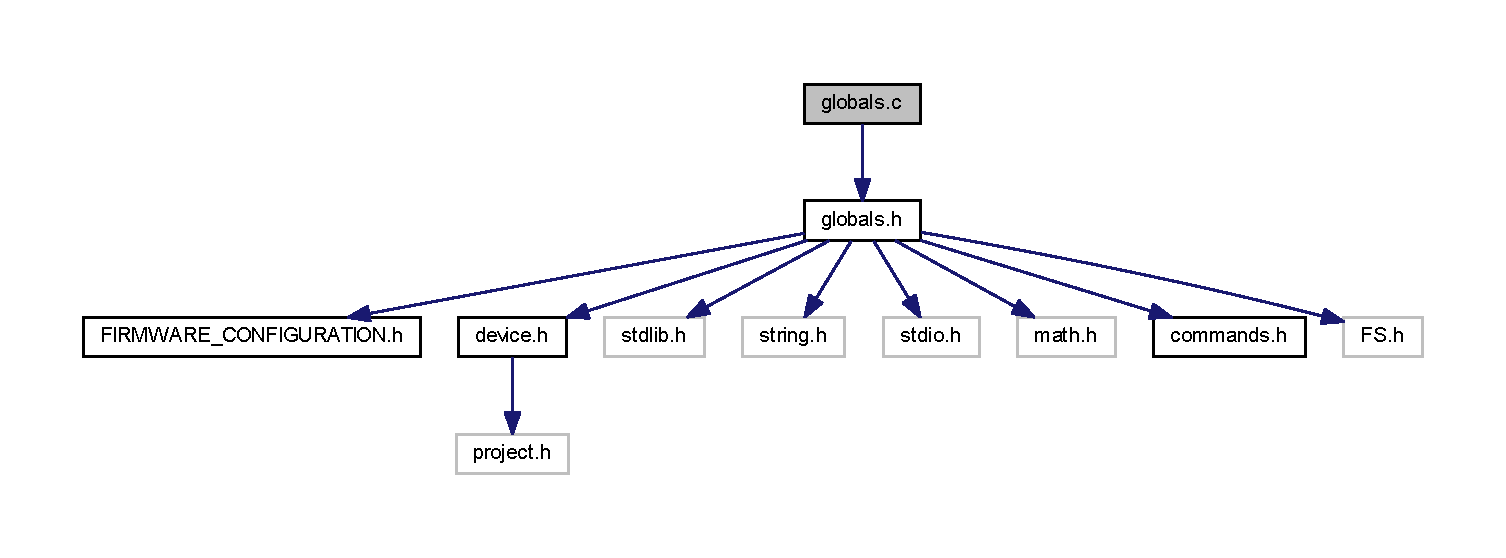
\includegraphics[width=350pt]{globals_8c__incl}
\end{center}
\end{figure}
\subsection*{Variables}
\begin{DoxyCompactItemize}
\item 
\mbox{\label{globals_8c_a975e5cde4f157d8bbdbde3c03227f3de}} 
struct \textbf{ st\+\_\+ref} {\bfseries g\+\_\+ref} [\textbf{ N\+U\+M\+\_\+\+O\+F\+\_\+\+M\+O\+T\+O\+RS}]
\item 
\mbox{\label{globals_8c_ab40c607c340b011a96046994f4b2229c}} 
struct \textbf{ st\+\_\+ref} {\bfseries g\+\_\+ref\+New} [\textbf{ N\+U\+M\+\_\+\+O\+F\+\_\+\+M\+O\+T\+O\+RS}]
\item 
struct \textbf{ st\+\_\+ref} \textbf{ g\+\_\+ref\+Old} [\textbf{ N\+U\+M\+\_\+\+O\+F\+\_\+\+M\+O\+T\+O\+RS}]
\item 
\mbox{\label{globals_8c_a6f0c00c1300c30d398231d1e76f3f780}} 
struct \textbf{ st\+\_\+meas} {\bfseries g\+\_\+meas} [\textbf{ N\+\_\+\+E\+N\+C\+O\+D\+E\+R\+\_\+\+L\+I\+N\+E\+\_\+\+M\+AX}]
\item 
struct \textbf{ st\+\_\+meas} \textbf{ g\+\_\+meas\+Old} [\textbf{ N\+\_\+\+E\+N\+C\+O\+D\+E\+R\+\_\+\+L\+I\+N\+E\+\_\+\+M\+AX}]
\item 
struct \textbf{ st\+\_\+emg\+\_\+meas} g\+\_\+emg\+\_\+meas \textbf{ g\+\_\+emg\+\_\+meas\+Old}
\item 
struct \textbf{ st\+\_\+data} \textbf{ g\+\_\+rx}
\item 
struct \textbf{ st\+\_\+eeprom} g\+\_\+mem \textbf{ c\+\_\+mem}
\item 
struct \textbf{ st\+\_\+calib} \textbf{ calib}
\item 
\mbox{\label{globals_8c_a0e9a576515332f8bd83ae6a2fe0164aa}} 
struct \textbf{ st\+\_\+filter} {\bfseries filt\+\_\+v} [\textbf{ N\+U\+M\+\_\+\+O\+F\+\_\+\+M\+O\+T\+O\+RS}]
\item 
\mbox{\label{globals_8c_a503852d956ef1e03f4a9d8b91db248fc}} 
struct \textbf{ st\+\_\+filter} {\bfseries filt\+\_\+curr\+\_\+diff} [\textbf{ N\+U\+M\+\_\+\+O\+F\+\_\+\+M\+O\+T\+O\+RS}]
\item 
struct \textbf{ st\+\_\+filter} \textbf{ filt\+\_\+i} [\textbf{ N\+U\+M\+\_\+\+O\+F\+\_\+\+M\+O\+T\+O\+RS}]
\item 
struct \textbf{ st\+\_\+filter} \textbf{ filt\+\_\+vel} [\textbf{ N\+U\+M\+\_\+\+O\+F\+\_\+\+S\+E\+N\+S\+O\+RS}]
\item 
struct \textbf{ st\+\_\+filter} \textbf{ filt\+\_\+emg} [\textbf{ N\+U\+M\+\_\+\+O\+F\+\_\+\+I\+N\+P\+U\+T\+\_\+\+E\+M\+GS}+\textbf{ N\+U\+M\+\_\+\+O\+F\+\_\+\+A\+D\+D\+I\+T\+I\+O\+N\+A\+L\+\_\+\+E\+M\+GS}]
\item 
uint16 \textbf{ timer\+\_\+value}
\item 
uint16 \textbf{ timer\+\_\+value0}
\item 
float \textbf{ cycle\+\_\+time}
\item 
int32 \textbf{ dev\+\_\+tension} [\textbf{ N\+U\+M\+\_\+\+O\+F\+\_\+\+M\+O\+T\+O\+RS}]
\item 
uint8 \textbf{ dev\+\_\+pwm\+\_\+limit} [\textbf{ N\+U\+M\+\_\+\+O\+F\+\_\+\+M\+O\+T\+O\+RS}]
\item 
uint8 \textbf{ dev\+\_\+pwm\+\_\+sat} [\textbf{ N\+U\+M\+\_\+\+O\+F\+\_\+\+M\+O\+T\+O\+RS}] = \{100,100\}
\item 
int32 \textbf{ dev\+\_\+tension\+\_\+f} [\textbf{ N\+U\+M\+\_\+\+O\+F\+\_\+\+M\+O\+T\+O\+RS}]
\item 
int32 \textbf{ pow\+\_\+tension} [\textbf{ N\+U\+M\+\_\+\+O\+F\+\_\+\+M\+O\+T\+O\+RS}]
\item 
\textbf{ counter\+\_\+status} C\+Y\+D\+A\+TA \textbf{ cycles\+\_\+status} = \textbf{ N\+O\+NE}
\item 
\textbf{ emg\+\_\+status} C\+Y\+D\+A\+TA \textbf{ emg\+\_\+1\+\_\+status} = \textbf{ R\+E\+S\+ET}
\item 
\textbf{ emg\+\_\+status} C\+Y\+D\+A\+TA \textbf{ emg\+\_\+2\+\_\+status} = \textbf{ R\+E\+S\+ET}
\item 
C\+Y\+B\+IT \textbf{ reset\+\_\+last\+\_\+value\+\_\+flag}
\item 
C\+Y\+B\+IT \textbf{ tension\+\_\+valid}
\item 
C\+Y\+B\+IT \textbf{ interrupt\+\_\+flag} = F\+A\+L\+SE
\item 
C\+Y\+B\+IT \textbf{ cycles\+\_\+interrupt\+\_\+flag} = F\+A\+L\+SE
\item 
uint8 \textbf{ maintenance\+\_\+flag} = F\+A\+L\+SE
\item 
C\+Y\+B\+IT \textbf{ can\+\_\+write} = T\+R\+UE
\item 
uint8 \textbf{ rest\+\_\+enabled}
\item 
uint8 \textbf{ forced\+\_\+open}
\item 
uint8 \textbf{ battery\+\_\+low\+\_\+\+SoC} = F\+A\+L\+SE
\item 
uint8 \textbf{ change\+\_\+ext\+\_\+ref\+\_\+flag} = F\+A\+L\+SE
\item 
C\+Y\+B\+IT \textbf{ reset\+\_\+\+P\+So\+C\+\_\+flag} = F\+A\+L\+SE
\item 
\mbox{\label{globals_8c_a2fbad668712e226379890e1debdc9ff2}} 
int16 {\bfseries A\+D\+C\+\_\+buf} [N\+U\+M\+\_\+\+O\+F\+\_\+\+A\+D\+C\+\_\+\+C\+H\+A\+N\+N\+E\+L\+S\+\_\+\+M\+AX]
\item 
uint8 \textbf{ N\+U\+M\+\_\+\+O\+F\+\_\+\+A\+N\+A\+L\+O\+G\+\_\+\+I\+N\+P\+U\+TS} = 4
\item 
int8 \textbf{ pwm\+\_\+sign}
\item 
\mbox{\label{globals_8c_a5190337b2d433e192edc68cf3d603ede}} 
uint32 {\bfseries data\+\_\+encoder\+\_\+raw} [\textbf{ N\+\_\+\+E\+N\+C\+O\+D\+E\+R\+S\+\_\+\+P\+E\+R\+\_\+\+L\+I\+N\+E\+\_\+\+M\+AX}]
\item 
\mbox{\label{globals_8c_ae62a59fe712aba1b45a5358ece0b3d35}} 
uint8 {\bfseries N\+\_\+\+Encoder\+\_\+\+Line\+\_\+\+Connected} [\textbf{ N\+\_\+\+E\+N\+C\+O\+D\+E\+R\+\_\+\+L\+I\+N\+E\+\_\+\+M\+AX}]
\item 
\mbox{\label{globals_8c_a7bf300fb19b8dd8db6783ef124605540}} 
uint16 {\bfseries Encoder\+\_\+\+Value} [\textbf{ N\+\_\+\+E\+N\+C\+O\+D\+E\+R\+\_\+\+L\+I\+N\+E\+\_\+\+M\+AX}][\textbf{ N\+\_\+\+E\+N\+C\+O\+D\+E\+R\+S\+\_\+\+P\+E\+R\+\_\+\+L\+I\+N\+E\+\_\+\+M\+AX}]
\item 
\mbox{\label{globals_8c_a269cff8427d6a8902a38dc258d649f06}} 
uint8 {\bfseries Encoder\+\_\+\+Check} [\textbf{ N\+\_\+\+E\+N\+C\+O\+D\+E\+R\+\_\+\+L\+I\+N\+E\+\_\+\+M\+AX}][\textbf{ N\+\_\+\+E\+N\+C\+O\+D\+E\+R\+S\+\_\+\+P\+E\+R\+\_\+\+L\+I\+N\+E\+\_\+\+M\+AX}]
\item 
int32 \textbf{ rest\+\_\+pos\+\_\+curr\+\_\+ref}
\item 
\mbox{\label{globals_8c_a28568209e5c79332f574608aafcd14ec}} 
F\+S\+\_\+\+F\+I\+LE $\ast$ {\bfseries p\+File}
\item 
\mbox{\label{globals_8c_a93ea3c816e507e10c5a48cb79d624863}} 
char {\bfseries sd\+File} [100] = \char`\"{}\char`\"{}
\item 
\mbox{\label{globals_8c_ad49779e5c549cf4cb332a929eacc6b71}} 
char {\bfseries sd\+Param} [100] = \char`\"{}\char`\"{}
\item 
\mbox{\label{globals_8c_a47118db87acd24ae6dac18b036f360ec}} 
uint8 {\bfseries N\+\_\+\+I\+M\+U\+\_\+\+Connected}
\item 
\mbox{\label{globals_8c_a99668f3210aba0be3baec19486621bce}} 
uint8 {\bfseries I\+M\+U\+\_\+connected} [N\+\_\+\+I\+M\+U\+\_\+\+M\+AX]
\item 
\mbox{\label{globals_8c_a86272fcfcab512d38a11824196df4bbc}} 
int {\bfseries imus\+\_\+data\+\_\+size}
\item 
\mbox{\label{globals_8c_aca96c483c3e269e3805aa861ced0aef5}} 
int {\bfseries single\+\_\+imu\+\_\+size} [N\+\_\+\+I\+M\+U\+\_\+\+M\+AX]
\item 
\mbox{\label{globals_8c_ab72cce926a6439eda41315f45a9c379c}} 
struct \textbf{ st\+\_\+imu\+\_\+data} {\bfseries g\+\_\+imu} [N\+\_\+\+I\+M\+U\+\_\+\+M\+AX]
\item 
\mbox{\label{globals_8c_abb00fd907d732c0691940f718e231178}} 
struct \textbf{ st\+\_\+imu\+\_\+data} {\bfseries g\+\_\+imu\+New} [N\+\_\+\+I\+M\+U\+\_\+\+M\+AX]
\item 
\mbox{\label{globals_8c_a187c605f3898cf11e09f6f469c265920}} 
uint8 {\bfseries Accel} [N\+\_\+\+I\+M\+U\+\_\+\+M\+AX][6]
\item 
\mbox{\label{globals_8c_a49dba88a31d1b3b4190065b9ef1649fe}} 
uint8 {\bfseries Gyro} [N\+\_\+\+I\+M\+U\+\_\+\+M\+AX][6]
\item 
\mbox{\label{globals_8c_a5d88408ccb73729f049a52b4d1daaadf}} 
uint8 {\bfseries Mag} [N\+\_\+\+I\+M\+U\+\_\+\+M\+AX][6]
\item 
\mbox{\label{globals_8c_a1e598e1bdae5fe927fbd1f396161f3a6}} 
uint8 {\bfseries Mag\+Cal} [N\+\_\+\+I\+M\+U\+\_\+\+M\+AX][3]
\item 
\mbox{\label{globals_8c_af5f2d49e123a057d358297a34194ebdc}} 
uint8 {\bfseries Temp} [N\+\_\+\+I\+M\+U\+\_\+\+M\+AX][2]
\item 
\mbox{\label{globals_8c_a79179edea7394e7176f8768b1b0f6f92}} 
float {\bfseries Quat} [N\+\_\+\+I\+M\+U\+\_\+\+M\+AX][4]
\end{DoxyCompactItemize}


\subsection{Detailed Description}
Global variables. 

\begin{DoxyDate}{Date}
October 01, 2017 
\end{DoxyDate}
\begin{DoxyAuthor}{Author}
{\itshape Centro \char`\"{}\+E.\+Piaggio\char`\"{}} 
\end{DoxyAuthor}
\begin{DoxyCopyright}{Copyright}
(C) 2012-\/2016 qbrobotics. All rights reserved. 

(C) 2017-\/2019 Centro \char`\"{}\+E.\+Piaggio\char`\"{}. All rights reserved. 
\end{DoxyCopyright}


\subsection{Variable Documentation}
\mbox{\label{globals_8c_ab4765549a3f6990d35f3d0740263b254}} 
\index{globals.\+c@{globals.\+c}!battery\+\_\+low\+\_\+\+SoC@{battery\+\_\+low\+\_\+\+SoC}}
\index{battery\+\_\+low\+\_\+\+SoC@{battery\+\_\+low\+\_\+\+SoC}!globals.\+c@{globals.\+c}}
\subsubsection{battery\+\_\+low\+\_\+\+SoC}
{\footnotesize\ttfamily uint8 battery\+\_\+low\+\_\+\+SoC = F\+A\+L\+SE}

Battery low State of Charge flag (re-\/open terminal device when active). \mbox{\label{globals_8c_a3ad3057028e3ab399e1d1549a8d67ab9}} 
\index{globals.\+c@{globals.\+c}!c\+\_\+mem@{c\+\_\+mem}}
\index{c\+\_\+mem@{c\+\_\+mem}!globals.\+c@{globals.\+c}}
\subsubsection{c\+\_\+mem}
{\footnotesize\ttfamily struct \textbf{ st\+\_\+eeprom} g\+\_\+mem c\+\_\+mem}

Memory parameters. \mbox{\label{globals_8c_aed96fdd8308fe2c4fc07c3b5db1c7bbb}} 
\index{globals.\+c@{globals.\+c}!calib@{calib}}
\index{calib@{calib}!globals.\+c@{globals.\+c}}
\subsubsection{calib}
{\footnotesize\ttfamily struct \textbf{ st\+\_\+calib} calib}

Calibration variables. \mbox{\label{globals_8c_acd57396ca1b2a02a76877acecd29ddb0}} 
\index{globals.\+c@{globals.\+c}!can\+\_\+write@{can\+\_\+write}}
\index{can\+\_\+write@{can\+\_\+write}!globals.\+c@{globals.\+c}}
\subsubsection{can\+\_\+write}
{\footnotesize\ttfamily C\+Y\+B\+IT can\+\_\+write = T\+R\+UE}

Write to E\+E\+P\+R\+OM flag. \mbox{\label{globals_8c_a55787e40db60be586171023875f15130}} 
\index{globals.\+c@{globals.\+c}!change\+\_\+ext\+\_\+ref\+\_\+flag@{change\+\_\+ext\+\_\+ref\+\_\+flag}}
\index{change\+\_\+ext\+\_\+ref\+\_\+flag@{change\+\_\+ext\+\_\+ref\+\_\+flag}!globals.\+c@{globals.\+c}}
\subsubsection{change\+\_\+ext\+\_\+ref\+\_\+flag}
{\footnotesize\ttfamily uint8 change\+\_\+ext\+\_\+ref\+\_\+flag = F\+A\+L\+SE}

This flag is set when an external reference command is received. \mbox{\label{globals_8c_a910e6d34a0bb2e8dbaf576e06bdf56f5}} 
\index{globals.\+c@{globals.\+c}!cycle\+\_\+time@{cycle\+\_\+time}}
\index{cycle\+\_\+time@{cycle\+\_\+time}!globals.\+c@{globals.\+c}}
\subsubsection{cycle\+\_\+time}
{\footnotesize\ttfamily float cycle\+\_\+time}

Variable used to calculate how much time a cycle takes. \mbox{\label{globals_8c_a9c58c534e60c7991a92a13d012e7ef86}} 
\index{globals.\+c@{globals.\+c}!cycles\+\_\+interrupt\+\_\+flag@{cycles\+\_\+interrupt\+\_\+flag}}
\index{cycles\+\_\+interrupt\+\_\+flag@{cycles\+\_\+interrupt\+\_\+flag}!globals.\+c@{globals.\+c}}
\subsubsection{cycles\+\_\+interrupt\+\_\+flag}
{\footnotesize\ttfamily C\+Y\+B\+IT cycles\+\_\+interrupt\+\_\+flag = F\+A\+L\+SE}

Cycles timer interrupt flag enabler. \mbox{\label{globals_8c_a9087b28d15f17c6475922ba6943b14f3}} 
\index{globals.\+c@{globals.\+c}!cycles\+\_\+status@{cycles\+\_\+status}}
\index{cycles\+\_\+status@{cycles\+\_\+status}!globals.\+c@{globals.\+c}}
\subsubsection{cycles\+\_\+status}
{\footnotesize\ttfamily \textbf{ counter\+\_\+status} C\+Y\+D\+A\+TA cycles\+\_\+status = \textbf{ N\+O\+NE}}

Cycles counter state machine status. \mbox{\label{globals_8c_ac7fdc35fc8e87ead9b45028d6034fb1b}} 
\index{globals.\+c@{globals.\+c}!dev\+\_\+pwm\+\_\+limit@{dev\+\_\+pwm\+\_\+limit}}
\index{dev\+\_\+pwm\+\_\+limit@{dev\+\_\+pwm\+\_\+limit}!globals.\+c@{globals.\+c}}
\subsubsection{dev\+\_\+pwm\+\_\+limit}
{\footnotesize\ttfamily uint8 dev\+\_\+pwm\+\_\+limit[\textbf{ N\+U\+M\+\_\+\+O\+F\+\_\+\+M\+O\+T\+O\+RS}]}

Device pwm limit. It may change during execution. \mbox{\label{globals_8c_a2e254e60f92958e2fdec99dde626dca6}} 
\index{globals.\+c@{globals.\+c}!dev\+\_\+pwm\+\_\+sat@{dev\+\_\+pwm\+\_\+sat}}
\index{dev\+\_\+pwm\+\_\+sat@{dev\+\_\+pwm\+\_\+sat}!globals.\+c@{globals.\+c}}
\subsubsection{dev\+\_\+pwm\+\_\+sat}
{\footnotesize\ttfamily uint8 dev\+\_\+pwm\+\_\+sat[\textbf{ N\+U\+M\+\_\+\+O\+F\+\_\+\+M\+O\+T\+O\+RS}] = \{100,100\}}

Device pwm saturation. By default the saturation value must not exceed 100. \mbox{\label{globals_8c_aada869b6650bdd87ca481109ae08231c}} 
\index{globals.\+c@{globals.\+c}!dev\+\_\+tension@{dev\+\_\+tension}}
\index{dev\+\_\+tension@{dev\+\_\+tension}!globals.\+c@{globals.\+c}}
\subsubsection{dev\+\_\+tension}
{\footnotesize\ttfamily int32 dev\+\_\+tension[\textbf{ N\+U\+M\+\_\+\+O\+F\+\_\+\+M\+O\+T\+O\+RS}]}

Power supply tension. \mbox{\label{globals_8c_aa2494c7cd8f096ca7f2ead0a1430a597}} 
\index{globals.\+c@{globals.\+c}!dev\+\_\+tension\+\_\+f@{dev\+\_\+tension\+\_\+f}}
\index{dev\+\_\+tension\+\_\+f@{dev\+\_\+tension\+\_\+f}!globals.\+c@{globals.\+c}}
\subsubsection{dev\+\_\+tension\+\_\+f}
{\footnotesize\ttfamily int32 dev\+\_\+tension\+\_\+f[\textbf{ N\+U\+M\+\_\+\+O\+F\+\_\+\+M\+O\+T\+O\+RS}]}

Filtered power supply tension. \mbox{\label{globals_8c_a433230c4343adf14967e6f4f9082b199}} 
\index{globals.\+c@{globals.\+c}!emg\+\_\+1\+\_\+status@{emg\+\_\+1\+\_\+status}}
\index{emg\+\_\+1\+\_\+status@{emg\+\_\+1\+\_\+status}!globals.\+c@{globals.\+c}}
\subsubsection{emg\+\_\+1\+\_\+status}
{\footnotesize\ttfamily \textbf{ emg\+\_\+status} C\+Y\+D\+A\+TA emg\+\_\+1\+\_\+status = \textbf{ R\+E\+S\+ET}}

First E\+MG sensor status. \mbox{\label{globals_8c_a7eef8180f636a73854d52b58e2be4e51}} 
\index{globals.\+c@{globals.\+c}!emg\+\_\+2\+\_\+status@{emg\+\_\+2\+\_\+status}}
\index{emg\+\_\+2\+\_\+status@{emg\+\_\+2\+\_\+status}!globals.\+c@{globals.\+c}}
\subsubsection{emg\+\_\+2\+\_\+status}
{\footnotesize\ttfamily \textbf{ emg\+\_\+status} C\+Y\+D\+A\+TA emg\+\_\+2\+\_\+status = \textbf{ R\+E\+S\+ET}}

Second E\+MG sensor status. \mbox{\label{globals_8c_aad3d2663356b48553e2b22e0a9fd917e}} 
\index{globals.\+c@{globals.\+c}!filt\+\_\+emg@{filt\+\_\+emg}}
\index{filt\+\_\+emg@{filt\+\_\+emg}!globals.\+c@{globals.\+c}}
\subsubsection{filt\+\_\+emg}
{\footnotesize\ttfamily struct \textbf{ st\+\_\+filter} filt\+\_\+emg[\textbf{ N\+U\+M\+\_\+\+O\+F\+\_\+\+I\+N\+P\+U\+T\+\_\+\+E\+M\+GS}+\textbf{ N\+U\+M\+\_\+\+O\+F\+\_\+\+A\+D\+D\+I\+T\+I\+O\+N\+A\+L\+\_\+\+E\+M\+GS}]}

E\+MG filter variables. \mbox{\label{globals_8c_ad09553d6780c43066a9ac4385658bcf1}} 
\index{globals.\+c@{globals.\+c}!filt\+\_\+i@{filt\+\_\+i}}
\index{filt\+\_\+i@{filt\+\_\+i}!globals.\+c@{globals.\+c}}
\subsubsection{filt\+\_\+i}
{\footnotesize\ttfamily struct \textbf{ st\+\_\+filter} filt\+\_\+i[\textbf{ N\+U\+M\+\_\+\+O\+F\+\_\+\+M\+O\+T\+O\+RS}]}

Voltage and current filter variables. \mbox{\label{globals_8c_af2dc9b0614aeaf7a377d209416bee61c}} 
\index{globals.\+c@{globals.\+c}!filt\+\_\+vel@{filt\+\_\+vel}}
\index{filt\+\_\+vel@{filt\+\_\+vel}!globals.\+c@{globals.\+c}}
\subsubsection{filt\+\_\+vel}
{\footnotesize\ttfamily struct \textbf{ st\+\_\+filter} filt\+\_\+vel[\textbf{ N\+U\+M\+\_\+\+O\+F\+\_\+\+S\+E\+N\+S\+O\+RS}]}

Velocity filter variables. \mbox{\label{globals_8c_a0f13b80a0c329fa3176eb1e72ef36fb8}} 
\index{globals.\+c@{globals.\+c}!forced\+\_\+open@{forced\+\_\+open}}
\index{forced\+\_\+open@{forced\+\_\+open}!globals.\+c@{globals.\+c}}
\subsubsection{forced\+\_\+open}
{\footnotesize\ttfamily uint8 forced\+\_\+open}

Forced open flag (used in position with rest position control). \mbox{\label{globals_8c_a85e15a194417ebcd15f662bd9bcfdded}} 
\index{globals.\+c@{globals.\+c}!g\+\_\+emg\+\_\+meas\+Old@{g\+\_\+emg\+\_\+meas\+Old}}
\index{g\+\_\+emg\+\_\+meas\+Old@{g\+\_\+emg\+\_\+meas\+Old}!globals.\+c@{globals.\+c}}
\subsubsection{g\+\_\+emg\+\_\+meas\+Old}
{\footnotesize\ttfamily struct \textbf{ st\+\_\+emg\+\_\+meas} g\+\_\+emg\+\_\+meas g\+\_\+emg\+\_\+meas\+Old}

E\+MG Measurements. \mbox{\label{globals_8c_a7b175385b2b9418fa7159c72d0f470fd}} 
\index{globals.\+c@{globals.\+c}!g\+\_\+meas\+Old@{g\+\_\+meas\+Old}}
\index{g\+\_\+meas\+Old@{g\+\_\+meas\+Old}!globals.\+c@{globals.\+c}}
\subsubsection{g\+\_\+meas\+Old}
{\footnotesize\ttfamily struct \textbf{ st\+\_\+meas} g\+\_\+meas\+Old[\textbf{ N\+\_\+\+E\+N\+C\+O\+D\+E\+R\+\_\+\+L\+I\+N\+E\+\_\+\+M\+AX}]}

Measurements. \mbox{\label{globals_8c_aab927f8d9bc1a835daed821aa97b9335}} 
\index{globals.\+c@{globals.\+c}!g\+\_\+ref\+Old@{g\+\_\+ref\+Old}}
\index{g\+\_\+ref\+Old@{g\+\_\+ref\+Old}!globals.\+c@{globals.\+c}}
\subsubsection{g\+\_\+ref\+Old}
{\footnotesize\ttfamily struct \textbf{ st\+\_\+ref} g\+\_\+ref\+Old[\textbf{ N\+U\+M\+\_\+\+O\+F\+\_\+\+M\+O\+T\+O\+RS}]}

Reference variables. \mbox{\label{globals_8c_aa963ce8fafc11e104eb7ee22982d0345}} 
\index{globals.\+c@{globals.\+c}!g\+\_\+rx@{g\+\_\+rx}}
\index{g\+\_\+rx@{g\+\_\+rx}!globals.\+c@{globals.\+c}}
\subsubsection{g\+\_\+rx}
{\footnotesize\ttfamily struct \textbf{ st\+\_\+data} g\+\_\+rx}

Incoming/\+Outcoming data. \mbox{\label{globals_8c_a1e6fda88dfdabc63859f8907eb702920}} 
\index{globals.\+c@{globals.\+c}!interrupt\+\_\+flag@{interrupt\+\_\+flag}}
\index{interrupt\+\_\+flag@{interrupt\+\_\+flag}!globals.\+c@{globals.\+c}}
\subsubsection{interrupt\+\_\+flag}
{\footnotesize\ttfamily C\+Y\+B\+IT interrupt\+\_\+flag = F\+A\+L\+SE}

Interrupt flag enabler. \mbox{\label{globals_8c_a7bdd0aaa2a8c38bd61f34d76d3a69dbf}} 
\index{globals.\+c@{globals.\+c}!maintenance\+\_\+flag@{maintenance\+\_\+flag}}
\index{maintenance\+\_\+flag@{maintenance\+\_\+flag}!globals.\+c@{globals.\+c}}
\subsubsection{maintenance\+\_\+flag}
{\footnotesize\ttfamily uint8 maintenance\+\_\+flag = F\+A\+L\+SE}

Maintenance flag. \mbox{\label{globals_8c_ab302ef69391ec5a0b59dadb9c7d2a3ef}} 
\index{globals.\+c@{globals.\+c}!N\+U\+M\+\_\+\+O\+F\+\_\+\+A\+N\+A\+L\+O\+G\+\_\+\+I\+N\+P\+U\+TS@{N\+U\+M\+\_\+\+O\+F\+\_\+\+A\+N\+A\+L\+O\+G\+\_\+\+I\+N\+P\+U\+TS}}
\index{N\+U\+M\+\_\+\+O\+F\+\_\+\+A\+N\+A\+L\+O\+G\+\_\+\+I\+N\+P\+U\+TS@{N\+U\+M\+\_\+\+O\+F\+\_\+\+A\+N\+A\+L\+O\+G\+\_\+\+I\+N\+P\+U\+TS}!globals.\+c@{globals.\+c}}
\subsubsection{N\+U\+M\+\_\+\+O\+F\+\_\+\+A\+N\+A\+L\+O\+G\+\_\+\+I\+N\+P\+U\+TS}
{\footnotesize\ttfamily uint8 N\+U\+M\+\_\+\+O\+F\+\_\+\+A\+N\+A\+L\+O\+G\+\_\+\+I\+N\+P\+U\+TS = 4}

A\+DC measurements buffer. \mbox{\label{globals_8c_a1c717f431f1d1ea4a500f6027102d001}} 
\index{globals.\+c@{globals.\+c}!pow\+\_\+tension@{pow\+\_\+tension}}
\index{pow\+\_\+tension@{pow\+\_\+tension}!globals.\+c@{globals.\+c}}
\subsubsection{pow\+\_\+tension}
{\footnotesize\ttfamily int32 pow\+\_\+tension[\textbf{ N\+U\+M\+\_\+\+O\+F\+\_\+\+M\+O\+T\+O\+RS}]}

Computed power supply tension. \mbox{\label{globals_8c_a8ac7ad7c894db750e93bc745818e26ca}} 
\index{globals.\+c@{globals.\+c}!pwm\+\_\+sign@{pwm\+\_\+sign}}
\index{pwm\+\_\+sign@{pwm\+\_\+sign}!globals.\+c@{globals.\+c}}
\subsubsection{pwm\+\_\+sign}
{\footnotesize\ttfamily int8 pwm\+\_\+sign}

A\+DC currently configured channels. Sign of pwm driven. Used to obtain current sign. \mbox{\label{globals_8c_aa89a782cfe75ce7970236babd308fe69}} 
\index{globals.\+c@{globals.\+c}!reset\+\_\+last\+\_\+value\+\_\+flag@{reset\+\_\+last\+\_\+value\+\_\+flag}}
\index{reset\+\_\+last\+\_\+value\+\_\+flag@{reset\+\_\+last\+\_\+value\+\_\+flag}!globals.\+c@{globals.\+c}}
\subsubsection{reset\+\_\+last\+\_\+value\+\_\+flag}
{\footnotesize\ttfamily C\+Y\+B\+IT reset\+\_\+last\+\_\+value\+\_\+flag}

This flag is set when the encoders last values must be resetted. \mbox{\label{globals_8c_a7f81d1d66186b1c7cd358ea7cfff2caf}} 
\index{globals.\+c@{globals.\+c}!reset\+\_\+\+P\+So\+C\+\_\+flag@{reset\+\_\+\+P\+So\+C\+\_\+flag}}
\index{reset\+\_\+\+P\+So\+C\+\_\+flag@{reset\+\_\+\+P\+So\+C\+\_\+flag}!globals.\+c@{globals.\+c}}
\subsubsection{reset\+\_\+\+P\+So\+C\+\_\+flag}
{\footnotesize\ttfamily C\+Y\+B\+IT reset\+\_\+\+P\+So\+C\+\_\+flag = F\+A\+L\+SE}

This flag is set when a board fw reset is necessary. \mbox{\label{globals_8c_a1f8839fadee52a47a0042eaa695c3f3a}} 
\index{globals.\+c@{globals.\+c}!rest\+\_\+enabled@{rest\+\_\+enabled}}
\index{rest\+\_\+enabled@{rest\+\_\+enabled}!globals.\+c@{globals.\+c}}
\subsubsection{rest\+\_\+enabled}
{\footnotesize\ttfamily uint8 rest\+\_\+enabled}

Rest position flag. \mbox{\label{globals_8c_a485e5b90bbfb79aa97f874873cd6c93a}} 
\index{globals.\+c@{globals.\+c}!rest\+\_\+pos\+\_\+curr\+\_\+ref@{rest\+\_\+pos\+\_\+curr\+\_\+ref}}
\index{rest\+\_\+pos\+\_\+curr\+\_\+ref@{rest\+\_\+pos\+\_\+curr\+\_\+ref}!globals.\+c@{globals.\+c}}
\subsubsection{rest\+\_\+pos\+\_\+curr\+\_\+ref}
{\footnotesize\ttfamily int32 rest\+\_\+pos\+\_\+curr\+\_\+ref}

Rest position current reference. \mbox{\label{globals_8c_ac42fa606610c2600210d9b7b2c1d0882}} 
\index{globals.\+c@{globals.\+c}!tension\+\_\+valid@{tension\+\_\+valid}}
\index{tension\+\_\+valid@{tension\+\_\+valid}!globals.\+c@{globals.\+c}}
\subsubsection{tension\+\_\+valid}
{\footnotesize\ttfamily C\+Y\+B\+IT tension\+\_\+valid}

Tension validation bit. \mbox{\label{globals_8c_a2c95347784600e4a45d481b37eeeef4b}} 
\index{globals.\+c@{globals.\+c}!timer\+\_\+value@{timer\+\_\+value}}
\index{timer\+\_\+value@{timer\+\_\+value}!globals.\+c@{globals.\+c}}
\subsubsection{timer\+\_\+value}
{\footnotesize\ttfamily uint16 timer\+\_\+value}

End time of the firmware main loop. \mbox{\label{globals_8c_a82c5883d1d4a600a1073686f917a812d}} 
\index{globals.\+c@{globals.\+c}!timer\+\_\+value0@{timer\+\_\+value0}}
\index{timer\+\_\+value0@{timer\+\_\+value0}!globals.\+c@{globals.\+c}}
\subsubsection{timer\+\_\+value0}
{\footnotesize\ttfamily uint16 timer\+\_\+value0}

Start time of the firmware main loop. 
\section{globals.\+h File Reference}
\label{globals_8h}\index{globals.\+h@{globals.\+h}}


Global definitions and macros are set in this file.  


{\ttfamily \#include \char`\"{}F\+I\+R\+M\+W\+A\+R\+E\+\_\+\+C\+O\+N\+F\+I\+G\+U\+R\+A\+T\+I\+O\+N.\+h\char`\"{}}\newline
{\ttfamily \#include \char`\"{}device.\+h\char`\"{}}\newline
{\ttfamily \#include \char`\"{}stdlib.\+h\char`\"{}}\newline
{\ttfamily \#include \char`\"{}string.\+h\char`\"{}}\newline
{\ttfamily \#include \char`\"{}stdio.\+h\char`\"{}}\newline
{\ttfamily \#include \char`\"{}math.\+h\char`\"{}}\newline
{\ttfamily \#include \char`\"{}commands.\+h\char`\"{}}\newline
{\ttfamily \#include \char`\"{}F\+S.\+h\char`\"{}}\newline
Include dependency graph for globals.\+h\+:\nopagebreak
\begin{figure}[H]
\begin{center}
\leavevmode
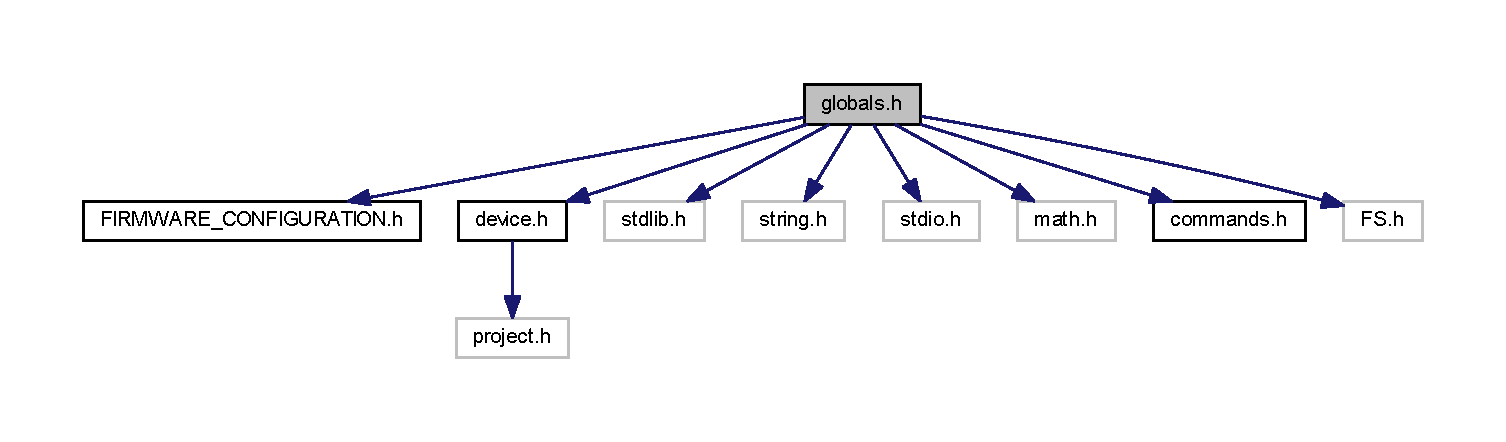
\includegraphics[width=350pt]{globals_8h__incl}
\end{center}
\end{figure}
This graph shows which files directly or indirectly include this file\+:\nopagebreak
\begin{figure}[H]
\begin{center}
\leavevmode
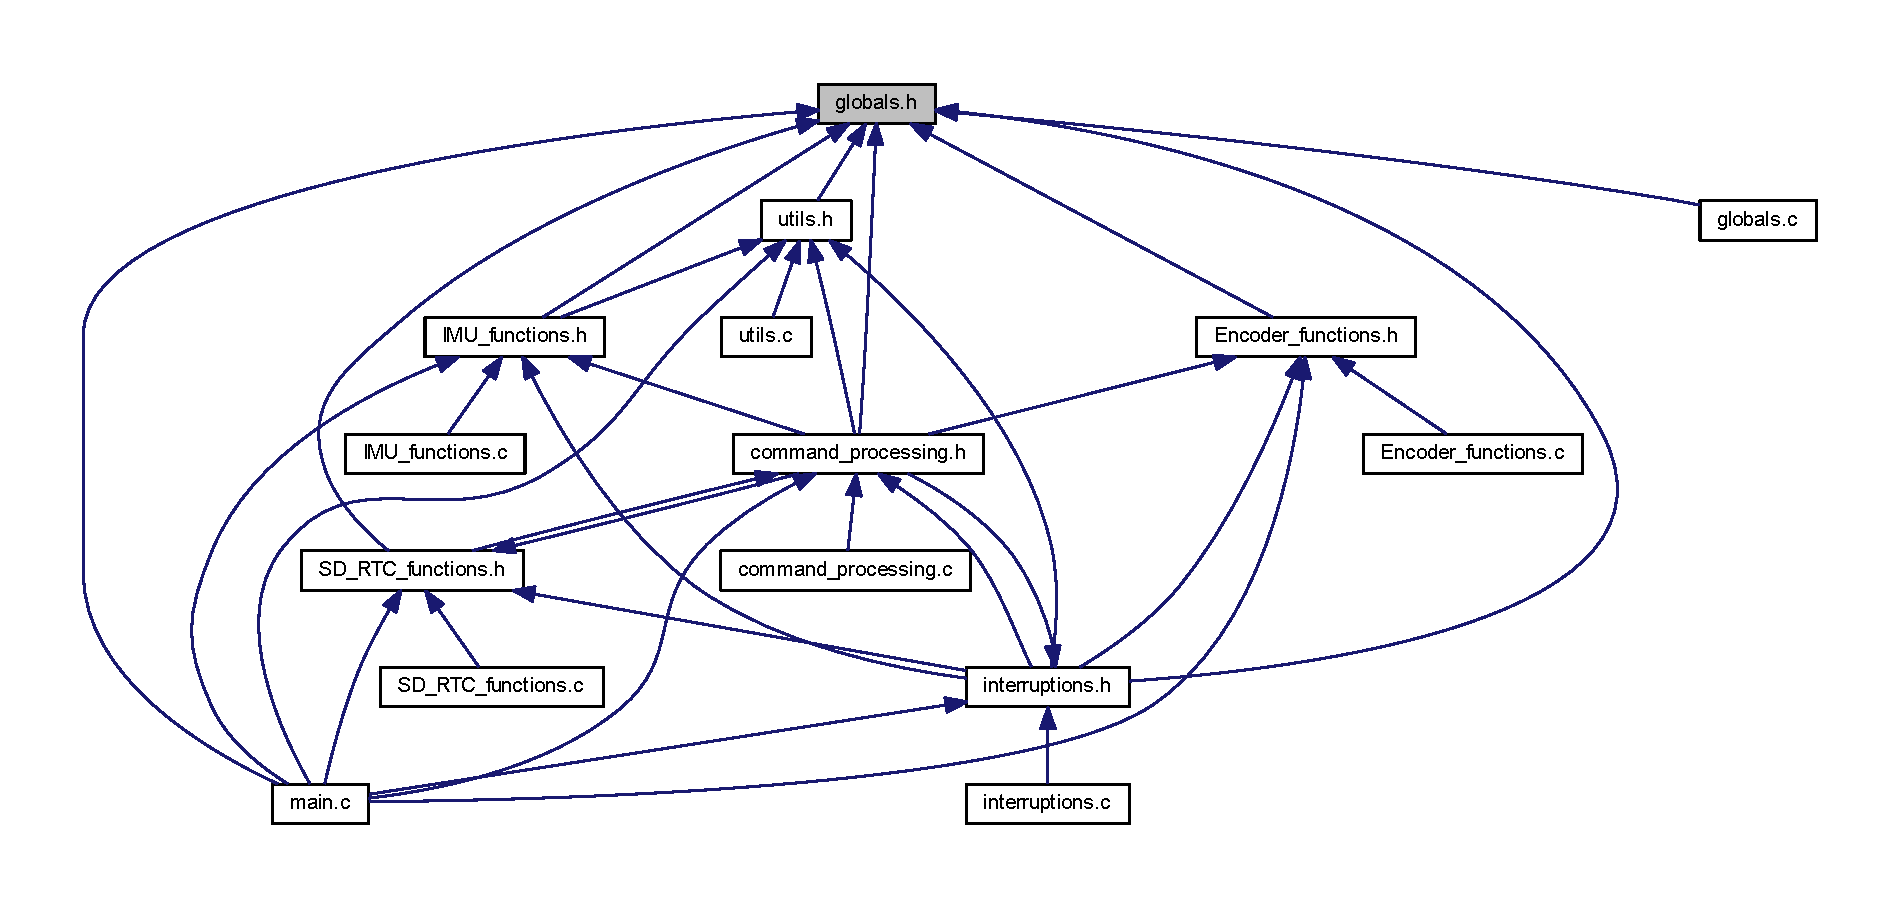
\includegraphics[width=350pt]{globals_8h__dep__incl}
\end{center}
\end{figure}
\subsection*{Data Structures}
\begin{DoxyCompactItemize}
\item 
struct \textbf{ st\+\_\+ref}
\begin{DoxyCompactList}\small\item\em Motor Reference structure. \end{DoxyCompactList}\item 
struct \textbf{ st\+\_\+meas}
\begin{DoxyCompactList}\small\item\em Measurements structure. \end{DoxyCompactList}\item 
struct \textbf{ st\+\_\+emg\+\_\+meas}
\item 
struct \textbf{ st\+\_\+data}
\begin{DoxyCompactList}\small\item\em Data sent/received structure. \end{DoxyCompactList}\item 
struct \textbf{ st\+\_\+counters}
\begin{DoxyCompactList}\small\item\em E\+E\+P\+R\+OM stored structures. \end{DoxyCompactList}\item 
struct \textbf{ st\+\_\+device}
\item 
struct \textbf{ st\+\_\+motor}
\item 
struct \textbf{ st\+\_\+encoder}
\item 
struct \textbf{ st\+\_\+emg}
\item 
struct \textbf{ st\+\_\+imu}
\item 
struct \textbf{ st\+\_\+expansion}
\item 
struct \textbf{ st\+\_\+user}
\item 
struct \textbf{ st\+\_\+\+S\+H\+\_\+spec}
\item 
struct \textbf{ st\+\_\+eeprom}
\item 
struct \textbf{ st\+\_\+imu\+\_\+data}
\item 
struct \textbf{ st\+\_\+filter}
\begin{DoxyCompactList}\small\item\em Filter structure. \end{DoxyCompactList}\item 
struct \textbf{ st\+\_\+calib}
\begin{DoxyCompactList}\small\item\em Hand calibration structure. \end{DoxyCompactList}\end{DoxyCompactItemize}
\subsection*{Macros}
\begin{DoxyCompactItemize}
\item 
\#define \textbf{ N\+U\+M\+\_\+\+O\+F\+\_\+\+M\+O\+T\+O\+RS}~2
\item 
\#define \textbf{ N\+U\+M\+\_\+\+O\+F\+\_\+\+S\+E\+N\+S\+O\+RS}~3
\item 
\#define \textbf{ N\+U\+M\+\_\+\+O\+F\+\_\+\+I\+N\+P\+U\+T\+\_\+\+E\+M\+GS}~2
\item 
\#define \textbf{ N\+U\+M\+\_\+\+O\+F\+\_\+\+A\+D\+D\+I\+T\+I\+O\+N\+A\+L\+\_\+\+E\+M\+GS}~6
\item 
\mbox{\label{globals_8h_a94a49570e3bc73b67084f1a9ae90d89a}} 
\#define {\bfseries N\+U\+M\+\_\+\+O\+F\+\_\+\+A\+D\+C\+\_\+\+C\+H\+A\+N\+N\+E\+L\+S\+\_\+\+M\+AX}~(4+\textbf{ N\+U\+M\+\_\+\+O\+F\+\_\+\+I\+N\+P\+U\+T\+\_\+\+E\+M\+GS}+\textbf{ N\+U\+M\+\_\+\+O\+F\+\_\+\+A\+D\+D\+I\+T\+I\+O\+N\+A\+L\+\_\+\+E\+M\+GS})
\item 
\#define \textbf{ N\+U\+M\+\_\+\+O\+F\+\_\+\+P\+A\+R\+A\+MS}~71
\item 
\#define \textbf{ N\+U\+M\+\_\+\+O\+F\+\_\+\+P\+A\+R\+A\+M\+S\+\_\+\+M\+E\+NU}~10
\item 
\mbox{\label{globals_8h_a8e4d7a571850d3268c9b780b171474e6}} 
\#define {\bfseries N\+\_\+\+I\+M\+U\+\_\+\+M\+AX}~5
\item 
\mbox{\label{globals_8h_a7016adad486a9166338f1667813d8b5c}} 
\#define {\bfseries N\+U\+M\+\_\+\+O\+F\+\_\+\+I\+M\+U\+\_\+\+D\+A\+TA}~5
\item 
\#define \textbf{ N\+\_\+\+E\+N\+C\+O\+D\+E\+R\+\_\+\+L\+I\+N\+E\+\_\+\+M\+AX}~2
\item 
\#define \textbf{ N\+\_\+\+E\+N\+C\+O\+D\+E\+R\+S\+\_\+\+P\+E\+R\+\_\+\+L\+I\+N\+E\+\_\+\+M\+AX}~5
\item 
\mbox{\label{globals_8h_a3b87e4129f51a9ee36bdfb06ea0a9268}} 
\#define {\bfseries N\+\_\+\+E\+N\+C\+O\+D\+E\+RS}~\textbf{ N\+U\+M\+\_\+\+O\+F\+\_\+\+S\+E\+N\+S\+O\+RS}
\item 
\#define \textbf{ C\+A\+L\+I\+B\+R\+A\+T\+I\+O\+N\+\_\+\+D\+IV}~10
\item 
\#define \textbf{ D\+I\+V\+\_\+\+I\+N\+I\+T\+\_\+\+V\+A\+L\+UE}~1
\item 
\mbox{\label{globals_8h_abf6c9afec04b86961e177e0646401ace}} 
\#define {\bfseries D\+M\+A\+\_\+\+B\+Y\+T\+E\+S\+\_\+\+P\+E\+R\+\_\+\+B\+U\+R\+ST}~2
\item 
\mbox{\label{globals_8h_ab4613f8bee68bc68fa6fe94a3ae6d568}} 
\#define {\bfseries D\+M\+A\+\_\+\+R\+E\+Q\+U\+E\+S\+T\+\_\+\+P\+E\+R\+\_\+\+B\+U\+R\+ST}~1
\item 
\mbox{\label{globals_8h_a3cc2eedb40809a1f15ad841c8abbcebf}} 
\#define {\bfseries D\+M\+A\+\_\+\+S\+R\+C\+\_\+\+B\+A\+SE}~(C\+Y\+D\+E\+V\+\_\+\+P\+E\+R\+I\+P\+H\+\_\+\+B\+A\+SE)
\item 
\mbox{\label{globals_8h_aa54e301f446a66cbf8c943d920c8e967}} 
\#define {\bfseries D\+M\+A\+\_\+\+D\+S\+T\+\_\+\+B\+A\+SE}~(C\+Y\+D\+E\+V\+\_\+\+S\+R\+A\+M\+\_\+\+B\+A\+SE)
\item 
\#define \textbf{ W\+A\+I\+T\+\_\+\+S\+T\+A\+RT}~0
\item 
\#define \textbf{ W\+A\+I\+T\+\_\+\+ID}~1
\item 
\#define \textbf{ W\+A\+I\+T\+\_\+\+L\+E\+N\+G\+TH}~2
\item 
\#define \textbf{ R\+E\+C\+E\+I\+VE}~3
\item 
\#define \textbf{ U\+N\+L\+O\+AD}~4
\item 
\#define \textbf{ S\+T\+A\+T\+E\+\_\+\+I\+N\+A\+C\+T\+I\+VE}~0
\item 
\#define \textbf{ S\+T\+A\+T\+E\+\_\+\+A\+C\+T\+I\+VE}~1
\item 
\#define \textbf{ C\+O\+U\+N\+T\+E\+R\+\_\+\+I\+NC}~2
\item 
\mbox{\label{globals_8h_a42c6406a75a89d50c9f1b9c86388565c}} 
\#define {\bfseries S\+P\+I\+\_\+\+D\+E\+L\+A\+Y\+\_\+\+L\+OW}~10
\item 
\mbox{\label{globals_8h_a054002df34537a2a4ff6f520b65f1ba4}} 
\#define {\bfseries S\+P\+I\+\_\+\+D\+E\+L\+A\+Y\+\_\+\+H\+I\+GH}~100
\item 
\mbox{\label{globals_8h_a963cfc2155941aff08c02b451042c295}} 
\#define {\bfseries E\+X\+P\+\_\+\+N\+O\+NE}~0
\item 
\mbox{\label{globals_8h_a6a936c7ef5908ffabf8be42833a3daee}} 
\#define {\bfseries E\+X\+P\+\_\+\+S\+D\+\_\+\+R\+TC}~1
\item 
\mbox{\label{globals_8h_a25767403f2ad21cf275206135269647e}} 
\#define {\bfseries E\+X\+P\+\_\+\+W\+I\+FI}~2
\item 
\mbox{\label{globals_8h_a265e7aabffe2182cd632b15dd02a9efb}} 
\#define {\bfseries E\+X\+P\+\_\+\+O\+T\+H\+ER}~3
\item 
\mbox{\label{globals_8h_a20e659d92cc540a195717f8cc2dd4b42}} 
\#define {\bfseries D\+R\+I\+V\+E\+R\+\_\+\+M\+C33887}~0
\item 
\mbox{\label{globals_8h_a2e6a13011f6123a8f0c064e37b116880}} 
\#define {\bfseries D\+R\+I\+V\+E\+R\+\_\+\+V\+N\+H5019}~1
\item 
\mbox{\label{globals_8h_a5d1d275cfec76197e014fe4d58f2e569}} 
\#define {\bfseries R\+I\+G\+H\+T\+\_\+\+H\+A\+ND}~0
\item 
\mbox{\label{globals_8h_a2eff09387fb5d20d8af4fa186ae37c4d}} 
\#define {\bfseries L\+E\+F\+T\+\_\+\+H\+A\+ND}~1
\item 
\mbox{\label{globals_8h_aa518fecbba4980ebda2090f02ceb5e52}} 
\#define {\bfseries N\+U\+M\+\_\+\+O\+F\+\_\+\+U\+S\+E\+RS}~3
\item 
\mbox{\label{globals_8h_ac524d0f906498efbd1182856cd8c80de}} 
\#define {\bfseries G\+E\+N\+E\+R\+I\+C\+\_\+\+U\+S\+ER}~0
\item 
\mbox{\label{globals_8h_a8595fed7fe248547047c468802057a0d}} 
\#define {\bfseries M\+A\+R\+IA}~1
\item 
\mbox{\label{globals_8h_a7617063d52fc2d1ba6d0276770aec732}} 
\#define {\bfseries R\+O\+ZA}~2
\item 
\mbox{\label{globals_8h_a47a1fa8e1e5435f664749ab44e163bae}} 
\#define {\bfseries S\+O\+F\+T\+H\+A\+N\+D\+\_\+\+P\+RO}~0
\item 
\mbox{\label{globals_8h_a577f879b1a05acd55b1d56412a17e13f}} 
\#define {\bfseries G\+E\+N\+E\+R\+I\+C\+\_\+2\+\_\+\+M\+O\+T\+O\+RS}~1
\item 
\mbox{\label{globals_8h_ac5a0bd9be15f1dcd0ba86f27d3dbda50}} 
\#define {\bfseries C\+U\+FF}~2
\item 
\#define \textbf{ S\+H\+\_\+\+N1}~35
\item 
\#define \textbf{ S\+H\+\_\+\+N2}~3
\item 
\#define \textbf{ S\+H\+\_\+\+I1}~-\/1
\item 
\mbox{\label{globals_8h_a5f8f4a24628c7191c9adde97ae751bf2}} 
\#define {\bfseries S\+T\+\_\+\+D\+E\+V\+I\+CE}~0
\item 
\mbox{\label{globals_8h_a911881bfa4a82a79f351f7a8a8ea40d1}} 
\#define {\bfseries S\+T\+\_\+\+M\+O\+T\+OR}~10
\item 
\mbox{\label{globals_8h_a642639720f787f90dab85f94d4be660c}} 
\#define {\bfseries S\+T\+\_\+\+E\+N\+C\+O\+D\+ER}~20
\item 
\mbox{\label{globals_8h_afca454140c3233621eaa719a25a1c4b5}} 
\#define {\bfseries S\+T\+\_\+\+E\+MG}~30
\item 
\mbox{\label{globals_8h_a6f71b4081fa44d0458fa27e891527315}} 
\#define {\bfseries S\+T\+\_\+\+I\+MU}~40
\item 
\mbox{\label{globals_8h_a3aacefdd9f8dddbb7b55bcd39bf22792}} 
\#define {\bfseries S\+T\+\_\+\+E\+X\+P\+A\+N\+S\+I\+ON}~50
\item 
\mbox{\label{globals_8h_a16d74d98ce4fcdfb20501e89e37ff053}} 
\#define {\bfseries S\+T\+\_\+\+U\+S\+ER}~60
\item 
\mbox{\label{globals_8h_a788bae111bb48b9aa005ecf765ce1e94}} 
\#define {\bfseries S\+T\+\_\+\+S\+H\+\_\+\+S\+P\+EC}~70
\item 
\mbox{\label{globals_8h_aa93f0eb578d23995850d61f7d61c55c1}} 
\#define {\bfseries F\+A\+L\+SE}~0
\item 
\mbox{\label{globals_8h_aa8cecfc5c5c054d2875c03e77b7be15d}} 
\#define {\bfseries T\+R\+UE}~1
\item 
\#define \textbf{ D\+E\+F\+A\+U\+L\+T\+\_\+\+E\+E\+P\+R\+O\+M\+\_\+\+D\+I\+S\+P\+L\+A\+C\+E\+M\+E\+NT}~50
\item 
\#define \textbf{ E\+E\+P\+R\+O\+M\+\_\+\+B\+Y\+T\+E\+S\+\_\+\+R\+OW}~16
\item 
\#define \textbf{ E\+E\+P\+R\+O\+M\+\_\+\+C\+O\+U\+N\+T\+E\+R\+S\+\_\+\+R\+O\+WS}~5
\item 
\#define \textbf{ P\+W\+M\+\_\+\+M\+A\+X\+\_\+\+V\+A\+L\+UE}~100
\item 
\#define \textbf{ A\+N\+T\+I\+\_\+\+W\+I\+N\+D\+UP}~1000
\item 
\#define \textbf{ D\+E\+F\+A\+U\+L\+T\+\_\+\+C\+U\+R\+R\+E\+N\+T\+\_\+\+L\+I\+M\+IT}~1500
\item 
\#define \textbf{ C\+U\+R\+R\+E\+N\+T\+\_\+\+H\+Y\+S\+T\+E\+R\+E\+S\+IS}~10
\item 
\#define \textbf{ E\+M\+G\+\_\+\+S\+A\+M\+P\+L\+E\+\_\+\+T\+O\+\_\+\+D\+I\+S\+C\+A\+RD}~500
\item 
\#define \textbf{ S\+A\+M\+P\+L\+E\+S\+\_\+\+F\+O\+R\+\_\+\+M\+E\+AN}~100
\item 
\#define \textbf{ S\+A\+M\+P\+L\+E\+S\+\_\+\+F\+O\+R\+\_\+\+E\+M\+G\+\_\+\+M\+E\+AN}~1000
\item 
\#define \textbf{ R\+E\+S\+T\+\_\+\+P\+O\+S\+\_\+\+E\+R\+R\+\_\+\+T\+H\+R\+\_\+\+G\+A\+IN}~10
\item 
\#define \textbf{ P\+O\+S\+\_\+\+I\+N\+T\+E\+G\+R\+A\+L\+\_\+\+S\+A\+T\+\_\+\+L\+I\+M\+IT}~50000000
\item 
\#define \textbf{ C\+U\+R\+R\+\_\+\+I\+N\+T\+E\+G\+R\+A\+L\+\_\+\+S\+A\+T\+\_\+\+L\+I\+M\+IT}~100000
\item 
\mbox{\label{globals_8h_adf1a94447aeafa5087c7190375b7ccd9}} 
\#define {\bfseries P\+W\+M\+\_\+\+R\+A\+T\+E\+\_\+\+L\+I\+M\+I\+T\+E\+R\+\_\+\+M\+AX}~1
\item 
\#define \textbf{ S\+A\+F\+E\+\_\+\+S\+T\+A\+R\+T\+U\+P\+\_\+\+M\+O\+T\+O\+R\+\_\+\+R\+E\+A\+D\+I\+N\+GS}~8000
\item 
\#define \textbf{ L\+O\+O\+K\+U\+P\+\_\+\+D\+IM}~6
\item 
\#define \textbf{ P\+R\+E\+R\+E\+V\+I\+S\+I\+O\+N\+\_\+\+C\+Y\+C\+L\+ES}~400000
\end{DoxyCompactItemize}
\subsection*{Enumerations}
\begin{DoxyCompactItemize}
\item 
enum \textbf{ emg\+\_\+status} \{ \newline
\textbf{ N\+O\+R\+M\+AL} = 0, 
\textbf{ R\+E\+S\+ET} = 1, 
\textbf{ D\+I\+S\+C\+A\+RD} = 2, 
\textbf{ S\+U\+M\+\_\+\+A\+N\+D\+\_\+\+M\+E\+AN} = 3, 
\newline
\textbf{ W\+A\+IT} = 4, 
\textbf{ W\+A\+I\+T\+\_\+\+EoC} = 5
 \}
\item 
enum \textbf{ counter\+\_\+status} \{ \newline
\textbf{ P\+R\+E\+P\+A\+R\+E\+\_\+\+D\+A\+TA} = 0, 
\textbf{ W\+R\+I\+T\+E\+\_\+\+C\+Y\+C\+L\+ES} = 1, 
\textbf{ W\+A\+I\+T\+\_\+\+Q\+U\+E\+RY} = 2, 
\textbf{ W\+R\+I\+T\+E\+\_\+\+E\+ND} = 3, 
\newline
\textbf{ N\+O\+NE} = 4
 \}
\end{DoxyCompactItemize}
\subsection*{Variables}
\begin{DoxyCompactItemize}
\item 
\mbox{\label{globals_8h_a975e5cde4f157d8bbdbde3c03227f3de}} 
struct \textbf{ st\+\_\+ref} {\bfseries g\+\_\+ref} [\textbf{ N\+U\+M\+\_\+\+O\+F\+\_\+\+M\+O\+T\+O\+RS}]
\item 
\mbox{\label{globals_8h_ab40c607c340b011a96046994f4b2229c}} 
struct \textbf{ st\+\_\+ref} {\bfseries g\+\_\+ref\+New} [\textbf{ N\+U\+M\+\_\+\+O\+F\+\_\+\+M\+O\+T\+O\+RS}]
\item 
struct \textbf{ st\+\_\+ref} \textbf{ g\+\_\+ref\+Old} [\textbf{ N\+U\+M\+\_\+\+O\+F\+\_\+\+M\+O\+T\+O\+RS}]
\item 
\mbox{\label{globals_8h_a6f0c00c1300c30d398231d1e76f3f780}} 
struct \textbf{ st\+\_\+meas} {\bfseries g\+\_\+meas} [\textbf{ N\+\_\+\+E\+N\+C\+O\+D\+E\+R\+\_\+\+L\+I\+N\+E\+\_\+\+M\+AX}]
\item 
struct \textbf{ st\+\_\+meas} \textbf{ g\+\_\+meas\+Old} [\textbf{ N\+\_\+\+E\+N\+C\+O\+D\+E\+R\+\_\+\+L\+I\+N\+E\+\_\+\+M\+AX}]
\item 
struct \textbf{ st\+\_\+emg\+\_\+meas} g\+\_\+emg\+\_\+meas \textbf{ g\+\_\+emg\+\_\+meas\+Old}
\item 
struct \textbf{ st\+\_\+data} \textbf{ g\+\_\+rx}
\item 
struct \textbf{ st\+\_\+eeprom} g\+\_\+mem \textbf{ c\+\_\+mem}
\item 
struct \textbf{ st\+\_\+calib} \textbf{ calib}
\item 
\mbox{\label{globals_8h_a0e9a576515332f8bd83ae6a2fe0164aa}} 
struct \textbf{ st\+\_\+filter} {\bfseries filt\+\_\+v} [\textbf{ N\+U\+M\+\_\+\+O\+F\+\_\+\+M\+O\+T\+O\+RS}]
\item 
\mbox{\label{globals_8h_a503852d956ef1e03f4a9d8b91db248fc}} 
struct \textbf{ st\+\_\+filter} {\bfseries filt\+\_\+curr\+\_\+diff} [\textbf{ N\+U\+M\+\_\+\+O\+F\+\_\+\+M\+O\+T\+O\+RS}]
\item 
struct \textbf{ st\+\_\+filter} \textbf{ filt\+\_\+i} [\textbf{ N\+U\+M\+\_\+\+O\+F\+\_\+\+M\+O\+T\+O\+RS}]
\item 
struct \textbf{ st\+\_\+filter} \textbf{ filt\+\_\+vel} [\textbf{ N\+U\+M\+\_\+\+O\+F\+\_\+\+S\+E\+N\+S\+O\+RS}]
\item 
struct \textbf{ st\+\_\+filter} \textbf{ filt\+\_\+emg} [\textbf{ N\+U\+M\+\_\+\+O\+F\+\_\+\+I\+N\+P\+U\+T\+\_\+\+E\+M\+GS}+\textbf{ N\+U\+M\+\_\+\+O\+F\+\_\+\+A\+D\+D\+I\+T\+I\+O\+N\+A\+L\+\_\+\+E\+M\+GS}]
\item 
uint16 \textbf{ timer\+\_\+value}
\item 
uint16 \textbf{ timer\+\_\+value0}
\item 
float \textbf{ cycle\+\_\+time}
\item 
int32 \textbf{ dev\+\_\+tension} [\textbf{ N\+U\+M\+\_\+\+O\+F\+\_\+\+M\+O\+T\+O\+RS}]
\item 
uint8 \textbf{ dev\+\_\+pwm\+\_\+limit} [\textbf{ N\+U\+M\+\_\+\+O\+F\+\_\+\+M\+O\+T\+O\+RS}]
\item 
uint8 \textbf{ dev\+\_\+pwm\+\_\+sat} [\textbf{ N\+U\+M\+\_\+\+O\+F\+\_\+\+M\+O\+T\+O\+RS}]
\item 
int32 \textbf{ dev\+\_\+tension\+\_\+f} [\textbf{ N\+U\+M\+\_\+\+O\+F\+\_\+\+M\+O\+T\+O\+RS}]
\item 
int32 \textbf{ pow\+\_\+tension} [\textbf{ N\+U\+M\+\_\+\+O\+F\+\_\+\+M\+O\+T\+O\+RS}]
\item 
\textbf{ counter\+\_\+status} C\+Y\+D\+A\+TA \textbf{ cycles\+\_\+status}
\item 
\textbf{ emg\+\_\+status} C\+Y\+D\+A\+TA \textbf{ emg\+\_\+1\+\_\+status}
\item 
\textbf{ emg\+\_\+status} C\+Y\+D\+A\+TA \textbf{ emg\+\_\+2\+\_\+status}
\item 
C\+Y\+B\+IT \textbf{ reset\+\_\+last\+\_\+value\+\_\+flag}
\item 
C\+Y\+B\+IT \textbf{ tension\+\_\+valid}
\item 
C\+Y\+B\+IT \textbf{ interrupt\+\_\+flag}
\item 
C\+Y\+B\+IT \textbf{ cycles\+\_\+interrupt\+\_\+flag}
\item 
uint8 \textbf{ maintenance\+\_\+flag}
\item 
C\+Y\+B\+IT \textbf{ can\+\_\+write}
\item 
uint8 \textbf{ rest\+\_\+enabled}
\item 
uint8 \textbf{ forced\+\_\+open}
\item 
uint8 \textbf{ battery\+\_\+low\+\_\+\+SoC}
\item 
uint8 \textbf{ change\+\_\+ext\+\_\+ref\+\_\+flag}
\item 
C\+Y\+B\+IT \textbf{ reset\+\_\+\+P\+So\+C\+\_\+flag}
\item 
\mbox{\label{globals_8h_a2fbad668712e226379890e1debdc9ff2}} 
int16 {\bfseries A\+D\+C\+\_\+buf} [N\+U\+M\+\_\+\+O\+F\+\_\+\+A\+D\+C\+\_\+\+C\+H\+A\+N\+N\+E\+L\+S\+\_\+\+M\+AX]
\item 
uint8 \textbf{ N\+U\+M\+\_\+\+O\+F\+\_\+\+A\+N\+A\+L\+O\+G\+\_\+\+I\+N\+P\+U\+TS}
\item 
int8 \textbf{ pwm\+\_\+sign}
\item 
\mbox{\label{globals_8h_a5190337b2d433e192edc68cf3d603ede}} 
uint32 {\bfseries data\+\_\+encoder\+\_\+raw} [\textbf{ N\+\_\+\+E\+N\+C\+O\+D\+E\+R\+S\+\_\+\+P\+E\+R\+\_\+\+L\+I\+N\+E\+\_\+\+M\+AX}]
\item 
\mbox{\label{globals_8h_ae62a59fe712aba1b45a5358ece0b3d35}} 
uint8 {\bfseries N\+\_\+\+Encoder\+\_\+\+Line\+\_\+\+Connected} [\textbf{ N\+\_\+\+E\+N\+C\+O\+D\+E\+R\+\_\+\+L\+I\+N\+E\+\_\+\+M\+AX}]
\item 
\mbox{\label{globals_8h_a7bf300fb19b8dd8db6783ef124605540}} 
uint16 {\bfseries Encoder\+\_\+\+Value} [\textbf{ N\+\_\+\+E\+N\+C\+O\+D\+E\+R\+\_\+\+L\+I\+N\+E\+\_\+\+M\+AX}][\textbf{ N\+\_\+\+E\+N\+C\+O\+D\+E\+R\+S\+\_\+\+P\+E\+R\+\_\+\+L\+I\+N\+E\+\_\+\+M\+AX}]
\item 
\mbox{\label{globals_8h_a269cff8427d6a8902a38dc258d649f06}} 
uint8 {\bfseries Encoder\+\_\+\+Check} [\textbf{ N\+\_\+\+E\+N\+C\+O\+D\+E\+R\+\_\+\+L\+I\+N\+E\+\_\+\+M\+AX}][\textbf{ N\+\_\+\+E\+N\+C\+O\+D\+E\+R\+S\+\_\+\+P\+E\+R\+\_\+\+L\+I\+N\+E\+\_\+\+M\+AX}]
\item 
int32 \textbf{ rest\+\_\+pos\+\_\+curr\+\_\+ref}
\item 
\mbox{\label{globals_8h_a28568209e5c79332f574608aafcd14ec}} 
F\+S\+\_\+\+F\+I\+LE $\ast$ {\bfseries p\+File}
\item 
\mbox{\label{globals_8h_a93ea3c816e507e10c5a48cb79d624863}} 
char {\bfseries sd\+File} [100]
\item 
\mbox{\label{globals_8h_ad49779e5c549cf4cb332a929eacc6b71}} 
char {\bfseries sd\+Param} [100]
\item 
\mbox{\label{globals_8h_a47118db87acd24ae6dac18b036f360ec}} 
uint8 {\bfseries N\+\_\+\+I\+M\+U\+\_\+\+Connected}
\item 
\mbox{\label{globals_8h_a99668f3210aba0be3baec19486621bce}} 
uint8 {\bfseries I\+M\+U\+\_\+connected} [N\+\_\+\+I\+M\+U\+\_\+\+M\+AX]
\item 
\mbox{\label{globals_8h_a86272fcfcab512d38a11824196df4bbc}} 
int {\bfseries imus\+\_\+data\+\_\+size}
\item 
\mbox{\label{globals_8h_aca96c483c3e269e3805aa861ced0aef5}} 
int {\bfseries single\+\_\+imu\+\_\+size} [N\+\_\+\+I\+M\+U\+\_\+\+M\+AX]
\item 
\mbox{\label{globals_8h_ab72cce926a6439eda41315f45a9c379c}} 
struct \textbf{ st\+\_\+imu\+\_\+data} {\bfseries g\+\_\+imu} [N\+\_\+\+I\+M\+U\+\_\+\+M\+AX]
\item 
\mbox{\label{globals_8h_abb00fd907d732c0691940f718e231178}} 
struct \textbf{ st\+\_\+imu\+\_\+data} {\bfseries g\+\_\+imu\+New} [N\+\_\+\+I\+M\+U\+\_\+\+M\+AX]
\item 
\mbox{\label{globals_8h_a187c605f3898cf11e09f6f469c265920}} 
uint8 {\bfseries Accel} [N\+\_\+\+I\+M\+U\+\_\+\+M\+AX][6]
\item 
\mbox{\label{globals_8h_a49dba88a31d1b3b4190065b9ef1649fe}} 
uint8 {\bfseries Gyro} [N\+\_\+\+I\+M\+U\+\_\+\+M\+AX][6]
\item 
\mbox{\label{globals_8h_a5d88408ccb73729f049a52b4d1daaadf}} 
uint8 {\bfseries Mag} [N\+\_\+\+I\+M\+U\+\_\+\+M\+AX][6]
\item 
\mbox{\label{globals_8h_a1e598e1bdae5fe927fbd1f396161f3a6}} 
uint8 {\bfseries Mag\+Cal} [N\+\_\+\+I\+M\+U\+\_\+\+M\+AX][3]
\item 
\mbox{\label{globals_8h_af5f2d49e123a057d358297a34194ebdc}} 
uint8 {\bfseries Temp} [N\+\_\+\+I\+M\+U\+\_\+\+M\+AX][2]
\item 
\mbox{\label{globals_8h_a79179edea7394e7176f8768b1b0f6f92}} 
float {\bfseries Quat} [N\+\_\+\+I\+M\+U\+\_\+\+M\+AX][4]
\end{DoxyCompactItemize}


\subsection{Detailed Description}
Global definitions and macros are set in this file. 

\begin{DoxyDate}{Date}
February 01, 2018 
\end{DoxyDate}
\begin{DoxyAuthor}{Author}
{\itshape Centro \char`\"{}\+E.\+Piaggio\char`\"{}} 
\end{DoxyAuthor}
\begin{DoxyCopyright}{Copyright}
(C) 2012-\/2016 qbrobotics. All rights reserved. 

(C) 2017-\/2019 Centro \char`\"{}\+E.\+Piaggio\char`\"{}. All rights reserved. 
\end{DoxyCopyright}


\subsection{Macro Definition Documentation}
\mbox{\label{globals_8h_a66edaed675ab232f06a4e5b3c30d101a}} 
\index{globals.\+h@{globals.\+h}!A\+N\+T\+I\+\_\+\+W\+I\+N\+D\+UP@{A\+N\+T\+I\+\_\+\+W\+I\+N\+D\+UP}}
\index{A\+N\+T\+I\+\_\+\+W\+I\+N\+D\+UP@{A\+N\+T\+I\+\_\+\+W\+I\+N\+D\+UP}!globals.\+h@{globals.\+h}}
\subsubsection{A\+N\+T\+I\+\_\+\+W\+I\+N\+D\+UP}
{\footnotesize\ttfamily \#define A\+N\+T\+I\+\_\+\+W\+I\+N\+D\+UP~1000}

Anti windup saturation. \mbox{\label{globals_8h_a80db2dce057c92400a7fb1678bc0b0a8}} 
\index{globals.\+h@{globals.\+h}!C\+A\+L\+I\+B\+R\+A\+T\+I\+O\+N\+\_\+\+D\+IV@{C\+A\+L\+I\+B\+R\+A\+T\+I\+O\+N\+\_\+\+D\+IV}}
\index{C\+A\+L\+I\+B\+R\+A\+T\+I\+O\+N\+\_\+\+D\+IV@{C\+A\+L\+I\+B\+R\+A\+T\+I\+O\+N\+\_\+\+D\+IV}!globals.\+h@{globals.\+h}}
\subsubsection{C\+A\+L\+I\+B\+R\+A\+T\+I\+O\+N\+\_\+\+D\+IV}
{\footnotesize\ttfamily \#define C\+A\+L\+I\+B\+R\+A\+T\+I\+O\+N\+\_\+\+D\+IV~10}

Frequency divisor for hand calibration (100\+Hz). \mbox{\label{globals_8h_a8b3493add1a9aac8207ec34774237928}} 
\index{globals.\+h@{globals.\+h}!C\+O\+U\+N\+T\+E\+R\+\_\+\+I\+NC@{C\+O\+U\+N\+T\+E\+R\+\_\+\+I\+NC}}
\index{C\+O\+U\+N\+T\+E\+R\+\_\+\+I\+NC@{C\+O\+U\+N\+T\+E\+R\+\_\+\+I\+NC}!globals.\+h@{globals.\+h}}
\subsubsection{C\+O\+U\+N\+T\+E\+R\+\_\+\+I\+NC}
{\footnotesize\ttfamily \#define C\+O\+U\+N\+T\+E\+R\+\_\+\+I\+NC~2}

Counter cycle increment. \mbox{\label{globals_8h_a94ec4e208ccec9fc13d0f57094f6de35}} 
\index{globals.\+h@{globals.\+h}!C\+U\+R\+R\+\_\+\+I\+N\+T\+E\+G\+R\+A\+L\+\_\+\+S\+A\+T\+\_\+\+L\+I\+M\+IT@{C\+U\+R\+R\+\_\+\+I\+N\+T\+E\+G\+R\+A\+L\+\_\+\+S\+A\+T\+\_\+\+L\+I\+M\+IT}}
\index{C\+U\+R\+R\+\_\+\+I\+N\+T\+E\+G\+R\+A\+L\+\_\+\+S\+A\+T\+\_\+\+L\+I\+M\+IT@{C\+U\+R\+R\+\_\+\+I\+N\+T\+E\+G\+R\+A\+L\+\_\+\+S\+A\+T\+\_\+\+L\+I\+M\+IT}!globals.\+h@{globals.\+h}}
\subsubsection{C\+U\+R\+R\+\_\+\+I\+N\+T\+E\+G\+R\+A\+L\+\_\+\+S\+A\+T\+\_\+\+L\+I\+M\+IT}
{\footnotesize\ttfamily \#define C\+U\+R\+R\+\_\+\+I\+N\+T\+E\+G\+R\+A\+L\+\_\+\+S\+A\+T\+\_\+\+L\+I\+M\+IT~100000}

Anti windup on current control. \mbox{\label{globals_8h_ad03b1f5576bd45568413662f28b88d4e}} 
\index{globals.\+h@{globals.\+h}!C\+U\+R\+R\+E\+N\+T\+\_\+\+H\+Y\+S\+T\+E\+R\+E\+S\+IS@{C\+U\+R\+R\+E\+N\+T\+\_\+\+H\+Y\+S\+T\+E\+R\+E\+S\+IS}}
\index{C\+U\+R\+R\+E\+N\+T\+\_\+\+H\+Y\+S\+T\+E\+R\+E\+S\+IS@{C\+U\+R\+R\+E\+N\+T\+\_\+\+H\+Y\+S\+T\+E\+R\+E\+S\+IS}!globals.\+h@{globals.\+h}}
\subsubsection{C\+U\+R\+R\+E\+N\+T\+\_\+\+H\+Y\+S\+T\+E\+R\+E\+S\+IS}
{\footnotesize\ttfamily \#define C\+U\+R\+R\+E\+N\+T\+\_\+\+H\+Y\+S\+T\+E\+R\+E\+S\+IS~10}

milli\+Amperes of hysteresis for current control. \mbox{\label{globals_8h_ae0001cc59fb1ba0290c6ef8c2c5692d7}} 
\index{globals.\+h@{globals.\+h}!D\+E\+F\+A\+U\+L\+T\+\_\+\+C\+U\+R\+R\+E\+N\+T\+\_\+\+L\+I\+M\+IT@{D\+E\+F\+A\+U\+L\+T\+\_\+\+C\+U\+R\+R\+E\+N\+T\+\_\+\+L\+I\+M\+IT}}
\index{D\+E\+F\+A\+U\+L\+T\+\_\+\+C\+U\+R\+R\+E\+N\+T\+\_\+\+L\+I\+M\+IT@{D\+E\+F\+A\+U\+L\+T\+\_\+\+C\+U\+R\+R\+E\+N\+T\+\_\+\+L\+I\+M\+IT}!globals.\+h@{globals.\+h}}
\subsubsection{D\+E\+F\+A\+U\+L\+T\+\_\+\+C\+U\+R\+R\+E\+N\+T\+\_\+\+L\+I\+M\+IT}
{\footnotesize\ttfamily \#define D\+E\+F\+A\+U\+L\+T\+\_\+\+C\+U\+R\+R\+E\+N\+T\+\_\+\+L\+I\+M\+IT~1500}

Default Current limit, 0 stands for unlimited. \mbox{\label{globals_8h_a0f5a7e2ead9cd507bf8fc9a6f785f012}} 
\index{globals.\+h@{globals.\+h}!D\+E\+F\+A\+U\+L\+T\+\_\+\+E\+E\+P\+R\+O\+M\+\_\+\+D\+I\+S\+P\+L\+A\+C\+E\+M\+E\+NT@{D\+E\+F\+A\+U\+L\+T\+\_\+\+E\+E\+P\+R\+O\+M\+\_\+\+D\+I\+S\+P\+L\+A\+C\+E\+M\+E\+NT}}
\index{D\+E\+F\+A\+U\+L\+T\+\_\+\+E\+E\+P\+R\+O\+M\+\_\+\+D\+I\+S\+P\+L\+A\+C\+E\+M\+E\+NT@{D\+E\+F\+A\+U\+L\+T\+\_\+\+E\+E\+P\+R\+O\+M\+\_\+\+D\+I\+S\+P\+L\+A\+C\+E\+M\+E\+NT}!globals.\+h@{globals.\+h}}
\subsubsection{D\+E\+F\+A\+U\+L\+T\+\_\+\+E\+E\+P\+R\+O\+M\+\_\+\+D\+I\+S\+P\+L\+A\+C\+E\+M\+E\+NT}
{\footnotesize\ttfamily \#define D\+E\+F\+A\+U\+L\+T\+\_\+\+E\+E\+P\+R\+O\+M\+\_\+\+D\+I\+S\+P\+L\+A\+C\+E\+M\+E\+NT~50}

Number of pages occupied by the E\+E\+P\+R\+OM. \mbox{\label{globals_8h_a14df76a41da04070ee775565e8d67e81}} 
\index{globals.\+h@{globals.\+h}!D\+I\+V\+\_\+\+I\+N\+I\+T\+\_\+\+V\+A\+L\+UE@{D\+I\+V\+\_\+\+I\+N\+I\+T\+\_\+\+V\+A\+L\+UE}}
\index{D\+I\+V\+\_\+\+I\+N\+I\+T\+\_\+\+V\+A\+L\+UE@{D\+I\+V\+\_\+\+I\+N\+I\+T\+\_\+\+V\+A\+L\+UE}!globals.\+h@{globals.\+h}}
\subsubsection{D\+I\+V\+\_\+\+I\+N\+I\+T\+\_\+\+V\+A\+L\+UE}
{\footnotesize\ttfamily \#define D\+I\+V\+\_\+\+I\+N\+I\+T\+\_\+\+V\+A\+L\+UE~1}

Initial value for hand counter calibration. \mbox{\label{globals_8h_a274846d1eb987c974c6d376a6fdfb115}} 
\index{globals.\+h@{globals.\+h}!E\+E\+P\+R\+O\+M\+\_\+\+B\+Y\+T\+E\+S\+\_\+\+R\+OW@{E\+E\+P\+R\+O\+M\+\_\+\+B\+Y\+T\+E\+S\+\_\+\+R\+OW}}
\index{E\+E\+P\+R\+O\+M\+\_\+\+B\+Y\+T\+E\+S\+\_\+\+R\+OW@{E\+E\+P\+R\+O\+M\+\_\+\+B\+Y\+T\+E\+S\+\_\+\+R\+OW}!globals.\+h@{globals.\+h}}
\subsubsection{E\+E\+P\+R\+O\+M\+\_\+\+B\+Y\+T\+E\+S\+\_\+\+R\+OW}
{\footnotesize\ttfamily \#define E\+E\+P\+R\+O\+M\+\_\+\+B\+Y\+T\+E\+S\+\_\+\+R\+OW~16}

E\+E\+P\+R\+OM number of bytes per row. \mbox{\label{globals_8h_ac021dd483fdadbb57011fee41281bce4}} 
\index{globals.\+h@{globals.\+h}!E\+E\+P\+R\+O\+M\+\_\+\+C\+O\+U\+N\+T\+E\+R\+S\+\_\+\+R\+O\+WS@{E\+E\+P\+R\+O\+M\+\_\+\+C\+O\+U\+N\+T\+E\+R\+S\+\_\+\+R\+O\+WS}}
\index{E\+E\+P\+R\+O\+M\+\_\+\+C\+O\+U\+N\+T\+E\+R\+S\+\_\+\+R\+O\+WS@{E\+E\+P\+R\+O\+M\+\_\+\+C\+O\+U\+N\+T\+E\+R\+S\+\_\+\+R\+O\+WS}!globals.\+h@{globals.\+h}}
\subsubsection{E\+E\+P\+R\+O\+M\+\_\+\+C\+O\+U\+N\+T\+E\+R\+S\+\_\+\+R\+O\+WS}
{\footnotesize\ttfamily \#define E\+E\+P\+R\+O\+M\+\_\+\+C\+O\+U\+N\+T\+E\+R\+S\+\_\+\+R\+O\+WS~5}

E\+E\+P\+R\+OM number of rows dedicated to store counters. \mbox{\label{globals_8h_a39897c457550afc048d5a251ba50c979}} 
\index{globals.\+h@{globals.\+h}!E\+M\+G\+\_\+\+S\+A\+M\+P\+L\+E\+\_\+\+T\+O\+\_\+\+D\+I\+S\+C\+A\+RD@{E\+M\+G\+\_\+\+S\+A\+M\+P\+L\+E\+\_\+\+T\+O\+\_\+\+D\+I\+S\+C\+A\+RD}}
\index{E\+M\+G\+\_\+\+S\+A\+M\+P\+L\+E\+\_\+\+T\+O\+\_\+\+D\+I\+S\+C\+A\+RD@{E\+M\+G\+\_\+\+S\+A\+M\+P\+L\+E\+\_\+\+T\+O\+\_\+\+D\+I\+S\+C\+A\+RD}!globals.\+h@{globals.\+h}}
\subsubsection{E\+M\+G\+\_\+\+S\+A\+M\+P\+L\+E\+\_\+\+T\+O\+\_\+\+D\+I\+S\+C\+A\+RD}
{\footnotesize\ttfamily \#define E\+M\+G\+\_\+\+S\+A\+M\+P\+L\+E\+\_\+\+T\+O\+\_\+\+D\+I\+S\+C\+A\+RD~500}

Number of sample to discard before calibration. \mbox{\label{globals_8h_a4f18d105a8fc18f649a92d96fb933eb3}} 
\index{globals.\+h@{globals.\+h}!L\+O\+O\+K\+U\+P\+\_\+\+D\+IM@{L\+O\+O\+K\+U\+P\+\_\+\+D\+IM}}
\index{L\+O\+O\+K\+U\+P\+\_\+\+D\+IM@{L\+O\+O\+K\+U\+P\+\_\+\+D\+IM}!globals.\+h@{globals.\+h}}
\subsubsection{L\+O\+O\+K\+U\+P\+\_\+\+D\+IM}
{\footnotesize\ttfamily \#define L\+O\+O\+K\+U\+P\+\_\+\+D\+IM~6}

Dimension of the current lookup table. \mbox{\label{globals_8h_a3f7f07f40f51532ee7cb93e5d0c7d16d}} 
\index{globals.\+h@{globals.\+h}!N\+\_\+\+E\+N\+C\+O\+D\+E\+R\+\_\+\+L\+I\+N\+E\+\_\+\+M\+AX@{N\+\_\+\+E\+N\+C\+O\+D\+E\+R\+\_\+\+L\+I\+N\+E\+\_\+\+M\+AX}}
\index{N\+\_\+\+E\+N\+C\+O\+D\+E\+R\+\_\+\+L\+I\+N\+E\+\_\+\+M\+AX@{N\+\_\+\+E\+N\+C\+O\+D\+E\+R\+\_\+\+L\+I\+N\+E\+\_\+\+M\+AX}!globals.\+h@{globals.\+h}}
\subsubsection{N\+\_\+\+E\+N\+C\+O\+D\+E\+R\+\_\+\+L\+I\+N\+E\+\_\+\+M\+AX}
{\footnotesize\ttfamily \#define N\+\_\+\+E\+N\+C\+O\+D\+E\+R\+\_\+\+L\+I\+N\+E\+\_\+\+M\+AX~2}

Max number of CS lines which can contain encoders. \mbox{\label{globals_8h_ab1fe8195c284dcb0c168d095f5fb8806}} 
\index{globals.\+h@{globals.\+h}!N\+\_\+\+E\+N\+C\+O\+D\+E\+R\+S\+\_\+\+P\+E\+R\+\_\+\+L\+I\+N\+E\+\_\+\+M\+AX@{N\+\_\+\+E\+N\+C\+O\+D\+E\+R\+S\+\_\+\+P\+E\+R\+\_\+\+L\+I\+N\+E\+\_\+\+M\+AX}}
\index{N\+\_\+\+E\+N\+C\+O\+D\+E\+R\+S\+\_\+\+P\+E\+R\+\_\+\+L\+I\+N\+E\+\_\+\+M\+AX@{N\+\_\+\+E\+N\+C\+O\+D\+E\+R\+S\+\_\+\+P\+E\+R\+\_\+\+L\+I\+N\+E\+\_\+\+M\+AX}!globals.\+h@{globals.\+h}}
\subsubsection{N\+\_\+\+E\+N\+C\+O\+D\+E\+R\+S\+\_\+\+P\+E\+R\+\_\+\+L\+I\+N\+E\+\_\+\+M\+AX}
{\footnotesize\ttfamily \#define N\+\_\+\+E\+N\+C\+O\+D\+E\+R\+S\+\_\+\+P\+E\+R\+\_\+\+L\+I\+N\+E\+\_\+\+M\+AX~5}

Max number of encoders per line. \mbox{\label{globals_8h_acfef2d9600a7535f4ad258c2370dd9fa}} 
\index{globals.\+h@{globals.\+h}!N\+U\+M\+\_\+\+O\+F\+\_\+\+A\+D\+D\+I\+T\+I\+O\+N\+A\+L\+\_\+\+E\+M\+GS@{N\+U\+M\+\_\+\+O\+F\+\_\+\+A\+D\+D\+I\+T\+I\+O\+N\+A\+L\+\_\+\+E\+M\+GS}}
\index{N\+U\+M\+\_\+\+O\+F\+\_\+\+A\+D\+D\+I\+T\+I\+O\+N\+A\+L\+\_\+\+E\+M\+GS@{N\+U\+M\+\_\+\+O\+F\+\_\+\+A\+D\+D\+I\+T\+I\+O\+N\+A\+L\+\_\+\+E\+M\+GS}!globals.\+h@{globals.\+h}}
\subsubsection{N\+U\+M\+\_\+\+O\+F\+\_\+\+A\+D\+D\+I\+T\+I\+O\+N\+A\+L\+\_\+\+E\+M\+GS}
{\footnotesize\ttfamily \#define N\+U\+M\+\_\+\+O\+F\+\_\+\+A\+D\+D\+I\+T\+I\+O\+N\+A\+L\+\_\+\+E\+M\+GS~6}

Number of additional emg channels. \mbox{\label{globals_8h_a21ab5f0a6e4cb48bd320177c4f7aa078}} 
\index{globals.\+h@{globals.\+h}!N\+U\+M\+\_\+\+O\+F\+\_\+\+I\+N\+P\+U\+T\+\_\+\+E\+M\+GS@{N\+U\+M\+\_\+\+O\+F\+\_\+\+I\+N\+P\+U\+T\+\_\+\+E\+M\+GS}}
\index{N\+U\+M\+\_\+\+O\+F\+\_\+\+I\+N\+P\+U\+T\+\_\+\+E\+M\+GS@{N\+U\+M\+\_\+\+O\+F\+\_\+\+I\+N\+P\+U\+T\+\_\+\+E\+M\+GS}!globals.\+h@{globals.\+h}}
\subsubsection{N\+U\+M\+\_\+\+O\+F\+\_\+\+I\+N\+P\+U\+T\+\_\+\+E\+M\+GS}
{\footnotesize\ttfamily \#define N\+U\+M\+\_\+\+O\+F\+\_\+\+I\+N\+P\+U\+T\+\_\+\+E\+M\+GS~2}

Number of emg channels. \mbox{\label{globals_8h_a39ac50737c1ee7d5b723b2597fdf6f26}} 
\index{globals.\+h@{globals.\+h}!N\+U\+M\+\_\+\+O\+F\+\_\+\+M\+O\+T\+O\+RS@{N\+U\+M\+\_\+\+O\+F\+\_\+\+M\+O\+T\+O\+RS}}
\index{N\+U\+M\+\_\+\+O\+F\+\_\+\+M\+O\+T\+O\+RS@{N\+U\+M\+\_\+\+O\+F\+\_\+\+M\+O\+T\+O\+RS}!globals.\+h@{globals.\+h}}
\subsubsection{N\+U\+M\+\_\+\+O\+F\+\_\+\+M\+O\+T\+O\+RS}
{\footnotesize\ttfamily \#define N\+U\+M\+\_\+\+O\+F\+\_\+\+M\+O\+T\+O\+RS~2}

Number of motors. \mbox{\label{globals_8h_aab4f4a0ece20c4bc27152bd72926d89c}} 
\index{globals.\+h@{globals.\+h}!N\+U\+M\+\_\+\+O\+F\+\_\+\+P\+A\+R\+A\+MS@{N\+U\+M\+\_\+\+O\+F\+\_\+\+P\+A\+R\+A\+MS}}
\index{N\+U\+M\+\_\+\+O\+F\+\_\+\+P\+A\+R\+A\+MS@{N\+U\+M\+\_\+\+O\+F\+\_\+\+P\+A\+R\+A\+MS}!globals.\+h@{globals.\+h}}
\subsubsection{N\+U\+M\+\_\+\+O\+F\+\_\+\+P\+A\+R\+A\+MS}
{\footnotesize\ttfamily \#define N\+U\+M\+\_\+\+O\+F\+\_\+\+P\+A\+R\+A\+MS~71}

Number of parameters saved in the E\+E\+P\+R\+OM. \mbox{\label{globals_8h_aa19d88ac3e94a34d9a9f1c37bea9a271}} 
\index{globals.\+h@{globals.\+h}!N\+U\+M\+\_\+\+O\+F\+\_\+\+P\+A\+R\+A\+M\+S\+\_\+\+M\+E\+NU@{N\+U\+M\+\_\+\+O\+F\+\_\+\+P\+A\+R\+A\+M\+S\+\_\+\+M\+E\+NU}}
\index{N\+U\+M\+\_\+\+O\+F\+\_\+\+P\+A\+R\+A\+M\+S\+\_\+\+M\+E\+NU@{N\+U\+M\+\_\+\+O\+F\+\_\+\+P\+A\+R\+A\+M\+S\+\_\+\+M\+E\+NU}!globals.\+h@{globals.\+h}}
\subsubsection{N\+U\+M\+\_\+\+O\+F\+\_\+\+P\+A\+R\+A\+M\+S\+\_\+\+M\+E\+NU}
{\footnotesize\ttfamily \#define N\+U\+M\+\_\+\+O\+F\+\_\+\+P\+A\+R\+A\+M\+S\+\_\+\+M\+E\+NU~10}

Number of parameters menu. \mbox{\label{globals_8h_af48a6b6fcdc5f5019fb108d03b07a727}} 
\index{globals.\+h@{globals.\+h}!N\+U\+M\+\_\+\+O\+F\+\_\+\+S\+E\+N\+S\+O\+RS@{N\+U\+M\+\_\+\+O\+F\+\_\+\+S\+E\+N\+S\+O\+RS}}
\index{N\+U\+M\+\_\+\+O\+F\+\_\+\+S\+E\+N\+S\+O\+RS@{N\+U\+M\+\_\+\+O\+F\+\_\+\+S\+E\+N\+S\+O\+RS}!globals.\+h@{globals.\+h}}
\subsubsection{N\+U\+M\+\_\+\+O\+F\+\_\+\+S\+E\+N\+S\+O\+RS}
{\footnotesize\ttfamily \#define N\+U\+M\+\_\+\+O\+F\+\_\+\+S\+E\+N\+S\+O\+RS~3}

Number of encoders. \mbox{\label{globals_8h_ad252b8b0421e545cce8ba0548a6ca4ed}} 
\index{globals.\+h@{globals.\+h}!P\+O\+S\+\_\+\+I\+N\+T\+E\+G\+R\+A\+L\+\_\+\+S\+A\+T\+\_\+\+L\+I\+M\+IT@{P\+O\+S\+\_\+\+I\+N\+T\+E\+G\+R\+A\+L\+\_\+\+S\+A\+T\+\_\+\+L\+I\+M\+IT}}
\index{P\+O\+S\+\_\+\+I\+N\+T\+E\+G\+R\+A\+L\+\_\+\+S\+A\+T\+\_\+\+L\+I\+M\+IT@{P\+O\+S\+\_\+\+I\+N\+T\+E\+G\+R\+A\+L\+\_\+\+S\+A\+T\+\_\+\+L\+I\+M\+IT}!globals.\+h@{globals.\+h}}
\subsubsection{P\+O\+S\+\_\+\+I\+N\+T\+E\+G\+R\+A\+L\+\_\+\+S\+A\+T\+\_\+\+L\+I\+M\+IT}
{\footnotesize\ttfamily \#define P\+O\+S\+\_\+\+I\+N\+T\+E\+G\+R\+A\+L\+\_\+\+S\+A\+T\+\_\+\+L\+I\+M\+IT~50000000}

Anti windup on position control. \mbox{\label{globals_8h_a427b23fb922c3976be904d128f8dbdd5}} 
\index{globals.\+h@{globals.\+h}!P\+R\+E\+R\+E\+V\+I\+S\+I\+O\+N\+\_\+\+C\+Y\+C\+L\+ES@{P\+R\+E\+R\+E\+V\+I\+S\+I\+O\+N\+\_\+\+C\+Y\+C\+L\+ES}}
\index{P\+R\+E\+R\+E\+V\+I\+S\+I\+O\+N\+\_\+\+C\+Y\+C\+L\+ES@{P\+R\+E\+R\+E\+V\+I\+S\+I\+O\+N\+\_\+\+C\+Y\+C\+L\+ES}!globals.\+h@{globals.\+h}}
\subsubsection{P\+R\+E\+R\+E\+V\+I\+S\+I\+O\+N\+\_\+\+C\+Y\+C\+L\+ES}
{\footnotesize\ttfamily \#define P\+R\+E\+R\+E\+V\+I\+S\+I\+O\+N\+\_\+\+C\+Y\+C\+L\+ES~400000}

Number of Soft\+Hand Pro cycles before maintenance. \mbox{\label{globals_8h_aafe0521fa22763b7afc50e12d31b450d}} 
\index{globals.\+h@{globals.\+h}!P\+W\+M\+\_\+\+M\+A\+X\+\_\+\+V\+A\+L\+UE@{P\+W\+M\+\_\+\+M\+A\+X\+\_\+\+V\+A\+L\+UE}}
\index{P\+W\+M\+\_\+\+M\+A\+X\+\_\+\+V\+A\+L\+UE@{P\+W\+M\+\_\+\+M\+A\+X\+\_\+\+V\+A\+L\+UE}!globals.\+h@{globals.\+h}}
\subsubsection{P\+W\+M\+\_\+\+M\+A\+X\+\_\+\+V\+A\+L\+UE}
{\footnotesize\ttfamily \#define P\+W\+M\+\_\+\+M\+A\+X\+\_\+\+V\+A\+L\+UE~100}

Maximum value of the P\+WM signal. \mbox{\label{globals_8h_a3b4d8a5e259fa47a909adefcda3bfb80}} 
\index{globals.\+h@{globals.\+h}!R\+E\+C\+E\+I\+VE@{R\+E\+C\+E\+I\+VE}}
\index{R\+E\+C\+E\+I\+VE@{R\+E\+C\+E\+I\+VE}!globals.\+h@{globals.\+h}}
\subsubsection{R\+E\+C\+E\+I\+VE}
{\footnotesize\ttfamily \#define R\+E\+C\+E\+I\+VE~3}

Package data receiving status. \mbox{\label{globals_8h_ab62e9d96ce028279a3e544ca34ad9109}} 
\index{globals.\+h@{globals.\+h}!R\+E\+S\+T\+\_\+\+P\+O\+S\+\_\+\+E\+R\+R\+\_\+\+T\+H\+R\+\_\+\+G\+A\+IN@{R\+E\+S\+T\+\_\+\+P\+O\+S\+\_\+\+E\+R\+R\+\_\+\+T\+H\+R\+\_\+\+G\+A\+IN}}
\index{R\+E\+S\+T\+\_\+\+P\+O\+S\+\_\+\+E\+R\+R\+\_\+\+T\+H\+R\+\_\+\+G\+A\+IN@{R\+E\+S\+T\+\_\+\+P\+O\+S\+\_\+\+E\+R\+R\+\_\+\+T\+H\+R\+\_\+\+G\+A\+IN}!globals.\+h@{globals.\+h}}
\subsubsection{R\+E\+S\+T\+\_\+\+P\+O\+S\+\_\+\+E\+R\+R\+\_\+\+T\+H\+R\+\_\+\+G\+A\+IN}
{\footnotesize\ttfamily \#define R\+E\+S\+T\+\_\+\+P\+O\+S\+\_\+\+E\+R\+R\+\_\+\+T\+H\+R\+\_\+\+G\+A\+IN~10}

Gain related to stop condition threshold in rest position routine. \mbox{\label{globals_8h_a88f62eb5c7bdf3bf868790ce194a2bf0}} 
\index{globals.\+h@{globals.\+h}!S\+A\+F\+E\+\_\+\+S\+T\+A\+R\+T\+U\+P\+\_\+\+M\+O\+T\+O\+R\+\_\+\+R\+E\+A\+D\+I\+N\+GS@{S\+A\+F\+E\+\_\+\+S\+T\+A\+R\+T\+U\+P\+\_\+\+M\+O\+T\+O\+R\+\_\+\+R\+E\+A\+D\+I\+N\+GS}}
\index{S\+A\+F\+E\+\_\+\+S\+T\+A\+R\+T\+U\+P\+\_\+\+M\+O\+T\+O\+R\+\_\+\+R\+E\+A\+D\+I\+N\+GS@{S\+A\+F\+E\+\_\+\+S\+T\+A\+R\+T\+U\+P\+\_\+\+M\+O\+T\+O\+R\+\_\+\+R\+E\+A\+D\+I\+N\+GS}!globals.\+h@{globals.\+h}}
\subsubsection{S\+A\+F\+E\+\_\+\+S\+T\+A\+R\+T\+U\+P\+\_\+\+M\+O\+T\+O\+R\+\_\+\+R\+E\+A\+D\+I\+N\+GS}
{\footnotesize\ttfamily \#define S\+A\+F\+E\+\_\+\+S\+T\+A\+R\+T\+U\+P\+\_\+\+M\+O\+T\+O\+R\+\_\+\+R\+E\+A\+D\+I\+N\+GS~8000}

Number of encoder readings after position reconstruction before activating motor. \mbox{\label{globals_8h_a31532371c5c48fd2551639ed09afe4fb}} 
\index{globals.\+h@{globals.\+h}!S\+A\+M\+P\+L\+E\+S\+\_\+\+F\+O\+R\+\_\+\+E\+M\+G\+\_\+\+M\+E\+AN@{S\+A\+M\+P\+L\+E\+S\+\_\+\+F\+O\+R\+\_\+\+E\+M\+G\+\_\+\+M\+E\+AN}}
\index{S\+A\+M\+P\+L\+E\+S\+\_\+\+F\+O\+R\+\_\+\+E\+M\+G\+\_\+\+M\+E\+AN@{S\+A\+M\+P\+L\+E\+S\+\_\+\+F\+O\+R\+\_\+\+E\+M\+G\+\_\+\+M\+E\+AN}!globals.\+h@{globals.\+h}}
\subsubsection{S\+A\+M\+P\+L\+E\+S\+\_\+\+F\+O\+R\+\_\+\+E\+M\+G\+\_\+\+M\+E\+AN}
{\footnotesize\ttfamily \#define S\+A\+M\+P\+L\+E\+S\+\_\+\+F\+O\+R\+\_\+\+E\+M\+G\+\_\+\+M\+E\+AN~1000}

Number of samples used to mean emg values. \mbox{\label{globals_8h_a1f15a178b37117a29361e7ec20f77cc4}} 
\index{globals.\+h@{globals.\+h}!S\+A\+M\+P\+L\+E\+S\+\_\+\+F\+O\+R\+\_\+\+M\+E\+AN@{S\+A\+M\+P\+L\+E\+S\+\_\+\+F\+O\+R\+\_\+\+M\+E\+AN}}
\index{S\+A\+M\+P\+L\+E\+S\+\_\+\+F\+O\+R\+\_\+\+M\+E\+AN@{S\+A\+M\+P\+L\+E\+S\+\_\+\+F\+O\+R\+\_\+\+M\+E\+AN}!globals.\+h@{globals.\+h}}
\subsubsection{S\+A\+M\+P\+L\+E\+S\+\_\+\+F\+O\+R\+\_\+\+M\+E\+AN}
{\footnotesize\ttfamily \#define S\+A\+M\+P\+L\+E\+S\+\_\+\+F\+O\+R\+\_\+\+M\+E\+AN~100}

Number of samples used to mean current values. \mbox{\label{globals_8h_ac7c2aa0be1a1453f2a25e75f1c7bff16}} 
\index{globals.\+h@{globals.\+h}!S\+H\+\_\+\+I1@{S\+H\+\_\+\+I1}}
\index{S\+H\+\_\+\+I1@{S\+H\+\_\+\+I1}!globals.\+h@{globals.\+h}}
\subsubsection{S\+H\+\_\+\+I1}
{\footnotesize\ttfamily \#define S\+H\+\_\+\+I1~-\/1}

First gear invariant value in Soft\+Hand\+Pro device. \mbox{\label{globals_8h_af550b25a7e09356fe9fac2773725fa53}} 
\index{globals.\+h@{globals.\+h}!S\+H\+\_\+\+N1@{S\+H\+\_\+\+N1}}
\index{S\+H\+\_\+\+N1@{S\+H\+\_\+\+N1}!globals.\+h@{globals.\+h}}
\subsubsection{S\+H\+\_\+\+N1}
{\footnotesize\ttfamily \#define S\+H\+\_\+\+N1~35}

Number of teeth of the first encoder gear in Soft\+Hand\+Pro device. \mbox{\label{globals_8h_a20594cbd96a48f93b6b3e0bb8590d15e}} 
\index{globals.\+h@{globals.\+h}!S\+H\+\_\+\+N2@{S\+H\+\_\+\+N2}}
\index{S\+H\+\_\+\+N2@{S\+H\+\_\+\+N2}!globals.\+h@{globals.\+h}}
\subsubsection{S\+H\+\_\+\+N2}
{\footnotesize\ttfamily \#define S\+H\+\_\+\+N2~3}

Number of teeth of the second encoder gear in Soft\+Hand\+Pro device. \mbox{\label{globals_8h_a695dd637b37252af2a517ba8bae8d2c4}} 
\index{globals.\+h@{globals.\+h}!S\+T\+A\+T\+E\+\_\+\+A\+C\+T\+I\+VE@{S\+T\+A\+T\+E\+\_\+\+A\+C\+T\+I\+VE}}
\index{S\+T\+A\+T\+E\+\_\+\+A\+C\+T\+I\+VE@{S\+T\+A\+T\+E\+\_\+\+A\+C\+T\+I\+VE}!globals.\+h@{globals.\+h}}
\subsubsection{S\+T\+A\+T\+E\+\_\+\+A\+C\+T\+I\+VE}
{\footnotesize\ttfamily \#define S\+T\+A\+T\+E\+\_\+\+A\+C\+T\+I\+VE~1}

Closed Soft\+Hand position / E\+MG Active. \mbox{\label{globals_8h_a5dcbfcad8d6ba73bbf6fe2d08f3e3ae4}} 
\index{globals.\+h@{globals.\+h}!S\+T\+A\+T\+E\+\_\+\+I\+N\+A\+C\+T\+I\+VE@{S\+T\+A\+T\+E\+\_\+\+I\+N\+A\+C\+T\+I\+VE}}
\index{S\+T\+A\+T\+E\+\_\+\+I\+N\+A\+C\+T\+I\+VE@{S\+T\+A\+T\+E\+\_\+\+I\+N\+A\+C\+T\+I\+VE}!globals.\+h@{globals.\+h}}
\subsubsection{S\+T\+A\+T\+E\+\_\+\+I\+N\+A\+C\+T\+I\+VE}
{\footnotesize\ttfamily \#define S\+T\+A\+T\+E\+\_\+\+I\+N\+A\+C\+T\+I\+VE~0}

Open Soft\+Hand position / E\+MG Inactive. \mbox{\label{globals_8h_abf4aedd34d31b63b63061c975d872580}} 
\index{globals.\+h@{globals.\+h}!U\+N\+L\+O\+AD@{U\+N\+L\+O\+AD}}
\index{U\+N\+L\+O\+AD@{U\+N\+L\+O\+AD}!globals.\+h@{globals.\+h}}
\subsubsection{U\+N\+L\+O\+AD}
{\footnotesize\ttfamily \#define U\+N\+L\+O\+AD~4}

Package data flush status. \mbox{\label{globals_8h_a6a6a0bb02e515a094c3e7ea1bcb66fcc}} 
\index{globals.\+h@{globals.\+h}!W\+A\+I\+T\+\_\+\+ID@{W\+A\+I\+T\+\_\+\+ID}}
\index{W\+A\+I\+T\+\_\+\+ID@{W\+A\+I\+T\+\_\+\+ID}!globals.\+h@{globals.\+h}}
\subsubsection{W\+A\+I\+T\+\_\+\+ID}
{\footnotesize\ttfamily \#define W\+A\+I\+T\+\_\+\+ID~1}

Package ID waiting status. \mbox{\label{globals_8h_a235d2d0eac7e9af190ebafb84df37fd9}} 
\index{globals.\+h@{globals.\+h}!W\+A\+I\+T\+\_\+\+L\+E\+N\+G\+TH@{W\+A\+I\+T\+\_\+\+L\+E\+N\+G\+TH}}
\index{W\+A\+I\+T\+\_\+\+L\+E\+N\+G\+TH@{W\+A\+I\+T\+\_\+\+L\+E\+N\+G\+TH}!globals.\+h@{globals.\+h}}
\subsubsection{W\+A\+I\+T\+\_\+\+L\+E\+N\+G\+TH}
{\footnotesize\ttfamily \#define W\+A\+I\+T\+\_\+\+L\+E\+N\+G\+TH~2}

Package lenght waiting status. \mbox{\label{globals_8h_aea55597952638136c7c929b238904c82}} 
\index{globals.\+h@{globals.\+h}!W\+A\+I\+T\+\_\+\+S\+T\+A\+RT@{W\+A\+I\+T\+\_\+\+S\+T\+A\+RT}}
\index{W\+A\+I\+T\+\_\+\+S\+T\+A\+RT@{W\+A\+I\+T\+\_\+\+S\+T\+A\+RT}!globals.\+h@{globals.\+h}}
\subsubsection{W\+A\+I\+T\+\_\+\+S\+T\+A\+RT}
{\footnotesize\ttfamily \#define W\+A\+I\+T\+\_\+\+S\+T\+A\+RT~0}

Package start waiting status. 

\subsection{Enumeration Type Documentation}
\mbox{\label{globals_8h_a368077232a067805e98c61f28948abee}} 
\index{globals.\+h@{globals.\+h}!counter\+\_\+status@{counter\+\_\+status}}
\index{counter\+\_\+status@{counter\+\_\+status}!globals.\+h@{globals.\+h}}
\subsubsection{counter\+\_\+status}
{\footnotesize\ttfamily enum \textbf{ counter\+\_\+status}}

\begin{DoxyEnumFields}{Enumerator}
\raisebox{\heightof{T}}[0pt][0pt]{\index{P\+R\+E\+P\+A\+R\+E\+\_\+\+D\+A\+TA@{P\+R\+E\+P\+A\+R\+E\+\_\+\+D\+A\+TA}!globals.\+h@{globals.\+h}}\index{globals.\+h@{globals.\+h}!P\+R\+E\+P\+A\+R\+E\+\_\+\+D\+A\+TA@{P\+R\+E\+P\+A\+R\+E\+\_\+\+D\+A\+TA}}}\mbox{\label{globals_8h_a368077232a067805e98c61f28948abeea94da702fc1c8e3bfb2db7c95e6395035}} 
P\+R\+E\+P\+A\+R\+E\+\_\+\+D\+A\+TA&Prepare data to be written on E\+E\+P\+R\+OM. \\
\hline

\raisebox{\heightof{T}}[0pt][0pt]{\index{W\+R\+I\+T\+E\+\_\+\+C\+Y\+C\+L\+ES@{W\+R\+I\+T\+E\+\_\+\+C\+Y\+C\+L\+ES}!globals.\+h@{globals.\+h}}\index{globals.\+h@{globals.\+h}!W\+R\+I\+T\+E\+\_\+\+C\+Y\+C\+L\+ES@{W\+R\+I\+T\+E\+\_\+\+C\+Y\+C\+L\+ES}}}\mbox{\label{globals_8h_a368077232a067805e98c61f28948abeea751d143496d301804356ada5c906871e}} 
W\+R\+I\+T\+E\+\_\+\+C\+Y\+C\+L\+ES&Cycles writing on E\+E\+P\+R\+OM is enabled and control is passed to query. \\
\hline

\raisebox{\heightof{T}}[0pt][0pt]{\index{W\+A\+I\+T\+\_\+\+Q\+U\+E\+RY@{W\+A\+I\+T\+\_\+\+Q\+U\+E\+RY}!globals.\+h@{globals.\+h}}\index{globals.\+h@{globals.\+h}!W\+A\+I\+T\+\_\+\+Q\+U\+E\+RY@{W\+A\+I\+T\+\_\+\+Q\+U\+E\+RY}}}\mbox{\label{globals_8h_a368077232a067805e98c61f28948abeea895e439d774b51b527cf336c4cc757a3}} 
W\+A\+I\+T\+\_\+\+Q\+U\+E\+RY&Wait until E\+E\+P\+R\+O\+M\+\_\+\+Query() has finished writing on E\+E\+P\+R\+OM and then disable cycles writing. \\
\hline

\raisebox{\heightof{T}}[0pt][0pt]{\index{W\+R\+I\+T\+E\+\_\+\+E\+ND@{W\+R\+I\+T\+E\+\_\+\+E\+ND}!globals.\+h@{globals.\+h}}\index{globals.\+h@{globals.\+h}!W\+R\+I\+T\+E\+\_\+\+E\+ND@{W\+R\+I\+T\+E\+\_\+\+E\+ND}}}\mbox{\label{globals_8h_a368077232a067805e98c61f28948abeea1e202690fa9bb7863b5a37cbf92eb6a7}} 
W\+R\+I\+T\+E\+\_\+\+E\+ND&End of E\+E\+P\+R\+OM writing. \\
\hline

\raisebox{\heightof{T}}[0pt][0pt]{\index{N\+O\+NE@{N\+O\+NE}!globals.\+h@{globals.\+h}}\index{globals.\+h@{globals.\+h}!N\+O\+NE@{N\+O\+NE}}}\mbox{\label{globals_8h_a368077232a067805e98c61f28948abeeac157bdf0b85a40d2619cbc8bc1ae5fe2}} 
N\+O\+NE&Cycles writing on E\+E\+P\+R\+OM is disabled. \\
\hline

\end{DoxyEnumFields}
\mbox{\label{globals_8h_a723f289c2be966c5e6c8dfe3d0b46f1e}} 
\index{globals.\+h@{globals.\+h}!emg\+\_\+status@{emg\+\_\+status}}
\index{emg\+\_\+status@{emg\+\_\+status}!globals.\+h@{globals.\+h}}
\subsubsection{emg\+\_\+status}
{\footnotesize\ttfamily enum \textbf{ emg\+\_\+status}}

\begin{DoxyEnumFields}{Enumerator}
\raisebox{\heightof{T}}[0pt][0pt]{\index{N\+O\+R\+M\+AL@{N\+O\+R\+M\+AL}!globals.\+h@{globals.\+h}}\index{globals.\+h@{globals.\+h}!N\+O\+R\+M\+AL@{N\+O\+R\+M\+AL}}}\mbox{\label{globals_8h_a723f289c2be966c5e6c8dfe3d0b46f1ea50d1448013c6f17125caee18aa418af7}} 
N\+O\+R\+M\+AL&Normal execution. \\
\hline

\raisebox{\heightof{T}}[0pt][0pt]{\index{R\+E\+S\+ET@{R\+E\+S\+ET}!globals.\+h@{globals.\+h}}\index{globals.\+h@{globals.\+h}!R\+E\+S\+ET@{R\+E\+S\+ET}}}\mbox{\label{globals_8h_a723f289c2be966c5e6c8dfe3d0b46f1ea589b7d94a3d91d145720e2fed0eb3a05}} 
R\+E\+S\+ET&Reset analog measurements. \\
\hline

\raisebox{\heightof{T}}[0pt][0pt]{\index{D\+I\+S\+C\+A\+RD@{D\+I\+S\+C\+A\+RD}!globals.\+h@{globals.\+h}}\index{globals.\+h@{globals.\+h}!D\+I\+S\+C\+A\+RD@{D\+I\+S\+C\+A\+RD}}}\mbox{\label{globals_8h_a723f289c2be966c5e6c8dfe3d0b46f1ea2c65e1f3e87da84f74b4fc2a908bf69d}} 
D\+I\+S\+C\+A\+RD&Discard first samples to obtain a correct value. \\
\hline

\raisebox{\heightof{T}}[0pt][0pt]{\index{S\+U\+M\+\_\+\+A\+N\+D\+\_\+\+M\+E\+AN@{S\+U\+M\+\_\+\+A\+N\+D\+\_\+\+M\+E\+AN}!globals.\+h@{globals.\+h}}\index{globals.\+h@{globals.\+h}!S\+U\+M\+\_\+\+A\+N\+D\+\_\+\+M\+E\+AN@{S\+U\+M\+\_\+\+A\+N\+D\+\_\+\+M\+E\+AN}}}\mbox{\label{globals_8h_a723f289c2be966c5e6c8dfe3d0b46f1ea5bd42edcea28ad65a046391d8af6dfd8}} 
S\+U\+M\+\_\+\+A\+N\+D\+\_\+\+M\+E\+AN&Sum and mean a definite value of samples. \\
\hline

\raisebox{\heightof{T}}[0pt][0pt]{\index{W\+A\+IT@{W\+A\+IT}!globals.\+h@{globals.\+h}}\index{globals.\+h@{globals.\+h}!W\+A\+IT@{W\+A\+IT}}}\mbox{\label{globals_8h_a723f289c2be966c5e6c8dfe3d0b46f1ea79a322ccb4b29b85b3cab52dbccefd17}} 
W\+A\+IT&The second emg waits until the first emg has a valid value. \\
\hline

\raisebox{\heightof{T}}[0pt][0pt]{\index{W\+A\+I\+T\+\_\+\+EoC@{W\+A\+I\+T\+\_\+\+EoC}!globals.\+h@{globals.\+h}}\index{globals.\+h@{globals.\+h}!W\+A\+I\+T\+\_\+\+EoC@{W\+A\+I\+T\+\_\+\+EoC}}}\mbox{\label{globals_8h_a723f289c2be966c5e6c8dfe3d0b46f1ea81de86f7e28eb45b782fe4f79470575b}} 
W\+A\+I\+T\+\_\+\+EoC&The second emg waits for end of calibration. \\
\hline

\end{DoxyEnumFields}


\subsection{Variable Documentation}
\mbox{\label{globals_8h_ab4765549a3f6990d35f3d0740263b254}} 
\index{globals.\+h@{globals.\+h}!battery\+\_\+low\+\_\+\+SoC@{battery\+\_\+low\+\_\+\+SoC}}
\index{battery\+\_\+low\+\_\+\+SoC@{battery\+\_\+low\+\_\+\+SoC}!globals.\+h@{globals.\+h}}
\subsubsection{battery\+\_\+low\+\_\+\+SoC}
{\footnotesize\ttfamily uint8 battery\+\_\+low\+\_\+\+SoC}

Battery low State of Charge flag (re-\/open terminal device when active). \mbox{\label{globals_8h_a3ad3057028e3ab399e1d1549a8d67ab9}} 
\index{globals.\+h@{globals.\+h}!c\+\_\+mem@{c\+\_\+mem}}
\index{c\+\_\+mem@{c\+\_\+mem}!globals.\+h@{globals.\+h}}
\subsubsection{c\+\_\+mem}
{\footnotesize\ttfamily struct \textbf{ st\+\_\+eeprom} g\+\_\+mem c\+\_\+mem}

Memory parameters. \mbox{\label{globals_8h_aed96fdd8308fe2c4fc07c3b5db1c7bbb}} 
\index{globals.\+h@{globals.\+h}!calib@{calib}}
\index{calib@{calib}!globals.\+h@{globals.\+h}}
\subsubsection{calib}
{\footnotesize\ttfamily struct \textbf{ st\+\_\+calib} calib}

Calibration variables. \mbox{\label{globals_8h_acd57396ca1b2a02a76877acecd29ddb0}} 
\index{globals.\+h@{globals.\+h}!can\+\_\+write@{can\+\_\+write}}
\index{can\+\_\+write@{can\+\_\+write}!globals.\+h@{globals.\+h}}
\subsubsection{can\+\_\+write}
{\footnotesize\ttfamily C\+Y\+B\+IT can\+\_\+write}

Write to E\+E\+P\+R\+OM flag. \mbox{\label{globals_8h_a55787e40db60be586171023875f15130}} 
\index{globals.\+h@{globals.\+h}!change\+\_\+ext\+\_\+ref\+\_\+flag@{change\+\_\+ext\+\_\+ref\+\_\+flag}}
\index{change\+\_\+ext\+\_\+ref\+\_\+flag@{change\+\_\+ext\+\_\+ref\+\_\+flag}!globals.\+h@{globals.\+h}}
\subsubsection{change\+\_\+ext\+\_\+ref\+\_\+flag}
{\footnotesize\ttfamily uint8 change\+\_\+ext\+\_\+ref\+\_\+flag}

This flag is set when an external reference command is received. \mbox{\label{globals_8h_a910e6d34a0bb2e8dbaf576e06bdf56f5}} 
\index{globals.\+h@{globals.\+h}!cycle\+\_\+time@{cycle\+\_\+time}}
\index{cycle\+\_\+time@{cycle\+\_\+time}!globals.\+h@{globals.\+h}}
\subsubsection{cycle\+\_\+time}
{\footnotesize\ttfamily float cycle\+\_\+time}

Variable used to calculate how much time a cycle takes. \mbox{\label{globals_8h_a9c58c534e60c7991a92a13d012e7ef86}} 
\index{globals.\+h@{globals.\+h}!cycles\+\_\+interrupt\+\_\+flag@{cycles\+\_\+interrupt\+\_\+flag}}
\index{cycles\+\_\+interrupt\+\_\+flag@{cycles\+\_\+interrupt\+\_\+flag}!globals.\+h@{globals.\+h}}
\subsubsection{cycles\+\_\+interrupt\+\_\+flag}
{\footnotesize\ttfamily C\+Y\+B\+IT cycles\+\_\+interrupt\+\_\+flag}

Cycles timer interrupt flag enabler. \mbox{\label{globals_8h_a9087b28d15f17c6475922ba6943b14f3}} 
\index{globals.\+h@{globals.\+h}!cycles\+\_\+status@{cycles\+\_\+status}}
\index{cycles\+\_\+status@{cycles\+\_\+status}!globals.\+h@{globals.\+h}}
\subsubsection{cycles\+\_\+status}
{\footnotesize\ttfamily \textbf{ counter\+\_\+status} C\+Y\+D\+A\+TA cycles\+\_\+status}

Cycles counter state machine status. \mbox{\label{globals_8h_ac7fdc35fc8e87ead9b45028d6034fb1b}} 
\index{globals.\+h@{globals.\+h}!dev\+\_\+pwm\+\_\+limit@{dev\+\_\+pwm\+\_\+limit}}
\index{dev\+\_\+pwm\+\_\+limit@{dev\+\_\+pwm\+\_\+limit}!globals.\+h@{globals.\+h}}
\subsubsection{dev\+\_\+pwm\+\_\+limit}
{\footnotesize\ttfamily uint8 dev\+\_\+pwm\+\_\+limit[\textbf{ N\+U\+M\+\_\+\+O\+F\+\_\+\+M\+O\+T\+O\+RS}]}

Device pwm limit. It may change during execution. \mbox{\label{globals_8h_a2e254e60f92958e2fdec99dde626dca6}} 
\index{globals.\+h@{globals.\+h}!dev\+\_\+pwm\+\_\+sat@{dev\+\_\+pwm\+\_\+sat}}
\index{dev\+\_\+pwm\+\_\+sat@{dev\+\_\+pwm\+\_\+sat}!globals.\+h@{globals.\+h}}
\subsubsection{dev\+\_\+pwm\+\_\+sat}
{\footnotesize\ttfamily uint8 dev\+\_\+pwm\+\_\+sat[\textbf{ N\+U\+M\+\_\+\+O\+F\+\_\+\+M\+O\+T\+O\+RS}]}

Device pwm saturation.

Device pwm saturation. By default the saturation value must not exceed 100. \mbox{\label{globals_8h_aada869b6650bdd87ca481109ae08231c}} 
\index{globals.\+h@{globals.\+h}!dev\+\_\+tension@{dev\+\_\+tension}}
\index{dev\+\_\+tension@{dev\+\_\+tension}!globals.\+h@{globals.\+h}}
\subsubsection{dev\+\_\+tension}
{\footnotesize\ttfamily int32 dev\+\_\+tension[\textbf{ N\+U\+M\+\_\+\+O\+F\+\_\+\+M\+O\+T\+O\+RS}]}

Power supply tension. \mbox{\label{globals_8h_aa2494c7cd8f096ca7f2ead0a1430a597}} 
\index{globals.\+h@{globals.\+h}!dev\+\_\+tension\+\_\+f@{dev\+\_\+tension\+\_\+f}}
\index{dev\+\_\+tension\+\_\+f@{dev\+\_\+tension\+\_\+f}!globals.\+h@{globals.\+h}}
\subsubsection{dev\+\_\+tension\+\_\+f}
{\footnotesize\ttfamily int32 dev\+\_\+tension\+\_\+f[\textbf{ N\+U\+M\+\_\+\+O\+F\+\_\+\+M\+O\+T\+O\+RS}]}

Filtered power supply tension. \mbox{\label{globals_8h_a433230c4343adf14967e6f4f9082b199}} 
\index{globals.\+h@{globals.\+h}!emg\+\_\+1\+\_\+status@{emg\+\_\+1\+\_\+status}}
\index{emg\+\_\+1\+\_\+status@{emg\+\_\+1\+\_\+status}!globals.\+h@{globals.\+h}}
\subsubsection{emg\+\_\+1\+\_\+status}
{\footnotesize\ttfamily \textbf{ emg\+\_\+status} C\+Y\+D\+A\+TA emg\+\_\+1\+\_\+status}

First E\+MG sensor status. \mbox{\label{globals_8h_a7eef8180f636a73854d52b58e2be4e51}} 
\index{globals.\+h@{globals.\+h}!emg\+\_\+2\+\_\+status@{emg\+\_\+2\+\_\+status}}
\index{emg\+\_\+2\+\_\+status@{emg\+\_\+2\+\_\+status}!globals.\+h@{globals.\+h}}
\subsubsection{emg\+\_\+2\+\_\+status}
{\footnotesize\ttfamily \textbf{ emg\+\_\+status} C\+Y\+D\+A\+TA emg\+\_\+2\+\_\+status}

Second E\+MG sensor status. \mbox{\label{globals_8h_aad3d2663356b48553e2b22e0a9fd917e}} 
\index{globals.\+h@{globals.\+h}!filt\+\_\+emg@{filt\+\_\+emg}}
\index{filt\+\_\+emg@{filt\+\_\+emg}!globals.\+h@{globals.\+h}}
\subsubsection{filt\+\_\+emg}
{\footnotesize\ttfamily struct \textbf{ st\+\_\+filter} filt\+\_\+emg[\textbf{ N\+U\+M\+\_\+\+O\+F\+\_\+\+I\+N\+P\+U\+T\+\_\+\+E\+M\+GS}+\textbf{ N\+U\+M\+\_\+\+O\+F\+\_\+\+A\+D\+D\+I\+T\+I\+O\+N\+A\+L\+\_\+\+E\+M\+GS}]}

E\+MG filter variables. \mbox{\label{globals_8h_ad09553d6780c43066a9ac4385658bcf1}} 
\index{globals.\+h@{globals.\+h}!filt\+\_\+i@{filt\+\_\+i}}
\index{filt\+\_\+i@{filt\+\_\+i}!globals.\+h@{globals.\+h}}
\subsubsection{filt\+\_\+i}
{\footnotesize\ttfamily struct \textbf{ st\+\_\+filter} filt\+\_\+i[\textbf{ N\+U\+M\+\_\+\+O\+F\+\_\+\+M\+O\+T\+O\+RS}]}

Voltage and current filter variables. \mbox{\label{globals_8h_af2dc9b0614aeaf7a377d209416bee61c}} 
\index{globals.\+h@{globals.\+h}!filt\+\_\+vel@{filt\+\_\+vel}}
\index{filt\+\_\+vel@{filt\+\_\+vel}!globals.\+h@{globals.\+h}}
\subsubsection{filt\+\_\+vel}
{\footnotesize\ttfamily struct \textbf{ st\+\_\+filter} filt\+\_\+vel[\textbf{ N\+U\+M\+\_\+\+O\+F\+\_\+\+S\+E\+N\+S\+O\+RS}]}

Velocity filter variables. \mbox{\label{globals_8h_a0f13b80a0c329fa3176eb1e72ef36fb8}} 
\index{globals.\+h@{globals.\+h}!forced\+\_\+open@{forced\+\_\+open}}
\index{forced\+\_\+open@{forced\+\_\+open}!globals.\+h@{globals.\+h}}
\subsubsection{forced\+\_\+open}
{\footnotesize\ttfamily uint8 forced\+\_\+open}

Forced open flag (used in position with rest position control). \mbox{\label{globals_8h_a85e15a194417ebcd15f662bd9bcfdded}} 
\index{globals.\+h@{globals.\+h}!g\+\_\+emg\+\_\+meas\+Old@{g\+\_\+emg\+\_\+meas\+Old}}
\index{g\+\_\+emg\+\_\+meas\+Old@{g\+\_\+emg\+\_\+meas\+Old}!globals.\+h@{globals.\+h}}
\subsubsection{g\+\_\+emg\+\_\+meas\+Old}
{\footnotesize\ttfamily struct \textbf{ st\+\_\+emg\+\_\+meas} g\+\_\+emg\+\_\+meas g\+\_\+emg\+\_\+meas\+Old}

E\+MG Measurements. \mbox{\label{globals_8h_a7b175385b2b9418fa7159c72d0f470fd}} 
\index{globals.\+h@{globals.\+h}!g\+\_\+meas\+Old@{g\+\_\+meas\+Old}}
\index{g\+\_\+meas\+Old@{g\+\_\+meas\+Old}!globals.\+h@{globals.\+h}}
\subsubsection{g\+\_\+meas\+Old}
{\footnotesize\ttfamily struct \textbf{ st\+\_\+meas} g\+\_\+meas\+Old[\textbf{ N\+\_\+\+E\+N\+C\+O\+D\+E\+R\+\_\+\+L\+I\+N\+E\+\_\+\+M\+AX}]}

Measurements. \mbox{\label{globals_8h_aab927f8d9bc1a835daed821aa97b9335}} 
\index{globals.\+h@{globals.\+h}!g\+\_\+ref\+Old@{g\+\_\+ref\+Old}}
\index{g\+\_\+ref\+Old@{g\+\_\+ref\+Old}!globals.\+h@{globals.\+h}}
\subsubsection{g\+\_\+ref\+Old}
{\footnotesize\ttfamily struct \textbf{ st\+\_\+ref} g\+\_\+ref\+Old[\textbf{ N\+U\+M\+\_\+\+O\+F\+\_\+\+M\+O\+T\+O\+RS}]}

Reference variables. \mbox{\label{globals_8h_aa963ce8fafc11e104eb7ee22982d0345}} 
\index{globals.\+h@{globals.\+h}!g\+\_\+rx@{g\+\_\+rx}}
\index{g\+\_\+rx@{g\+\_\+rx}!globals.\+h@{globals.\+h}}
\subsubsection{g\+\_\+rx}
{\footnotesize\ttfamily struct \textbf{ st\+\_\+data} g\+\_\+rx}

Incoming/\+Outcoming data. \mbox{\label{globals_8h_a1e6fda88dfdabc63859f8907eb702920}} 
\index{globals.\+h@{globals.\+h}!interrupt\+\_\+flag@{interrupt\+\_\+flag}}
\index{interrupt\+\_\+flag@{interrupt\+\_\+flag}!globals.\+h@{globals.\+h}}
\subsubsection{interrupt\+\_\+flag}
{\footnotesize\ttfamily C\+Y\+B\+IT interrupt\+\_\+flag}

Interrupt flag enabler. \mbox{\label{globals_8h_a7bdd0aaa2a8c38bd61f34d76d3a69dbf}} 
\index{globals.\+h@{globals.\+h}!maintenance\+\_\+flag@{maintenance\+\_\+flag}}
\index{maintenance\+\_\+flag@{maintenance\+\_\+flag}!globals.\+h@{globals.\+h}}
\subsubsection{maintenance\+\_\+flag}
{\footnotesize\ttfamily uint8 maintenance\+\_\+flag}

Maintenance flag. \mbox{\label{globals_8h_ab302ef69391ec5a0b59dadb9c7d2a3ef}} 
\index{globals.\+h@{globals.\+h}!N\+U\+M\+\_\+\+O\+F\+\_\+\+A\+N\+A\+L\+O\+G\+\_\+\+I\+N\+P\+U\+TS@{N\+U\+M\+\_\+\+O\+F\+\_\+\+A\+N\+A\+L\+O\+G\+\_\+\+I\+N\+P\+U\+TS}}
\index{N\+U\+M\+\_\+\+O\+F\+\_\+\+A\+N\+A\+L\+O\+G\+\_\+\+I\+N\+P\+U\+TS@{N\+U\+M\+\_\+\+O\+F\+\_\+\+A\+N\+A\+L\+O\+G\+\_\+\+I\+N\+P\+U\+TS}!globals.\+h@{globals.\+h}}
\subsubsection{N\+U\+M\+\_\+\+O\+F\+\_\+\+A\+N\+A\+L\+O\+G\+\_\+\+I\+N\+P\+U\+TS}
{\footnotesize\ttfamily uint8 N\+U\+M\+\_\+\+O\+F\+\_\+\+A\+N\+A\+L\+O\+G\+\_\+\+I\+N\+P\+U\+TS}

A\+DC measurements buffer (sizeof buffer equal to maximum number of A\+DC channels).

A\+DC measurements buffer. \mbox{\label{globals_8h_a1c717f431f1d1ea4a500f6027102d001}} 
\index{globals.\+h@{globals.\+h}!pow\+\_\+tension@{pow\+\_\+tension}}
\index{pow\+\_\+tension@{pow\+\_\+tension}!globals.\+h@{globals.\+h}}
\subsubsection{pow\+\_\+tension}
{\footnotesize\ttfamily int32 pow\+\_\+tension[\textbf{ N\+U\+M\+\_\+\+O\+F\+\_\+\+M\+O\+T\+O\+RS}]}

Computed power supply tension. \mbox{\label{globals_8h_a8ac7ad7c894db750e93bc745818e26ca}} 
\index{globals.\+h@{globals.\+h}!pwm\+\_\+sign@{pwm\+\_\+sign}}
\index{pwm\+\_\+sign@{pwm\+\_\+sign}!globals.\+h@{globals.\+h}}
\subsubsection{pwm\+\_\+sign}
{\footnotesize\ttfamily int8 pwm\+\_\+sign}

A\+DC currently configured channels. Sign of pwm driven. Used to obtain current sign. \mbox{\label{globals_8h_aa89a782cfe75ce7970236babd308fe69}} 
\index{globals.\+h@{globals.\+h}!reset\+\_\+last\+\_\+value\+\_\+flag@{reset\+\_\+last\+\_\+value\+\_\+flag}}
\index{reset\+\_\+last\+\_\+value\+\_\+flag@{reset\+\_\+last\+\_\+value\+\_\+flag}!globals.\+h@{globals.\+h}}
\subsubsection{reset\+\_\+last\+\_\+value\+\_\+flag}
{\footnotesize\ttfamily C\+Y\+B\+IT reset\+\_\+last\+\_\+value\+\_\+flag}

This flag is set when the encoders last values must be resetted. \mbox{\label{globals_8h_a7f81d1d66186b1c7cd358ea7cfff2caf}} 
\index{globals.\+h@{globals.\+h}!reset\+\_\+\+P\+So\+C\+\_\+flag@{reset\+\_\+\+P\+So\+C\+\_\+flag}}
\index{reset\+\_\+\+P\+So\+C\+\_\+flag@{reset\+\_\+\+P\+So\+C\+\_\+flag}!globals.\+h@{globals.\+h}}
\subsubsection{reset\+\_\+\+P\+So\+C\+\_\+flag}
{\footnotesize\ttfamily C\+Y\+B\+IT reset\+\_\+\+P\+So\+C\+\_\+flag}

This flag is set when a board fw reset is necessary. \mbox{\label{globals_8h_a1f8839fadee52a47a0042eaa695c3f3a}} 
\index{globals.\+h@{globals.\+h}!rest\+\_\+enabled@{rest\+\_\+enabled}}
\index{rest\+\_\+enabled@{rest\+\_\+enabled}!globals.\+h@{globals.\+h}}
\subsubsection{rest\+\_\+enabled}
{\footnotesize\ttfamily uint8 rest\+\_\+enabled}

Rest position flag. \mbox{\label{globals_8h_a485e5b90bbfb79aa97f874873cd6c93a}} 
\index{globals.\+h@{globals.\+h}!rest\+\_\+pos\+\_\+curr\+\_\+ref@{rest\+\_\+pos\+\_\+curr\+\_\+ref}}
\index{rest\+\_\+pos\+\_\+curr\+\_\+ref@{rest\+\_\+pos\+\_\+curr\+\_\+ref}!globals.\+h@{globals.\+h}}
\subsubsection{rest\+\_\+pos\+\_\+curr\+\_\+ref}
{\footnotesize\ttfamily int32 rest\+\_\+pos\+\_\+curr\+\_\+ref}

Rest position current reference. \mbox{\label{globals_8h_ac42fa606610c2600210d9b7b2c1d0882}} 
\index{globals.\+h@{globals.\+h}!tension\+\_\+valid@{tension\+\_\+valid}}
\index{tension\+\_\+valid@{tension\+\_\+valid}!globals.\+h@{globals.\+h}}
\subsubsection{tension\+\_\+valid}
{\footnotesize\ttfamily C\+Y\+B\+IT tension\+\_\+valid}

Tension validation bit. \mbox{\label{globals_8h_a2c95347784600e4a45d481b37eeeef4b}} 
\index{globals.\+h@{globals.\+h}!timer\+\_\+value@{timer\+\_\+value}}
\index{timer\+\_\+value@{timer\+\_\+value}!globals.\+h@{globals.\+h}}
\subsubsection{timer\+\_\+value}
{\footnotesize\ttfamily uint16 timer\+\_\+value}

End time of the firmware main loop. \mbox{\label{globals_8h_a82c5883d1d4a600a1073686f917a812d}} 
\index{globals.\+h@{globals.\+h}!timer\+\_\+value0@{timer\+\_\+value0}}
\index{timer\+\_\+value0@{timer\+\_\+value0}!globals.\+h@{globals.\+h}}
\subsubsection{timer\+\_\+value0}
{\footnotesize\ttfamily uint16 timer\+\_\+value0}

Start time of the firmware main loop. 
\section{I\+M\+U\+\_\+functions.\+c File Reference}
\label{_i_m_u__functions_8c}\index{I\+M\+U\+\_\+functions.\+c@{I\+M\+U\+\_\+functions.\+c}}


Implementation of I\+MU module functions.  


{\ttfamily \#include \char`\"{}I\+M\+U\+\_\+functions.\+h\char`\"{}}\newline
Include dependency graph for I\+M\+U\+\_\+functions.\+c\+:
% FIG 0
\subsection*{Functions}
\begin{DoxyCompactItemize}
\item 
\mbox{\label{_i_m_u__functions_8c_a950a5a57e4188823c580d054ed2db16a}} 
void {\bfseries Imus\+Reset} ()
\item 
\mbox{\label{_i_m_u__functions_8c_ac4f81f61837e6a132dfceb5bb93b06fa}} 
void {\bfseries Init\+I\+MU} ()
\item 
\mbox{\label{_i_m_u__functions_8c_ac95975151b543b5265bc1e470aabf465}} 
void {\bfseries Init\+I\+M\+U\+Mag\+Cal} ()
\item 
\mbox{\label{_i_m_u__functions_8c_afae3632c7d21d6a41f6999eaabf7de07}} 
void {\bfseries Chip\+Selector\+I\+MU} (int n)
\item 
\mbox{\label{_i_m_u__functions_8c_a83f0630cb5ff556322c8cf56b6c6afc0}} 
void {\bfseries Init\+I\+M\+Ugeneral} ()
\item 
\mbox{\label{_i_m_u__functions_8c_a45df9ddb73de250cebfa02bf1d72bd97}} 
void {\bfseries Read\+I\+MU} (int n)
\item 
\mbox{\label{_i_m_u__functions_8c_a0290185f5b71ddb96ea13ce0a1ff48e7}} 
void {\bfseries Read\+Acc} (int n)
\item 
\mbox{\label{_i_m_u__functions_8c_ab8ae2a28912ce4a548b3603e86b22ae9}} 
void {\bfseries Read\+Gyro} (int n)
\item 
\mbox{\label{_i_m_u__functions_8c_a2ee29250f51422fa3d76df77335cce26}} 
void {\bfseries Read\+Mag} (int n)
\item 
\mbox{\label{_i_m_u__functions_8c_aad3b4856a76c623025484fe5b931bdd4}} 
void {\bfseries Read\+Mag\+Cal} (int n)
\item 
\mbox{\label{_i_m_u__functions_8c_a8eeecefb2efe7e01711fb9448c31ae76}} 
void {\bfseries Read\+Quat} (int n)
\item 
\mbox{\label{_i_m_u__functions_8c_a27bf3026dfe4cb0d6d255decc9944d71}} 
void {\bfseries Read\+All\+I\+M\+Us} ()
\item 
\mbox{\label{_i_m_u__functions_8c_ab0883cd12ebf2937fd6da478ac3ab976}} 
void {\bfseries Read\+Temp} (int n)
\item 
\mbox{\label{_i_m_u__functions_8c_aa907fcabe23515e5a6fb4187dd652ec3}} 
void {\bfseries Write\+Control\+Register\+I\+MU} (uint8 address, uint8 dta)
\item 
\mbox{\label{_i_m_u__functions_8c_ac1f1dc30233302bf8c1955c56ae837ae}} 
uint8 {\bfseries Read\+Control\+Register\+I\+MU} (uint8 address)
\item 
\mbox{\label{_i_m_u__functions_8c_a26f85d9c393e73879461861d2ac87379}} 
void {\bfseries S\+P\+I\+\_\+delay} ()
\end{DoxyCompactItemize}
\subsection*{Variables}
\begin{DoxyCompactItemize}
\item 
\mbox{\label{_i_m_u__functions_8c_a187c605f3898cf11e09f6f469c265920}} 
uint8 {\bfseries Accel} [N\+\_\+\+I\+M\+U\+\_\+\+M\+AX][6]
\item 
\mbox{\label{_i_m_u__functions_8c_a49dba88a31d1b3b4190065b9ef1649fe}} 
uint8 {\bfseries Gyro} [N\+\_\+\+I\+M\+U\+\_\+\+M\+AX][6]
\item 
\mbox{\label{_i_m_u__functions_8c_a5d88408ccb73729f049a52b4d1daaadf}} 
uint8 {\bfseries Mag} [N\+\_\+\+I\+M\+U\+\_\+\+M\+AX][6]
\item 
\mbox{\label{_i_m_u__functions_8c_a1e598e1bdae5fe927fbd1f396161f3a6}} 
uint8 {\bfseries Mag\+Cal} [N\+\_\+\+I\+M\+U\+\_\+\+M\+AX][3]
\end{DoxyCompactItemize}


\subsection{Detailed Description}
Implementation of I\+MU module functions. 

\begin{DoxyDate}{Date}
February 01, 2018 
\end{DoxyDate}
\begin{DoxyAuthor}{Author}
{\itshape Centro \char`\"{}\+E.\+Piaggio\char`\"{}} 
\end{DoxyAuthor}
\begin{DoxyCopyright}{Copyright}
(C) 2012-\/2016 qbrobotics. All rights reserved. 

(C) 2017-\/2019 Centro \char`\"{}\+E.\+Piaggio\char`\"{}. All rights reserved. 
\end{DoxyCopyright}

\doxysection{IMU\+\_\+functions.\+h File Reference}
\label{_i_m_u__functions_8h}\index{IMU\_functions.h@{IMU\_functions.h}}


Definition of IMU module functions.  


{\ttfamily \#include $<$project.\+h$>$}\newline
{\ttfamily \#include \char`\"{}globals.\+h\char`\"{}}\newline
{\ttfamily \#include $<$stdlib.\+h$>$}\newline
{\ttfamily \#include $<$stdio.\+h$>$}\newline
{\ttfamily \#include \char`\"{}utils.\+h\char`\"{}}\newline
{\ttfamily \#include $<$SPI\+\_\+\+IMU.\+h$>$}\newline
Include dependency graph for IMU\+\_\+functions.\+h\+:
% FIG 0
This graph shows which files directly or indirectly include this file\+:
% FIG 1
\doxysubsection*{Macros}
\begin{DoxyCompactItemize}
\item 
\mbox{\label{_i_m_u__functions_8h_a8f10e1abef86f90469efde459cc8e38a}} 
\#define {\bfseries MPU9250\+\_\+\+RCR}~0x80
\item 
\mbox{\label{_i_m_u__functions_8h_a04b6efd4a598a844bb53ed54aa34eca9}} 
\#define {\bfseries MPU9250\+\_\+\+WCR}~0x00
\item 
\mbox{\label{_i_m_u__functions_8h_a20204154f2c4969a76a4cfb351f092bd}} 
\#define {\bfseries MPU9250\+\_\+\+CONFIG}~0x1A
\item 
\mbox{\label{_i_m_u__functions_8h_a8573879ec5b32b8e398fca47a6af8730}} 
\#define {\bfseries MPU9250\+\_\+\+GYRO\+\_\+\+CONFIG}~0x1B
\item 
\mbox{\label{_i_m_u__functions_8h_a98d764ea0ee5c3e4295ce7d1159d1b8f}} 
\#define {\bfseries MPU9250\+\_\+\+ACCEL\+\_\+\+CONFIG}~0x1C
\item 
\mbox{\label{_i_m_u__functions_8h_af6cd76f367486f0c1c1a332d7969a80c}} 
\#define {\bfseries MPU9250\+\_\+\+ACCEL\+\_\+\+CONFIG2}~0x1D
\item 
\mbox{\label{_i_m_u__functions_8h_a233902a190292b4092ed81dde3d9c741}} 
\#define {\bfseries MPU9250\+\_\+\+ACCEL\+\_\+\+XOUT\+\_\+H}~0x3B
\item 
\mbox{\label{_i_m_u__functions_8h_a68555dd7b566c506a3a903deba714188}} 
\#define {\bfseries MPU9250\+\_\+\+ACCEL\+\_\+\+XOUT\+\_\+L}~0x3C
\item 
\mbox{\label{_i_m_u__functions_8h_a74535eaadba66549faa09ba31a31f4b4}} 
\#define {\bfseries MPU9250\+\_\+\+ACCEL\+\_\+\+YOUT\+\_\+H}~0x3D
\item 
\mbox{\label{_i_m_u__functions_8h_ad5d5e68cf15657c7ed9ec259a8cbcd81}} 
\#define {\bfseries MPU9250\+\_\+\+ACCEL\+\_\+\+YOUT\+\_\+L}~0x3E
\item 
\mbox{\label{_i_m_u__functions_8h_ac112304e8cbba1dc9ccaa99773adf9cd}} 
\#define {\bfseries MPU9250\+\_\+\+ACCEL\+\_\+\+ZOUT\+\_\+H}~0x3F
\item 
\mbox{\label{_i_m_u__functions_8h_a964d6c7c4744ef0c32c22038f7025c05}} 
\#define {\bfseries MPU9250\+\_\+\+ACCEL\+\_\+\+ZOUT\+\_\+L}~0x40
\item 
\mbox{\label{_i_m_u__functions_8h_afa30ca80a7c6bb0a8249fa8d6dd95a0f}} 
\#define {\bfseries MPU9250\+\_\+\+TEMP\+\_\+\+OUT\+\_\+H}~0x41
\item 
\mbox{\label{_i_m_u__functions_8h_af95af2d67b983b2b3b814df7fe76233c}} 
\#define {\bfseries MPU9250\+\_\+\+TEMP\+\_\+\+OUT\+\_\+L}~0x42
\item 
\mbox{\label{_i_m_u__functions_8h_acaa2d67e1c58af7d682dc492acb8a911}} 
\#define {\bfseries MPU9250\+\_\+\+GYRO\+\_\+\+XOUT\+\_\+H}~0x43
\item 
\mbox{\label{_i_m_u__functions_8h_acabd4ef05dfc9b0322a2b7353adadbb7}} 
\#define {\bfseries MPU9250\+\_\+\+GYRO\+\_\+\+XOUT\+\_\+L}~0x44
\item 
\mbox{\label{_i_m_u__functions_8h_aacdf26a239b0cd31d9d7bc9ba812f94f}} 
\#define {\bfseries MPU9250\+\_\+\+GYRO\+\_\+\+YOUT\+\_\+H}~0x45
\item 
\mbox{\label{_i_m_u__functions_8h_a2fa6a36ab2a3e9a0887a66f00083313a}} 
\#define {\bfseries MPU9250\+\_\+\+GYRO\+\_\+\+YOUT\+\_\+L}~0x46
\item 
\mbox{\label{_i_m_u__functions_8h_a167d6cef38aada435a7926b3ed9faa58}} 
\#define {\bfseries MPU9250\+\_\+\+GYRO\+\_\+\+ZOUT\+\_\+H}~0x47
\item 
\mbox{\label{_i_m_u__functions_8h_a49bf44f22ff73221ef1f12da1b418a4c}} 
\#define {\bfseries MPU9250\+\_\+\+GYRO\+\_\+\+ZOUT\+\_\+L}~0x48
\item 
\mbox{\label{_i_m_u__functions_8h_ac99d5d7a6fe9478e88b905e871fc03fd}} 
\#define {\bfseries MPU9250\+\_\+\+USER\+\_\+\+CTRL}~0x6A
\item 
\mbox{\label{_i_m_u__functions_8h_a2a9d837bb715d6c7ba3c14a4fa5433a0}} 
\#define {\bfseries MPU9250\+\_\+\+PWR\+\_\+\+MGMT\+\_\+1}~0x6B
\item 
\mbox{\label{_i_m_u__functions_8h_abbeb9762be6f9443df3c57561c8c3985}} 
\#define {\bfseries MPU9250\+\_\+\+WHO\+\_\+\+AM\+\_\+I}~0x75
\item 
\mbox{\label{_i_m_u__functions_8h_a9cb58e6b0474117ba9d0db2ae7c39641}} 
\#define {\bfseries MPU9250\+\_\+\+FIFO\+\_\+\+EN}~0x23
\item 
\mbox{\label{_i_m_u__functions_8h_aa384279b17d3d7d9ffea2c5ada427c5b}} 
\#define {\bfseries MPU9250\+\_\+\+I2\+C\+\_\+\+MST\+\_\+\+CTRL}~0x24
\item 
\mbox{\label{_i_m_u__functions_8h_a23f87cacaa22c223b357f3bfc4feed28}} 
\#define {\bfseries MPU9250\+\_\+\+I2\+C\+\_\+\+SLV0\+\_\+\+ADDR}~0x25
\item 
\mbox{\label{_i_m_u__functions_8h_ad5819386ba91b6b113ff8cf8335e0679}} 
\#define {\bfseries MPU9250\+\_\+\+I2\+C\+\_\+\+SLV0\+\_\+\+REG}~0x26
\item 
\mbox{\label{_i_m_u__functions_8h_a1513e5f1f2c5ca628f67d212ab4f5f12}} 
\#define {\bfseries MPU9250\+\_\+\+I2\+C\+\_\+\+SLV0\+\_\+\+CTRL}~0x27
\item 
\mbox{\label{_i_m_u__functions_8h_a4c75a33c83923d516cb845ca8ca0d3dc}} 
\#define {\bfseries MPU9250\+\_\+\+I2\+C\+\_\+\+SLV1\+\_\+\+ADDR}~0x28
\item 
\mbox{\label{_i_m_u__functions_8h_ade10530b44c603a3a1c133cbb407c3c0}} 
\#define {\bfseries MPU9250\+\_\+\+I2\+C\+\_\+\+SLV1\+\_\+\+REG}~0x29
\item 
\mbox{\label{_i_m_u__functions_8h_aae60d3360aeba41250cfe5db3aa19ea1}} 
\#define {\bfseries MPU9250\+\_\+\+I2\+C\+\_\+\+SLV1\+\_\+\+CTRL}~0x2A
\item 
\mbox{\label{_i_m_u__functions_8h_a89ebc64bc3c3659eb1a8faeb53f2f1ef}} 
\#define {\bfseries MPU9250\+\_\+\+EXT\+\_\+\+SENS\+\_\+\+DATA\+\_\+00}~0x49
\item 
\mbox{\label{_i_m_u__functions_8h_a5f7838ce33b1da366466972b3230e39c}} 
\#define {\bfseries MPU9250\+\_\+\+EXT\+\_\+\+SENS\+\_\+\+DATA\+\_\+01}~0x4A
\item 
\mbox{\label{_i_m_u__functions_8h_aebddf028777b182e7281a6257058d242}} 
\#define {\bfseries MPU9250\+\_\+\+EXT\+\_\+\+SENS\+\_\+\+DATA\+\_\+02}~0x4B
\item 
\mbox{\label{_i_m_u__functions_8h_a5d3058dc98d943b9ac16259e6f5f5c56}} 
\#define {\bfseries MPU9250\+\_\+\+EXT\+\_\+\+SENS\+\_\+\+DATA\+\_\+03}~0x4C
\item 
\mbox{\label{_i_m_u__functions_8h_a6456046467c05d4148dc4129d7d98ab2}} 
\#define {\bfseries MPU9250\+\_\+\+EXT\+\_\+\+SENS\+\_\+\+DATA\+\_\+04}~0x4D
\item 
\mbox{\label{_i_m_u__functions_8h_a4bfcbc345ce09aaa3a8ba17423ae35c6}} 
\#define {\bfseries MPU9250\+\_\+\+EXT\+\_\+\+SENS\+\_\+\+DATA\+\_\+05}~0x4E
\item 
\mbox{\label{_i_m_u__functions_8h_ae45a312a0d42f4c1192e1eb999aa6421}} 
\#define {\bfseries MPU9250\+\_\+\+EXT\+\_\+\+SENS\+\_\+\+DATA\+\_\+06}~0x4F
\item 
\mbox{\label{_i_m_u__functions_8h_a971c0b1d68d1a29a0508d50cfbf1e228}} 
\#define {\bfseries MPU9250\+\_\+\+EXT\+\_\+\+SENS\+\_\+\+DATA\+\_\+07}~0x50
\item 
\mbox{\label{_i_m_u__functions_8h_a42180ecf00b8b7f23c4649f0c440e842}} 
\#define {\bfseries MPU9250\+\_\+\+I2\+C\+\_\+\+SLV0\+\_\+\+D0}~0x63
\item 
\mbox{\label{_i_m_u__functions_8h_a39ba244fbbbe56cce3b39bb05852aa6a}} 
\#define {\bfseries MPU9250\+\_\+\+I2\+C\+\_\+\+SLV1\+\_\+\+D0}~0x64
\item 
\mbox{\label{_i_m_u__functions_8h_a3dd3301a852bb70ba5038cf0cb75f9d5}} 
\#define {\bfseries MPU9250\+\_\+\+I2\+C\+\_\+\+MST\+\_\+\+DELAY\+\_\+\+CTRL}~0x67
\item 
\mbox{\label{_i_m_u__functions_8h_a7aa2f4bed039afe22d25a3c023a6e460}} 
\#define {\bfseries AK8936\+\_\+\+ADDRESS}~0x0C
\item 
\mbox{\label{_i_m_u__functions_8h_a1af6a72066d440cb29d4ca2afecfb0c2}} 
\#define {\bfseries AK8936\+\_\+\+WIA}~0x00
\item 
\mbox{\label{_i_m_u__functions_8h_a22efa59adef08d5b45ff078de5345ccc}} 
\#define {\bfseries AK8936\+\_\+\+INFO}~0x01
\item 
\mbox{\label{_i_m_u__functions_8h_ad19fd876dda2a0eeb1ca5520479e7efd}} 
\#define {\bfseries AK8936\+\_\+\+ST1}~0x02
\item 
\mbox{\label{_i_m_u__functions_8h_a5b25454e155a7df7aafffd99cd3c0211}} 
\#define {\bfseries AK8936\+\_\+\+XOUT\+\_\+L}~0x03
\item 
\mbox{\label{_i_m_u__functions_8h_a2cac47374e87bbe185a28f1bea0dae3a}} 
\#define {\bfseries AK8936\+\_\+\+XOUT\+\_\+H}~0x04
\item 
\mbox{\label{_i_m_u__functions_8h_a7ff211c31fa6aae15e88f2ea72c8d3ea}} 
\#define {\bfseries AK8936\+\_\+\+YOUT\+\_\+L}~0x05
\item 
\mbox{\label{_i_m_u__functions_8h_a3efb2d81808967376a1d1d7f6c25ce20}} 
\#define {\bfseries AK8936\+\_\+\+YOUT\+\_\+H}~0x06
\item 
\mbox{\label{_i_m_u__functions_8h_a1502e0eef3d2d1cd998906ee76a06fa5}} 
\#define {\bfseries AK8936\+\_\+\+ZOUT\+\_\+L}~0x07
\item 
\mbox{\label{_i_m_u__functions_8h_acd4b962d2d3f3c1f1332b5a15a125abe}} 
\#define {\bfseries AK8936\+\_\+\+ZOUT\+\_\+H}~0x08
\item 
\mbox{\label{_i_m_u__functions_8h_ae0d01282627caf476b4c4b7b7c31d9a0}} 
\#define {\bfseries AK8936\+\_\+\+ST2}~0x09
\item 
\mbox{\label{_i_m_u__functions_8h_aaf1ccf81f01e11b6f97cbb1f56f9c31c}} 
\#define {\bfseries AK8936\+\_\+\+CNTL}~0x0A
\item 
\mbox{\label{_i_m_u__functions_8h_a22c3ba7c88d001a39b0f0d3c880c8993}} 
\#define {\bfseries AK8963\+\_\+\+CNTL2}~0x0B
\item 
\mbox{\label{_i_m_u__functions_8h_a951a7bb134f91b3966e4ab618a6db94d}} 
\#define {\bfseries AK8936\+\_\+\+ASTC}~0x0C
\item 
\mbox{\label{_i_m_u__functions_8h_a915e3e48f694500f0728e5c720134763}} 
\#define {\bfseries AK8936\+\_\+\+I2\+CDIS}~0x0F
\item 
\mbox{\label{_i_m_u__functions_8h_aba7d379977d1c4793eb8871c8ebc417a}} 
\#define {\bfseries ACC\+\_\+\+SF\+\_\+2G}~0x00
\item 
\mbox{\label{_i_m_u__functions_8h_ac9159339b9f5428ed16b7e794185e29f}} 
\#define {\bfseries ACC\+\_\+\+SF\+\_\+4G}~0x08
\item 
\mbox{\label{_i_m_u__functions_8h_ac9e0af9f1a9e4e07f306410e3c3a84d3}} 
\#define {\bfseries ACC\+\_\+\+SF\+\_\+8G}~0x10
\item 
\mbox{\label{_i_m_u__functions_8h_a08d2b56da01c25684a489faeb9a976e8}} 
\#define {\bfseries ACC\+\_\+\+SF\+\_\+16G}~0x18
\item 
\mbox{\label{_i_m_u__functions_8h_ae6de0bc596530ecf09f3da43529588d0}} 
\#define {\bfseries GYRO\+\_\+\+SF\+\_\+250}~0x00
\item 
\mbox{\label{_i_m_u__functions_8h_ad0973081208e9cfda92705d5f361446b}} 
\#define {\bfseries GYRO\+\_\+\+SF\+\_\+500}~0x80
\item 
\mbox{\label{_i_m_u__functions_8h_aa58d6861fcbbdc86f79c2920fbeafcc0}} 
\#define {\bfseries GYRO\+\_\+\+SF\+\_\+2000}~0x18
\item 
\mbox{\label{_i_m_u__functions_8h_a1078273b65a944f3966c004fcbe7cb2c}} 
\#define {\bfseries G\+\_\+\+TO\+\_\+\+MS2}~9.\+79
\item 
\mbox{\label{_i_m_u__functions_8h_a212460e743fecb084d717bb2180c5a56}} 
\#define {\bfseries DEG\+\_\+\+TO\+\_\+\+RAD}~(3.\+14159265359 / 180.\+0)
\item 
\mbox{\label{_i_m_u__functions_8h_a5bb0ced434ca6f04c04b22ad7dcc4c5d}} 
\#define {\bfseries LP\+\_\+\+ACC\+\_\+\+FREQ\+\_\+460}~0x00
\item 
\mbox{\label{_i_m_u__functions_8h_afba6f2fb7aa32b9f675692b1fa29384e}} 
\#define {\bfseries LP\+\_\+\+ACC\+\_\+\+FREQ\+\_\+184}~0x01
\item 
\mbox{\label{_i_m_u__functions_8h_a41579dc29c31b4796ecd75c3de7e6a8c}} 
\#define {\bfseries LP\+\_\+\+ACC\+\_\+\+FREQ\+\_\+92}~0x02
\item 
\mbox{\label{_i_m_u__functions_8h_a54475e6bcd9ca1653060835988731012}} 
\#define {\bfseries LP\+\_\+\+ACC\+\_\+\+FREQ\+\_\+41}~0x03
\item 
\mbox{\label{_i_m_u__functions_8h_a0ad395b37af58674a126467bcecaca67}} 
\#define {\bfseries LP\+\_\+\+ACC\+\_\+\+FREQ\+\_\+20}~0x04
\item 
\mbox{\label{_i_m_u__functions_8h_a5260837fcf49e2a7db7cf7f062193dac}} 
\#define {\bfseries LP\+\_\+\+ACC\+\_\+\+FREQ\+\_\+10}~0x05
\item 
\mbox{\label{_i_m_u__functions_8h_a90496543ad22bc9c8e18c04ffe2ef65a}} 
\#define {\bfseries LP\+\_\+\+ACC\+\_\+\+FREQ\+\_\+5}~0x06
\item 
\mbox{\label{_i_m_u__functions_8h_acd824ca921f18fc7f5229d5882f043f9}} 
\#define {\bfseries NO\+\_\+\+ACC\+\_\+\+FIL}~0x08
\item 
\mbox{\label{_i_m_u__functions_8h_a447fa9b5c261de8bd2c70d7bb68f9fad}} 
\#define {\bfseries TICK2\+GYRO}~0.\+000133158
\item 
\mbox{\label{_i_m_u__functions_8h_a553b95dd1fedb0cc5c10f6291e5e1516}} 
\#define {\bfseries TICK2\+ACC}~0.\+000061037
\item 
\mbox{\label{_i_m_u__functions_8h_a1b996515309fc3c03449912bb33046e3}} 
\#define {\bfseries BETA}~100000.\+0
\item 
\mbox{\label{_i_m_u__functions_8h_a11f6bcc58aee4b8a1346110de1046108}} 
\#define {\bfseries GYRO\+\_\+\+THR}~0.\+2618
\end{DoxyCompactItemize}
\doxysubsection*{Functions}
\begin{DoxyCompactItemize}
\item 
\mbox{\label{_i_m_u__functions_8h_a950a5a57e4188823c580d054ed2db16a}} 
void {\bfseries Imus\+Reset} ()
\item 
\mbox{\label{_i_m_u__functions_8h_ac4f81f61837e6a132dfceb5bb93b06fa}} 
void {\bfseries Init\+IMU} ()
\item 
\mbox{\label{_i_m_u__functions_8h_ac95975151b543b5265bc1e470aabf465}} 
void {\bfseries Init\+IMUMag\+Cal} ()
\item 
\mbox{\label{_i_m_u__functions_8h_a83f0630cb5ff556322c8cf56b6c6afc0}} 
void {\bfseries Init\+IMUgeneral} ()
\item 
\mbox{\label{_i_m_u__functions_8h_a0290185f5b71ddb96ea13ce0a1ff48e7}} 
void {\bfseries Read\+Acc} (int n)
\item 
\mbox{\label{_i_m_u__functions_8h_ab8ae2a28912ce4a548b3603e86b22ae9}} 
void {\bfseries Read\+Gyro} (int n)
\item 
\mbox{\label{_i_m_u__functions_8h_a2ee29250f51422fa3d76df77335cce26}} 
void {\bfseries Read\+Mag} (int n)
\item 
\mbox{\label{_i_m_u__functions_8h_aad3b4856a76c623025484fe5b931bdd4}} 
void {\bfseries Read\+Mag\+Cal} (int n)
\item 
\mbox{\label{_i_m_u__functions_8h_a8eeecefb2efe7e01711fb9448c31ae76}} 
void {\bfseries Read\+Quat} (int n)
\item 
\mbox{\label{_i_m_u__functions_8h_ab0883cd12ebf2937fd6da478ac3ab976}} 
void {\bfseries Read\+Temp} (int n)
\item 
\mbox{\label{_i_m_u__functions_8h_a45df9ddb73de250cebfa02bf1d72bd97}} 
void {\bfseries Read\+IMU} (int n)
\item 
\mbox{\label{_i_m_u__functions_8h_a27bf3026dfe4cb0d6d255decc9944d71}} 
void {\bfseries Read\+All\+IMUs} ()
\item 
\mbox{\label{_i_m_u__functions_8h_ac1f1dc30233302bf8c1955c56ae837ae}} 
uint8 {\bfseries Read\+Control\+Register\+IMU} (uint8 address)
\item 
\mbox{\label{_i_m_u__functions_8h_aa907fcabe23515e5a6fb4187dd652ec3}} 
void {\bfseries Write\+Control\+Register\+IMU} (uint8 address, uint8 dta)
\item 
\mbox{\label{_i_m_u__functions_8h_afae3632c7d21d6a41f6999eaabf7de07}} 
void {\bfseries Chip\+Selector\+IMU} (int n)
\item 
\mbox{\label{_i_m_u__functions_8h_a26f85d9c393e73879461861d2ac87379}} 
void {\bfseries SPI\+\_\+delay} ()
\end{DoxyCompactItemize}


\doxysubsection{Detailed Description}
Definition of IMU module functions. 

\begin{DoxyDate}{Date}
March 20th, 2020 
\end{DoxyDate}
\begin{DoxyAuthor}{Author}
{\itshape Centro \char`\"{}\+E.\+Piaggio\char`\"{}} 
\end{DoxyAuthor}
\begin{DoxyCopyright}{Copyright}
(C) 2012-\/2016 qbrobotics. All rights reserved. 

(C) 2017-\/2020 Centro \char`\"{}\+E.\+Piaggio\char`\"{}. All rights reserved. 
\end{DoxyCopyright}

\section{interruptions.\+c File Reference}
\label{interruptions_8c}\index{interruptions.\+c@{interruptions.\+c}}


Interruption handling and firmware core functions.  


{\ttfamily \#include \char`\"{}interruptions.\+h\char`\"{}}\newline
Include dependency graph for interruptions.\+c\+:
% FIG 0
\subsection*{Functions}
\begin{DoxyCompactItemize}
\item 
\mbox{\label{interruptions_8c_a7692d8c3185943c5bdfaa6de0a172ad3}} 
{\bfseries C\+Y\+\_\+\+I\+SR} (I\+S\+R\+\_\+\+R\+S485\+\_\+\+R\+X\+\_\+\+Ex\+Interrupt)
\item 
\mbox{\label{interruptions_8c_a2347671848e5c23aa5df4ce2f2fd869d}} 
{\bfseries C\+Y\+\_\+\+I\+SR} (I\+S\+R\+\_\+\+C\+Y\+C\+L\+E\+S\+\_\+\+Handler)
\item 
void \textbf{ interrupt\+\_\+manager} ()
\item 
void \textbf{ function\+\_\+scheduler} (void)
\item 
void \textbf{ motor\+\_\+control\+\_\+\+SH} ()
\item 
void \textbf{ motor\+\_\+control\+\_\+generic} (uint8 idx)
\item 
void \textbf{ encoder\+\_\+reading\+\_\+\+S\+PI} (uint8 n\+\_\+line, uint8 assoc\+\_\+motor)
\item 
void \textbf{ analog\+\_\+read\+\_\+end} ()
\item 
void \textbf{ overcurrent\+\_\+control} ()
\item 
void \textbf{ pwm\+\_\+limit\+\_\+search} (uint8 mot\+\_\+idx)
\item 
void \textbf{ cycles\+\_\+counter\+\_\+update} ()
\item 
void \textbf{ save\+\_\+cycles\+\_\+eeprom} ()
\end{DoxyCompactItemize}
\subsection*{Variables}
\begin{DoxyCompactItemize}
\item 
static const uint8 {\bfseries pwm\+\_\+preload\+\_\+values} [29]
\end{DoxyCompactItemize}


\subsection{Detailed Description}
Interruption handling and firmware core functions. 

\begin{DoxyDate}{Date}
March 20th, 2020 
\end{DoxyDate}
\begin{DoxyAuthor}{Author}
{\itshape Centro \char`\"{}\+E.\+Piaggio\char`\"{}} 
\end{DoxyAuthor}
\begin{DoxyCopyright}{Copyright}
(C) 2012-\/2016 qbrobotics. All rights reserved. 

(C) 2017-\/2020 Centro \char`\"{}\+E.\+Piaggio\char`\"{}. All rights reserved. 
\end{DoxyCopyright}


\subsection{Function Documentation}
\mbox{\label{interruptions_8c_a00a8d34962a63161405e5d7785b9625e}} 
\index{interruptions.\+c@{interruptions.\+c}!analog\+\_\+read\+\_\+end@{analog\+\_\+read\+\_\+end}}
\index{analog\+\_\+read\+\_\+end@{analog\+\_\+read\+\_\+end}!interruptions.\+c@{interruptions.\+c}}
\subsubsection{analog\+\_\+read\+\_\+end()}
{\footnotesize\ttfamily void analog\+\_\+read\+\_\+end (\begin{DoxyParamCaption}{ }\end{DoxyParamCaption})}

This function executes and terminates the analog readings. \mbox{\label{interruptions_8c_a77877c16b42f6f384f7c80d3002aed22}} 
\index{interruptions.\+c@{interruptions.\+c}!cycles\+\_\+counter\+\_\+update@{cycles\+\_\+counter\+\_\+update}}
\index{cycles\+\_\+counter\+\_\+update@{cycles\+\_\+counter\+\_\+update}!interruptions.\+c@{interruptions.\+c}}
\subsubsection{cycles\+\_\+counter\+\_\+update()}
{\footnotesize\ttfamily void cycles\+\_\+counter\+\_\+update (\begin{DoxyParamCaption}{ }\end{DoxyParamCaption})}

This function increases the cycles counters variables, depending on Soft\+Hand position and the current absorbed by the motor. \mbox{\label{interruptions_8c_a6eeedfdf03dd87bd2922b7005fd8c691}} 
\index{interruptions.\+c@{interruptions.\+c}!encoder\+\_\+reading\+\_\+\+S\+PI@{encoder\+\_\+reading\+\_\+\+S\+PI}}
\index{encoder\+\_\+reading\+\_\+\+S\+PI@{encoder\+\_\+reading\+\_\+\+S\+PI}!interruptions.\+c@{interruptions.\+c}}
\subsubsection{encoder\+\_\+reading\+\_\+\+S\+P\+I()}
{\footnotesize\ttfamily void encoder\+\_\+reading\+\_\+\+S\+PI (\begin{DoxyParamCaption}\item[{uint8}]{n\+\_\+line,  }\item[{uint8}]{assoc\+\_\+motor }\end{DoxyParamCaption})}

This functions reads the value from all the connected encoders. \mbox{\label{interruptions_8c_a39df971c4e9f194be50c54dfd7aeabfe}} 
\index{interruptions.\+c@{interruptions.\+c}!function\+\_\+scheduler@{function\+\_\+scheduler}}
\index{function\+\_\+scheduler@{function\+\_\+scheduler}!interruptions.\+c@{interruptions.\+c}}
\subsubsection{function\+\_\+scheduler()}
{\footnotesize\ttfamily void function\+\_\+scheduler (\begin{DoxyParamCaption}\item[{void}]{ }\end{DoxyParamCaption})}

This function schedules the other functions in an order that optimizes the controller usage. \mbox{\label{interruptions_8c_a9790811526002d99b25a814afd02cbae}} 
\index{interruptions.\+c@{interruptions.\+c}!interrupt\+\_\+manager@{interrupt\+\_\+manager}}
\index{interrupt\+\_\+manager@{interrupt\+\_\+manager}!interruptions.\+c@{interruptions.\+c}}
\subsubsection{interrupt\+\_\+manager()}
{\footnotesize\ttfamily void interrupt\+\_\+manager (\begin{DoxyParamCaption}{ }\end{DoxyParamCaption})}

This function is called in predefined moments during firmware execution in order to unpack the received package. \mbox{\label{interruptions_8c_a4f06bfe4da34859932258358e6a9bbd2}} 
\index{interruptions.\+c@{interruptions.\+c}!motor\+\_\+control\+\_\+generic@{motor\+\_\+control\+\_\+generic}}
\index{motor\+\_\+control\+\_\+generic@{motor\+\_\+control\+\_\+generic}!interruptions.\+c@{interruptions.\+c}}
\subsubsection{motor\+\_\+control\+\_\+generic()}
{\footnotesize\ttfamily void motor\+\_\+control\+\_\+generic (\begin{DoxyParamCaption}\item[{uint8}]{index }\end{DoxyParamCaption})}

This function controls the motor direction and velocity, depending on the input and control modality set. \mbox{\label{interruptions_8c_a17436ec2a3bf0398e965c63c8e1a089d}} 
\index{interruptions.\+c@{interruptions.\+c}!motor\+\_\+control\+\_\+\+SH@{motor\+\_\+control\+\_\+\+SH}}
\index{motor\+\_\+control\+\_\+\+SH@{motor\+\_\+control\+\_\+\+SH}!interruptions.\+c@{interruptions.\+c}}
\subsubsection{motor\+\_\+control\+\_\+\+S\+H()}
{\footnotesize\ttfamily void motor\+\_\+control\+\_\+\+SH (\begin{DoxyParamCaption}{ }\end{DoxyParamCaption})}

This function controls the motor direction and velocity, depending on the input and control modality set. \mbox{\label{interruptions_8c_a4e92908805632dc8cab2936d89bb3ba1}} 
\index{interruptions.\+c@{interruptions.\+c}!overcurrent\+\_\+control@{overcurrent\+\_\+control}}
\index{overcurrent\+\_\+control@{overcurrent\+\_\+control}!interruptions.\+c@{interruptions.\+c}}
\subsubsection{overcurrent\+\_\+control()}
{\footnotesize\ttfamily void overcurrent\+\_\+control (\begin{DoxyParamCaption}{ }\end{DoxyParamCaption})}

This function increases or decreases the pwm maximum value, depending on the current absorbed by the motor. \mbox{\label{interruptions_8c_ac7305eeb40ebfb2c0d67725aa2e88f78}} 
\index{interruptions.\+c@{interruptions.\+c}!pwm\+\_\+limit\+\_\+search@{pwm\+\_\+limit\+\_\+search}}
\index{pwm\+\_\+limit\+\_\+search@{pwm\+\_\+limit\+\_\+search}!interruptions.\+c@{interruptions.\+c}}
\subsubsection{pwm\+\_\+limit\+\_\+search()}
{\footnotesize\ttfamily void pwm\+\_\+limit\+\_\+search (\begin{DoxyParamCaption}\item[{uint8}]{mot\+\_\+idx }\end{DoxyParamCaption})}

This function scales the pwm value of the motor, depending on the power supply voltage, in order to not make the motor wind too fast. \mbox{\label{interruptions_8c_ad86170580c30277d97216739e8508a13}} 
\index{interruptions.\+c@{interruptions.\+c}!save\+\_\+cycles\+\_\+eeprom@{save\+\_\+cycles\+\_\+eeprom}}
\index{save\+\_\+cycles\+\_\+eeprom@{save\+\_\+cycles\+\_\+eeprom}!interruptions.\+c@{interruptions.\+c}}
\subsubsection{save\+\_\+cycles\+\_\+eeprom()}
{\footnotesize\ttfamily void save\+\_\+cycles\+\_\+eeprom (\begin{DoxyParamCaption}{ }\end{DoxyParamCaption})}

This function saves cycles counters variables into E\+E\+P\+R\+OM memory. 

\subsection{Variable Documentation}
\mbox{\label{interruptions_8c_aee1865719263cf20251f918e8825703d}} 
\index{interruptions.\+c@{interruptions.\+c}!pwm\+\_\+preload\+\_\+values@{pwm\+\_\+preload\+\_\+values}}
\index{pwm\+\_\+preload\+\_\+values@{pwm\+\_\+preload\+\_\+values}!interruptions.\+c@{interruptions.\+c}}
\subsubsection{pwm\+\_\+preload\+\_\+values}
{\footnotesize\ttfamily const uint8 pwm\+\_\+preload\+\_\+values[29]\hspace{0.3cm}{\ttfamily [static]}}

{\bfseries Initial value\+:}
\begin{DoxyCode}
= \{100,    
                                              83,
                                              78,
                                              76,
                                              74,
                                              72,    
                                              70,
                                              68,
                                              67,
                                              65,
                                              64,    
                                              63,
                                              62,
                                              61,
                                              60,
                                              59,    
                                              58,
                                              57,
                                              56,
                                              56,
                                              55,    
                                              54,
                                              54,
                                              53,
                                              52,
                                              52,    
                                              52,
                                              51,
                                              51\}
\end{DoxyCode}

\section{interruptions.\+h File Reference}
\label{interruptions_8h}\index{interruptions.\+h@{interruptions.\+h}}


Interruptions header file.  


{\ttfamily \#include \char`\"{}device.\+h\char`\"{}}\newline
{\ttfamily \#include \char`\"{}command\+\_\+processing.\+h\char`\"{}}\newline
{\ttfamily \#include \char`\"{}I\+M\+U\+\_\+functions.\+h\char`\"{}}\newline
{\ttfamily \#include \char`\"{}Encoder\+\_\+functions.\+h\char`\"{}}\newline
{\ttfamily \#include \char`\"{}S\+D\+\_\+\+R\+T\+C\+\_\+functions.\+h\char`\"{}}\newline
{\ttfamily \#include \char`\"{}globals.\+h\char`\"{}}\newline
{\ttfamily \#include \char`\"{}utils.\+h\char`\"{}}\newline
Include dependency graph for interruptions.\+h\+:
% FIG 0
This graph shows which files directly or indirectly include this file\+:
% FIG 1
\subsection*{Functions}
\begin{DoxyCompactItemize}
\item 
void \textbf{ motor\+\_\+control\+\_\+generic} (uint8 index)
\item 
void \textbf{ save\+\_\+cycles\+\_\+eeprom} ()
\end{DoxyCompactItemize}
\begin{Indent}\textbf{ Interruptions}\par
\begin{DoxyCompactItemize}
\item 
\textbf{ C\+Y\+\_\+\+I\+S\+R\+\_\+\+P\+R\+O\+TO} (I\+S\+R\+\_\+\+R\+S485\+\_\+\+R\+X\+\_\+\+Ex\+Interrupt)
\item 
\textbf{ C\+Y\+\_\+\+I\+S\+R\+\_\+\+P\+R\+O\+TO} (I\+S\+R\+\_\+\+C\+Y\+C\+L\+E\+S\+\_\+\+Handler)
\end{DoxyCompactItemize}
\end{Indent}
\begin{Indent}\textbf{ General function scheduler}\par
\begin{DoxyCompactItemize}
\item 
void \textbf{ function\+\_\+scheduler} (void)
\end{DoxyCompactItemize}
\end{Indent}
\begin{Indent}\textbf{ Encoder reading S\+PI function}\par
\begin{DoxyCompactItemize}
\item 
void \textbf{ encoder\+\_\+reading\+\_\+\+S\+PI} (uint8 n\+\_\+line, uint8 assoc\+\_\+motor)
\end{DoxyCompactItemize}
\end{Indent}
\begin{Indent}\textbf{ Motor control function}\par
\begin{DoxyCompactItemize}
\item 
void \textbf{ compute\+\_\+reference} (uint8 motor\+\_\+idx, struct \textbf{ st\+\_\+ref} $\ast$st\+\_\+ref\+\_\+p, struct \textbf{ st\+\_\+ref} $\ast$st\+\_\+ref\+Old\+\_\+p)
\item 
void \textbf{ compute\+\_\+\+Soft\+Hand\+\_\+2\+\_\+motors\+\_\+joystick\+\_\+reference} (uint8 motor\+\_\+idx, struct \textbf{ st\+\_\+ref} $\ast$st\+\_\+ref\+\_\+p, struct \textbf{ st\+\_\+ref} $\ast$st\+\_\+ref\+Old\+\_\+p)
\item 
void \textbf{ compute\+\_\+\+Soft\+Hand\+\_\+2\+\_\+motors\+\_\+emg\+\_\+reference} (uint8 motor\+\_\+idx, struct \textbf{ st\+\_\+ref} $\ast$st\+\_\+ref\+\_\+p, struct \textbf{ st\+\_\+ref} $\ast$st\+\_\+ref\+Old\+\_\+p, int32 err\+\_\+emg\+\_\+1, int32 err\+\_\+emg\+\_\+2)
\item 
void \textbf{ motor\+\_\+control\+\_\+\+SH} ()
\end{DoxyCompactItemize}
\end{Indent}
\begin{Indent}\textbf{ Analog readings}\par
\begin{DoxyCompactItemize}
\item 
void \textbf{ analog\+\_\+read\+\_\+end} ()
\end{DoxyCompactItemize}
\end{Indent}
\begin{Indent}\textbf{ Interrupt manager}\par
\begin{DoxyCompactItemize}
\item 
void \textbf{ interrupt\+\_\+manager} ()
\end{DoxyCompactItemize}
\end{Indent}
\begin{Indent}\textbf{ Utility functions}\par
\begin{DoxyCompactItemize}
\item 
void \textbf{ pwm\+\_\+limit\+\_\+search} (uint8 mot\+\_\+idx)
\item 
void \textbf{ overcurrent\+\_\+control} ()
\item 
void \textbf{ cycles\+\_\+counter\+\_\+update} ()
\end{DoxyCompactItemize}
\end{Indent}


\subsection{Detailed Description}
Interruptions header file. 

\begin{DoxyDate}{Date}
March 20th, 2020 
\end{DoxyDate}
\begin{DoxyAuthor}{Author}
{\itshape Centro \char`\"{}\+E.\+Piaggio\char`\"{}} 
\end{DoxyAuthor}
\begin{DoxyCopyright}{Copyright}
(C) 2012-\/2016 qbrobotics. All rights reserved. 

(C) 2017-\/2020 Centro \char`\"{}\+E.\+Piaggio\char`\"{}. All rights reserved. 
\end{DoxyCopyright}


\subsection{Function Documentation}
\mbox{\label{interruptions_8h_a00a8d34962a63161405e5d7785b9625e}} 
\index{interruptions.\+h@{interruptions.\+h}!analog\+\_\+read\+\_\+end@{analog\+\_\+read\+\_\+end}}
\index{analog\+\_\+read\+\_\+end@{analog\+\_\+read\+\_\+end}!interruptions.\+h@{interruptions.\+h}}
\subsubsection{analog\+\_\+read\+\_\+end()}
{\footnotesize\ttfamily void analog\+\_\+read\+\_\+end (\begin{DoxyParamCaption}{ }\end{DoxyParamCaption})}

This function executes and terminates the analog readings. \mbox{\label{interruptions_8h_ab9beadac459e017e1ed807124208d132}} 
\index{interruptions.\+h@{interruptions.\+h}!compute\+\_\+reference@{compute\+\_\+reference}}
\index{compute\+\_\+reference@{compute\+\_\+reference}!interruptions.\+h@{interruptions.\+h}}
\subsubsection{compute\+\_\+reference()}
{\footnotesize\ttfamily void compute\+\_\+reference (\begin{DoxyParamCaption}\item[{uint8}]{motor\+\_\+idx,  }\item[{struct \textbf{ st\+\_\+ref} $\ast$}]{st\+\_\+ref\+\_\+p,  }\item[{struct \textbf{ st\+\_\+ref} $\ast$}]{st\+\_\+ref\+Old\+\_\+p }\end{DoxyParamCaption})}

This function computes the motor reference and stores it in the given \doxyref{st\+\_\+ref}{p.}{structst__ref} structure. \mbox{\label{interruptions_8h_a32d8abb2b74c69cb1cb0e21101e61f8f}} 
\index{interruptions.\+h@{interruptions.\+h}!compute\+\_\+\+Soft\+Hand\+\_\+2\+\_\+motors\+\_\+emg\+\_\+reference@{compute\+\_\+\+Soft\+Hand\+\_\+2\+\_\+motors\+\_\+emg\+\_\+reference}}
\index{compute\+\_\+\+Soft\+Hand\+\_\+2\+\_\+motors\+\_\+emg\+\_\+reference@{compute\+\_\+\+Soft\+Hand\+\_\+2\+\_\+motors\+\_\+emg\+\_\+reference}!interruptions.\+h@{interruptions.\+h}}
\subsubsection{compute\+\_\+\+Soft\+Hand\+\_\+2\+\_\+motors\+\_\+emg\+\_\+reference()}
{\footnotesize\ttfamily void compute\+\_\+\+Soft\+Hand\+\_\+2\+\_\+motors\+\_\+emg\+\_\+reference (\begin{DoxyParamCaption}\item[{uint8}]{motor\+\_\+idx,  }\item[{struct \textbf{ st\+\_\+ref} $\ast$}]{st\+\_\+ref\+\_\+p,  }\item[{struct \textbf{ st\+\_\+ref} $\ast$}]{st\+\_\+ref\+Old\+\_\+p,  }\item[{int32}]{err\+\_\+emg\+\_\+1,  }\item[{int32}]{err\+\_\+emg\+\_\+2 }\end{DoxyParamCaption})}

This function computes the motor reference for Soft\+Hand\+\_\+2\+\_\+motors device with E\+MG input and stores it in the given \doxyref{st\+\_\+ref}{p.}{structst__ref} structure. \mbox{\label{interruptions_8h_aa34d2793dd85a2e5662e6f4dc8a3dfd2}} 
\index{interruptions.\+h@{interruptions.\+h}!compute\+\_\+\+Soft\+Hand\+\_\+2\+\_\+motors\+\_\+joystick\+\_\+reference@{compute\+\_\+\+Soft\+Hand\+\_\+2\+\_\+motors\+\_\+joystick\+\_\+reference}}
\index{compute\+\_\+\+Soft\+Hand\+\_\+2\+\_\+motors\+\_\+joystick\+\_\+reference@{compute\+\_\+\+Soft\+Hand\+\_\+2\+\_\+motors\+\_\+joystick\+\_\+reference}!interruptions.\+h@{interruptions.\+h}}
\subsubsection{compute\+\_\+\+Soft\+Hand\+\_\+2\+\_\+motors\+\_\+joystick\+\_\+reference()}
{\footnotesize\ttfamily void compute\+\_\+\+Soft\+Hand\+\_\+2\+\_\+motors\+\_\+joystick\+\_\+reference (\begin{DoxyParamCaption}\item[{uint8}]{motor\+\_\+idx,  }\item[{struct \textbf{ st\+\_\+ref} $\ast$}]{st\+\_\+ref\+\_\+p,  }\item[{struct \textbf{ st\+\_\+ref} $\ast$}]{st\+\_\+ref\+Old\+\_\+p }\end{DoxyParamCaption})}

This function computes the motor reference for Soft\+Hand\+\_\+2\+\_\+motors device with joystick input and stores it in the given \doxyref{st\+\_\+ref}{p.}{structst__ref} structure. \mbox{\label{interruptions_8h_a7e24af8c83537b0441877bf0f00dd30a}} 
\index{interruptions.\+h@{interruptions.\+h}!C\+Y\+\_\+\+I\+S\+R\+\_\+\+P\+R\+O\+TO@{C\+Y\+\_\+\+I\+S\+R\+\_\+\+P\+R\+O\+TO}}
\index{C\+Y\+\_\+\+I\+S\+R\+\_\+\+P\+R\+O\+TO@{C\+Y\+\_\+\+I\+S\+R\+\_\+\+P\+R\+O\+TO}!interruptions.\+h@{interruptions.\+h}}
\subsubsection{C\+Y\+\_\+\+I\+S\+R\+\_\+\+P\+R\+O\+T\+O()\hspace{0.1cm}{\footnotesize\ttfamily [1/2]}}
{\footnotesize\ttfamily C\+Y\+\_\+\+I\+S\+R\+\_\+\+P\+R\+O\+TO (\begin{DoxyParamCaption}\item[{I\+S\+R\+\_\+\+R\+S485\+\_\+\+R\+X\+\_\+\+Ex\+Interrupt}]{ }\end{DoxyParamCaption})}

This interruption sets a flag to let the firmware know that a communication interruption is pending and needs to be handled. The interruption will be handled in predefined moments during the firmware execution. When this interruption is handled, it unpacks the package received on the R\+S485 communication bus. \mbox{\label{interruptions_8h_a4b74d7d608d07d4a230aaa9cd0c1a21a}} 
\index{interruptions.\+h@{interruptions.\+h}!C\+Y\+\_\+\+I\+S\+R\+\_\+\+P\+R\+O\+TO@{C\+Y\+\_\+\+I\+S\+R\+\_\+\+P\+R\+O\+TO}}
\index{C\+Y\+\_\+\+I\+S\+R\+\_\+\+P\+R\+O\+TO@{C\+Y\+\_\+\+I\+S\+R\+\_\+\+P\+R\+O\+TO}!interruptions.\+h@{interruptions.\+h}}
\subsubsection{C\+Y\+\_\+\+I\+S\+R\+\_\+\+P\+R\+O\+T\+O()\hspace{0.1cm}{\footnotesize\ttfamily [2/2]}}
{\footnotesize\ttfamily C\+Y\+\_\+\+I\+S\+R\+\_\+\+P\+R\+O\+TO (\begin{DoxyParamCaption}\item[{I\+S\+R\+\_\+\+C\+Y\+C\+L\+E\+S\+\_\+\+Handler}]{ }\end{DoxyParamCaption})}

This interruption sets a flag to let the firmware know that a cycles timer interruption is pending and needs to be handled. The interrpution will be handled in predefined moments during the firmware execution. When this interruption is handled, it updates cycles counters. \mbox{\label{interruptions_8h_a77877c16b42f6f384f7c80d3002aed22}} 
\index{interruptions.\+h@{interruptions.\+h}!cycles\+\_\+counter\+\_\+update@{cycles\+\_\+counter\+\_\+update}}
\index{cycles\+\_\+counter\+\_\+update@{cycles\+\_\+counter\+\_\+update}!interruptions.\+h@{interruptions.\+h}}
\subsubsection{cycles\+\_\+counter\+\_\+update()}
{\footnotesize\ttfamily void cycles\+\_\+counter\+\_\+update (\begin{DoxyParamCaption}{ }\end{DoxyParamCaption})}

This function increases the cycles counters variables, depending on Soft\+Hand position and the current absorbed by the motor. \mbox{\label{interruptions_8h_a6eeedfdf03dd87bd2922b7005fd8c691}} 
\index{interruptions.\+h@{interruptions.\+h}!encoder\+\_\+reading\+\_\+\+S\+PI@{encoder\+\_\+reading\+\_\+\+S\+PI}}
\index{encoder\+\_\+reading\+\_\+\+S\+PI@{encoder\+\_\+reading\+\_\+\+S\+PI}!interruptions.\+h@{interruptions.\+h}}
\subsubsection{encoder\+\_\+reading\+\_\+\+S\+P\+I()}
{\footnotesize\ttfamily void encoder\+\_\+reading\+\_\+\+S\+PI (\begin{DoxyParamCaption}\item[{uint8}]{n\+\_\+line,  }\item[{uint8}]{assoc\+\_\+motor }\end{DoxyParamCaption})}

This functions reads the value from all the connected encoders. \mbox{\label{interruptions_8h_a39df971c4e9f194be50c54dfd7aeabfe}} 
\index{interruptions.\+h@{interruptions.\+h}!function\+\_\+scheduler@{function\+\_\+scheduler}}
\index{function\+\_\+scheduler@{function\+\_\+scheduler}!interruptions.\+h@{interruptions.\+h}}
\subsubsection{function\+\_\+scheduler()}
{\footnotesize\ttfamily void function\+\_\+scheduler (\begin{DoxyParamCaption}\item[{void}]{ }\end{DoxyParamCaption})}

This function schedules the other functions in an order that optimizes the controller usage. \mbox{\label{interruptions_8h_a9790811526002d99b25a814afd02cbae}} 
\index{interruptions.\+h@{interruptions.\+h}!interrupt\+\_\+manager@{interrupt\+\_\+manager}}
\index{interrupt\+\_\+manager@{interrupt\+\_\+manager}!interruptions.\+h@{interruptions.\+h}}
\subsubsection{interrupt\+\_\+manager()}
{\footnotesize\ttfamily void interrupt\+\_\+manager (\begin{DoxyParamCaption}{ }\end{DoxyParamCaption})}

This function is called in predefined moments during firmware execution in order to unpack the received package. \mbox{\label{interruptions_8h_af17859273d717ee4b7c575ec7644e308}} 
\index{interruptions.\+h@{interruptions.\+h}!motor\+\_\+control\+\_\+generic@{motor\+\_\+control\+\_\+generic}}
\index{motor\+\_\+control\+\_\+generic@{motor\+\_\+control\+\_\+generic}!interruptions.\+h@{interruptions.\+h}}
\subsubsection{motor\+\_\+control\+\_\+generic()}
{\footnotesize\ttfamily void motor\+\_\+control\+\_\+generic (\begin{DoxyParamCaption}\item[{uint8}]{index }\end{DoxyParamCaption})}

This function controls the motor direction and velocity, depending on the input and control modality set. \mbox{\label{interruptions_8h_a17436ec2a3bf0398e965c63c8e1a089d}} 
\index{interruptions.\+h@{interruptions.\+h}!motor\+\_\+control\+\_\+\+SH@{motor\+\_\+control\+\_\+\+SH}}
\index{motor\+\_\+control\+\_\+\+SH@{motor\+\_\+control\+\_\+\+SH}!interruptions.\+h@{interruptions.\+h}}
\subsubsection{motor\+\_\+control\+\_\+\+S\+H()}
{\footnotesize\ttfamily void motor\+\_\+control\+\_\+\+SH (\begin{DoxyParamCaption}{ }\end{DoxyParamCaption})}

This function controls the motor direction and velocity, depending on the input and control modality set. \mbox{\label{interruptions_8h_a4e92908805632dc8cab2936d89bb3ba1}} 
\index{interruptions.\+h@{interruptions.\+h}!overcurrent\+\_\+control@{overcurrent\+\_\+control}}
\index{overcurrent\+\_\+control@{overcurrent\+\_\+control}!interruptions.\+h@{interruptions.\+h}}
\subsubsection{overcurrent\+\_\+control()}
{\footnotesize\ttfamily void overcurrent\+\_\+control (\begin{DoxyParamCaption}{ }\end{DoxyParamCaption})}

This function increases or decreases the pwm maximum value, depending on the current absorbed by the motor. \mbox{\label{interruptions_8h_ac7305eeb40ebfb2c0d67725aa2e88f78}} 
\index{interruptions.\+h@{interruptions.\+h}!pwm\+\_\+limit\+\_\+search@{pwm\+\_\+limit\+\_\+search}}
\index{pwm\+\_\+limit\+\_\+search@{pwm\+\_\+limit\+\_\+search}!interruptions.\+h@{interruptions.\+h}}
\subsubsection{pwm\+\_\+limit\+\_\+search()}
{\footnotesize\ttfamily void pwm\+\_\+limit\+\_\+search (\begin{DoxyParamCaption}\item[{uint8}]{mot\+\_\+idx }\end{DoxyParamCaption})}

This function scales the pwm value of the motor, depending on the power supply voltage, in order to not make the motor wind too fast. \mbox{\label{interruptions_8h_ad86170580c30277d97216739e8508a13}} 
\index{interruptions.\+h@{interruptions.\+h}!save\+\_\+cycles\+\_\+eeprom@{save\+\_\+cycles\+\_\+eeprom}}
\index{save\+\_\+cycles\+\_\+eeprom@{save\+\_\+cycles\+\_\+eeprom}!interruptions.\+h@{interruptions.\+h}}
\subsubsection{save\+\_\+cycles\+\_\+eeprom()}
{\footnotesize\ttfamily void save\+\_\+cycles\+\_\+eeprom (\begin{DoxyParamCaption}{ }\end{DoxyParamCaption})}

This function saves cycles counters variables into E\+E\+P\+R\+OM memory. 
\section{main.\+c File Reference}
\label{main_8c}\index{main.\+c@{main.\+c}}


Firmware main file.  


{\ttfamily \#include \char`\"{}device.\+h\char`\"{}}\newline
{\ttfamily \#include \char`\"{}globals.\+h\char`\"{}}\newline
{\ttfamily \#include \char`\"{}interruptions.\+h\char`\"{}}\newline
{\ttfamily \#include \char`\"{}command\+\_\+processing.\+h\char`\"{}}\newline
{\ttfamily \#include \char`\"{}I\+M\+U\+\_\+functions.\+h\char`\"{}}\newline
{\ttfamily \#include \char`\"{}Encoder\+\_\+functions.\+h\char`\"{}}\newline
{\ttfamily \#include \char`\"{}S\+D\+\_\+\+R\+T\+C\+\_\+functions.\+h\char`\"{}}\newline
{\ttfamily \#include \char`\"{}utils.\+h\char`\"{}}\newline
{\ttfamily \#include \char`\"{}project.\+h\char`\"{}}\newline
{\ttfamily \#include \char`\"{}F\+S.\+h\char`\"{}}\newline
Include dependency graph for main.\+c\+:\nopagebreak
\begin{figure}[H]
\begin{center}
\leavevmode
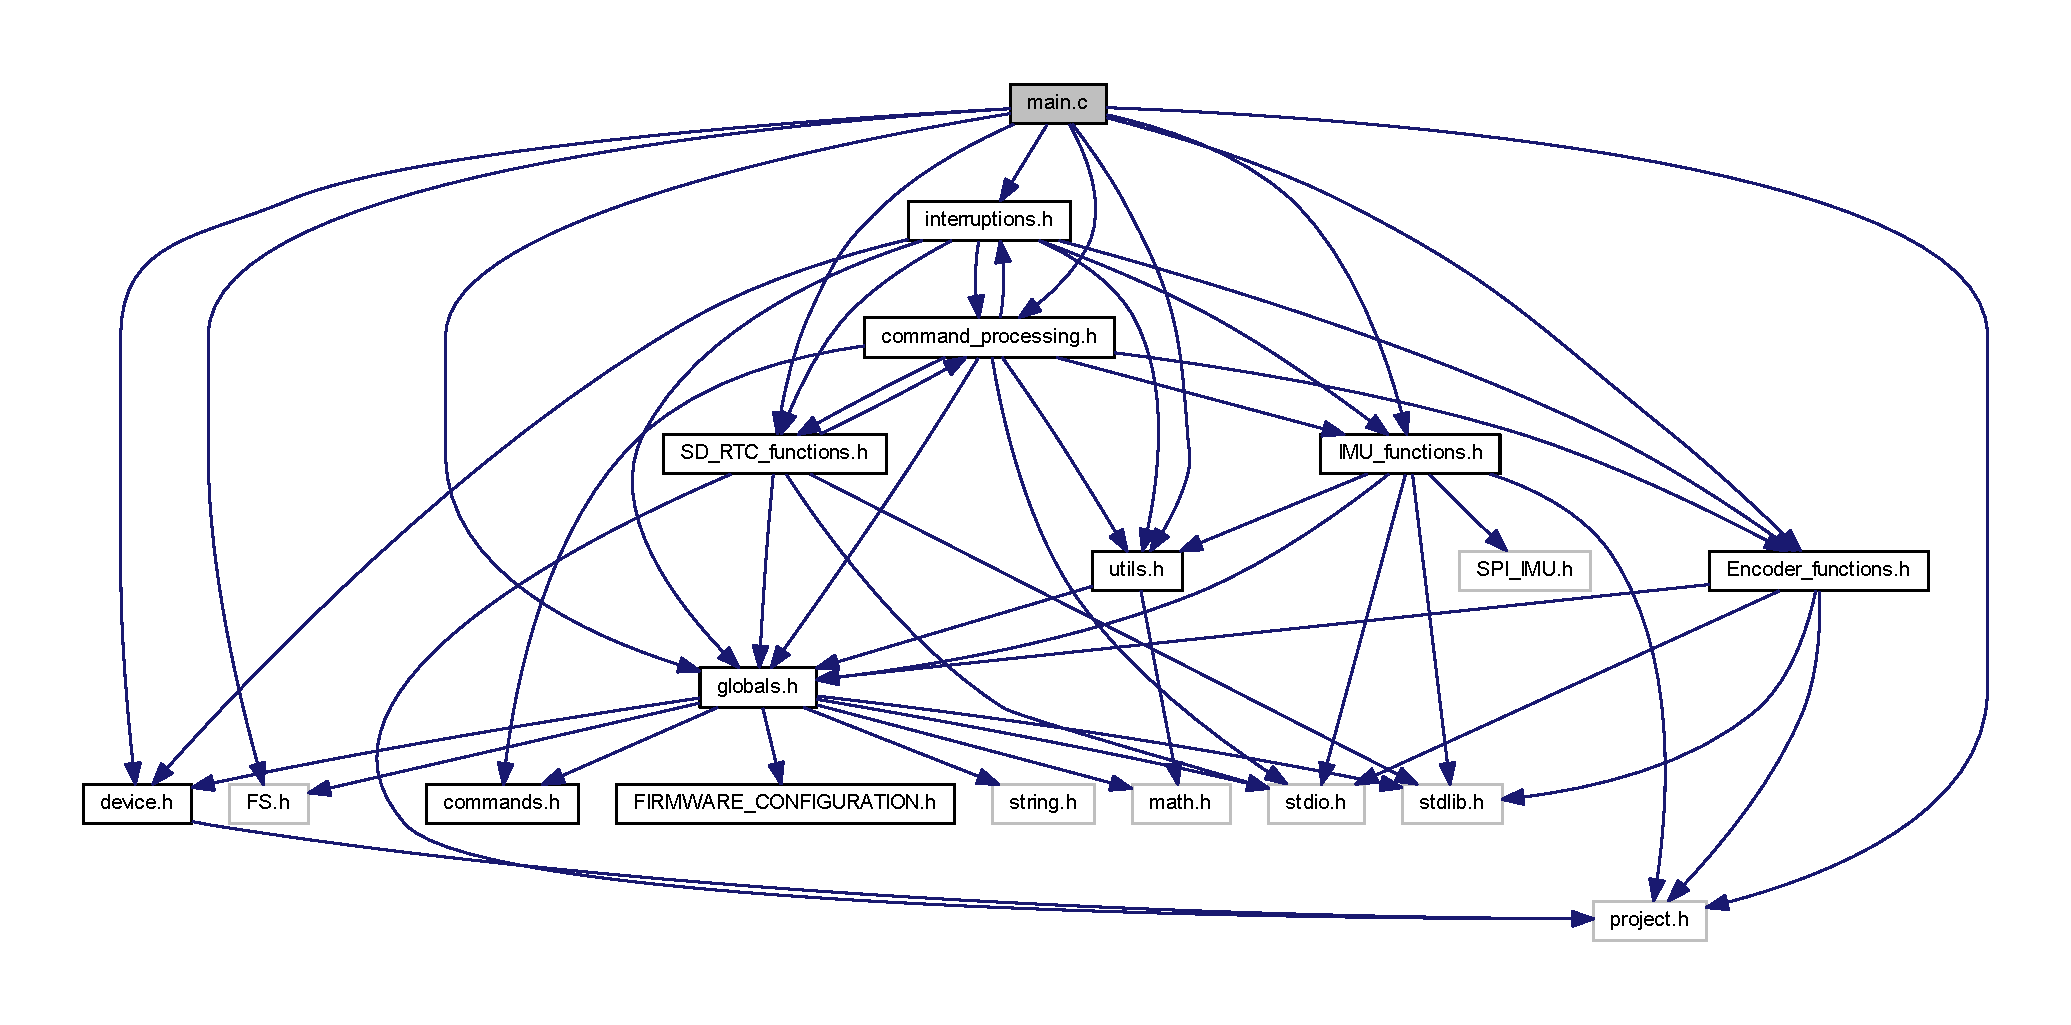
\includegraphics[width=350pt]{main_8c__incl}
\end{center}
\end{figure}
\subsection*{Functions}
\begin{DoxyCompactItemize}
\item 
\mbox{\label{main_8c_ae66f6b31b5ad750f1fe042a706a4e3d4}} 
int {\bfseries main} ()
\end{DoxyCompactItemize}


\subsection{Detailed Description}
Firmware main file. 

\begin{DoxyDate}{Date}
May 31, 2019 
\end{DoxyDate}
\begin{DoxyAuthor}{Author}
{\itshape Centro \char`\"{}\+E.\+Piaggio\char`\"{}} 
\end{DoxyAuthor}
\begin{DoxyCopyright}{Copyright}
(C) 2019 Centro \char`\"{}\+E.\+Piaggio\char`\"{}. All rights reserved. 
\end{DoxyCopyright}

\section{S\+D\+\_\+\+R\+T\+C\+\_\+functions.\+c File Reference}
\label{_s_d___r_t_c__functions_8c}\index{S\+D\+\_\+\+R\+T\+C\+\_\+functions.\+c@{S\+D\+\_\+\+R\+T\+C\+\_\+functions.\+c}}


Implementation of SD and R\+TC module functions.  


{\ttfamily \#include \char`\"{}S\+D\+\_\+\+R\+T\+C\+\_\+functions.\+h\char`\"{}}\newline
Include dependency graph for S\+D\+\_\+\+R\+T\+C\+\_\+functions.\+c\+:
% FIG 0
\subsection*{Functions}
\begin{DoxyCompactItemize}
\item 
\mbox{\label{_s_d___r_t_c__functions_8c_ae916e48139e2369b4295bc32b754cb09}} 
void {\bfseries D\+S1302\+\_\+write} (uint8 address, uint8 data\+\_\+wr)
\item 
\mbox{\label{_s_d___r_t_c__functions_8c_abf7dafb7cb2decd885c06cfd0d508a86}} 
void {\bfseries D\+S1302\+\_\+write\+Byte} (uint8 data\+\_\+wr)
\item 
\mbox{\label{_s_d___r_t_c__functions_8c_a648ecf3d4f3a92e6390945b156d5c98a}} 
uint8 {\bfseries D\+S1302\+\_\+read} (uint8 address)
\item 
\mbox{\label{_s_d___r_t_c__functions_8c_a961280caa20d802239a974419c19437e}} 
uint8 {\bfseries D\+S1302\+\_\+read\+Byte} ()
\item 
\mbox{\label{_s_d___r_t_c__functions_8c_a1f5533e91998b92926173f479322c7d9}} 
void {\bfseries shift\+Out\+\_\+\+R\+TC} (uint8 val)
\item 
\mbox{\label{_s_d___r_t_c__functions_8c_a262170705e582875a383a9f5c9b137a7}} 
void {\bfseries store\+\_\+\+R\+T\+C\+\_\+current\+\_\+time} ()
\item 
\mbox{\label{_s_d___r_t_c__functions_8c_ad0181162f59bf423c6d1dc1556afb6fc}} 
void {\bfseries set\+\_\+\+R\+T\+C\+\_\+time} ()
\item 
\mbox{\label{_s_d___r_t_c__functions_8c_a56466454f41dc875787a75f0d78b5602}} 
void {\bfseries Init\+S\+D\+\_\+\+FS} ()
\item 
\mbox{\label{_s_d___r_t_c__functions_8c_a5072914b0c92c6825bb196ba84b332c4}} 
void {\bfseries Write\+\_\+\+S\+D\+\_\+\+Param\+\_\+file} ()
\item 
\mbox{\label{_s_d___r_t_c__functions_8c_a9d056c3da2f8cd5c55be410e1959a485}} 
void {\bfseries Read\+\_\+\+S\+D\+\_\+\+Param} (char $\ast$info\+\_\+param, int n\+\_\+p)
\item 
\mbox{\label{_s_d___r_t_c__functions_8c_a0fbed516c0eda1c199a7641ca5c88692}} 
void {\bfseries Read\+\_\+\+S\+D\+\_\+\+Data} (char $\ast$info\+\_\+data, int n\+\_\+d)
\end{DoxyCompactItemize}


\subsection{Detailed Description}
Implementation of SD and R\+TC module functions. 

\begin{DoxyDate}{Date}
February 13, 2019 
\end{DoxyDate}
\begin{DoxyAuthor}{Author}
{\itshape Centro \char`\"{}\+E.\+Piaggio\char`\"{}} 
\end{DoxyAuthor}
\begin{DoxyCopyright}{Copyright}
(C) 2012-\/2016 qbrobotics. All rights reserved. 

(C) 2017-\/2019 Centro \char`\"{}\+E.\+Piaggio\char`\"{}. All rights reserved. 
\end{DoxyCopyright}

\section{S\+D\+\_\+\+R\+T\+C\+\_\+functions.\+h File Reference}
\label{_s_d___r_t_c__functions_8h}\index{S\+D\+\_\+\+R\+T\+C\+\_\+functions.\+h@{S\+D\+\_\+\+R\+T\+C\+\_\+functions.\+h}}


Definition of SD and R\+TC module functions.  


{\ttfamily \#include $<$project.\+h$>$}\newline
{\ttfamily \#include \char`\"{}globals.\+h\char`\"{}}\newline
{\ttfamily \#include $<$stdlib.\+h$>$}\newline
{\ttfamily \#include $<$stdio.\+h$>$}\newline
{\ttfamily \#include \char`\"{}command\+\_\+processing.\+h\char`\"{}}\newline
Include dependency graph for S\+D\+\_\+\+R\+T\+C\+\_\+functions.\+h\+:
% FIG 0
This graph shows which files directly or indirectly include this file\+:
% FIG 1
\subsection*{Macros}
\begin{DoxyCompactItemize}
\item 
\mbox{\label{_s_d___r_t_c__functions_8h_ac0bf5d4ed56463032c8735fdfd200da0}} 
\#define {\bfseries D\+S1302\+\_\+\+S\+E\+C\+O\+N\+D\+S\+\_\+\+WR}~0x80
\item 
\mbox{\label{_s_d___r_t_c__functions_8h_a83a504aca68d28a23ceb03b38384a509}} 
\#define {\bfseries D\+S1302\+\_\+\+S\+E\+C\+O\+N\+D\+S\+\_\+\+RD}~0x81
\item 
\mbox{\label{_s_d___r_t_c__functions_8h_a6afbe79491082889b12adc4d0f5edf2f}} 
\#define {\bfseries D\+S1302\+\_\+\+M\+I\+N\+U\+T\+E\+S\+\_\+\+WR}~0x82
\item 
\mbox{\label{_s_d___r_t_c__functions_8h_aef49f9b406cc8cbf23066e20382a17b9}} 
\#define {\bfseries D\+S1302\+\_\+\+M\+I\+N\+U\+T\+E\+S\+\_\+\+RD}~0x83
\item 
\mbox{\label{_s_d___r_t_c__functions_8h_a66cba43eaecb1e047f73265c11fe2aac}} 
\#define {\bfseries D\+S1302\+\_\+\+H\+O\+U\+R\+\_\+\+WR}~0x84
\item 
\mbox{\label{_s_d___r_t_c__functions_8h_a66a5375fea0bd8f39ccce55262571c87}} 
\#define {\bfseries D\+S1302\+\_\+\+H\+O\+U\+R\+\_\+\+RD}~0x85
\item 
\mbox{\label{_s_d___r_t_c__functions_8h_ab53e4481fe7704a79f469d7ae81d7ba8}} 
\#define {\bfseries D\+S1302\+\_\+\+D\+A\+T\+E\+\_\+\+WR}~0x86
\item 
\mbox{\label{_s_d___r_t_c__functions_8h_aa1076dbea29ed93a566866146adf87d3}} 
\#define {\bfseries D\+S1302\+\_\+\+D\+A\+T\+E\+\_\+\+RD}~0x87
\item 
\mbox{\label{_s_d___r_t_c__functions_8h_a5f4f20e5d9f7c19a35bee8823a2eecf8}} 
\#define {\bfseries D\+S1302\+\_\+\+M\+O\+N\+T\+H\+\_\+\+WR}~0x88
\item 
\mbox{\label{_s_d___r_t_c__functions_8h_acd933e6f2acf25bfae4c60b88c99292f}} 
\#define {\bfseries D\+S1302\+\_\+\+M\+O\+N\+T\+H\+\_\+\+RD}~0x89
\item 
\mbox{\label{_s_d___r_t_c__functions_8h_ab516547df86ac771c599ad840d806b69}} 
\#define {\bfseries D\+S1302\+\_\+\+Y\+E\+A\+R\+\_\+\+WR}~0x8C
\item 
\mbox{\label{_s_d___r_t_c__functions_8h_a37e2286ca2d3b25fa17400b5cdba8e43}} 
\#define {\bfseries D\+S1302\+\_\+\+Y\+E\+A\+R\+\_\+\+RD}~0x8D
\end{DoxyCompactItemize}
\subsection*{Functions}
\begin{DoxyCompactItemize}
\item 
\mbox{\label{_s_d___r_t_c__functions_8h_ae916e48139e2369b4295bc32b754cb09}} 
void {\bfseries D\+S1302\+\_\+write} (uint8 address, uint8 data\+\_\+wr)
\item 
\mbox{\label{_s_d___r_t_c__functions_8h_abf7dafb7cb2decd885c06cfd0d508a86}} 
void {\bfseries D\+S1302\+\_\+write\+Byte} (uint8 data\+\_\+wr)
\item 
\mbox{\label{_s_d___r_t_c__functions_8h_a648ecf3d4f3a92e6390945b156d5c98a}} 
uint8 {\bfseries D\+S1302\+\_\+read} (uint8 address)
\item 
\mbox{\label{_s_d___r_t_c__functions_8h_a961280caa20d802239a974419c19437e}} 
uint8 {\bfseries D\+S1302\+\_\+read\+Byte} ()
\item 
\mbox{\label{_s_d___r_t_c__functions_8h_a1f5533e91998b92926173f479322c7d9}} 
void {\bfseries shift\+Out\+\_\+\+R\+TC} (uint8 val)
\item 
\mbox{\label{_s_d___r_t_c__functions_8h_a262170705e582875a383a9f5c9b137a7}} 
void {\bfseries store\+\_\+\+R\+T\+C\+\_\+current\+\_\+time} ()
\item 
\mbox{\label{_s_d___r_t_c__functions_8h_ad0181162f59bf423c6d1dc1556afb6fc}} 
void {\bfseries set\+\_\+\+R\+T\+C\+\_\+time} ()
\item 
\mbox{\label{_s_d___r_t_c__functions_8h_a56466454f41dc875787a75f0d78b5602}} 
void {\bfseries Init\+S\+D\+\_\+\+FS} ()
\item 
\mbox{\label{_s_d___r_t_c__functions_8h_a5072914b0c92c6825bb196ba84b332c4}} 
void {\bfseries Write\+\_\+\+S\+D\+\_\+\+Param\+\_\+file} ()
\item 
\mbox{\label{_s_d___r_t_c__functions_8h_aba7e3006e26119efb8f8764b27fd31fa}} 
void {\bfseries Read\+\_\+\+S\+D\+\_\+\+Closed\+\_\+\+File} (char $\ast$, char $\ast$, int)
\item 
\mbox{\label{_s_d___r_t_c__functions_8h_abe0b3f7e7bb802a235c504c143bdad3f}} 
void {\bfseries Read\+\_\+\+S\+D\+\_\+\+Current\+\_\+\+Data} (char $\ast$, int)
\item 
\mbox{\label{_s_d___r_t_c__functions_8h_ac3a7b606d29e076ac0b4fa78b46a56a1}} 
int {\bfseries Get\+\_\+\+Directories\+List} (char $\ast$path, char directories\+\_\+list[3000][8], int first\+\_\+idx)
\item 
\mbox{\label{_s_d___r_t_c__functions_8h_abdf9196d903441c0febde4aa4d82f91f}} 
void {\bfseries Get\+\_\+\+S\+D\+\_\+\+FS} (char $\ast$)
\end{DoxyCompactItemize}


\subsection{Detailed Description}
Definition of SD and R\+TC module functions. 

\begin{DoxyDate}{Date}
March 20th, 2020 
\end{DoxyDate}
\begin{DoxyAuthor}{Author}
{\itshape Centro \char`\"{}\+E.\+Piaggio\char`\"{}} 
\end{DoxyAuthor}
\begin{DoxyCopyright}{Copyright}
(C) 2012-\/2016 qbrobotics. All rights reserved. 

(C) 2017-\/2020 Centro \char`\"{}\+E.\+Piaggio\char`\"{}. All rights reserved. 
\end{DoxyCopyright}

\doxysection{utils.\+c File Reference}
\label{utils_8c}\index{utils.c@{utils.c}}


Definition of utility functions.  


{\ttfamily \#include \char`\"{}utils.\+h\char`\"{}}\newline
Include dependency graph for utils.\+c\+:
% FIG 0
\doxysubsection*{Macros}
\begin{DoxyCompactItemize}
\item 
\mbox{\label{utils_8c_a52037c938e3c1b126c6277da5ca689d0}} 
\#define {\bfseries M}~65536
\begin{DoxyCompactList}\small\item\em Number of encoder ticks per turn. \end{DoxyCompactList}\end{DoxyCompactItemize}
\doxysubsection*{Functions}
\begin{DoxyCompactItemize}
\item 
int32 \textbf{ curr\+\_\+estim} (uint8 idx, int32 pos, int32 vel, int32 ref)
\item 
int32 \textbf{ filter} (int32 new\+\_\+value, struct \textbf{ st\+\_\+filter} $\ast$f)
\item 
uint32 \textbf{ my\+\_\+mod} (int32 val, int32 divisor)
\item 
void \textbf{ calibration} (void)
\item 
int \textbf{ calc\+\_\+turns\+\_\+fcn\+\_\+\+SH} (const int32 pos1, const int32 pos2, const int N1, const int N2, const int I1)
\item 
int \textbf{ calc\+\_\+turns\+\_\+fcn} (const int32 pos1, const int32 pos2, const int N1, const int N2, const int I1)
\item 
void \textbf{ check\+\_\+rest\+\_\+position} (void)
\item 
void \textbf{ LED\+\_\+control} (uint8 mode)
\item 
\mbox{\label{utils_8c_ae7eac41344d5679b9f7624357a88119d}} 
void {\bfseries battery\+\_\+management} ()
\item 
\mbox{\label{utils_8c_a1bea2981fd56850186356ea344e07e42}} 
void {\bfseries ADC\+\_\+\+Set\+\_\+\+N\+\_\+\+Channels} ()
\item 
\mbox{\label{utils_8c_a60ad0d7249bf56336e0908eaeec604e8}} 
void {\bfseries enable\+\_\+motor} (uint8 idx, uint8 val)
\item 
void \textbf{ reset\+\_\+counters} ()
\item 
\mbox{\label{utils_8c_a5e5346796220b271615a52428f6ec6ca}} 
float {\bfseries inv\+Sqrt} (float x)
\item 
\mbox{\label{utils_8c_a88d150c696b69e576a1dfb193266ae6a}} 
void {\bfseries v3\+\_\+normalize} (float v3\+\_\+in[3])
\item 
\mbox{\label{utils_8c_a2965058da02ba33e26af00cff2fcfec2}} 
void {\bfseries v4\+\_\+normalize} (float v4\+\_\+in[4])
\item 
void \textbf{ update\+\_\+\+EMG\+\_\+history} ()
\item 
\mbox{\label{utils_8c_a9b8b6ca7027bc3165c8786ae6d13f366}} 
void {\bfseries set\+\_\+motor\+\_\+driver\+\_\+type} ()
\end{DoxyCompactItemize}


\doxysubsection{Detailed Description}
Definition of utility functions. 

\begin{DoxyDate}{Date}
March 20th, 2020 
\end{DoxyDate}
\begin{DoxyAuthor}{Author}
{\itshape Centro \char`\"{}\+E.\+Piaggio\char`\"{}} 
\end{DoxyAuthor}
\begin{DoxyCopyright}{Copyright}
(C) 2012-\/2016 qbrobotics. All rights reserved. 

(C) 2017-\/2020 Centro \char`\"{}\+E.\+Piaggio\char`\"{}. All rights reserved. 
\end{DoxyCopyright}


\doxysubsection{Function Documentation}
\mbox{\label{utils_8c_ae7dc9eeaef91416fa3a148612ed75bf7}} 
\index{utils.c@{utils.c}!calc\_turns\_fcn@{calc\_turns\_fcn}}
\index{calc\_turns\_fcn@{calc\_turns\_fcn}!utils.c@{utils.c}}
\doxysubsubsection{calc\_turns\_fcn()}
{\footnotesize\ttfamily int calc\+\_\+turns\+\_\+fcn (\begin{DoxyParamCaption}\item[{const int32}]{pos1,  }\item[{const int32}]{pos2,  }\item[{const int}]{N1,  }\item[{const int}]{N2,  }\item[{const int}]{I1 }\end{DoxyParamCaption})}

This function is used at startup to reconstruct the correct turn of the shaft connected to the motor. Generic. It need two encoders to work.


\begin{DoxyParams}{Parameters}
{\em pos1} & First encoder position \\
\hline
{\em pos2} & Second encoder position\\
\hline
\end{DoxyParams}
\begin{DoxyReturn}{Returns}
Returns the number of turns of motor pulley at startup 
\end{DoxyReturn}
\mbox{\label{utils_8c_a73109b827d86a6936e0ca361d82d6328}} 
\index{utils.c@{utils.c}!calc\_turns\_fcn\_SH@{calc\_turns\_fcn\_SH}}
\index{calc\_turns\_fcn\_SH@{calc\_turns\_fcn\_SH}!utils.c@{utils.c}}
\doxysubsubsection{calc\_turns\_fcn\_SH()}
{\footnotesize\ttfamily int calc\+\_\+turns\+\_\+fcn\+\_\+\+SH (\begin{DoxyParamCaption}\item[{const int32}]{pos1,  }\item[{const int32}]{pos2,  }\item[{const int}]{N1,  }\item[{const int}]{N2,  }\item[{const int}]{I1 }\end{DoxyParamCaption})}

This function is used at startup to reconstruct the correct turn of the shaft connected to the motor. Only for Soft\+Hand 3.\+0. It need two encoders to work.


\begin{DoxyParams}{Parameters}
{\em pos1} & First encoder position \\
\hline
{\em pos2} & Second encoder position\\
\hline
\end{DoxyParams}
\begin{DoxyReturn}{Returns}
Returns the number of turns of motor pulley at startup 
\end{DoxyReturn}
\mbox{\label{utils_8c_a0b6a0b24c6bd8af032a6778166201f7e}} 
\index{utils.c@{utils.c}!calibration@{calibration}}
\index{calibration@{calibration}!utils.c@{utils.c}}
\doxysubsubsection{calibration()}
{\footnotesize\ttfamily void calibration (\begin{DoxyParamCaption}{ }\end{DoxyParamCaption})}

This function counts a series of hand opening and closing used to execute a calibration of the device. \mbox{\label{utils_8c_a13fca172b37b6f76749a864c1439b497}} 
\index{utils.c@{utils.c}!check\_rest\_position@{check\_rest\_position}}
\index{check\_rest\_position@{check\_rest\_position}!utils.c@{utils.c}}
\doxysubsubsection{check\_rest\_position()}
{\footnotesize\ttfamily void check\+\_\+rest\+\_\+position (\begin{DoxyParamCaption}{ }\end{DoxyParamCaption})}

This function checks for rest position and, in case, gives a position reference to Soft\+Hand. \mbox{\label{utils_8c_ad08aa627fe00611149acd407c0dbf4f6}} 
\index{utils.c@{utils.c}!curr\_estim@{curr\_estim}}
\index{curr\_estim@{curr\_estim}!utils.c@{utils.c}}
\doxysubsubsection{curr\_estim()}
{\footnotesize\ttfamily int32 curr\+\_\+estim (\begin{DoxyParamCaption}\item[{uint8}]{idx,  }\item[{int32}]{pos,  }\item[{int32}]{vel,  }\item[{int32}]{acc }\end{DoxyParamCaption})}

Function used to obtain current estimation through current lookup table.


\begin{DoxyParams}{Parameters}
{\em idx} & Index of motor. \\
\hline
{\em pos} & Position of the encoder in ticks. \\
\hline
{\em vel} & Speed of the encoder. \\
\hline
{\em accel} & Acceleration of the encoder\\
\hline
\end{DoxyParams}
\begin{DoxyReturn}{Returns}
Returns an estimation of the motor current, depending on its position, velocity and acceleration. 
\end{DoxyReturn}
\mbox{\label{utils_8c_a4ea945f48ed953ce9b0a6e51299d5677}} 
\index{utils.c@{utils.c}!filter@{filter}}
\index{filter@{filter}!utils.c@{utils.c}}
\doxysubsubsection{filter()}
{\footnotesize\ttfamily int32 filter (\begin{DoxyParamCaption}\item[{int32}]{value,  }\item[{struct \textbf{ st\+\_\+filter} $\ast$}]{f }\end{DoxyParamCaption})}

Generic low pass filter. The weighted average between the old value and the new one is executed.


\begin{DoxyParams}{Parameters}
{\em value} & New value of the filter. \\
\hline
{\em f} & Pointer to specific struct of type \doxyref{st\+\_\+filter}{p.}{structst__filter}. ~\newline
\\
\hline
\end{DoxyParams}
\begin{DoxyReturn}{Returns}
Returns the filtered current value 
\end{DoxyReturn}
\mbox{\label{utils_8c_a4443e9a681f8c13d317110b8017136c8}} 
\index{utils.c@{utils.c}!LED\_control@{LED\_control}}
\index{LED\_control@{LED\_control}!utils.c@{utils.c}}
\doxysubsubsection{LED\_control()}
{\footnotesize\ttfamily void LED\+\_\+control (\begin{DoxyParamCaption}\item[{uint8}]{mode }\end{DoxyParamCaption})}

This function switches between different LEDs condition depending on battery level of charge or needed maintenance. \mbox{\label{utils_8c_a01d3bb6c1fd469a6c530fb296e4fe0fe}} 
\index{utils.c@{utils.c}!my\_mod@{my\_mod}}
\index{my\_mod@{my\_mod}!utils.c@{utils.c}}
\doxysubsubsection{my\_mod()}
{\footnotesize\ttfamily uint32 my\+\_\+mod (\begin{DoxyParamCaption}\item[{int32}]{val,  }\item[{int32}]{divisor }\end{DoxyParamCaption})}

This function computes the module function, returning positive values regardless of wheter the value passed is negative


\begin{DoxyParams}{Parameters}
{\em val} & The value of which the module needs to be calculated \\
\hline
{\em divisor} & The divisor according to which the module is calculated \\
\hline
\end{DoxyParams}
\mbox{\label{utils_8c_a2640efff1e7b6f9c11615048ba43b0fd}} 
\index{utils.c@{utils.c}!reset\_counters@{reset\_counters}}
\index{reset\_counters@{reset\_counters}!utils.c@{utils.c}}
\doxysubsubsection{reset\_counters()}
{\footnotesize\ttfamily void reset\+\_\+counters (\begin{DoxyParamCaption}{ }\end{DoxyParamCaption})}

This function reset statistics counters \mbox{\label{utils_8c_aadf16dc795c83780e5b9eb5c2c5680b0}} 
\index{utils.c@{utils.c}!update\_EMG\_history@{update\_EMG\_history}}
\index{update\_EMG\_history@{update\_EMG\_history}!utils.c@{utils.c}}
\doxysubsubsection{update\_EMG\_history()}
{\footnotesize\ttfamily void update\+\_\+\+EMG\+\_\+history (\begin{DoxyParamCaption}{ }\end{DoxyParamCaption})}

This function updates the EMG history values with last availables. 
\section{utils.\+h File Reference}
\label{utils_8h}\index{utils.\+h@{utils.\+h}}


Utility functions declaration.  


{\ttfamily \#include \char`\"{}globals.\+h\char`\"{}}\newline
{\ttfamily \#include $<$math.\+h$>$}\newline
Include dependency graph for utils.\+h\+:
% FIG 0
This graph shows which files directly or indirectly include this file\+:
% FIG 1
\subsection*{Macros}
\begin{DoxyCompactItemize}
\item 
\#define \textbf{ Z\+M\+AX}~5
\item 
\#define \textbf{ Z\+E\+R\+O\+\_\+\+T\+OL}~100
\item 
\#define \textbf{ R\+E\+F\+S\+P\+E\+ED}~20
\item 
\#define \textbf{ S\+I\+GN}(A)~(((A) $>$=0) ? (1) \+: (-\/1))
\end{DoxyCompactItemize}
\subsection*{Functions}
\begin{Indent}\textbf{ Filters}\par
\begin{DoxyCompactItemize}
\item 
int32 \textbf{ filter} (int32 value, struct \textbf{ st\+\_\+filter} $\ast$f)
\end{DoxyCompactItemize}
\end{Indent}
\begin{Indent}\textbf{ Estimating current and difference}\par
\begin{DoxyCompactItemize}
\item 
int32 \textbf{ curr\+\_\+estim} (uint8 idx, int32 pos, int32 vel, int32 acc)
\end{DoxyCompactItemize}
\end{Indent}
\begin{Indent}\textbf{ Utility functions}\par
\begin{DoxyCompactItemize}
\item 
uint32 \textbf{ my\+\_\+mod} (int32 val, int32 divisor)
\item 
int \textbf{ calc\+\_\+turns\+\_\+fcn\+\_\+\+SH} (const int32 pos1, const int32 pos2, const int N1, const int N2, const int I1)
\item 
int \textbf{ calc\+\_\+turns\+\_\+fcn} (const int32 pos1, const int32 pos2, const int N1, const int N2, const int I1)
\item 
void \textbf{ calibration} ()
\item 
void \textbf{ check\+\_\+rest\+\_\+position} ()
\item 
void \textbf{ L\+E\+D\+\_\+control} (uint8 mode)
\item 
\mbox{\label{utils_8h_ae7eac41344d5679b9f7624357a88119d}} 
void {\bfseries battery\+\_\+management} ()
\item 
\mbox{\label{utils_8h_a1bea2981fd56850186356ea344e07e42}} 
void {\bfseries A\+D\+C\+\_\+\+Set\+\_\+\+N\+\_\+\+Channels} ()
\item 
\mbox{\label{utils_8h_a60ad0d7249bf56336e0908eaeec604e8}} 
void {\bfseries enable\+\_\+motor} (uint8 idx, uint8 val)
\item 
void \textbf{ reset\+\_\+counters} ()
\item 
\mbox{\label{utils_8h_a5e5346796220b271615a52428f6ec6ca}} 
float {\bfseries inv\+Sqrt} (float x)
\item 
\mbox{\label{utils_8h_a88d150c696b69e576a1dfb193266ae6a}} 
void {\bfseries v3\+\_\+normalize} (float v3\+\_\+in[3])
\item 
\mbox{\label{utils_8h_a2965058da02ba33e26af00cff2fcfec2}} 
void {\bfseries v4\+\_\+normalize} (float v4\+\_\+in[4])
\end{DoxyCompactItemize}
\end{Indent}


\subsection{Detailed Description}
Utility functions declaration. 

\begin{DoxyDate}{Date}
March 20th, 2020 
\end{DoxyDate}
\begin{DoxyAuthor}{Author}
{\itshape Centro \char`\"{}\+E.\+Piaggio\char`\"{}} 
\end{DoxyAuthor}
\begin{DoxyCopyright}{Copyright}
(C) 2012-\/2016 qbrobotics. All rights reserved. 

(C) 2017-\/2020 Centro \char`\"{}\+E.\+Piaggio\char`\"{}. All rights reserved. 
\end{DoxyCopyright}


\subsection{Macro Definition Documentation}
\mbox{\label{utils_8h_a398d0c26e6af88fbdc96f871b7c3495e}} 
\index{utils.\+h@{utils.\+h}!R\+E\+F\+S\+P\+E\+ED@{R\+E\+F\+S\+P\+E\+ED}}
\index{R\+E\+F\+S\+P\+E\+ED@{R\+E\+F\+S\+P\+E\+ED}!utils.\+h@{utils.\+h}}
\subsubsection{R\+E\+F\+S\+P\+E\+ED}
{\footnotesize\ttfamily \#define R\+E\+F\+S\+P\+E\+ED~20}

Constant depending on P\+ID values. \mbox{\label{utils_8h_a8c7db0cde6d591a5abad279ba92ef021}} 
\index{utils.\+h@{utils.\+h}!S\+I\+GN@{S\+I\+GN}}
\index{S\+I\+GN@{S\+I\+GN}!utils.\+h@{utils.\+h}}
\subsubsection{S\+I\+GN}
{\footnotesize\ttfamily \#define S\+I\+GN(\begin{DoxyParamCaption}\item[{}]{A }\end{DoxyParamCaption})~(((A) $>$=0) ? (1) \+: (-\/1))}

Sign calculation function. \mbox{\label{utils_8h_a2d55df83bcb11e53743ff6732e4bf7c1}} 
\index{utils.\+h@{utils.\+h}!Z\+E\+R\+O\+\_\+\+T\+OL@{Z\+E\+R\+O\+\_\+\+T\+OL}}
\index{Z\+E\+R\+O\+\_\+\+T\+OL@{Z\+E\+R\+O\+\_\+\+T\+OL}!utils.\+h@{utils.\+h}}
\subsubsection{Z\+E\+R\+O\+\_\+\+T\+OL}
{\footnotesize\ttfamily \#define Z\+E\+R\+O\+\_\+\+T\+OL~100}

Deadband used to put to zero the virtual position due to the fact that the friction model has errors when the position is near to zero. \mbox{\label{utils_8h_a131010b0d7e64a592f782aec28c6a4d8}} 
\index{utils.\+h@{utils.\+h}!Z\+M\+AX@{Z\+M\+AX}}
\index{Z\+M\+AX@{Z\+M\+AX}!utils.\+h@{utils.\+h}}
\subsubsection{Z\+M\+AX}
{\footnotesize\ttfamily \#define Z\+M\+AX~5}

Constant useful for current estimation procedure. 

\subsection{Function Documentation}
\mbox{\label{utils_8h_ae7dc9eeaef91416fa3a148612ed75bf7}} 
\index{utils.\+h@{utils.\+h}!calc\+\_\+turns\+\_\+fcn@{calc\+\_\+turns\+\_\+fcn}}
\index{calc\+\_\+turns\+\_\+fcn@{calc\+\_\+turns\+\_\+fcn}!utils.\+h@{utils.\+h}}
\subsubsection{calc\+\_\+turns\+\_\+fcn()}
{\footnotesize\ttfamily int calc\+\_\+turns\+\_\+fcn (\begin{DoxyParamCaption}\item[{const int32}]{pos1,  }\item[{const int32}]{pos2,  }\item[{const int}]{N1,  }\item[{const int}]{N2,  }\item[{const int}]{I1 }\end{DoxyParamCaption})}

This function is used at startup to reconstruct the correct turn of the shaft connected to the motor. Generic. It need two encoders to work.


\begin{DoxyParams}{Parameters}
{\em pos1} & First encoder position \\
\hline
{\em pos2} & Second encoder position\\
\hline
\end{DoxyParams}
\begin{DoxyReturn}{Returns}
Returns the number of turns of motor pulley at startup 
\end{DoxyReturn}
\mbox{\label{utils_8h_a73109b827d86a6936e0ca361d82d6328}} 
\index{utils.\+h@{utils.\+h}!calc\+\_\+turns\+\_\+fcn\+\_\+\+SH@{calc\+\_\+turns\+\_\+fcn\+\_\+\+SH}}
\index{calc\+\_\+turns\+\_\+fcn\+\_\+\+SH@{calc\+\_\+turns\+\_\+fcn\+\_\+\+SH}!utils.\+h@{utils.\+h}}
\subsubsection{calc\+\_\+turns\+\_\+fcn\+\_\+\+S\+H()}
{\footnotesize\ttfamily int calc\+\_\+turns\+\_\+fcn\+\_\+\+SH (\begin{DoxyParamCaption}\item[{const int32}]{pos1,  }\item[{const int32}]{pos2,  }\item[{const int}]{N1,  }\item[{const int}]{N2,  }\item[{const int}]{I1 }\end{DoxyParamCaption})}

This function is used at startup to reconstruct the correct turn of the shaft connected to the motor. Only for Soft\+Hand 3.\+0. It need two encoders to work.


\begin{DoxyParams}{Parameters}
{\em pos1} & First encoder position \\
\hline
{\em pos2} & Second encoder position\\
\hline
\end{DoxyParams}
\begin{DoxyReturn}{Returns}
Returns the number of turns of motor pulley at startup 
\end{DoxyReturn}
\mbox{\label{utils_8h_a6d9dc88d64cd1f74a30fd0e404a3bb31}} 
\index{utils.\+h@{utils.\+h}!calibration@{calibration}}
\index{calibration@{calibration}!utils.\+h@{utils.\+h}}
\subsubsection{calibration()}
{\footnotesize\ttfamily void calibration (\begin{DoxyParamCaption}{ }\end{DoxyParamCaption})}

This function counts a series of hand opening and closing used to execute a calibration of the device. \mbox{\label{utils_8h_a2cb024aea0170c085d18670f5a851df8}} 
\index{utils.\+h@{utils.\+h}!check\+\_\+rest\+\_\+position@{check\+\_\+rest\+\_\+position}}
\index{check\+\_\+rest\+\_\+position@{check\+\_\+rest\+\_\+position}!utils.\+h@{utils.\+h}}
\subsubsection{check\+\_\+rest\+\_\+position()}
{\footnotesize\ttfamily void check\+\_\+rest\+\_\+position (\begin{DoxyParamCaption}{ }\end{DoxyParamCaption})}

This function checks for rest position and, in case, gives a position reference to Soft\+Hand. \mbox{\label{utils_8h_a284a90898751a15b0303f688f19948b9}} 
\index{utils.\+h@{utils.\+h}!curr\+\_\+estim@{curr\+\_\+estim}}
\index{curr\+\_\+estim@{curr\+\_\+estim}!utils.\+h@{utils.\+h}}
\subsubsection{curr\+\_\+estim()}
{\footnotesize\ttfamily int32 curr\+\_\+estim (\begin{DoxyParamCaption}\item[{uint8}]{idx,  }\item[{int32}]{pos,  }\item[{int32}]{vel,  }\item[{int32}]{acc }\end{DoxyParamCaption})}

Function used to obtain current estimation through current lookup table.


\begin{DoxyParams}{Parameters}
{\em idx} & Index of motor. \\
\hline
{\em pos} & Position of the encoder in ticks. \\
\hline
{\em vel} & Speed of the encoder. \\
\hline
{\em accel} & Acceleration of the encoder\\
\hline
\end{DoxyParams}
\begin{DoxyReturn}{Returns}
Returns an estimation of the motor current, depending on its position, velocity and acceleration. 
\end{DoxyReturn}
\mbox{\label{utils_8h_aa404d0e01f2ab2318d323c7ef8fa6c5a}} 
\index{utils.\+h@{utils.\+h}!filter@{filter}}
\index{filter@{filter}!utils.\+h@{utils.\+h}}
\subsubsection{filter()}
{\footnotesize\ttfamily int32 filter (\begin{DoxyParamCaption}\item[{int32}]{value,  }\item[{struct \textbf{ st\+\_\+filter} $\ast$}]{f }\end{DoxyParamCaption})}

Generic low pass filter. The weighted average between the old value and the new one is executed.


\begin{DoxyParams}{Parameters}
{\em value} & New value of the filter. \\
\hline
{\em f} & Pointer to specific struct of type \doxyref{st\+\_\+filter}{p.}{structst__filter}.\\
\hline
\end{DoxyParams}
\begin{DoxyReturn}{Returns}
Returns the filtered current value 
\end{DoxyReturn}
\mbox{\label{utils_8h_a4443e9a681f8c13d317110b8017136c8}} 
\index{utils.\+h@{utils.\+h}!L\+E\+D\+\_\+control@{L\+E\+D\+\_\+control}}
\index{L\+E\+D\+\_\+control@{L\+E\+D\+\_\+control}!utils.\+h@{utils.\+h}}
\subsubsection{L\+E\+D\+\_\+control()}
{\footnotesize\ttfamily void L\+E\+D\+\_\+control (\begin{DoxyParamCaption}\item[{uint8}]{mode }\end{DoxyParamCaption})}

This function switches between different L\+E\+Ds condition depending on battery level of charge or needed maintenance. \mbox{\label{utils_8h_a01d3bb6c1fd469a6c530fb296e4fe0fe}} 
\index{utils.\+h@{utils.\+h}!my\+\_\+mod@{my\+\_\+mod}}
\index{my\+\_\+mod@{my\+\_\+mod}!utils.\+h@{utils.\+h}}
\subsubsection{my\+\_\+mod()}
{\footnotesize\ttfamily uint32 my\+\_\+mod (\begin{DoxyParamCaption}\item[{int32}]{val,  }\item[{int32}]{divisor }\end{DoxyParamCaption})}

This function computes the module function, returning positive values regardless of wheter the value passed is negative


\begin{DoxyParams}{Parameters}
{\em val} & The value of which the module needs to be calculated \\
\hline
{\em divisor} & The divisor according to which the module is calculated \\
\hline
\end{DoxyParams}
\mbox{\label{utils_8h_a2640efff1e7b6f9c11615048ba43b0fd}} 
\index{utils.\+h@{utils.\+h}!reset\+\_\+counters@{reset\+\_\+counters}}
\index{reset\+\_\+counters@{reset\+\_\+counters}!utils.\+h@{utils.\+h}}
\subsubsection{reset\+\_\+counters()}
{\footnotesize\ttfamily void reset\+\_\+counters (\begin{DoxyParamCaption}{ }\end{DoxyParamCaption})}

This function reset statistics counters 
%--- End generated contents ---

% Index
\backmatter
\newpage
\phantomsection
\clearemptydoublepage
\addcontentsline{toc}{chapter}{Index}
\printindex

\end{document}
